\documentclass[a4paper]{article}
\usepackage{pgf,tikz,pgfplots}
\usetikzlibrary{arrows,decorations.markings}
\pgfplotsset{compat=1.15}
\usepackage{mathrsfs}
\usetikzlibrary{arrows}
%% Language and font encodings
\usepackage[english]{babel}
\usepackage[utf8x]{inputenc}
\usepackage[T1]{fontenc}
\usepackage{float}
%% Sets page size and margins
\usepackage[a4paper,top=3cm,bottom=2cm,left=3cm,right=3cm,marginparwidth=1.75cm]{geometry}
\usepackage{fancyhdr}
\usepackage[framemethod=TikZ]{mdframed}
\pagestyle{fancy}
%% Useful packages
\usepackage{tensor}
\usepackage{amsmath}
\usepackage{amsthm}
\usepackage{enumitem}
\usepackage{eqnarray}
\usepackage{float}
\usepackage{esint}
\usepackage{wrapfig}
\usepackage{gensymb}
\usepackage{lipsum}
\usepackage{amssymb}
\usepackage{array}
\usepackage{tikz}
\usetikzlibrary{decorations.markings}
\tikzset{->-/.style={decoration={
  markings,
  mark=at position #1 with {\arrow{>}}},postaction={decorate}}}
\tikzset{-<-/.style={decoration={
  markings,
  mark=at position #1 with {\arrow{<}}},postaction={decorate}}}
\usepackage[colorlinks=true, allcolors=blue]{hyperref}
\usepackage{graphicx}
\usepackage{amsmath}
\usepackage{amssymb}
\usepackage{graphicx}
\usepackage[colorlinks=true, allcolors=blue]{hyperref}
\usepackage{mathtools}
\DeclareMathOperator{\Proj}{Proj}
\DeclareMathOperator{\res}{res}
\DeclareMathOperator{\lcm}{lcm}
\DeclareMathOperator{\cosec}{cosec}
\DeclareMathOperator{\sgn}{sgn}
\DeclareMathOperator{\Span}{span}
\DeclareMathOperator{\nullity}{nullity}
\DeclarePairedDelimiter\floor{\lfloor}{\rfloor}
\DeclareMathOperator{\Res}{Res}
\DeclareMathOperator{\rank}{rank}
\DeclareMathOperator{\Ker}{Ker}
\DeclareMathOperator{\R}{R}
\DeclareMathOperator{\Tr}{Tr}
\DeclareMathOperator{\diag}{diag}
\DeclareMathOperator{\Log}{Log}
\DeclareMathOperator{\sech}{sech}
\DeclareMathOperator{\Var}{Var}
\newtheorem{ans}{Answer}[section]
\newtheorem{remarks}{Remarks}[section]
\newtheorem{note}{Note}[section]
\newtheorem{eg}{Example}[section]
\newtheorem{notation}{Notation}[section]
\definecolor{darkblue}{RGB}{	0, 0, 139}
\newtheoremstyle{new}% <name>
{2pt}% <Space above>
{2pt}% <Space below>
{\color{darkblue}}% Body font
{}% <Indent amount>
{\bfseries\color{black}}% Theorem head font
{:}% <Punctuation after theorem head>
{.5em}% <Space after theorem headi>
{}% <Theorem head spec (can be left empty, meaning `normal')>
\theoremstyle{new}
\newtheorem{law}{Law}[section]
\newtheorem{defi}{Definition}[section]
\newtheorem{thm}{Theorem}[section]
\newtheorem{prop}{Proposition}[section]
\newtheorem{lemma}{Lemma}[section]
\newtheorem{cor}{Corollary}[section]
\newtheorem{qns}{Problem}[section]
\setlength{\parindent}{0cm}
\title{\textbf{Part II TP1 (Theoretical Physics 1)}}
\author{Tai Yingzhe, Tommy (ytt26)}
\date{}
\setlength{\parindent}{0cm}
\begin{document}
\maketitle
{\small\tableofcontents}
\subsection*{Acknowledgements:}
Many thanks to my demonstrators Joseph Smith, and the lecturer Ben Gripaios for their guidance. Some parts of this notes are heavily influenced by the Part III DAMTP courses Quantum Field Theory and Statistical Field Theory, as well as, the Part II DAMTP course Classical Mechanics.
\newpage
\section{Lagrangian and Hamiltonian Mechanics}
\subsection{Lagrangian Formalism}
\subsubsection{Generalized Coordinates}
While Newtonian mechanics uses vectors, the Lagrangian approach is more flexible. A system with $n$ degrees of freedom requires $n$ independent generalized coordinates $q_i(t)$, $i=1$, ..., $n$, to specify its configuration. The generalized velocities are $\dot{q}_i=\frac{dq_i}{dt}$. Why do we do this? This is useful
\begin{itemize}
    \item in non-Cartesian coordinates, for example, polar coordinates for problems with circular or spherical symmetry. 
    \item for systems with constraints, for example, confining surfaces, curves, strings, rods, etc.
\end{itemize}
\begin{defi}[Lagrangian Mechanics]
Lagrangian mechanics deals mostly with systems that are conservative (ideal, non-dissipative). Their dynamics can be derived from a scalar function, the Lagrangian $\mathcal{L}(\mathbf{q},\mathbf{\dot{q}},t)$ where $\mathbf{q}$ stands for $(q_1,...,q_n)$ and $\mathbf{\dot{q}}$ stands for $(\dot{q}_1,...,\dot{q}_n)$, $\frac{\partial\mathcal{L}}{\partial\mathbf{q}}$ stands for $(\frac{\partial\mathcal{L}}{\partial q_1},...,\frac{\partial\mathcal{L}}{\partial q_n})$, $\mathbf{q}\cdot\mathbf{p}=q_ip_i$, etc.
\end{defi}
\subsubsection{Hamilton's Principle}
\begin{defi}[Action]
If a system evolves from an initial configuration $\mathbf{q_1}=\mathbf{q}(t_1)$ to a final configuration $\mathbf{q_2}=\mathbf{q}(t_2)$, the action is defined as a functional of the path $\mathbf{q}(t)$ taken in configuration space.
$$S[\mathbf{q}]=\int_{t_1}^{t_2}\mathcal{L}(\mathbf{q},\mathbf{\dot{q}},t)dt$$
\end{defi}
\begin{defi}[Hamilton's principle]
The Hamilton's principle states that the physical path is such that the action has a stationary value, i.e. the first variation $\delta S=\delta\int\mathcal{L}dt=0$, subject to $\mathbf{q}(t_1)$ and $\mathbf{q}(t_2)$ being fixed. 
\end{defi}
\begin{prop}
Hamilton's principle require the Lagrangian to satisfy the Euler-Lagrange equation for the variable $q_i$.
$$\frac{\partial\mathcal{L}}{\partial q_i}-\frac{d}{dt}\frac{\partial\mathcal{L}}{\partial\dot{q}_i}=0$$
\end{prop}
\begin{proof}
According to the calculus of variations, Hamilton's Principle mean that the functional derivative vanishes, i.e. $\frac{\partial S}{\partial q_i}=0$ for each $i=1,...,n$. This is the Euler-Lagrange equation for the variable $q_i$. The variation $\delta$ commutes with integration and differentiation. Also, $\delta\int\mathcal{L}dt=\int\delta\mathcal{L}dt$, and $\delta(\dot{q}_i)=\frac{d}{dt}(\delta q_i)=\delta\dot{q}_i$. We have
$$\delta S=\int_{t_1}^{t_2}\delta\mathcal{L}dt=\int_{t_1}^{t_2}\sum_{i=1}^n\bigg(\frac{\partial\mathcal{L}}{\partial q_i}\delta q_i+\frac{\partial\mathcal{L}}{\partial\dot{q}_i}\delta\dot{q}_i\bigg)dt=\int_{t_1}^{t_2}\sum_{i=1}^n\bigg(\frac{\partial\mathcal{L}}{\partial q_i}-\frac{d}{dt}\frac{\partial\mathcal{L}}{\partial \dot{q}_i}\bigg)\delta q_idt+\bigg[\sum_{i=1}^n\frac{\partial\mathcal{L}}{\partial\dot{q}_i}\delta q_i\bigg]_{t_1}^{t_2}$$
If $\delta S$ is to vanish for all variations $\delta q_i$ and vanish at the endpoints, then we obtain the Euler-Lagrange equations.
\end{proof}
\begin{remarks}
In analytical mechanics, we call these the Lagrange's equations and interpret them as the equations of motion of the system:
$$\frac{d}{dt}\frac{\partial\mathcal{L}}{\partial\dot{q}_i}=\frac{\partial\mathcal{L}}{\partial q_i}\iff\frac{d}{dt}\frac{\partial\mathcal{L}}{\partial\mathbf{\dot{q}}}=\frac{\partial\mathcal{L}}{\partial\mathbf{q}}$$
Since $\mathcal{L}$ depends on $\mathbf{q}$ and $\mathbf{\dot{q}}$, these are $n$ second order ODEs for $q_i(t)$. In general, they are non-linear. We can identify the LHS of Lagrange equations as $\frac{dp_i}{dt}$ where $p_i=\frac{\partial\mathcal{L}}{\partial\dot{q}_i}$ is the generalized momentum, associated with the generalized coordinate $q_i$, i.e. conjugate to $q_i$.
\end{remarks}
\begin{prop}
Lagrangian is unique up to an additive/multiplicative constant and a total time derivative term (of a function independent of $\dot{q}$).
\end{prop}
\begin{proof}
The constant case is obvious. Add $\frac{d}{dt}f(\mathbf{q},t)$ to $\mathcal{L}$ and apply EL equation:
$$\mathcal{L}'=\mathcal{L}+\frac{\partial f}{\partial t}+\frac{\partial f}{\partial\mathbf{q}}\cdot\mathbf{\dot{q}}\implies\frac{d}{dt}\frac{\partial\mathcal{L}'}{\partial\mathbf{\dot{q}}}=\frac{d}{dt}\frac{\partial\mathcal{L}}{\partial\mathbf{\dot{q}}}+\frac{\partial}{\partial\mathbf{q}}\frac{df}{dt},\quad\frac{\partial\mathcal{L}'}{\partial\mathbf{q}}=\frac{\partial\mathcal{L}}{\partial\mathbf{q}}+\frac{\partial}{\partial\mathbf{q}}\frac{df}{dt}$$
Hence, $\mathcal{L}$ and $\mathcal{L}'$ both give the same equations of motion. In the proof for the Euler-Lagrange equations, we add $\frac{d}{dt}f(\mathbf{q},t)$ to the action $S=\int\mathcal{L}dt$, then we obtain the quantity $f(\mathbf{q},t_2)-f(\mathbf{q},t_1)$ which is independent of the path.
\end{proof}
\subsubsection{Constraints}
Often we deal with systems of particles whose motion is constrained. 
\begin{eg}
For example, in a rigid body, $|\mathbf{r_i}-\mathbf{r_j}|$ is a constant $\forall i,j$, i.e. any pair of particles. In another example, in a simple pendulum, the particle can only move on a 1D circle. Forces of constraint are required to enforce these conditions. In the Newtonian approach, we introduce these forces explicitly and eliminate them algebraically. The Lagrangian method handles them more easily.
\end{eg}
\begin{prop}
Consider a system of $N$ particles moving in $\mathcal{D}$-dimensions, subject to $M$ independent holonomic constraints of the form 
$$f_m(\mathbf{r_1},...,\mathbf{r_N},t)=0$$
for $m=1,...,M$. The constraints restrict the possible configurations to a surface in $\mathbb{R}^{\mathcal{D}N}$ of dimension $n=\mathcal{D}N-M$, called the configuration space (or manifold) of this constrained system. The resulting system has $n$ degrees of freedom.
\end{prop}
\begin{defi}[Scleronomic, rhenomic constraints]
Scleronomic constraints do not depend explicitly on time, while the rheonomic constraints do. 
\end{defi}
\begin{eg}
A particle in 3D confined to move along a moving wire, is subject to two rheonomic constraints and has one degree of freedom. 
\end{eg}
\begin{prop}
The Euler-Lagrange equations with constraints $f_m(\mathbf{r_1},\dots,\mathbf{r_N},t)=0$ are
$$\frac{d}{dt}\frac{\partial\mathcal{L}}{\partial\mathbf{\dot{r}_i}}-\frac{\partial\mathcal{L}}{\partial\mathbf{r_i}}-\sum_{m=1}^M\lambda_m(t)\frac{\partial f_m}{\partial\mathbf{r_i}}=0$$
for the $i$th particle. The last term is associated with forces of constraint, which can be eliminated algebraically as in the Newtonian method.
\end{prop}
\begin{proof}
To enforce $f_m=0$ at every instant $t\in(t_1,t_2)$, we require a time-dependent Lagrange multiplier $\lambda_m(t)$. The variation of action $\int\mathcal{L}dt$ is thus subject to the constraints $f_m=0$. This is equivalent to an unconstrained variation of $\int(\mathcal{L}-\sum_{m=1}^M\lambda_m(t)f_m)dt$, i.e.
$$0=\delta S=\int\delta\mathcal{L}-\sum_{i=1}^N\sum_{m=1}^M\lambda_m(t)\frac{\partial f}{\partial\mathbf{r}_i}\cdot\delta\mathbf{r}_idt=\int\bigg[\frac{\partial\mathcal{L}}{\partial \mathbf{r_i}}-\frac{d}{dt}\bigg(\frac{\partial\mathcal{L}}{\partial\mathbf{\dot{r}_i}}\bigg)-\sum_m\lambda_m\frac{\partial f_m}{\partial \mathbf{r_i}}\bigg]\cdot\delta\mathbf{r_i}dt$$
This gives the modified Lagrange equations for the $i$th particle. 
\end{proof}
\begin{prop}
A better approach is to solve the equations of constraint by introducing $n$ (dimension of configuration space) independent generalized coordinates $\{q_1,...,q_n\}$ that uniquely specify the configuration subject to all constraints. We can then write $\mathbf{r_i}(\mathbf{q})$ and $\mathbf{r_i}(\mathbf{q},t)$ for scleronomic and rheonomic constraints. For each $i=1,...,n$, we obtain the unmodified Lagrange equations
$$\frac{d}{dt}\frac{\partial\mathcal{L}}{\partial\dot{q}_i}=\frac{\partial\mathcal{L}}{\partial q_i}$$
because the $f_m$ do not depend on $q_1,...,q_n$.
\end{prop}
\begin{eg}
Consider a 2D simple pendulum of length $l$. The constraints $f=|\mathbf{r}|-l=0$ produces a force of constraint $-\lambda\boldsymbol{\nabla}f=-\lambda\frac{\mathbf{r}}{|\mathbf{r}|}$. Here, $\lambda$ is the tension in the string, or the normal reaction from a surface, required to constrain the particle to a circle. If instead of $(x,y)$, we use the generalized coordinate $\theta$, we can just solve $\frac{d}{dt}\frac{\partial\mathcal{L}}{\partial\dot{\theta}}=\frac{\partial\mathcal{L}}{\partial\theta}$ and ignore the constraint.
\end{eg}
\begin{eg}
Examples of non-holonomic constraints: inequalities, for example, particle bouncing on a table, i.e. $z\geq0$, non-integrable constraints involving velocities, for example, a sphere or a disc rolling on a surface. Surprisingly, for the case of a cylinder, the problem is integrable.
\end{eg}
\subsubsection{Symmetries and Conservation Laws}
\begin{defi}[Cyclic coordinate]
If $\mathcal{L}$ does not depend on a particular coordinate, then that coordinate is ignorable and is known as a cyclic coordinate.
\end{defi}
\begin{thm}[Conservation of momentum]
If the Lagrangian $\mathcal{L}$ does not depend on a generalized coordinate $q_k$, then the conjugate momenta $p_k:=\frac{\partial\mathcal{L}}{\partial\dot{q}_k}$ is constant in time.
\end{thm}
\begin{proof}
Lagrange's equations for $q_k$ then reduces to $\frac{d}{dt}\frac{\partial\mathcal{L}}{\partial\dot{q}_k}=0$ which implies the conservation law: $\frac{\partial\mathcal{L}}{\partial\dot{q}_k}:=p_k$, the conjugate momenta, is constant in time.
\end{proof}
\begin{remarks}
Conjugate momenta includes linear momentum and angular momentum (where the cyclic coordinate here is an angular coordinate).
\end{remarks}
\begin{prop}
The kinetic energy is a positive definite, homogeneous quadratic function of the generalized velocities.
$$T=\sum_{i=1}^N\sum_{j=1}^N\frac{1}{2}T_{ij}(\mathbf{q})\dot{q}_i\dot{q}_j$$ 
where $T_{ij}(\mathbf{q})=\sum_{k=1}^Nm_k\frac{\partial\mathbf{r_k}}{\partial q_i}\frac{\partial\mathbf{r_k}}{\partial q_j}$ is a positive definite symmetric matrix.
\end{prop}
\begin{proof}
To rewrite the kinetic energy in terms of the generalized coordinates and velocities, consider $\mathbf{\dot{r}_k}=\frac{\partial\mathbf{r_k}}{\partial t}+\sum_{i=1}^n\frac{\partial\mathbf{r_k}}{\partial\mathbf{q_i}}\mathbf{\dot{q}_i}$. If the constraints are scleronomic, $\frac{\partial\mathbf{r_k}}{\partial t}=0$. Then the kinetic energy is
$$T=\sum_{k=1}^N\frac{1}{2}m_k|\mathbf{\dot{r}_k}|^2=\sum_{i=1}^N\sum_{j=1}^N\sum_{k=1}^N\frac{1}{2}m_k\frac{\partial\mathbf{r_k}}{\partial q_i}\frac{\mathbf{r_k}}{\partial q_j}\dot{q}_i\dot{q}_j\geq0$$
\end{proof}
\begin{thm}[Conservation of energy]
If the Lagrangian $\mathcal{L}$ does not depend explicitly on time, then the energy is conserved.
\end{thm}
\begin{proof}
The total time derivative of $\mathcal{L}(\mathbf{q},\mathbf{\dot{q}},t)$ is, by the chain rule:
$$\frac{d\mathcal{L}}{dt}=\sum_{i=1}^N\bigg(\frac{\partial\mathcal{L}}{\partial q_i}\dot{q}_i+\frac{\partial\mathcal{L}}{\partial\dot{q}_i}\ddot{q}_i\bigg)+\frac{\partial\mathcal{L}}{\partial t}=\sum_{i=1}^N\bigg\{\bigg[\frac{d}{dt}\frac{\partial\mathcal{L}}{\partial\dot{q}_i}\bigg]\dot{q}_i+\frac{\partial\mathcal{L}}{\partial\dot{q}_i}\ddot{q}_i\bigg\}=\frac{d}{dt}\sum_{i=1}^N\frac{\partial\mathcal{L}}{\partial\dot{q}_i}\dot{q}_i$$
where we used Lagrange's equations and that $\mathcal{L}$ does not depend explicitly on time. Hence, we obtain the Beltrani identity:
$$\frac{d}{dt}\bigg[\sum_{i=1}^N\frac{\partial\mathcal{L}}{\partial\dot{q}_i}\dot{q}_i-\mathcal{L}\bigg]=0$$
We need to have $\sum_{i=1}^N\frac{\partial\mathcal{L}}{\partial\dot{q}_i}\dot{q}_i-\mathcal{L}$ is a constant, which is time. Consider $\mathcal{L}=T-V$ where $T$ is now a homogeneous quadratic function of $\mathbf{\dot{q}}$ and may depend on $\mathbf{q}$ and $V$ is only a function of $\mathbf{q}$. Then, by Euler's Theorem on homogeneous functions,
$$\sum_{i=1}^N\dot{q}_i\frac{\partial T}{\partial q_i}=2T$$
We thus have $2T-\mathcal{L}=2T-(T-V)=T+V=E$, a constant. 
\end{proof}
\newpage
\subsubsection{Noether's Theorem}
\begin{thm}[Noether's theorem]
If the Lagrangian is invariant under a continuous symmetry transformation then there is a conserved quantity associated with that symmetry.
\end{thm}
\begin{proof}
Let $s$ be a parameter of the continuous symmetry transformation $\mathbf{q}(t)\mapsto\mathbf{Q}(s,t)$ such that $s=0$ gives the identity: $\mathbf{Q}(0,t)=\mathbf{q}(t)$. By hypothesis, $\mathcal{L}(\mathbf{Q},\mathbf{\dot{Q}},t)=\mathcal{L}(\mathbf{q},\mathbf{\dot{q}},t)$ where $\mathbf{\dot{Q}}=\frac{\partial\mathbf{Q}}{\partial t}$. Differentiate with respect to $s$ at constant $t$:
$$0=\frac{\partial\mathcal{L}}{\partial s}=\frac{\partial\mathcal{L}}{\partial\mathbf{Q}}\cdot\frac{\partial\mathbf{Q}}{\partial s}+\frac{\partial\mathcal{L}}{\partial\mathbf{\dot{Q}}}\cdot\frac{\partial\mathbf{\dot{Q}}}{\partial s}$$
Now, evaluate this at $s=0$, where $\mathbf{Q}=\mathbf{q}$ here and $\mathbf{\dot{Q}}=\mathbf{\dot{q}}$, and so
$$\frac{\partial\mathcal{L}}{\partial\mathbf{q}}\cdot\frac{\partial\mathbf{Q}}{\partial s}\bigg|_{s=0}+\frac{\partial\mathcal{L}}{\partial\mathbf{\dot{q}}}\cdot\frac{\partial\mathbf{\dot{Q}}}{\partial s}\bigg|_{s=0}=0$$
But, by Lagrange equation,
$$\frac{\partial\mathcal{L}}{\partial\mathbf{q}}=\frac{d}{dt}\frac{\partial\mathcal{L}}{\partial\mathbf{\dot{q}}}\implies0=\frac{d}{dt}\bigg(\frac{\partial\mathcal{L}}{\partial\mathbf{\dot{q}}}\cdot\frac{\partial\mathbf{Q}}{\partial s}\bigg|_{s=0}\bigg)$$
i.e. the conserved quantity is $\frac{\partial\mathcal{L}}{\partial\mathbf{\dot{q}}}\cdot\frac{\partial\mathbf{Q}}{\partial s}|_{s=0}$.
\end{proof}
\begin{eg}
For an isolated $N$-body system with potential forces, the Lagrangian is
$$\mathcal{L}=T-V=\sum_{i=1}^N\frac{1}{2}m_i|\mathbf{\dot{r}_i}|^2-V(\mathbf{r_1},...,\mathbf{r_N})$$
\begin{itemize}
\item If $V$ depends only on the relative positions $\mathbf{r_{ij}}=\mathbf{r_j}-\mathbf{r_i}$, then the Lagrangian $\mathcal{L}$ is invariant under a translation of the system $\mathbf{r_i}\mapsto\mathbf{r_i}+s\mathbf{n}$, where $\mathbf{n}$ is any unit vector, and then $s$ is a continuous symmetry parameter. Noether's Theorem gives us the conserved quantity
$$\frac{\partial\mathcal{L}}{\partial\mathbf{\dot{q}}}\cdot\frac{\partial\mathbf{Q}}{\partial s}\bigg|_{s=0}=\sum_{i=1}^Nm_i\mathbf{\dot{r}_i}\cdot\mathbf{n}=\mathbf{P}\cdot\mathbf{n}$$
which is the component of total linear momentum in direction $\mathbf{n}$.
\item If $V$ depends only on the magnitude $|\mathbf{r_{ij}}|$ of the relative positions, then $\mathcal{L}$ is invariant under a rotation of the system. Under an infinitesimal rotation through angle $s$ about the unit vector $\mathbf{n}$, 
$$\mathbf{r_i}\mapsto\mathbf{r_i}+s\mathbf{n}\times\mathbf{r_i}$$
Noether's Theorem gives us the conserved quantity 
$$\frac{\partial\mathcal{L}}{\partial\mathbf{\dot{q}}}\cdot\frac{\partial\mathbf{Q}}{\partial s}\bigg|_{s=0}=\sum_{i=1}^Nm_i\mathbf{\dot{r}_i}\cdot(\mathbf{n}\times\mathbf{r_i})=\sum_{i=1}^Nm_i(\mathbf{r_i}\times\mathbf{\dot{r}_i})\cdot\mathbf{n}=\mathbf{L}\cdot\mathbf{n}$$
which is the component of total angular momentum in the direction $\mathbf{n}$. 
\end{itemize}
\end{eg}
\begin{remarks}
Thus, the translation symmetry is associated with the homogeneity of space is related to the conservation of linear momentum; the rotational symmetry is associated with the isotropy of space is related to the conservation of angular momentum.
\end{remarks}
\begin{remarks}
Autonomous systems have Lagrangians that do not explicitly depend on time, i.e. $\frac{\partial\mathcal{L}}{\partial t}=0$. As we have seen, this implies conservation of energy. Energy is thus related to time, as momentum is related to space. This is subtly related to 4-vectors in SR.
\end{remarks}
\newpage
\subsubsection{Problems}
\begin{qns}
A uniform circular disc of mass $2m$ and radius $a$ is mounted on an axle through its centre so that it can rotate without friction in a vertical plane. A point mass $m$ is fixed at point P on the lower edge of the disc. A light elastic string with force constant $k$ is also attached to $P$, runs over the circumference of the disc without friction, passes the topmost point and hangs down vertically. At the bottom end of the string a mass $0.5m$ is attached.
\begin{figure}[H]
    \centering
    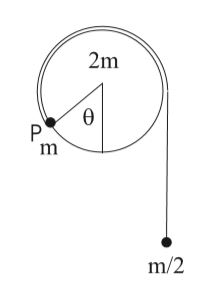
\includegraphics[scale=0.5]{TP1_Q1_L.JPG}
\end{figure}
Write down the Lagrangian for the system in terms of angle of rotation $\theta$ of the disc and the extension $x$ of the string with respect to its natural length. Obtain Lagrange's equation of motion.\\[5pt]
Find the equilibrium position of the disc $\theta_0$ and equilibrium extension $x_0$.\\[5pt]
Show that the natural frequencies $\omega$ of small oscillations of the system are determined by the solution to the equation
$$m^2\omega^4-\bigg(\frac{5k}{2}+\frac{\sqrt{3}mg}{4a}\bigg)m\omega^2+\frac{\sqrt{3}mgk}{2a}=0$$
For the limiting case of a stiff string ($k>>\frac{mg}{a}$), show that the natural frequencies approach $\omega^2=\frac{5k}{2m}$ and $\omega^2=\frac{\sqrt{3}g}{5a}$, and describe the normal modes.\\[5pt]
Find appropriate expressions for the other limiting case $k<<mg/a$ and interpret your results.
\end{qns}
\begin{ans}
Let $x$ is the extension of string with respect to natural length. The kinetic energy is
$$T=\frac{1}{2}\frac{1}{2}(2m)a^2\dot{\theta}^2+\frac{1}{2}ma^2\dot{\theta}^2+\frac{1}{4}m(\dot{x}+a\dot{\theta})^2=\frac{5}{4}ma^2\dot{\theta}^2+\frac{1}{4}m\dot{x}^2+\frac{1}{2}m\dot{x}a\dot{\theta}$$
where the moment of inertia of the disc is $\frac{1}{2}2ma^2$. The potential energy is
$$V=-mga\cos\theta-\frac{1}{2}mg(x+a\theta)+\frac{1}{2}kx^2$$
$$\mathcal{L}=T-V=\frac{5}{4}ma^2\dot{\theta}^2+\frac{1}{4}m\dot{x}^2+\frac{1}{2}m\dot{x}a\dot{\theta}+mga\cos\theta+\frac{1}{2}mg(x+a\theta)-\frac{1}{2}kx^2$$
We have the equations of motion
$$\frac{d}{dt}\frac{\partial\mathcal{L}}{\partial\dot{\theta}}=\frac{d}{dt}(2.5ma^2\dot{\theta}+\frac{1}{2}ma\dot{x})=2.5ma^2\ddot{\theta}+0.5ma\ddot{x},\quad\frac{\partial\mathcal{L}}{\partial\theta}=-mga\sin\theta+\frac{1}{2}mga$$
$$\frac{\partial\mathcal{L}}{\partial x}=0.5mg-kx,\quad\frac{d}{dt}\frac{\partial\mathcal{L}}{\partial\dot{x}}=0.5m\ddot{x}+0.5ma\ddot{\theta}$$
The Lagrange's equations of motion give
\begin{equation}
2.5ma^2\ddot{\theta}+0.5ma\ddot{x}=0.5mga-mga\sin\theta\tag{1a}
\end{equation}
\begin{equation}
0.5mg-kx=0.5m\ddot{x}+0.5ma\ddot{\theta}\tag{1b}
\end{equation}
The equilibrium $\ddot{\theta}=\ddot{x}=0$, so $x_0=\frac{mg}{2k}$ and $\sin\theta_0=0.5\implies\theta_0=\pi/6$.\\[5pt]
Consider small perturbation from equilibrium, i.e. $\theta=\theta_0+\delta\theta$, $x=x_0+\delta x$ and using small angle approximation, 1a and 1b respectively give
$$2.5ma^2\delta\ddot{\theta}+0.5ma\delta\ddot{x}=0.5mga-mga\sin(\theta_0+\delta\theta)\approx0.5mga-mga(0.5+0.5\sqrt{3}\delta\theta)$$
$$0.5mg-kx_0-k\delta x=0.5m\delta\ddot{x}+0.5ma\delta\ddot{\theta}$$
Assume $\delta\theta$ and $\delta x$ vary with time as $e^{i\omega t}$, $\delta\ddot{x}=-\omega^2\delta x$, $\delta\ddot{\theta}=-\omega^2\delta\theta$, so
$$\begin{pmatrix}-0.5m\omega^2+k&-0.5ma\omega^2\\-0.5ma\omega^2&-2.5ma^2\omega^2+0.5\sqrt{3}mga\\\end{pmatrix}\begin{pmatrix}\delta x\\\delta\theta\\\end{pmatrix}=0$$
Setting the determinant to be zero, 
$$0=(-0.5m\omega^2+k)(-2.5ma^2\omega^2+0.5\sqrt{3}mga)-0.25m^2a^2\omega^4=m^2\omega^4-m\omega^2\bigg(2.5k+\frac{\sqrt{3}mg}{4a}\bigg)+\frac{\sqrt{3}mgk}{2a}$$
where $m(\omega_1^2+\omega_2^2)=\frac{5k}{2}+\frac{\sqrt{3}mg}{4a}$, $m^2\omega_1^2\omega_2^2=\frac{\sqrt{3}}{2}\frac{mgk}{a}$. When $k>>mg/a$,
$$m(\omega_1^2+\omega_2^2)\approx2.5k,\quad m^2\omega_1^2\omega_2^2<<1$$
Choose $m\omega_2^2\approx2.5k$, then $m\omega_1^2\approx\frac{\sqrt{3}mgk}{2a}\frac{2}{5k}=\frac{\sqrt{3}mg}{5a}$. When $k<<mg/a$,
$$m(\omega_1^2+\omega_2^2)\approx\frac{\sqrt{3}mg}{4a},\quad m^2\omega_1^2\omega_2^2>>1$$
Choose $m\omega_2^2\approx\frac{\sqrt{3}mg}{4a}$, then $m\omega_1^2\approx\frac{\sqrt{3}mgk}{2a}\frac{4a}{\sqrt{3}mg}=2k$. 
\end{ans}
\begin{qns}
A Lagrangian explicitly dependent on time: the inverted pendulum. The system consists of a bob of mass $m$ at the far end of a light rod of length $l$ whose near end is freely hinged to a support that vibrates vertically with amplitude $a$ and frequency $\frac{\omega}{2\pi}$. Show that
$$\mathcal{L}=\frac{1}{2}m(l^2\dot{\theta}^2+\omega^2a^2\sin^2\omega t+2\omega al\sin\omega t\sin\theta\dot{\theta})-mg(a\cos\omega t+l\cos\theta)$$
where $\theta$ is the inclination to the vertical, and hence that the equation of motion is
$$l^2\ddot{\theta}+\omega^2al\cos\omega t\sin\theta-gl\sin\theta=0$$
\begin{figure}[H]
    \centering
    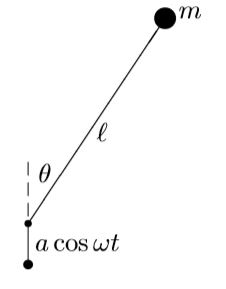
\includegraphics[scale=0.5]{TP1_Q2_L.JPG}
\end{figure}
The motion must consist of a `slow' ($\tau<2\pi\sqrt{l/g}$) motion and a small but forced wobble at frequency $\omega/2\pi>>1/\tau$ (and possibly harmonics). Write
$$\theta=\theta_1+C\cos\omega t+S\sin\omega t$$
where $\theta_1$, $S$ and $C$ vary slowly.\\[5pt]
Substitute this expression into the equation of motion, keeping only first order terms in the small quantities $C$ and $S$. You can then isolate the `slow' terms and those that vary at frequency $\frac{\omega}{2\pi}$; show that the latter obey
$$l^2\ddot{S}-2\omega l^2\dot{C}-\omega^2l^2S-glS\cos\theta_1=0$$
$$l^2\ddot{C}+2\omega l^2\dot{S}-\omega^2l^2C-glC\cos\theta_1=-\omega^2al\sin\theta_1$$
Near an equilibrium value of $\theta_1$, $C$ and $S$ vary arbitrarily slowly, so you can investigate the stability of, and small oscillations about an equilibrium $\theta_1$ neglecting terms in $\dot{C}$ etc. Use the resulting expressions for $C$ and $S$ in the `slow' terms of the equation of motion to show that the upright position of the pendulum is stable iff 
$$\omega^2>\frac{2gl}{a^2}$$
and find the period of small oscillations of $\theta_1$ about zero.
\end{qns}
\begin{ans}
Set the origin such that the position coordinate for the mass $m$ is $x=l\sin\theta$, $y=l\cos\theta+a\cos\omega t$. We thus have $\dot{x}=\dot{\theta}l\cos\theta$ and $\dot{y}=-\dot{\theta}l\sin\theta-a\omega\sin\omega t$. The Lagrangian is 
$$\mathcal{L}=\frac{1}{2}m(\dot{x}^2+\dot{y}^2)-mgy=\frac{1}{2}m(\dot{\theta}^2l^2+a^2\omega^2\sin^2\omega t+2\dot{\theta}la\omega\sin\theta\sin\omega t)-mg(l\cos\theta+a\cos\omega t)$$
The Lagrange equation of motion is
$$\frac{d}{dt}\frac{\partial\mathcal{L}}{\partial\dot{\theta}}=m\ddot{\theta}l^2+mla\omega\cos\theta\dot{\theta}\sin\omega t+mla\omega^2\sin\theta\cos\omega t $$
$$\frac{\partial\mathcal{L}}{\partial\theta}=m\dot{\theta}la\omega \cos\theta\sin\omega t+mgl\sin\theta$$
We thus have
$$0=\frac{d}{dt}\bigg(\frac{\partial\mathcal{L}}{\partial\dot{\theta}}\bigg)-\frac{\partial\mathcal{L}}{\partial\theta}=l^2\ddot{\theta}+a\omega^2l\sin\theta\cos(\omega t)-gl\sin\theta$$
Consider the slow motion $\tau<2\pi\sqrt{l/g}$ but fast small, forced wobble for $\omega/2\pi>>1/\tau$, we write $\theta=\theta_1+C\cos\omega t+S\sin\omega t$,
$$\dot{\theta}=\dot{C}\cos\omega t+\dot{S}\sin\omega t-\omega C\sin\omega t+S\omega \cos\omega t+\dot{\theta}_1$$
$$\ddot{\theta}=\ddot{\theta}_1+\ddot{C}\cos\omega t+\ddot{S}\sin\omega t-2\omega\dot{C}\sin\omega t+2\dot{S}\omega\cos\omega t-\omega^2C\cos\omega t-S\omega^2\sin\omega t$$
We had earlier that
$$l^2\ddot{\theta}+a\omega^2l\sin\theta\cos\omega t-gl\sin\theta=0$$
Using approximation for $\sin\theta=\sin(\theta_1+C\cos\omega t+S\sin\omega t)$:
$$\sin\theta_1\cos(C\cos\omega t+S\sin\omega t)+\cos\theta_1\sin(C\cos\omega t+S\sin\omega t)\approx\sin\theta_1+\cos\theta_1(C\cos\omega t+S\sin\omega t)$$
for small $C,S$. We have $\cos\omega t\sin\theta\approx\cos\omega t\sin\theta_1+C\cos\theta_10.5$ where the half factor is kept from $\cos^2\omega t=0.5(1+\cos(2\omega t))$. Since we are only considering motion that is slowly varying with time, i.e. we keep terms either constant or with frequency $\omega$:
\begin{itemize}
    \item Constant terms:
    \begin{equation}
    l^2\ddot{\theta}_1-gl\sin\theta_1+0.5a\omega^2lC\cos\theta_1=0\tag{2a}
    \end{equation}
    \item $\cos\omega t$ terms:
    \begin{equation}
    l^2(\ddot{C}+2\dot{S}\omega -C\omega^2)+a\omega^2l\sin\theta_1-glC\cos\theta_1=0\tag{2b}
    \end{equation}
    \item $\sin\omega t$ terms:
    \begin{equation}
    l^2(\ddot{S}-2\dot{C}\omega-S\omega^2)-glS\cos\theta_1=0\tag{2c}
    \end{equation}
\end{itemize}
Next, near equilibrium value $\theta_1$, for slowly varying $C$ and $S$, i.e. $\dot{C}=\ddot{C}=0$ and $\dot{S}=\ddot{S}=0$. So 2b and 2c respectively give
$$-Cl^2\omega^2-glC\cos\theta_1=-a^2\omega^2l\sin\theta_1$$
$$-Sl\omega^2-glS\cos\theta_1=0$$
We thus have $S=0$ and $C=\frac{a\omega^2\sin\theta_1}{\omega^2l+g\cos\theta_1}$. For $\omega^2>>g/l$, $C\approx\frac{a\sin\theta_1}{l}$. So, 2a gives
$$0=\ddot{\theta}_1+\sin\theta_1\bigg(-\frac{g}{l}+\frac{a\omega^2}{2l}\frac{a\cos\theta_1}{l}\bigg)$$
When the inverted pendulum is upright, $\theta=0$ and $\cos\theta_1\approx1$ and $\sin\theta_1\approx\theta_1$, then
$$\ddot{\theta}_1+\theta_1\bigg(\frac{a^2\omega^2}{2l^2}-\frac{g}{l}\bigg)=0$$
for this to be a SHM equation, we require $\frac{a^2\omega^2}{2l^2}>\frac{g}{l}\implies\omega^2>\frac{2gl}{a^2}$. The period of small oscillation is
$$T=\frac{2\pi}{\sqrt{\frac{a^2\omega^2}{2l^2}-\frac{g}{l}}}$$
\end{ans}
\newpage
\subsection{Hamilton Formalism}
\subsubsection{Configuration Space and Phase Space}
\begin{defi}[Physical space]
For a system of $N$ particles moving in 3 dimensions without constraints, the physical space in which the particles move is $\mathbb{R}^3$.
\end{defi}
\begin{defi}[Configuration space]
The instantaneous configuration of the system is described by the vectors $\mathbf{r_1},...,\mathbf{r_N}$. If there are no constraints, then the $3N$ components of these vectors are independent, and the configuration space (space of all possible configurations) is $\mathbb{R}^{3N}$. The system is said to have $3N$ degrees of freedom.
\end{defi}
\begin{defi}[Phase space]
The future evolution of the system depends on the positions and the velocities. The $6N$-dimensional vector $(\mathbf{r_1},...,\mathbf{r_N},\mathbf{\dot{r}_1},...,\mathbf{\dot{r}_N})^T$ defines a point in phase space, which here is $\mathbb{R}^{6N}$. The equations of motion define a flow in phase space.
\end{defi}
\begin{eg}
Consider the example of simple harmonic oscillator in 1D, i.e. $\ddot{x}=-x$. The physical space and configuration space are $\mathbb{R}$ while the phase space is $\mathbb{R}^2$. The flow in phase space is clockwise circles, i.e. $\dot{x}=v$ and $\dot{v}=-x$.
\end{eg}
\subsubsection{Legendre Transformation}
\begin{defi}[Legendre transform]
Let $f(x)$ be a convex function of $x$. Let $g(p)$ be the maximum value of $px-f(x)$ with respect to $x$. This defines the Legendre transform $g(p)$ of $f(x)$. The maximum occurs at $x=x^*(p)$ defined by $p=f'(x^*)$. 
\end{defi}
\begin{remarks}
This equation is invertible because the convexity of $f$ implies $f'$ is an increasing function. The Legendre transform is an involution if the Legendre transform of $f$ is $g$, then the Legendre transform of $g$ is $f$.
\end{remarks}
\begin{eg}
Consider for example $f(x)=\frac{1}{2}ax^2$, then $p=f'(x)=ax$ and so $x=\frac{p}{a}$. We have $g(p)=px-f(x)=\frac{1}{2}\frac{p^2}{a}$, i.e. a parabola mapped into a parabola. Another example is $f(x)=e^x$ with $p=e^x\implies x=\ln p$, and so $g(p)=p\ln p-p$.
\end{eg}
\begin{prop}
In terms of differentials, $f(x)$ has the differential $df=pdx$, where $p=\frac{df}{dx}$. Let $g=px-f$ so that
$$dg=pdx+xdp-df=xdp\implies x=\frac{dg}{dp}$$
For functions of several variables, the Legendre transform generates to $g(\mathbf{p})=\mathbf{p}\cdot\mathbf{x}-f(\mathbf{x})$ where $\mathbf{x}$ is determined from $\mathbf{p}$ via $\mathbf{p}=\frac{\partial f}{\partial\mathbf{x}}$, then 
$$dg=\mathbf{p}\cdot d\mathbf{x}+\mathbf{x}\cdot d\mathbf{p}-df=\mathbf{x}\cdot d\mathbf{p}$$
where $df=\mathbf{p}\cdot d\mathbf{x}$. 
\end{prop}
\subsubsection{Hamilton's Equations}
\begin{defi}[Hamiltonian]
The Hamiltonian $\mathcal{H}(\mathbf{q},\mathbf{p},t)$ is defined to be the Legendre transform of the Lagrangian $\mathcal{L}(\mathbf{q},\mathbf{\dot{q}},t)$ with respect to $\mathbf{\dot{q}}$. The variables $\mathbf{q}$ and $t$ are passive in the Legendre transform. Thus, $\mathcal{H}=\mathbf{p}\cdot\mathbf{\dot{q}}-\mathcal{L}$ with $\mathbf{p}=\frac{\partial\mathcal{L}}{\partial\mathbf{\dot{q}}}$. 
\end{defi}
It is important that $\mathbf{\dot{q}}$ is to be eliminated in favour of $\mathbf{p}$. 
\begin{prop}[Hamilton's equations]
$$\frac{\partial\mathcal{H}}{\partial\mathbf{p}}=\mathbf{\dot{q}},\quad\frac{\partial\mathcal{H}}{\partial\mathbf{q}}=-\mathbf{\dot{p}},\quad\frac{\partial\mathcal{H}}{\partial t}=-\frac{\partial\mathcal{L}}{\partial t}$$
\end{prop}
\begin{proof}
The total differential of $\mathcal{H}$ is
$$d\mathcal{H}=\mathbf{p}\cdot d\mathbf{\dot{q}}+\mathbf{\dot{q}}\cdot d\mathbf{p}-d\mathcal{L}=\mathbf{\dot{q}}\cdot d\mathbf{p}-\mathbf{\dot{p}}\cdot d\mathbf{q}-\frac{\partial\mathcal{L}}{\partial t}dt$$
where $\mathbf{\dot{p}}=\frac{\partial\mathcal{L}}{\partial\mathbf{q}}$ from Lagrange's equations since $\mathbf{p}=\frac{\partial\mathcal{L}}{\partial\mathbf{\dot{q}}}$. To get the Hamilton's equations, compare this with the expression $$d\mathcal{H}=\frac{\partial\mathcal{H}}{\partial\mathbf{q}}\cdot d\mathbf{q}+\frac{\partial\mathcal{H}}{\partial\mathbf{p}}\cdot d\mathbf{p}+\frac{\partial\mathcal{H}}{\partial t}dt$$
\end{proof}
\begin{remarks}
For a system with $n$ degrees of freedom, we obtain $2n$ first-order DEs instead of $n$ second-order DEs (like in Lagrangian dynamics). $\mathbf{p}$ is thought of as an independent variables from $\mathbf{q}$ on an equal footing (treated almost symmetrically).
\end{remarks}
\begin{prop}
Hamilton's equations define a flow in phase space $\mathbf{r}=(\mathbf{q},\mathbf{p})$. The flow is orthogonal to the gradient of $\mathcal{H}$. For an autonomous system for which $\mathcal{L}$ and $\mathcal{H}$ do not depend explicitly on $t$, we have $\mathcal{H}$ being constant along the path in phase space, $\mathcal{H}$ can often be identified with the energy of the system.
\end{prop}
\begin{proof}
The time evolution of the phase space is given by the Hamilton's equations, and is indeed orthogonal to the gradient of $\mathcal{H}$:
$$\mathbf{\dot{r}}=\begin{pmatrix}\dot{\mathbf{q}}\\\dot{\mathbf{p}}\\\end{pmatrix}=\begin{pmatrix}\frac{\partial\mathcal{H}}{\partial\mathbf{p}}\\-\frac{\partial\mathcal{H}}{\partial\mathbf{q}}\\\end{pmatrix},\quad\boldsymbol{\nabla}\mathcal{H}=\begin{pmatrix}\frac{\partial\mathcal{H}}{\partial\mathbf{q}}\\\frac{\partial\mathcal{H}}{\partial\mathbf{p}}\\\end{pmatrix},\quad\boldsymbol{\nabla}\mathcal{H}\cdot\mathbf{\dot{r}}=\frac{\partial\mathcal{H}}{\partial\mathbf{q}}\cdot\frac{\partial\mathcal{H}}{\partial\mathbf{p}}-\frac{\partial\mathcal{H}}{\partial\mathbf{q}}\cdot\frac{\partial\mathcal{H}}{\partial\mathbf{p}}=0$$
$$\frac{d\mathcal{H}}{dt}=\frac{\partial\mathcal{H}}{\partial\mathbf{p}}\cdot\mathbf{\dot{p}}+\frac{\partial\mathcal{H}}{\partial\mathbf{q}}\cdot\mathbf{\dot{q}}+\frac{\partial\mathcal{H}}{\partial t}=\frac{\partial\mathcal{H}}{\partial\mathbf{p}}\cdot\bigg(-\frac{\partial\mathcal{H}}{\partial\mathbf{q}}\bigg)+\frac{\partial\mathcal{H}}{\partial\mathbf{q}}\cdot\frac{\partial\mathcal{H}}{\partial\mathbf{p}}+0=0$$
Finally, when $\mathcal{H}$ is time independent ($\frac{\partial\mathcal{H}}{\partial t}=0$), then $\mathcal{H}$ is constant.
\end{proof}
\begin{eg}
For a particle in 1D potential, we have $\mathcal{L}=\frac{1}{2}m\dot{x}^2-V(x)$. Set $q=x$, $p=m\dot{x}$ and so $\mathcal{H}(x,p)=p\dot{q}-\mathcal{L}=\frac{1}{2}m\dot{x}^2+V(x)=\frac{p^2}{2m}+V(x)$ is the total energy. Quadratic functions are mapped to quadratic functions, as expected. The Hamilton's equations are $\dot{q}=\frac{\partial\mathcal{H}}{\partial p}\implies\dot{x}=\frac{p}{m}$, $\dot{p}=-\frac{\partial\mathcal{H}}{\partial q}\implies\dot{p}=-V'(x)$.
\end{eg}
\begin{defi}[Representative Point]
A representative point is a single point in phase space represents the state of the whole system. In presence of the constraints, these points are confined to some lower dimensional subspace. We regard the initial state of ensemble of systems as corresponding to a density of representative points in phase space.
\end{defi}
\begin{prop}
The action integral is stationary with respect to the variations in which $\mathbf{q}$ iff the Hamilton's equations $\mathbf{\dot{q}}=\frac{\partial\mathcal{H}}{\partial\mathbf{p}}$ and $\mathbf{\dot{p}}=-\frac{\partial\mathcal{H}}{\partial\mathbf{q}}$ are both satisfied.
\end{prop}
\begin{proof}
We obtained $\mathcal{H}$ from $\mathcal{L}$ via Legendre’s transformation $\mathcal{H}=\mathbf{p}\cdot\mathbf{\dot{q}}-\mathcal{L}$. The action integral is then $S=\int_{t_1}^{t_2}\mathcal{L}dt=\int_{t_1}^{t_2}(\mathbf{p}\cdot\mathbf{\dot{q}}-\mathcal{H})dt$. Consider the variation of $S$ under independent variations of $q$ and $p$:
$$0=\delta S=\int_{t_1}^{t_2}\bigg(\mathbf{p}\cdot\delta\mathbf{\dot{q}}+\mathbf{\dot{q}}\cdot\delta\mathbf{p}-\frac{\partial\mathcal{H}}{\partial\mathbf{q}}\cdot\delta\mathbf{q}-\frac{\partial\mathcal{H}}{\partial\mathbf{p}}\cdot\delta\mathbf{p}\bigg)dt=[\mathbf{p}\cdot\delta\mathbf{q}]_{t_1}^{t_2}+\int_{t_1}^{t_2}\bigg(-\bigg(\mathbf{\dot{p}}+\frac{\partial\mathcal{H}}{\partial\mathbf{q}}\bigg)\cdot\delta\mathbf{q}+\bigg(\mathbf{\dot{q}}-\frac{\partial\mathcal{H}}{\partial\mathbf{p}}\bigg)\cdot\delta\mathbf{p}\bigg)dt$$
where we integrated by parts.
\end{proof}
\begin{prop}
 For a time-independent Hamiltonian, the action (also called `abbreviated action') depends strictly on the path taken in phase space and not on the rate at which the path is traversed.
\end{prop}
\begin{proof}
 If $\mathcal{H}$ does not depends explicitly on $t$, then it is conserved and the action is $S=\int_{t_1}^{t_2}\mathbf{p}\cdot d\mathbf{q}-H\int_{t_1}^{t_2}dt$. The last term can be ignore because it is independent of the path. The first term is called `abbreviated action', which depends strictly on path taken in phase space (not on rate at which path is traversed). Action path taken makes this line integral stationary.
\end{proof}
\begin{thm}[Liouville's theorem]
The phase-space density is conserved following the flow in phase space. 
\end{thm}
\begin{proof}
Consider an ensemble consisting of a large number of systems with the same Hamiltonian function but different initial conditions. Each is represented by a `particle' following the flow in phase space. If they are closely spaced, we can discuss their phase-space density $\rho(\mathbf{q},\mathbf{p},t)$. Since the particles are conserved, $\rho$ satisfies the conservation equation $\frac{\partial\rho}{\partial t}+\boldsymbol{\nabla}\cdot(\rho\mathbf{v})=0$. But the Hamiltonian flow satisfies $\boldsymbol{\nabla}\cdot\mathbf{v}=\frac{\partial}{\partial q_i}\frac{\partial H}{\partial p_i}-\frac{\partial}{\partial p_i}\frac{\partial H}{\partial q_i}=0$, so
$$\frac{D\rho}{Dt}:=\frac{\partial\rho}{\partial t}+\mathbf{v}\cdot\boldsymbol{\nabla}\rho=\frac{\partial\rho}{\partial t}+\boldsymbol{\nabla}\cdot(\rho\mathbf{v})-\rho\boldsymbol{\nabla}\cdot\mathbf{v}=0$$
i.e. $\rho$ is thus conserved along a streamline (Hamiltonian).
\end{proof}
\begin{remarks}
The theorem states that the density in phase space evolves as an incompressible fluid. In another words, the volume occupied by ensemble's representative points do not change. Equilibrium (time-independent) solutions for the phase-space density are possible if $\rho$ is a function of the integrals of motion. 
\end{remarks}
\subsubsection{Poisson Brackets}
\begin{defi}[Poisson bracket]
The Poisson bracket of two functions $f(\mathbf{q}, \mathbf{p}, t)$ and $g(\mathbf{q}, \mathbf{p}, t)$ is defined as
$$\{f,g\}:=\frac{\partial f}{\partial\mathbf{q}}\cdot\frac{\partial g}{\partial\mathbf{p}}-\frac{\partial g}{\partial\mathbf{q}}\cdot\frac{\partial f}{\partial\mathbf{p}}=\sum_{i=1}^n\bigg(\frac{\partial f}{\partial q_i}\frac{\partial g}{\partial p_i}-\frac{\partial f}{\partial p_i}\frac{\partial g}{\partial q_i}\bigg)$$
Essentially, this is an antisymmetric product of partial derivatives of $f$ and $g$.
\end{defi}
\begin{prop}
The Poisson bracket has the following properties,  where  $f$, $g$, $h$ are functions, and $\alpha$, $\beta$ are constant):
\begin{enumerate}
    \item Anti-symmetry, i.e. $\{f,g\}=-\{g,f\}$
    \item Linearity, i.e. $\{\alpha f+\beta g,h\}=\alpha\{f,h\}+\beta\{g,h\}$
    \item Leibniz rule, i.e. $\{fg,h\}=f\{g,h\}+\{f,h\}g$ (from product rule of differentiation)
    \item Jacobi identity, i.e. $\{f,\{g,h\}\}+\{g,\{h,f\}\}+\{h,\{f,g\}\}=0$.
\end{enumerate}
Clearly $\{f, f\} = 0$ and $\{f, c\} = 0$ where $c$ is constant. Two functions whose Poisson bracket vanish are said to Poisson-commute.
\end{prop}
\begin{defi}[Canonical commutation relations]
The Poisson bracket of the canonical variables $\mathbf{q}$ and $\mathbf{p}$ are
$$\{q_i,q_j\}=0,\quad\{p_i,p_j\}=0,\quad\{q_i,p_j\}=\delta_{ij}$$
these are called the canonical commutation relations.  
\end{defi}
\begin{prop}[Hamilton's equations in Poisson bracket form]
Any function $f(\mathbf{q}, \mathbf{p}, t)$ such that $\frac{\partial f}{\partial t}=0$ is a conserved quantity or constant of the motion. So any function $f(\mathbf{q}, \mathbf{p})$ that Poisson-commutes with $\mathcal{H}$ is a conserved quantity, called (first) integral of motion. 
\end{prop}
\begin{proof}
The time-evolution of any function $f(\mathbf{q}, \mathbf{p}, t)$ is given by
$$\frac{df}{dt}=\frac{\partial f}{\partial\mathbf{q}}\cdot\mathbf{\dot{q}}+\frac{\partial f}{\partial\mathbf{p}}\cdot\mathbf{\dot{p}}+\frac{\partial f}{\partial t}=\frac{\partial f}{\partial\mathbf{q}}\cdot\frac{\partial\mathcal{H}}{\partial\mathbf{p}}-\frac{\partial f}{\partial\mathbf{p}}\cdot\frac{\partial\mathcal{H}}{\partial\mathbf{q}}+\frac{\partial f}{\partial t}=\{f,H\}+\frac{\partial f}{\partial t}$$
\end{proof}
\begin{remarks}
$\mathcal{H}$ is a conserved quantity if $\frac{\partial\mathcal{H}}{\partial t}=0$. $p_i$ is conserved if $\frac{\partial\mathcal{H}}{\partial q_i}=0$.
\end{remarks}
\begin{thm}[Poisson theorem]
The Poisson bracket of two conserved quantities is also a conserved quantity.
\end{thm}
\begin{proof}
Follows quickly from Jacobi identity if functions don’t functions don’t depends explicitly on $t$. More generally, for time dependent functions:
$$\frac{d}{dt}\{f, g\} =\{\{f, g\}, H\} +\frac{\partial}{\partial t}\{f, g\}=\{f, \{g, H\}\} + \{\{f, H\}, g\} + \{\dot{f},g\}+\{f, \dot{g}\}=\{f,\dot{g}\}+\{\dot{f},g\}=0$$
\end{proof}
\begin{defi}[Canonical transformation]
Consider a change of variables in phase space from $(\mathbf{q},\mathbf{p})$ to $(\mathbf{Q},\mathbf{P})$ where $\mathbf{Q}$ and $\mathbf{P}$ are functions $(\mathbf{q},\mathbf{p}, t)$. This transformation is said to be canonical if it preserves the form of Hamilton’s equation, i.e.
$$\mathbf{\dot{Q}}=\frac{\partial K}{\partial\mathbf{P}},\quad\mathbf{\dot{P}}=-\frac{\partial K}{\partial\mathbf{Q}}$$
where $K(\mathbf{Q},\mathbf{P},t)$ is a new Hamiltonian.
\end{defi}
\begin{prop}
 The transformation is canonical iff the new variables satisfy the canonical commutation relations.
 $$\{Q_i,Q_j\}=0,\quad\{P_i,P_j\}=0,\quad\{Q_i,P_j\}=\delta_{ij}$$
\end{prop}
\begin{prop}
Poisson bracket is invariant under a canonical transformation.
\end{prop}
\begin{remarks}[Action-angle variables]
In general, the canonical transformation must satisfy the canonical commutation relations and will always keep the Poisson bracket invariant.\\[5pt]
For an autonomous system with $n=1$, $\dot{q}=\frac{\partial H}{\partial p}$ and $\dot{p}=-\frac{\partial H}{\partial q}$ are the Hamilton's equations. We aim to make a canonical transformation $(q,p)\mapsto(Q,P)$ such that $H(Q,P)=H(P)$ depends only on $P$. In this case, the Hamilton's equations will take the simple form
$$\dot{P}=0\implies P=\text{const},\quad\dot{Q}=\frac{dH}{dP}=\text{const}$$
In fact, we know $H$ is constant, so $P$ could be any function of $H$.\\[5pt]
In particular, we can relabel $(Q,P)$ as $(\theta,I)$, the action-angle variables, where $\theta$ is the angle and $I=\frac{1}{2\pi}\oint pdq$ is the action. The Hamilton's equations in action-angle variables reduce to 
$$\dot{\theta}=\frac{dH}{dI},\quad\dot{I}=0$$
with $\omega(I)=\frac{dH}{dI}$ being the angular frequency of the orbit.
\end{remarks}
\begin{remarks}[Generating function]
Generating functions provide a practical way to find canonical transformations. Let $(\mathbf{q},\mathbf{p})$ be canonical variables with Hamiltonian $H$. If the new variables $(\mathbf{Q},\mathbf{P})$ are also canonical with Hamiltonian $K$, then we must have
$$\delta\bigg[\int(\mathbf{p}\cdot d\mathbf{q}-Hdt)\bigg]=0\implies\delta\bigg[\int(\mathbf{P}\cdot d\mathbf{Q}-Kdt)\bigg]=0$$
These two forms are equivalent if the integrands differ by a total differential, i.e. $\mathbf{p}\cdot d\mathbf{q}-Hdt=\mathbf{P}\cdot d\mathbf{Q}-Kdt+dF$. In this case, $F$ is called the generating function of the canonical transformation. $F$ always satisfy
$$\frac{dF}{dt}=\mathcal{L}(\mathbf{q},\mathbf{p},t)-\mathcal{L}(\mathbf{Q},\mathbf{P},t),\quad\frac{\partial F}{\partial t}=K(\mathbf{Q},\mathbf{P},t)-H(\mathbf{q},\mathbf{p},t)$$
\end{remarks}
\begin{eg}\leavevmode
\begin{itemize}
    \item If $F_2=\mathbf{q}\cdot\mathbf{P}$, then $\mathbf{p}=\mathbf{P}$, $\mathbf{Q}=\mathbf{q}$, $K=H$. This is the trivial identity transformation;
    \item If $F_1=\mathbf{q}\cdot\mathbf{Q}$, then $\mathbf{p}=\mathbf{Q}$, $\mathbf{Q}=-\mathbf{P}$, $K=H$. The coordinates and momenta are interchanged (with some sign changes).
    \item Consider the generating function $F_1=\frac{1}{2}q^2\cot Q$. We obtain $p=\frac{\partial F_1}{\partial q}=q\cot Q$, $P=-\frac{\partial F_1}{\partial Q}=\frac{1}{2}q^2\cosec^2Q$, so $P=\frac{1}{2}(p^2+q^2)$ and $Q=\tan^{-1}(q/p)$ with inverse relation $q=\sqrt{2P}\sin(Q)$ and $p=\sqrt{2P}\cos(Q)$. This transformation mixes coordinates and momenta. This is also similar to transformation from rectangular to polar coordinates.
\end{itemize}
\end{eg}
\newpage
\subsubsection{Relation to Quantum Mechanics}
\subsubsection*{Commutators and Poisson Brackets}
In Quantum Mechanics, the commutator of two operators (which represent observables) is defined as $[A,B]=AB-BA$. The canonical commutation relations are highly reminiscent of Poisson Brackets, with $[A,B]\sim i\hbar\{A,B\}$.\\[5pt] 
In the Heisenberg picture, the quantum state $|\psi\rangle$ is time-independent but the operator $A$ evolves as
$$\frac{dA}{dt}=\frac{1}{i\hbar}[A,H]+\frac{\partial A}{\partial t}$$
reminiscent to $\frac{df}{dt}=\{f,H\}+\frac{\partial f}{\partial t}$.
\subsubsection*{Hamilton-Jacobi and Schr\"{o}dinger Equations}
Suppose that $F_2(\mathbf{q},\mathbf{P},t)$ is the generating function of a canonical transformation $(\mathbf{q},\mathbf{p})\mapsto(\mathbf{Q},\mathbf{P})$ such that the new Hamiltonian vanishes, $K=H+\frac{\partial F_2}{\partial t}=0$. Then $\mathbf{p}=\frac{\partial F_2}{\partial\mathbf{q}}$ and $\mathbf{Q}=\frac{\partial F_2}{\partial\mathbf{P}}$. We have
$$\frac{dF_2}{dt}=\frac{\partial F_2}{\partial\mathbf{q}}\cdot\mathbf{\dot{q}}+\frac{\partial F_2}{\partial\mathbf{P}}\cdot\mathbf{P}+\frac{\partial F_2}{\partial t}=\mathbf{p}\cdot\mathbf{\dot{q}}-H=\mathcal{L}$$
where $\mathcal{L}$ is the Lagrangian. Hence, $F_2=S(q,t)=\int \mathcal{L}dt$ is the action, considered as an indefinite integral from some initial configuration to the current configuration $(\mathbf{q},t)$ along the physical path.\\[5pt]
$S(\mathbf{q},t)$ is known as the Hamilton's characteristic function. Given a Hamiltonian function $H(\mathbf{q},\mathbf{p},t)$, $S$ satisfies the Hamilton-Jacobi equation $\frac{\partial S}{\partial t}=H(\mathbf{q},\frac{\partial S}{\partial\mathbf{q}},t)$ which is a first-order non-linear PDE for $S(\mathbf{q},t)$. An important example is $H=\frac{|\mathbf{p}|^2}{2m}+V(\mathbf{r})$ in which case we have
$$\frac{\partial S}{\partial t}=\frac{|\boldsymbol{\nabla}S|^2}{2m}+V(\mathbf{r})$$
which is highly reminiscent to the Schr\"{o}dinger equation $i\hbar\frac{\partial\psi}{\partial t}=-\frac{\hbar^2}{2m}\nabla^2\psi+V(\mathbf{r})\psi$ for the wavefunction $\psi(\mathbf{r},t)$. Let $\psi=Re^{iS/\hbar}$ where $R(\mathbf{r},t)$ and $S(\mathbf{r},t)$ are real, then we have
$$\frac{\partial S}{\partial t}=\frac{|\boldsymbol{\nabla}S|^2}{2m}+V(\mathbf{r})-\frac{\hbar^2}{2m}\frac{\nabla^2R}{R}$$
where the last term is a quantum correction. This motivates a form $\psi=C\int e^{iS[\mathbf{q}]/\hbar}D\mathbf{q}$ (a functional integral), related to the Feynmann path integral.
\subsubsection*{Path Integral}
In quantum mechanics, we associate a wavevector $\mathbf{k} = \mathbf{p}/\hbar$ with a particle of momentum $\mathbf{p}$ (de Broglie relation), and frequency $\omega=H/\hbar$ with its total energy $E = H$ (Planck-Einstein relation). Thus we can write Hamilton’s principle for the classical motion of the particle as
$$\frac{1}{\hbar}\int \mathcal{L}dt=\int(\mathbf{p}\cdot\mathbf{\dot{q}}/\hbar-H/\hbar)dt=\int(\mathbf{k}\cdot d\mathbf{q}-\omega dt)=\text{stationary}$$
i.e. the wave-mechanical phase shall be stationary. This is the condition for constructive interference of waves, i.e. the particle goes where the relevant de Broglie waves reinforce. If we move a little away from the classical path, the waves do not reinforce so much and the particle is less likely to be found there. If we imagine taking the limit $\hbar\rightarrow0$, the wavefunction falls off so rapidly away from the classical path that the particle will never deviate from it.\\[5pt]
We see that classical mechanics is the `geometrical optics' limit of QM: the `rays' correspond to the classical paths and quantum effects (like diffraction) are due to the finite frequency and wave number of waves of given energy and momentum, i.e the non-zero value of $\hbar$.
\newpage
\subsubsection{Problems}
\begin{qns}
A particle of mass $m$ moves in a potential $V=\frac{1}{2}kr^2$ (2D Harmonic Oscillator). Find its Hamiltonian using a generalized coordinates $q_1=r$ and $q_2=mr^2\dot{\theta}$ (its angular momentum about the origin), and their conjugate `momenta'. It is easy if you begin with the more natural choice $q_1=r$, $q_2=\theta$ and then interchange the notations for $p_2$ and $-q_2$ when you have reached the Hamiltonian.\\[5pt]
Verify that Hamilton's equations give the expected motion. Notice that this goes sour if you write the Lagrangian $\mathcal{L}$ in terms of $q_1$, $\dot{q}_1$, $q_2$, $\dot{q}_2$ and try to define $p_1=\frac{\partial\mathcal{L}}{\partial\dot{q}_1}$, $p_2=\frac{\partial\mathcal{L}}{\partial\dot{q}_2}$, $H=\mathbf{p}\cdot\mathbf{\dot{q}}-\mathcal{L}$. That happens because the Lagrangian formulation depends on the $q$ really being position coordinates.
\end{qns}
\begin{ans}
We have the Lagrangian to be
$$\mathcal{L}=\frac{1}{2}m(\dot{r}^2+r^2\dot{\theta}^2)-\frac{1}{2}kr^2,\quad p_r=\frac{\partial\mathcal{L}}{\partial\dot{r}}=m\dot{r},\quad p_\theta=\frac{\partial\mathcal{L}}{\partial\dot{\theta}}=mr^2\dot{\theta}$$
Then, it follows that the Hamiltonian will be 
$$H=p_r\dot{r}+p_\theta\dot{\theta}-\mathcal{L}=\frac{1}{2}m(\dot{r}^2+r^2\dot{\theta}^2)-\frac{1}{2}kr^2=\frac{1}{2m}(p_r^2+\frac{p_\theta^2}{r^2})+\frac{1}{2}kr^2$$
We change the notation to the given generalized coordinates:
$$p_r\rightarrow p_1,\quad r\rightarrow q_1,\quad p_\theta\rightarrow q_2,\quad\theta\rightarrow -p_2$$
Hence, the Hamiltonian is $H=\frac{1}{2m}(p_1^2+\frac{q_2^2}{q_1^2})+\frac{1}{2}kq_1^2$. The Hamilton's equations give
$$\dot{p}_1=-\frac{\partial H}{\partial q_1}=-kq_1+\frac{1}{m}\frac{q_2^2}{q_1^3}=-kr+\frac{p_\theta^3}{mr^3}\implies m\ddot{r}=\frac{(mr^2)^2\dot{\theta}^2}{mr^3}-kr=mr\dot{\theta}^2-kr$$
which gives the desired radial equation of motion, i.e. the rate of change of radial momentum is the centrifugal term and that due to the central potential.
$$\dot{p}_2=-\frac{\partial H}{\partial q_2}=-\frac{q_2}{mq_1^2}=-\frac{mr^2\dot{\theta}}{mr^2}=-\dot{\theta},\quad\dot{q}_1=\frac{\partial H}{\partial p_1}=\frac{p_1}{m}=\dot{r}$$
which gives back our substitution. Finally,
$$\dot{q}_2=\frac{\partial H}{\partial p_2}=0\implies\dot{p}_\theta=0$$
which is expected since angular momentum is conserved for any central potential.
\end{ans}
\begin{qns}
What are the main advantages of the Hamiltonian formulation of mechanics over the Lagrangian formulation?\\[5pt]
Derive Hamilton's equations of motion for the one-dimensional Hamiltonian $H(q,p)=p\dot{q}-L(q,\dot{q})$.\\[5pt]
If the Hamiltonian is written in terms of transformed position and momentum coordinates $Q=Q(q,p)$, $P=P(q,p)$, show that the transformed Hamiltonian $H(Q,P)$ obeys Hamilton's equations of motion in the new coordinates only if $\{Q,P\}_{q,p}=1$, where the Poisson bracket is defined by
$$\{U,V\}_{q,p}=\frac{\partial U}{\partial q}\frac{\partial V}{\partial p}-\frac{\partial U}{\partial p}\frac{\partial V}{\partial q}$$
Show that for the coordinate transformations $Q=\tan^{-1}(m\omega q/p)$ and $P=\frac{1}{2m\omega}(p^2+m^2\omega^2q^2)$, the above Poisson bracket holds.\\[5pt]
Rewrite the one-dimensional harmonic oscillator Hamiltonian
$$H=\frac{p^2}{2m}+\frac{1}{2}m\omega^2q^2$$
in terms of $Q$, $P$ and solve the Hamilton's equations in these coordinates. Show that your solutions are consistent with the solutions to the harmonic oscillator solved using $q$, $p$.
\end{qns}
\begin{ans}
The advantages of Hamilton formulation are:
\begin{itemize}
    \item This leads to $2N$ first order DEs instead of $N$ second order DEs, hence easier to solve.
    \item $q_i$ and $p_i$ are now on equal footing such that $q_i$ need not be position coordinates. Canonical transformations with mixed momenta and positions greatly simplify Hamilton's equations.
    \item This is much easier to identify constants of motion. Presence of a conserved quantity immediately simplifies Hamilton's equations.
    \item Simple relationships between classical Hamiltonian formulation and Quantum Mechanics. 
\end{itemize}
Recall $H(q,p,t)=p\dot{q}-\mathcal{L}(q,\dot{q},t)$, we have
$$dH=pd\dot{q}+\dot{q}dp-\frac{\partial\mathcal{L}}{\partial q}dq-\frac{\partial\mathcal{L}}{\partial\dot{q}}d\dot{q}-\frac{\partial\mathcal{L}}{\partial t}dt=\dot{q}dp-\dot{p}dq-\frac{\partial\mathcal{L}}{\partial t}dt$$
where $\dot{p}=\frac{d}{dt}\frac{\partial\mathcal{L}}{\partial\dot{q}}=\frac{\partial\mathcal{L}}{\partial q}$. By comparing with the chain rule, $dH=\frac{\partial H}{\partial p}dp+\frac{\partial H}{\partial q}dq+\frac{\partial H}{\partial t}dt$, the Hamilton's equations of motion are
$$\dot{q}=\frac{\partial H}{\partial p},\quad\dot{p}=-\frac{\partial H}{\partial q},\quad\frac{\partial H}{\partial t}=-\frac{\partial\mathcal{L}}{\partial t}\implies\begin{pmatrix}\dot{q}\\\dot{p}\\\end{pmatrix}=\begin{pmatrix}0&1\\-1&0\\\end{pmatrix}\begin{pmatrix}\frac{\partial H}{\partial q}\\\frac{\partial H}{\partial p}\\\end{pmatrix}$$
We now perform a canonical transformation. By chain rule,
$$\begin{pmatrix}\frac{\partial H}{\partial q}\\\frac{\partial H}{\partial p}\\\end{pmatrix}=\begin{pmatrix}\frac{\partial Q}{\partial q}&\frac{\partial P}{\partial q}\\\frac{\partial Q}{\partial p}&\frac{\partial P}{\partial p}\\\end{pmatrix}\begin{pmatrix}\frac{\partial H}{\partial Q}\\\frac{\partial H}{\partial P}\\\end{pmatrix}\implies\begin{pmatrix}\dot{Q}\\\dot{P}\\\end{pmatrix}=\begin{pmatrix}\frac{\partial Q}{\partial q}&\frac{\partial Q}{\partial p}\\\frac{\partial P}{\partial q}&\frac{\partial P}{\partial p}\\\end{pmatrix}\begin{pmatrix}\dot{q}\\\dot{p}\\\end{pmatrix}=\begin{pmatrix}\frac{\partial Q}{\partial q}&\frac{\partial Q}{\partial p}\\\frac{\partial P}{\partial q}&\frac{\partial P}{\partial p}\\\end{pmatrix}\begin{pmatrix}0&1\\-1&0\\\end{pmatrix}\begin{pmatrix}\frac{\partial Q}{\partial q}&\frac{\partial P}{\partial q}\\\frac{\partial Q}{\partial p}&\frac{\partial P}{\partial p}\\\end{pmatrix}\begin{pmatrix}\frac{\partial H}{\partial Q}\\\frac{\partial H}{\partial P}\\\end{pmatrix}$$
For the Hamilton's equations to be obeyed in $(Q,P)$, then the following is true:
$$\begin{pmatrix}\dot{Q}\\\dot{P}\\\end{pmatrix}=\begin{pmatrix}0&1\\-1&0\\\end{pmatrix}\begin{pmatrix}\frac{\partial H}{\partial Q}\\\frac{\partial H}{\partial P}\\\end{pmatrix}$$
Hence, we must have:
$$\begin{pmatrix}0&1\\-1&0\\\end{pmatrix}=\begin{pmatrix}-\frac{\partial Q}{\partial p}&\frac{\partial Q}{\partial q}\\-\frac{\partial P}{\partial p}&\frac{\partial P}{\partial q}\\\end{pmatrix}\begin{pmatrix}\frac{\partial Q}{\partial q}&\frac{\partial P}{\partial q}\\\frac{\partial Q}{\partial p}&\frac{\partial P}{\partial p}\\\end{pmatrix}$$
The (2,1) element gives $-1=-\frac{\partial P}{\partial p}\frac{\partial Q}{\partial q}+\frac{\partial P}{\partial q}\frac{\partial Q}{\partial p}=-\{Q,P\}_{q,p}$, i.e. the new variables $(Q,P)$ satisfy the canonical commutation relations, if $H(Q,P)$ obeys the Hamilton's equations of motion. In fact, this is a canonical transformation.\\[5pt]
For the given $Q=\tan^{-1}(m\omega q/p)$, $P=\frac{1}{2m\omega}(p^2+m^2\omega^2q^2)$, we have
$$\frac{\partial Q}{\partial q}=\frac{m\omega p}{p^2+(m\omega q)^2},\quad\frac{\partial Q}{\partial p}=-\frac{m\omega q}{p^2+(m\omega q)^2},\quad\frac{\partial P}{\partial q}=m\omega q,\quad\frac{\partial P}{\partial p}=\frac{p}{m\omega}$$
$$\{Q,P\}_{q,p}=\frac{\partial P}{\partial p}\frac{\partial Q}{\partial q}-\frac{\partial P}{\partial q}\frac{\partial Q}{\partial p}=\frac{p}{m\omega}\frac{m\omega p}{p^2+(m\omega q)^2}-\frac{m\omega q(-m\omega q)}{p^2+(m\omega q)^2}=1$$
For the 1D harmonic oscillator,
$$H=\frac{p^2}{2m}+\frac{1}{2}m\omega^2q^2=\frac{2m\omega P}{2m}\cos^2Q+\frac{1}{2}m\omega^2\frac{2m\omega P}{m^2\omega^2}\sin^2Q=\omega P$$
where $\cos Q=\frac{p}{\sqrt{2m\omega P}}$. Hence,
$$\dot{Q}=\frac{\partial H}{\partial P}=\omega\implies Q=\omega t+\alpha,\quad-\dot{P}=\frac{\partial H}{\partial Q}=0\implies P=\beta$$
for some constants $\alpha$, $\beta$. This is an example of an action-angle variable. Then, $p=\sqrt{2m\omega\beta}\cos(\omega t+\alpha)$, $q=\frac{\sqrt{2m\omega\beta}}{m\omega}\sin(\omega t+\alpha)$. This has the form similar to the familiar solution for our harmonic oscillator.
\end{ans}
\begin{qns}
Show that, if we have velocity-dependent potentials that depend only linearly on the velocities, i.e. $V(\mathbf{q},\mathbf{\dot{q}})=V_1(\mathbf{q})+\sum_ia_i(\mathbf{q})\dot{q}_i$, then the quantity
$$H=\sum_i\dot{q}_i\frac{\partial\mathcal{L}}{\partial\dot{q}_i}-\mathcal{L}=T+V_1$$
Explain why this does not mean that the velocity-dependent part of the potential has no effect on the Hamilton's equations of motion.
\end{qns}
\begin{ans}
We have $p_i=\frac{\partial\mathcal{L}}{\partial\dot{q}_i}=\frac{\partial T}{\partial\dot{q}_i}-a_i$ and so $\dot{q}_ip_i=2T-a_i\dot{q}_i$, assuming $T=k_i\dot{q}_i^2$ for some $k_i$. Hence, the Hamiltonian is
$$H=\sum_i\dot{q}_ip_i-\mathcal{L}=2T-\sum_i a_i\dot{q}_i-T+V=T+V_1$$
In another words, the total energy can simply be obtained by measuring the kinetic energy $T$, and the position-dependent part of the potential $V_1(\mathbf{q})$.\\[5pt]
The velocity-dependent part of the potential explicitly appears in Hamiltonian formulation through the change of variable from $\mathbf{\dot{q}}$ to conjugate momenta $\mathbf{p}$.
\end{ans}
\begin{qns}
It is very easy to demonstrate relations between symmetries of the Hamiltonian and conservation laws, e.g.
$$\frac{dH}{dt}=\sum\frac{\partial H}{\partial p_i}\dot{p}_i+\sum\frac{\partial H}{\partial q_i}\dot{q}_i+\frac{\partial H}{\partial t}=\mathbf{\dot{q}}\cdot\mathbf{\dot{p}}-\mathbf{\dot{p}}\cdot\mathbf{\dot{q}}+\frac{\partial H}{\partial t}=0$$
if the Hamiltonian does not depend explicitly on time. Show that, if the Hamiltonian is invariant under a displacement $\delta x$ of the whole system, then $\sum p_x$ is conserved.
\end{qns}
\begin{ans}
Consider $x\rightarrow x+\delta x$, then $H\mapsto H+\delta H$. Suppose $\delta H=0$ (invariant under translation), but $\delta H=\sum\delta x\frac{\partial H}{\partial x}=-\sum\dot{p}\delta x$. For non-zero arbitrary infinitesimal position displacement $\delta x\neq 0$, we have $\sum\dot{p}=0$ and hence $\sum p$ is a constant.
\end{ans}
\newpage
\subsection{Charged Particle}
\begin{prop}
For a velocity-dependent force, the derivation of Lagrange's equations of motion is valid provided the external forces $F$ satisfy
$$F_i=-\frac{\partial V}{\partial x_i}+\frac{d}{dt}\frac{\partial V}{\partial\dot{x}_i}$$
\end{prop}
\begin{prop}
The equation of motion of a charged particle of mass $m$ and charge $q$ in an electric field $\mathbf{E}(\mathbf{r},t)$ and magnetic field $\mathbf{B}(\mathbf{r},t)$ can be obtained using the Lagrangian method.
$$m\mathbf{\ddot{r}}=q(\mathbf{E}+\mathbf{\dot{r}}\times\mathbf{B})$$
\end{prop}
\begin{proof}
$\mathbf{E}$ and $\mathbf{B}$ can be derived from the scalar and vector potentials $\phi$ and $\mathbf{A}$ respectively, i.e. $\mathbf{E}=-\boldsymbol{\nabla}\phi-\frac{\partial\mathbf{A}}{\partial t}$ and $\mathbf{B}=\boldsymbol{\nabla}\times\mathbf{A}$. This ensures that they satisfy the Maxwell equations $\mathbf{\dot{B}}=-\boldsymbol{\nabla}\times\mathbf{E}$ and $\boldsymbol{\nabla}\cdot\mathbf{B}=0$. In terms of the potential, the equation of motion will be
$$m\ddot{x}_i=q\bigg(-\frac{\partial\phi}{\partial x_i}-\frac{\partial A_i}{\partial t}+\varepsilon_{ijk}\dot{x}_j\varepsilon_{pqk}\frac{\partial}{\partial x_p}A_q\bigg)=q\bigg(-\frac{\partial\phi}{\partial x_i}-\frac{\partial A}{\partial t}+\dot{x}_j\frac{\partial A_j}{\partial x_i}-\dot{x}_j\frac{\partial A_i}{\partial x_j}\bigg)$$
Consider the Lagrangian $\mathcal{L}=\frac{1}{2}m|\mathbf{\dot{r}}|^2+q(-\phi+\mathbf{\dot{r}}\cdot\mathbf{A})$, we verify that this recovers the Lorentz force law. We have $\frac{\partial\mathcal{L}}{\partial\dot{x}_i}=m\dot{x}_i+qA_i$ and $\frac{\partial\mathcal{L}}{\partial x_i}=q(-\frac{\partial\phi}{\partial x_i}+\dot{x}_j\frac{\partial A_j}{\partial x_i})$. The Lagrange equations for $x_i$ will be (using chain rule for $A$):
$$m\ddot{x}_i+q\bigg(\frac{\partial A_i}{\partial t}+\frac{\partial A_i}{\partial x_j}\dot{x}_j\bigg)=-q\frac{\partial\phi}{\partial x_i}+q\dot{x}_j\frac{\partial A_j}{\partial x_i}$$
which agrees with the equation of motion.
\end{proof}
\begin{remarks}
Note that in the presence of a magnetic vector potential, the conjugate momenta $p_i:=\frac{\partial\mathcal{L}}{\partial\dot{x}_i}$ is not equal to the usual $m\dot{r}_i$. For velocity-dependent forces, $\mathcal{L}\neq T-V$ exactly.
\end{remarks}
\begin{cor}
The Hamiltonian of a charged particle in an EM field is
$$\mathcal{H}(p,q)=\frac{|\mathbf{p}-e\mathbf{A}|^2}{2m}+e\phi$$
where the Hamilton's equations recover the Lorentz force law.
\end{cor}
\begin{proof}
For a charged particle in an EM field, the Lagrangian is $\mathcal{L}=\frac{1}{2}m|\mathbf{\dot{r}}|^2+e(-\phi+\mathbf{\dot{r}}\cdot\mathbf{A})$. So $\mathbf{q}=\mathbf{r}$ and $\mathbf{p}=\frac{\partial\mathcal{L}}{\partial\mathbf{\dot{r}}}=m\mathbf{\dot{r}}+e\mathbf{A}\implies\mathbf{\dot{r}}=\frac{1}{m}(\mathbf{p}-e\mathbf{A})$. The Hamiltonian is
$$\mathcal{H}(p,q)=\mathbf{p}\cdot\mathbf{\dot{q}}-\mathcal{L}=m\mathbf{\dot{r}}\cdot\mathbf{\dot{r}}+e\mathbf{A}\cdot\mathbf{\dot{r}}-\frac{1}{2}m|\mathbf{\dot{r}}|^2-e(-\phi+\mathbf{r}\cdot\mathbf{A})=\frac{1}{2}m|\mathbf{\dot{r}}|^2+e\phi=\frac{|\mathbf{p}-e\mathbf{A}|^2}{2m}+e\phi$$
which is the total energy of the charged particle, where the $\mathbf{B}$ field do not contribute. The Hamilton's equations are
$$\mathbf{\dot{q}}=\frac{\partial\mathcal{H}}{\partial\mathbf{p}}\implies\mathbf{\dot{r}}=\frac{1}{m}(\mathbf{p}-e\mathbf{A})$$
$$\mathbf{\dot{p}}=-\frac{\partial\mathcal{H}}{\partial\mathbf{q}}\implies\dot{p}_i=\frac{e}{m}(p_j-eA_j)\frac{\partial A_j}{\partial x_i}-e\frac{\partial\phi}{\partial x_i}\implies m\ddot{x}_i+e\frac{dA_i}{dt}=e\bigg(\dot{x}_j\frac{\partial A_j}{\partial x_i}-\frac{\partial\phi}{\partial x_i}\bigg)$$
such that we recover the Lorentz force law, when we expand $\frac{dA_i}{dt}$ by chain rule.
\end{proof}
\begin{eg}
Consider for constant uniform $B$ field $\mathbf{B}=(0,0,B)^T$ with $\mathbf{E}=\boldsymbol{0}$. Choosing the gauge $\mathbf{A}=(0,Bx,0)^T$ (which is non-unique), so the Hamiltonian is
$$\mathcal{H}=\frac{|p_y-eBx|^2}{2m}+\frac{p_x^2+p_z^2}{2m}$$
The Hamilton's equations are
$$\mathbf{\dot{q}}=\frac{\partial\mathcal{H}}{\partial\mathbf{p}}\implies\dot{x}=\frac{p_x}{m},~\dot{z}=\frac{p_z}{m},~\dot{y}=\frac{p_y-eBx}{m}$$
$$\mathbf{\dot{p}}=-\frac{\partial\mathcal{H}}{\partial\mathbf{q}}\implies\dot{p}_x=\frac{eB}{m}(p_y-eBx),~\dot{p}_y=0,~\dot{p}_z=0$$
such that $p_y$ and $p_z$ are constant. The equation of motion is $\ddot{x}=\frac{eB}{m^2}(p_y-eBx)$ and $\ddot{y}=0$ and $\ddot{z}=0$. Let $\omega=\frac{eB}{m}$, the Larmor frequency, then $\dot{p}_x=\omega m\dot{y}\implies p_x-\omega my$ being a constant. We define constants $x_0$, $y_0$ by $p_y=eBx_0$ and $p_x-\omega my=-eBy_0$. Then, $\dot{y}=\omega(x-x_0)$ and $\dot{x}=\omega(y-y_0)$, which describes clockwise circular motion around $(x_0,y_0)$ with angular frequency $\omega$. Also, $\dot{z}$ being a constant implies uniform motion along $\mathbf{B}$. The overal motion is a helical one with angular frequency $\omega$.
\end{eg}
\begin{defi}[Gauge fields]
The electric field $\mathbf{E}$ and magnetic field $\mathbf{B}$ can be written in terms of gauge fields $\phi$ and $\mathbf{A}$:
$$\mathbf{E}=-\boldsymbol{\nabla}\phi-\frac{\partial\mathbf{A}}{\partial t},\quad\mathbf{B}=\boldsymbol{\nabla}\times\mathbf{A}$$
\end{defi}
\begin{remarks}
The gauge fields $\mathbf{A}$ and $\phi$ are not unique. Under a gauge transformation
$$\phi\rightarrow\phi-\frac{\partial\alpha}{\partial t},\quad\mathbf{A}\rightarrow\mathbf{A}+\boldsymbol{\nabla}\alpha\quad\text{ for some }\alpha(\mathbf{x},t)$$
these fields $\mathbf{E}$ and $\mathbf{B}$ (which are related by a gauge transformation) are physically identical configurations. Only quantities that are gauge invariant should be viewed as physical. The canonical momentum $\mathbf{p}$ is not gauge invariant since it transforms as $\mathbf{p}\rightarrow\mathbf{p}+q\boldsymbol{\nabla}\alpha$, and hence not physical.
\end{remarks}
\subsubsection{Problems}
\begin{qns}
Hamilton’s equations are true for velocity-dependent potentials, so everything in the previous question remains true also.\\[5pt]
An ion projected into the $x$-$y$ plane in a uniform magnetic field $(0, 0,B)$ performs circular motion, so neither $mv_x$ nor $mv_y$ is conserved. How can you reconcile this with the conservation laws derived in the previous question?\\[5pt]
Show explicitly how the circular motion of the ion arises from Hamilton’s equations.\\[5pt]
[There is a choice of vector potentials to represent a uniform field in the $z$-direction; $\mathbf{A} =(-By; 0; 0)$ is as good a choice as any.]
\end{qns}
\begin{ans}
To get $\mathbf{B}=B\mathbf{\hat{z}}=\boldsymbol{\nabla}\times\mathbf{A}$, we must have $\mathbf{A}=-\mathbf{B}y\mathbf{\hat{x}}$. The Lagrangian of the charged particle is then
$$\mathcal{L}=\frac{1}{2}m(\dot{x}^2+\dot{y}^2+\dot{z}^2)-eBy\dot{x}$$
The canonical momentum is $p_x=\frac{\partial\mathcal{L}}{\partial\dot{x}}=m\dot{x}-eBy$. The Hamiltonian is 
$$H=p_i\dot{q}_i-\mathcal{L}=m\dot{x}^2-eBy\dot{x}+m\dot{y}^2+m\dot{z}^2-\mathcal{L}=\frac{1}{2m}[(p_x+eBy)^2+p_y^2+p_z^2]$$
The Hamilton's equations are
$$\dot{p}_y=-\frac{\partial H}{\partial y}=-\frac{eB}{m}(p_x+eBy),\quad\dot{x}=\frac{\partial H}{\partial p_x}=\frac{p_x+eBy}{m},\quad\dot{y}=\frac{\partial H}{\partial p_y}=\frac{p_y}{m},\quad\dot{p}_x=\frac{\partial H}{\partial x}=0$$
We thus have $p_x$ being a constant, let this be $-eBy_0$. Hence,
$$\ddot{y}+\frac{e^2B^2}{m^2}(y-y_0)=0$$
This is simple harmonic motion with frequency $\frac{eB}{m}$. The solution is $y=y_0+a\sin(\frac{eB}{m}t+\phi_0)$. Next, 
$$\dot{x}=\frac{eB}{m}\bigg(\frac{p_x}{eB}+y\bigg)=\frac{eB}{m}(y-y_0)=\frac{eBa}{m}\sin(eBt/m)\implies x=x_0-a\cos\bigg(\frac{eB}{m}t+\phi_0\bigg)$$
The ion is projected into the $x$-$y$ plane, i.e. $z=0$. So, the complete solution for the motion of the system is circular motion in the $x$-$y$ plane with angular velocity $\omega=\frac{eB}{m}$. It is clear that the Hamiltonian is not invariant under displacement in the $y$ direction (due to $B$), i.e. momentum conservation law does not apply in the $y$ direction. But, the Hamiltonian is invariant under the displacement in $x$ direction, so $p_x$ is invariant. Note that $p_x=m\dot{x}-eBy$ is the canonical momentum and not the mechanical momentum. If we include the momentum density of EM fields, the total momentum must be conserved.
\end{ans}
\begin{qns}
Use Hamilton’s equations to show that for any scalar function $f(q_i, p_i,t)$ the evolution equation can be written
$$\frac{df}{dt}=\frac{\partial f}{\partial t}+\{f,H\}$$
where $\{f,g\}$ represents the Poisson bracket.\\[5pt]
For a vector function $\mathbf{A}(\mathbf{x})$ of 3-dimensional position $\mathbf{x}$, evaluate the Poisson bracket of the Cartesian components $\{p_j,A_k\}$, where $\mathbf{p}$ is the 3-dimensional canonical momentum vector.\\[5pt]
Recall the canonical momentum and the Hamiltonian function for a non-relativistic electron in an electromagnetic field, with a potential energy $V=e(\phi-\mathbf{v}\cdot\mathbf{A})$. Using the analogy between classical canonical variables and QM operators, $\{f,g\}\rightarrow\frac{1}{i\hbar}[\hat{f},\hat{g}]$, find the value of the quantum commutator $[\hat{p}_j,\hat{A}_k]$.\\[5pt]
Derive the quantum-mechanical Hamiltonian operator and the Schr\"{o}dinger equation for an electron moving in a magnetic field in the gauge $\boldsymbol{\nabla}\cdot\mathbf{A}=0$.
\end{qns}
\begin{ans}
From chain rule
$$\frac{df}{dt}=\frac{\partial f}{\partial q_i}\frac{dq_i}{dt}+\frac{\partial f}{\partial p_i}\frac{dp_i}{dt}+\frac{\partial f}{\partial t}=\frac{\partial f}{\partial t}+\{f,H\}$$
where the Hamilton's equations are $\frac{\partial q_i}{\partial t}=\frac{\partial H}{\partial p_i}$ and $\frac{\partial p_i}{\partial t}=-\frac{\partial H}{\partial q_i}$. Next,
$$\{p_j,A_k\}=\frac{\partial p_j}{\partial q_i}\frac{\partial A_k}{\partial p_i}-\frac{\partial p_j}{\partial p_i}\frac{\partial A_k}{\partial q_i}=-\delta_{ij}\frac{\partial A_k}{\partial q_i}=-\frac{\partial A_k}{\partial x_j}$$
The analogy between classical Poisson brackets and quantum mechanical operators give
$$[\hat{p}_j,\hat{A}_k]=-i\hbar\frac{\partial A_k}{\partial x_j}$$
The classical Hamiltonian (obtained from $\mathcal{L}=\frac{1}{2}m\dot{x}^2+e(\phi-v_iA_i)$) is $H=\frac{(p+eA)^2}{2m}-e\phi$. Promote to quantum operators:
$$\hat{H}=\frac{1}{2m}(\hat{p}^2+e^2\hat{A}^2+e\hat{A}_i\hat{p}_i+e\hat{p}_i\hat{A}_i)-e\hat{\phi}$$
But,
$$e\hat{p}_i(\hat{A}_i\psi)=e\hat{A}_i(\hat{p}_i\psi)+e[\hat{p}_i,\hat{A}_i]\psi$$
The last term is zero since $[\hat{p}_i,\hat{A}_i]=-\hbar\frac{\partial A_i}{\partial x_i}=-i\hbar\boldsymbol{\nabla}\cdot\mathbf{A}=0$ with the given gauge. Hence, the quantum mechanical Hamiltonian operator is
$$H=-\frac{\hbar^2}{2m}\nabla^2+\frac{e^2A^2}{2m}-\frac{i\hbar e}{m}\mathbf{A}\cdot\boldsymbol{\nabla}-e\phi$$
The Schr\"{o}dinger's equation is $\hat{H}\psi=i\hbar\dot{\psi}$.
\end{ans}
\begin{qns}
A system consists of one point-like particle with a mass $M$ and position vector $\mathbf{R}$ and $n$ particles with the same mass $m$ and position vectors $\mathbf{R}_\alpha$, with $\alpha= 1,..., n$. All interactions are described by the potential energy $U(\mathbf{R},\mathbf{R_\alpha})$. Write down and describe the terms in the Lagrangian for this system.\\[5pt]
The system evolves such that its centre of mass remains fixed (take, for definiteness, that it remains at the origin of the coordinate system). Describe the type of constraint this is and reduce the number of degrees of freedom, writing the Lagrangian in terms of the relative coordinates $\mathbf{r_\alpha}=\mathbf{R_\alpha}-\mathbf{R}$.\\[5pt]
Find the canonical momenta $\mathbf{p_\alpha}$ for this system.\\[5pt]
Hence, or otherwise, prove that the Hamiltonian function for this system takes the form
$$H=\frac{1}{2m}\sum_\alpha\mathbf{p_\alpha}^2+\frac{1}{2M}\bigg(\sum_\alpha\mathbf{p_\alpha}\bigg)^2+U$$
\end{qns}
\begin{ans}
$U(\mathbf{R},\mathbf{R_\alpha})$ is the interaction with one point-like mass $M$ of position vector $\mathbf{R}$ and $n$ particles of mass $m$ and position vector $\mathbf{R_\alpha}$. The Lagrangian is
\begin{equation}
\mathcal{L}=\frac{1}{2}M\dot{R}^2+\frac{1}{2}m(\sum_{i=1}^n\dot{R}_i^2)-U\tag{9a}
\end{equation}
Without loss of generality, we can take the centre of mass at the origin of the system. Since the centre of mass is fixed, we have a holonomic constraint
\begin{equation}
M\mathbf{R}+\sum_{i=1}^nm\mathbf{R_i}=\boldsymbol{0}\tag{9b}
\end{equation}
Write $\mathbf{r_\alpha}=\mathbf{R_\alpha}-\mathbf{R}$. We have
\begin{equation}
(M+nm)\mathbf{R}+m\sum_i\mathbf{r_i}=\boldsymbol{0}\implies\mathbf{R}=-\frac{m}{M+nm}\sum_i\mathbf{r_i}\tag{9c}
\end{equation}
We have $\mathbf{R_i}=\mathbf{R}+\mathbf{r_i}$ and so
\begin{equation}
\dot{R}^2=\frac{m^2}{(M+nm)^2}(\sum\dot{r}_i)^2\implies\sum\dot{R}_i^2=\sum(\dot{R}^2+\dot{r}_i^2+2\mathbf{\dot{R}}\cdot\mathbf{\dot{r}_i})\tag{9d,e}
\end{equation}
Plug 9(c-d) into 9(a), the Lagrangian is 
\begin{align}
\mathcal{L}&=\frac{1}{2}M\dot{R}^2+\frac{1}{2}m\sum\dot{R}^2+\frac{1}{2}m\sum\dot{r}_i^2+m\sum\mathbf{\dot{R}}\cdot\mathbf{\dot{r}_i}-U\nonumber\\&=\frac{1}{2}\dot{R}^2(M+nm)+\frac{1}{2}m\sum\dot{r}_i^2-\frac{m^2}{M+nm}(\sum\dot{r}_i)^2-U\nonumber\\&=-\frac{1}{2}\frac{m^2}{M+nm}(\sum\dot{r}_i^2)+\frac{1}{2}m\sum\dot{r}_i^2-U\tag{9f}
\end{align}
From 9(f), the conjugate momenta is
\begin{equation}
\mathbf{p_\alpha}=\frac{\partial\mathcal{L}}{\partial\mathbf{\dot{r}_\alpha}}=m\mathbf{\dot{r}_\alpha}-\frac{m^2}{M+nm}\sum_\beta\mathbf{\dot{r}_\beta}\tag{9g}
\end{equation}
hence with $\mathbf{v_\alpha}=\mathbf{\dot{r}_\alpha}$,
\begin{equation}
\sum\mathbf{p_\alpha}=m\sum\mathbf{v_\alpha}-\frac{nm^2}{M+nm}\sum\mathbf{v_\alpha}=\frac{(M+nm)m\sum\mathbf{v_\alpha}-nm^2\sum\mathbf{v_\alpha}}{M+nm}=\frac{mM}{M+nm}\sum\mathbf{v_\alpha}\tag{9h}
\end{equation}
Hence, from 9(g),
\begin{equation}
\mathbf{v_\alpha}=\frac{\mathbf{p_\alpha}}{m}+\frac{m^2}{M+nm}\frac{M+nm}{Mm}\sum\mathbf{p_\beta}=\frac{\mathbf{p_\alpha}}{m}+\frac{\sum\mathbf{p_\beta}}{M}\tag{9i}
\end{equation}
The Hamiltonian is
\begin{equation}
H=\frac{\sum p_i^2}{m}+\frac{(\sum\mathbf{p_i})^2}{M}-\frac{1}{2}m\sum v_i^2+\frac{1}{2}m^2\frac{(\sum \mathbf{v_i})^2}{M+nm}+U\tag{9j}
\end{equation}
but from (9h):
\begin{equation}
(\sum\mathbf{v_\alpha})^2=\bigg(\frac{M+nm}{Mm}\bigg)^2(\sum\mathbf{p_\alpha})^2\implies\frac{1}{2}m^2\frac{(\sum\mathbf{v_i})^2}{M+nm}=\frac{1}{2}(\sum\mathbf{p_\alpha})^2\frac{M+mn}{M^2}\tag{9k}
\end{equation}
From 9(i):
\begin{equation}
\mathbf{v_\alpha}^2=\frac{p_\alpha^2}{m^2}+\frac{(\sum\mathbf{p_\beta})^2}{M^2}+\frac{2\mathbf{p_\alpha}\sum\mathbf{p_\beta}}{Mm}\tag{9l}
\end{equation}
And from 9(l): 
\begin{equation}
\sum v_\alpha^2=\frac{\sum p_\alpha^2}{m^2}+\frac{n(\sum \mathbf{p_\alpha})^2}{M^2}+\frac{2(\sum \mathbf{p_\alpha})^2}{mM}\tag{9m}
\end{equation}
Finally, plug in 9(k,m) into 9(j):
\begin{align}
    H&=\frac{\sum p_i^2}{m}+\frac{(\sum\mathbf{p_i})^2}{M}-\frac{1}{2}m\sum v_i^2+\frac{1}{2}m^2\frac{(\sum \mathbf{v_i})^2}{M+nm}+U\nonumber\\&=\frac{\sum p_i^2}{m}+\frac{(\sum\mathbf{p_i})^2}{M}-\frac{1}{2}\frac{m}{m^2}\sum p_i^2-\frac{1}{2}\frac{nm}{M^2}(\sum \mathbf{p_i})^2-\frac{1}{M}(\sum \mathbf{p_i})^2+\frac{1}{2}\frac{M+mn}{M^2}(\sum \mathbf{p_i})^2+U\nonumber\\&=\frac{\sum p_i^2}{2m}+\frac{(\sum \mathbf{p_i})^2}{2M}+U\nonumber
\end{align}
\end{ans}
\newpage
\begin{qns}
A non-relativistic particle of mass $m$ and charge $q$ moves in an electromagnetic field produced by an electrostatic potential $\phi$ and magnetic vector potential $\mathbf{A}$. Show that the Hamiltonian is 
$$H=\frac{|\mathbf{p}-q\mathbf{A}|^2}{2m}+q\phi$$
In Cartesian coordinates $(x,y,z)$ the electric field is $\mathbf{E}=(E,0,0)$ and the magnetic field is $\mathbf{B}=(0,0,B)$. Show that $\phi=-Ex$, $\mathbf{A}=(0,Bx,0)$ are suitable choices for the potentials.\\[5pt]
For a particle moving in this field, show that the momenta $p_y$, $p_z$ and the Hamiltonian $H$ are constants of the motion.\\[5pt]
Find Hamilton’s equations of motion for the variables $p_x$, $x$, $y$ and $z$ and show that
$$\ddot{x}+\omega_0^2x=\frac{qBp_y}{m^2}+\frac{qE}{m}$$
where $\omega_0=\frac{qB}{m}$. Hence find the general solutions for $x(t)$, $y(t)$ and demonstrate that the particle has mean velocity $-E/B$ in the $y$ direction.
\end{qns}
\begin{ans}
Repeat the derivation of $H$. The Lagrangian and thus the canonical momentum is
$$\mathcal{L}=\frac{1}{2}mv^2-q(\phi-v_iA_i)\implies p_i=\frac{\partial\mathcal{L}}{\partial v_i}=mv_i+qA_i$$
The Hamiltonian is then
$$H=p_i\dot{q}_i-\mathcal{L}=(mv_i+qA_i)v_i-\frac{1}{2}mv^2+q(\phi-v_iA_i)=\frac{1}{2m}(\mathbf{p}-q\mathbf{A})^2+q\phi$$
With $\mathbf{A}=Bx\mathbf{\hat{y}}$ and $\mathbf{E}=-\boldsymbol{\nabla}\phi=-\boldsymbol{\nabla}(-Ex)=E\mathbf{\hat{x}}$, the Hamiltonian becomes
$$H=\frac{1}{2m}(p_x^2+(p_y-qBx)^2+p_z^2)-qEx$$
The Hamilton's equations give
$$\dot{p}_x=-\frac{\partial H}{\partial x}=\frac{qB}{m}(p_y-qBx)+qE,\quad\dot{x}=\frac{\partial H}{\partial p_x}=\frac{p_x}{m}$$
$$\dot{p}_y=-\frac{\partial H}{\partial y}=0,\quad\dot{p}_z=-\frac{\partial H}{\partial z}=0,\quad\dot{y}=\frac{\partial H}{\partial p_y}=\frac{p_y-qBx}{m},\quad\dot{z}=\frac{\partial H}{\partial p_z}=\frac{p_z}{m}$$
Thus, $p_y$ and $p_z$ are constants. The equation of motion is then 
$$\ddot{x}=\frac{\dot{p}_x}{m}=\frac{qBp_y}{m^2}-\frac{q^2B^2x}{m^2}+\frac{qE}{m}$$
where $\omega_0=\frac{qB}{m}$, we recover our desired equation. If we were to assume $x=A\sin(\omega_0t+C)$, then $\ddot{x}=-\omega_0^2(x-c)$. Hence, $-\omega_0^2(x-c)+\omega_0^2x=\omega_0^2c=\frac{qBp_y}{m^2}+\frac{qE}{m}$. So, $c=\frac{p_y}{m\omega_0}+\frac{E}{B\omega_0}$. We have
$$\dot{y}=\frac{p_y}{m}-\frac{qB}{m}A\sin(\omega_0t)-\bigg(\frac{p_y}{m\omega_0}+\frac{E}{B\omega_0}\bigg)\frac{qB}{m}=-\omega_0A\sin(\omega_0t)-\frac{E}{B}$$
We thus have $y=A\cos(\omega_0t)-\frac{E}{B}t+C$ which is a helical motion with added drift in the $-y$ direction at speed $E/B$.
\end{ans}

\newpage
\subsection{Relativistic Particle}
\begin{defi}[Contravariant and covariant]
We let $x^\mu=(ct,\mathbf{x})$ and $x_\mu$ to be the contravariant and covariant 4-vector respectively, such that $x^\mu x_\mu=c^2t^2-\mathbf{x}^2$.  
\end{defi}
\begin{defi}[Metric]
One can raise and lower index using the metric tensor
$$x_\mu=g_{\mu\nu}x^\nu$$
For locally flat spacetime, we use the Minkowski metric $g_{\nu\mu}=\eta_{\nu\mu}=\diag(1,-1,-1,-1)$.
\end{defi}
\begin{notation}[Einstein's summation convention]
  Consider a sum $\mathbf{x}\cdot \mathbf{y} = \sum x_i y_i$. The summation convention says that we can drop the $\sum$ symbol and simply write $\mathbf{x}\cdot \mathbf{y} = x_i y_i$. If suffixes are repeated once, summation is understood. The rules of this convention are:
  \begin{enumerate}
    \item Suffix appears once in a term: free suffix
    \item Suffix appears twice in a term: dummy suffix and is summed over
    \item Suffixes cannot appear three times or more.
  \end{enumerate}
\end{notation}
Extend index notation:
\begin{itemize}
    \item Distinguish upstairs and downstairs index;
    \item Summation only over one up and one downstairs index via the metric, i.e. $v^ju_j:=\sum_{i,j=0}^3v_j^T\eta_{ij}u_i$;
    \item Latin indices $i,j,...=1,2,3,$, Greek indices $\alpha,\beta,...=0...3$
\end{itemize}
\begin{defi}[4-gradient]
$$\partial_\mu:=\frac{\partial}{\partial x^\mu}=\begin{pmatrix}\frac{\partial}{\partial(ct)}\\\frac{\partial}{\partial x_i}\\\end{pmatrix}$$
One can check $\partial_\mu\phi(x^\mu)$ is a covariant 4-vector. The contravariant version is $\partial^\mu=\frac{\partial}{\partial x_\mu}$.
\end{defi}
\begin{defi}[Lorentz Transformation]
Inertial frames are related by 
$$\tilde{x}^{\tilde{\alpha}}=\tensor*{\Lambda}{*_{}^{\tilde{\alpha}}_{\mu}}x^\mu+x^\mu_0$$
where $\tensor*{\Lambda}{*_{}^{\tilde{\alpha}}_{\mu}}$ is the components of Lorentz transformation, which are constants. Without loss of generality, we can set $x_0^\mu=0$.
\end{defi}
For a relativistic free particle with $V=0$, we require the action $S_0$ to be Lorentz invariant, i.e. directly proportional to $\int_A^Bd\tau$.
\begin{prop}
The action of a relativistic free particle is
$$S_0=-mc\int_{\lambda(A)}^{\lambda(B)}\bigg(-\eta_{\mu\nu}\frac{dx^\mu}{d\lambda}\frac{dx^\nu}{d\lambda}\bigg)^{0.5}d\lambda$$
In another words, the appropriate relativistic Lagrangian is $-mc^2/\gamma$.
\end{prop}
\begin{proof}
The proper time interval is
$$c^2d\tau^2=c^2dt^2-c^2d\mathbf{x}\cdot d\mathbf{x}=-\eta_{\mu\nu}dx^\mu dx^\nu\implies d\tau=\frac{1}{c}(-\eta_{\mu\nu}dx^\mu dx^\nu)^{0.5}$$
It is convenient to introduce an arbitrary parameter $\lambda$ as a function of proper time $\tau$, along the world line. Then,
$$S_0\propto \int_A^Bd\tau=k\int_A^B\bigg(-\eta_{\mu\nu}\frac{dx^\mu}{d\lambda}\frac{dx^\nu}{d\lambda}\bigg)^{0.5}d\lambda$$
for some constant $k$. This action is the invariant length of the path $x^\mu(\tau)$ from event A to event B. Choosing $\lambda=t$ in some inertial frame, our Lagrangian will be
$$\mathcal{L}=k\bigg(-\eta_{\mu\nu}\frac{dx^\mu}{d\lambda}\frac{dx^\nu}{d\lambda}\bigg)^{0.5}=k(c^2-|\mathbf{v}|^2)^{0.5}\approx kc-\frac{1}{2}k\frac{|\mathbf{v}|^2}{c}+O(|\mathbf{v}|^4/c^3),\quad|\mathbf{v}|<<c$$
Comparing to the non-relativistic Lagrangian $\mathcal{L}=-mc^2+\frac{1}{2}m|\mathbf{v}|^2$, we have $k=-mc$. The result follows.
\end{proof}
\begin{remarks}
The relativistic Lagrangian is not a function of $\mathbf{x}$, consistent with the fact that the relativistic 3-momentum for a free particle is conserved.
\end{remarks}
Next, we couple our problem to electromagnetic fields. This requires 
\begin{itemize}
    \item Lorentz invariance
    \item gauge invariance
    \item yield correct equation of motion
\end{itemize}
\begin{prop}
To obtain the Lorentz force law
$$\frac{dP_\mu}{d\tau}=qF_{\mu\nu}u^\nu$$
we add to the relativstic action an additional term that contains information about the coupling with electromagnetic fields is
$$S_1=q\int_{\lambda(A)}^{\lambda(B)}A_\mu\frac{dx^\mu}{d\lambda}d\lambda$$
\end{prop}
\begin{proof}
For the relativstic Lagrangian, we add a Lorentz invariant interaction term $q(u^\mu A_\mu)/\gamma$. Then, the action of the free particle has an additional term
$$S_1=\int q(u^\mu A_\mu)/\gamma dt=q\int (u^\mu A_\mu)d\tau=q\int_{\lambda(A)}^{\lambda(B)}A_\mu\frac{dx^\mu}{d\lambda}d\lambda$$
where we write in terms of an arbitrary parameter $\lambda$. Now, we vary the action $S=S_0+S_1$ with respect to the path, i.e. $x^\mu\rightarrow x^\mu+\delta x^\mu$ such that $\delta x^\mu(A)=\delta x^\mu(B)=0$, then
\begin{align}
\delta S&=\int_{\lambda(A)}^{\lambda(B)}\delta\mathcal{L}[x^\mu(\lambda),\frac{dx^\mu}{d\lambda}(\lambda)]d\lambda\nonumber\\&=\int_{\lambda(A)}^{\lambda(B)}\bigg[\frac{\partial\mathcal{L}}{\partial x^\mu}\delta x^\mu+\frac{\partial\mathcal{L}}{\partial(dx^\mu/d\lambda)}\delta\bigg(\frac{dx^\mu}{d\lambda}\bigg)\bigg]d\lambda\nonumber\\&=\int_{\lambda(A)}^{\lambda(B)}\bigg[\frac{\partial\mathcal{L}}{\partial x^\mu}-\frac{d}{d\lambda}\bigg(\frac{\partial\mathcal{L}}{\partial(dx^\mu/d\lambda)}\bigg)\bigg]\delta x^\mu d\lambda\nonumber
\end{align}
where we integrated by parts. $\delta S=0$ for all variation $\delta x^\mu(\lambda)$, subject to the boundary conditions, and we thus yield the Euler-Lagrange equation
$$\frac{\partial\mathcal{L}}{\partial x^\mu}-\frac{d}{d\lambda}\bigg(\frac{\partial\mathcal{L}}{\partial(dx^\mu/d\lambda)}\bigg)=0$$
So, $S=S_0+S_1$, we have
$$\mathcal{L}=-mc\bigg(-\eta_{\mu\nu}\frac{dx^\mu}{d\lambda}\frac{dx^\nu}{d\lambda}\bigg)^{0.5}+qA_\mu\frac{dx^\mu}{d\lambda}$$
Putting this into the Euler-Lagrange equation,
$$q\partial_\mu A_r\frac{dx^r}{d\lambda}-\frac{d}{d\lambda}\frac{mc\eta_{r\mu}\frac{dx^r}{d\lambda}}{(-\eta_{ke}\frac{dx^k}{d\lambda}\frac{dx^e}{d\lambda})^{0.5}}-\frac{d}{d\lambda}qA_\mu=0$$
but 
$$\bigg(-\eta_{ke}\frac{dx^k}{d\lambda}\frac{dx^e}{d\lambda}\bigg)^{0.5}=(-u_\mu u^\mu)^{0.5}=c$$
and we set $\lambda=\tau$ such that $\frac{dx^\mu}{d\lambda}=u^\mu$. Hence, the Euler-Lagrange equation gives
$$q(\partial_\mu A_\nu)u^\nu-\frac{d}{d\tau}[mu_\mu+qA_\mu]=0$$
but $A_\mu=A_\mu(x(\tau))$, and so $\frac{d}{d\tau}A_\mu=\frac{\partial A_\mu}{\partial x^\nu}\frac{dx^\nu}{d\tau}=(\partial_\nu A_\mu)u^\nu$, and hence the equation of motion is
$$\frac{d}{d\tau} P_\mu=q[\partial_\mu A_\nu-\partial_\nu A_\mu]u^\nu=qF_{\mu\nu}u^\nu$$
as expected, we obtained the Lorentz force law.
\end{proof}
\begin{remarks}\leavevmode
\begin{enumerate}
\item This new action $S_1$ is still gauge invariant. Under the gauge transformation $A_\mu\rightarrow A_\mu+\partial_\mu\chi$,  such that $\chi(A)=\chi(B)=0$, then the action becomes
$$q\int_{\lambda(A)}^{\lambda(B)}A_\mu\frac{dx^\mu}{d\lambda}d\lambda\rightarrow q\int_{\lambda(A)}^{\lambda(B)}A_\mu\frac{dx^\mu}{d\lambda}d\lambda+q\int_{\lambda(A)}^{\lambda(B)}\frac{\partial\chi}{\partial x^\mu}\frac{dx^\mu}{d\lambda}d\lambda$$
The second term is zero, a consequence of the boundary conditions. 
\item The Hamilton's equations, equations of motion and the Lagrangian is frame-dependent. Nevertheless, the Lagrangian formultion is frame-invariant. Also, the action $S[x^\mu(t)]$ is a functional of the path $x^\mu(t)$ which is frame-invariant, as is $\delta S=0$.
\end{enumerate}
\end{remarks}
\begin{cor}
The Hamiltonian of a relativistic charged particle in an electromagnetic field is
$$H=m_0c^2\sqrt{1+\frac{(\mathbf{p}-e\mathbf{A})^2}{m_0^2c^2}}+e\phi$$
\end{cor}
\begin{proof}
The Lagrangian will be $\mathcal{L}=-m_0c^2/\gamma-e(\phi-\mathbf{v}\cdot\mathbf{A})$. The conjugate momenta is
$$p_i=\frac{\partial\mathcal{L}}{\partial v_i}=-m_0c^20.5(-2v_i/c^2)\gamma+eA_i=m_0v_i\gamma+eA_i$$
The Hamiltonian will be
$$H=p_i\dot{q}_i-\mathcal{L}=m_0v_i^2\gamma+ev_iA_i+\frac{m_0c^2}{\gamma}+e(\phi-v_iA_i)=\gamma m_0c^2+e\phi=m_0c^2\sqrt{1+\frac{(\mathbf{p}-e\mathbf{A})^2}{m_0^2c^2}}+e\phi$$
where $(\frac{p_i-eA_i}{m_0c})^2=\frac{v^2\gamma^2}{c^2}=\gamma^2(1-\frac{1}{\gamma^2})=\gamma^2-1$.
\end{proof}
\subsubsection{Problems}
\begin{qns}
Starting from $\mathcal{L}=-m_0c^2/\gamma -V(x)$, find the canonical momentum and hence verify that the Hamiltonian is
$$H=\gamma m_0c^2+V(x)$$
\end{qns}
\begin{ans}
We have the conjugate momentum to be 
$$p=\frac{\partial\mathcal{L}}{\partial v}=-m_0c^2\frac{\partial}{\partial v}\sqrt{1-v^2/c^2}=-m_0c^2(-2v/c^2)\frac{1}{2}\gamma=m_0v\gamma$$
The Hamiltonian is 
$$H=p\dot{q}-\mathcal{L}=m_0\gamma v^2+\frac{m_0c^2}{\gamma}+V=m_0\bigg(\frac{v^2}{\sqrt{1-v^2/c^2}}+\frac{c^2(1-v^2/c^2)}{\sqrt{1-v^2/c^2}}\bigg)+V=\gamma m_0c^2+V$$
\end{ans}
\begin{qns}
Given that there is also a coupling to a vector potential, so that
$$\mathcal{L}=-\frac{m_0c^2}{\gamma}-e(\phi-\mathbf{v}\cdot\mathbf{A})$$
show that $H=\gamma m_0c^2+e\phi$. Discuss carefully whether the vector potential $\mathbf{A}$ has dropped out of Hamilton’s equations. What does $H(p,q)$ look like?
\end{qns}
\begin{ans}
The conjugate momenta is
$$p_i=\frac{\partial\mathcal{L}}{\partial v_i}=-m_0c^20.5(-2v_i/c^2)\gamma+eA_i=m_0v_i\gamma+eA_i$$
The Hamiltonian will be
$$H=p_i\dot{q}_i-\mathcal{L}=m_0v_i^2\gamma+ev_iA_i+\frac{m_0c^2}{\gamma}+e(\phi-v_iA_i)=\gamma m_0c^2+e\phi=m_0c^2\sqrt{1+\frac{(\mathbf{p}-e\mathbf{A})^2}{m_0^2c^2}}+e\phi$$
where $(\frac{p_i-eA_i}{m_0c})^2=\frac{v^2\gamma^2}{c^2}=\gamma^2(1-\frac{1}{\gamma^2})=\gamma^2-1$. Hence, the vector potential $\mathbf{A}$ is still explicitly in the Hamiltonian.
\end{ans}
\newpage
\begin{qns}
Starting from the assumption that
$$\mathcal{L}=-\int\frac{dm_0c^2}{\gamma}$$
and that for a rotating disc $dm_0=\rho_0rdrd\theta$
where $\rho_0$ is a constant rest mass per unit area, find the Lagrangian for a disk of radius a rotating rigidly at angular velocity $\omega$. Hence show that its angular momentum is
$$J=\frac{4}{3}M_0\frac{c^4}{a^2\omega^3}\bigg[1-\bigg(1+\frac{\omega^2a^2}{2c^2}\bigg)\sqrt{1-\frac{\omega^2a^2}{c^2}}\bigg]$$
where $M_0$ is its (non-rotating) rest mass.
\end{qns}
\begin{ans}
With $dm_0=2\pi\rho_0rdr$ and $v=r\omega$, our Lagrangian is
\begin{align}
\mathcal{L}&=2\pi c^2\rho_0\int_0^a-r\sqrt{1-\frac{\omega^2r^2}{c^2}}dr\nonumber\\&=2\pi\rho_0c^2\bigg[\frac{1}{3}\bigg(1-\frac{\omega^2r^2}{c^2}\bigg)^{3/2}\frac{c^2}{\omega^2}\bigg]_0^{r=a}\nonumber\\&=\frac{2\pi\rho_0c^4}{3\omega^2}\bigg[\bigg(1-\frac{\omega^2a^2}{c^2}\bigg)^{1.5}-1\bigg]\nonumber
\end{align}
We have the angular momentum to be the conjugate momentum $J=p_\theta=\frac{\partial\mathcal{L}}{\partial\omega}$. Define $\alpha=\frac{2\pi c^4\rho_0}{3}$ and $\beta^2=a^2/c^2$, we have $J=\frac{\partial\mathcal{L}}{\partial\omega}$ to be
\begin{align}
J&=\frac{\partial}{\partial\omega}[\alpha\omega^{-2}((1-\omega^2\beta^2)^{3/2}-1)]\nonumber\\&=\frac{2\alpha}{\omega^3}\bigg[1-\bigg(1+\frac{\beta^2\omega^2}{2}\bigg)(1-\beta^2\omega^2)^{1/2}\bigg]\nonumber\\&=\frac{4M_0c^4}{3a^2\omega^3}\bigg[1-\sqrt{1-\frac{a^2\omega^2}{c^2}}\bigg(1+\frac{a^2\omega^2}{2c^2}\bigg)\bigg]\nonumber
\end{align}
where $M_0=\rho_0\pi a^2$. In the non-relativistic limit, $\omega\rightarrow 0$:
\begin{align}
J&\approx\frac{4}{3}\frac{M_0c^4}{a^2\omega^3}\bigg[1-\bigg(1-\frac{1}{2}\frac{a^2\omega^2}{c^2}+\frac{1}{2}\frac{-1}{2}\frac{1}{2!}\bigg(\frac{a^2\omega^2}{c^2}\bigg)^2\bigg)\bigg(1+\frac{a^2\omega^2}{2c^2}\bigg)\bigg]\nonumber\\&=\frac{4M_0c^4}{3a^2\omega^3}\bigg\{1-\bigg[1-\frac{a^2\omega^2}{2c^2}-\frac{1}{8}\frac{a^4\omega^4}{c^4}+\frac{a^2\omega^2}{2c^2}-\frac{a^4\omega^4}{8c^4}-\frac{1}{8}\frac{a^4\omega^4}{c^4}\bigg]\bigg\}\nonumber\\&=\frac{1}{2}M_0a^2\omega^2\nonumber
\end{align}
\end{ans}
\newpage
\subsection{Tripos Questions}
\subsubsection*{2016 Q1}
\begin{qns}
A bead with mass $M$ slides, without friction, along an infinite fixed coil which constrains the bead’s cylindrical coordinates, $(r_B, \theta_B, z_B)$, to be $(a, \theta_B, b\theta_B)$. A massless spring with zero natural length and spring constant $k$ connects the bead to an unconstrained particle with mass m and cylindrical coordinates $(r, \theta, z)$. 
\begin{figure}[H]
    \centering
    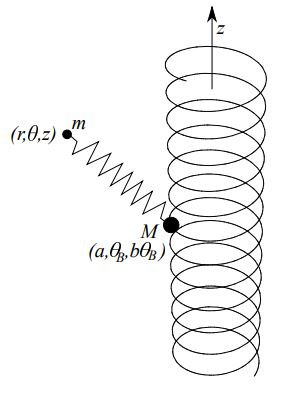
\includegraphics[scale=0.5]{2016TP1Q1.JPG}
\end{figure}
\begin{enumerate}[label=(\alph*)]
\item Show that, up to irrelevant constants and ignoring gravity, the Lagrangian for the system is:\\ 

\hfill\textbf{[6]}
$$\mathcal{L}=\frac{1}{2}m\bigg((\dot{r}^2+r^2\dot{\theta}^2+z^2)+\frac{M}{m}(a^2\dot{\theta}_B^2+b^2\dot{\theta}_B^2)\bigg)-\frac{1}{2}k(r^2-2ar\cos(\theta-\theta_B)+(z-b\theta_B)^2)$$
\item Find the corresponding equations of motion for the particle and the bead.\hfill\textbf{[5]}
\item The system has a helical symmetry. Find the corresponding conserved quantity.\hfill\textbf{[8]}
\item The particle is released from rest at $(r_0, \theta_0, z_0)$. A time $T$ later it is at $(r_0, \theta_0, z_0 + \Delta z)$. If the mass of the bead is negligible, show that
$$\Delta z=-\frac{2A}{b}$$
where $A$ is a geometric property of the particle’s trajectory, and give the geometric interpretation of $A$.\hfill\textbf{[6]}
\end{enumerate}
\end{qns}
\begin{ans}\leavevmode
\begin{enumerate}[label=(\alph*)]
\item The kinetic energies of the free particle and the bead are respectively $\frac{1}{2}m(\dot{r}^2+r^2\dot{\theta}^2+\dot{z}^2)$ and $\frac{1}{2}M(a^2\dot{\theta}_B^2+b^2\dot{\theta}_B^2)$. The potential energy of the string is
$$V=\frac{1}{2}k((r\cos\theta-a\cos\theta_B)^2+(r\sin\theta-a\sin\theta_B)^2+(z-b\theta_B)^2)=\frac{1}{2}k(r^2+a^2-2ar\cos(\theta-\theta_B)+(z-b\theta_B)^2)$$
where $\cos(\theta-\theta_B)=\cos\theta\cos\theta_B+\sin\theta\sin\theta_B$. The Lagrangian is then
$$\mathcal{L}=\frac{1}{2}m(\dot{r}^2+r^2\dot{\theta}^2+z^2)+\frac{1}{2}M(a^2\dot{\theta}_B^2+b^2\dot{\theta}_B^2)-\frac{1}{2}k(r^2+a^2-2ar\cos(\theta-\theta_B)+(z-b\theta_B)^2)$$
but $\mathcal{L}$ is unique up to a constant, so we may discard $\frac{1}{2}ka^2=\text{const}$.
\item Using the Euler-Lagrange equations:
$$\frac{\partial\mathcal{L}}{\partial\theta}=-kar\sin(\theta-\theta_B),\quad\frac{d}{dt}\frac{\partial\mathcal{L}}{\partial\dot{\theta}}=\frac{d}{dt}(mr^2\dot{\theta})=2m\dot{r}r\dot{\theta}+mr^2\ddot{\theta}$$
$$\frac{\partial\mathcal{L}}{\partial r}=mr\dot{\theta}^2-kr+ak\cos(\theta-\theta_B),\quad\frac{d}{dt}\frac{\partial\mathcal{L}}{\partial\dot{r}}=m\ddot{r}$$
$$\frac{\partial\mathcal{L}}{\partial\theta_B}=kar\sin(\theta-\theta_B)+k(z-b\theta_B)b,\quad\frac{d}{dt}\frac{\partial\mathcal{L}}{\partial\dot{\theta}_B}=\ddot{\theta}_BM(a^2+b^2)$$
$$\frac{\partial\mathcal{L}}{\partial z}=-k(z-b\theta_B),\quad\frac{d}{dt}\frac{\partial\mathcal{L}}{\partial\dot{z}}=m\ddot{z}$$
which gives
$$ka\sin(\theta-\theta_B)+mr\ddot{\theta}+2m\dot{r}\dot{\theta}=0,\quad m\ddot{r}-mr\dot{\theta}^2+kr-ka\cos(\theta-\theta_B)$$ 
$$\ddot{\theta}_BM(a^2+b^2)-bk(z-b\theta_B)-kar\sin(\theta-\theta_B)=0,\quad m\ddot{z}+k(z-b\theta_B)=0$$
\item The potential $V(r,\theta-\theta_B,z-\theta_Bb)$ has helical symmetry, i.e. invariant under $\theta\rightarrow\theta+c$, $\theta_B\rightarrow\theta_B+c$ and $z\rightarrow z+cb$. In another words, invariant under simultaneous rotation and elevation of both masses. It follows that the Lagrangian must have the form $\mathcal{L}(\dot{r},\dot{\theta},\dot{z},\dot{\theta}_B,r,\theta-\theta_B,z-b\theta_B)$, and so from Noether's theorem, the conserved quantity is
$$\frac{\partial\mathcal{L}}{\partial\dot{\theta}}\frac{\partial(\theta+c)}{\partial c}\bigg|_{c=0}+\frac{\partial\mathcal{L}}{\partial\dot{\theta}_B}\frac{\partial(\theta_B+c)}{\partial c}\bigg|_{c=0}+\frac{\partial\mathcal{L}}{\partial\dot{z}}\frac{\partial(z+cb)}{\partial c}\bigg|_{c=0}=\frac{\partial\mathcal{L}}{\partial\dot{\theta}_B}+\frac{\partial\mathcal{L}}{\partial\dot{\theta}}+b\frac{\partial\mathcal{L}}{\partial\dot{z}} $$
Denote this as $J$, and check that it is indeed conserved (follows from the equations of motion):
$$J=\frac{\partial\mathcal{L}}{\partial\dot{\theta}_B}+\frac{\partial\mathcal{L}}{\partial\dot{\theta}}+b\frac{\partial\mathcal{L}}{\partial\dot{z}}=M(a^2+b^2)\dot{\theta}_B+mr^2\dot{\theta}+bm\dot{z},\quad\dot{J}=0$$
\item The particle is released from rest, so $J(t=0)=0$ and $J=0$ $\forall t$. Since we have $M=0$ as well,
$$0=J=mr^2\dot{\theta}+bm\dot{z}\implies\int_0^Tr^2\dot{\theta}dt=-b\int_0^T\dot{z}dt=-b\Delta z\implies\Delta z=-\frac{2}{b}\bigg(\frac{1}{2}\int_{t=0}^{t=T}r^2d\theta\bigg)$$
If the particle's trajectory is projected into the horizontal $(r,\theta)$ plane, it forms a closed loop and $A=\frac{1}{2}\int r^2d\theta$ is the area of this loop.
\end{enumerate}
\end{ans}
\newpage
\subsubsection*{2017 Q2}
\begin{qns}
A long solenoid with length $l$ and radius $a$ is centered on the $z$ axis and generates a cylindrically symmetric magnetic field $\mathbf{B}(\rho, z)$, in cylindrical coordinates $(\rho, \theta, z)$. This field is uniform inside the solenoid, $\mathbf{B}=B\mathbf{\hat{z}}$, and negligible outside. A particle with mass $m$ and charge $q$ is fired towards the solenoid from a large distance away with large initial velocity $v\mathbf{\hat{z}}$ and initial radius $\rho_0<a$.
\begin{enumerate}[label=(\alph*)]
\item Show that the relativistic Lagrangian for the particle can be written as
$$\mathcal{L}=-mc^2\sqrt{1-\frac{\dot{z}^2+\dot{\rho}^2+\rho^2\dot{\theta}^2}{c^2}}-V$$
where $V=0$ outside and $-q\rho^2\dot{\theta}B/2$ inside.\hfill\textbf{[5]}
\item The Lagrangian has cylindrical symmetry and does not depend explicitly on time. Find the corresponding conserved quantities, and (given the above initial conditions) find $\dot{\theta}$ for the particle inside the solenoid.\hfill\textbf{[5]}
\item Find the equations of motion for $z$ and $\rho$ inside and outside the solenoid, and discuss whether $\dot{z}$ is a constant of the motion.\hfill\textbf{[4]}
\item Find the full motion of the particle within the solenoid and draw a
diagram of its path. You may assume without proof that $\rho$ and $\dot{\rho}$ are continuous when the particle enters the solenoid.\\

\hfill\textbf{[7]}
\item Neglecting variations in $\dot{z}$ (which is justified if $v$ is large enough) show that, if a non-interacting beam of particles with equal initial velocity passes through the solenoid, it will be focussed to a point on the $z$-axis a distance
$$f=\frac{v}{\omega}\cot\frac{\omega l}{v}$$
beyond the end of the solenoid, and give an expression for $\omega$. Assume $l < v\pi/(2\omega)$.\hfill\textbf{[4]}
\end{enumerate}
In cylindrical polar coordinates
$$\boldsymbol{\nabla}\times\mathbf{A}=\bigg(\frac{1}{\rho}\frac{\partial A_z}{\partial\theta}-\frac{\partial A_\theta}{\partial A_z}\bigg)\boldsymbol{\hat{\rho}}+\bigg(\frac{\partial A_\rho}{\partial A_z}-\frac{\partial A_z}{\partial\rho}\bigg)\boldsymbol{\hat{\theta}}+\frac{1}{\rho}\bigg(\frac{\partial(\rho A_\theta)}{\partial\rho}-\frac{\partial A_\rho}{\partial\theta}\bigg)\mathbf{\hat{z}}$$
\end{qns}
\begin{ans}\leavevmode
\begin{enumerate}[label=(\alph*)]
\item The general form for the Lagrangian of a relativistic particle moving in an EM field is
$$\mathcal{L}=-\frac{mc^2}{\gamma}-q(\phi-\mathbf{v}\cdot\mathbf{A})$$
The velocity at time $t$ is
$$\mathbf{v}=\dot{z}\mathbf{\hat{z}}+\dot{\rho}\boldsymbol{\hat{\rho}}+\rho\dot{\theta}\boldsymbol{\hat{\theta}}\implies v^2=\dot{z}^2+\dot{\rho}^2+\rho^2\dot{\theta}^2$$
$\mathbf{A}$ in the solenoid, inherits the cylindrical symmetry of the problem since $\mathbf{B}=B\mathbf{\hat{z}}$, so $\mathbf{A}=A(\rho,z)\boldsymbol{\hat{\theta}}$ and from the given formula $\boldsymbol{\nabla}\times\mathbf{A}$ in cylindrical polars, we must have $\rho^{-1}\partial_\rho(\rho A)=B\implies A(\rho,z)=\frac{1}{2}B\rho$. The potential part of the Lagrangian is 0 outside and $-q(-\rho\dot{\theta}\frac{1}{2}B\rho)$ inside. This gives 
$$\mathcal{L}=-mc^2\sqrt{1-\frac{\dot{z}^2+\dot{\rho}^2+\rho^2\dot{\theta}^2}{c^2}}-V$$
where $V=0$ outside and $-q\rho^2\dot{\theta}B/2$ inside.
\item Time invariance means the Hamiltonian is conserved. With the canonical momenta, the Hamiltonian can be found by performing a Legendre transform on the Lagrangian.
$$p_\theta=\frac{\partial\mathcal{L}}{\partial\dot{\theta}}=q\rho A+\gamma m\rho^2\dot{\theta},\quad p_z=\gamma m\dot{z},\quad p_\rho=\gamma m\dot{\rho}$$
$$\implies H=p_z\dot{z}+p_\rho\dot{\rho}+p_\theta\dot{\theta}-\mathcal{L}=\gamma mc^2$$
where $(\dot{z}^2+\dot{\rho}^2+\rho^2\dot{\theta}^2=c^2(1-\gamma^{-2})$. Hence, $\gamma$ (and in turn, the particle speed) is a constant of motion. The cylindrical symmetry suggests that $p_\theta=q\rho A+\gamma m\rho^2\dot{\theta}$ is conserved. At $t=0$, $\dot{\theta}=0=A\implies p_\theta=0$. Hence, inside the solenoid we have
$$\dot{\theta}=-\frac{q\rho A}{\gamma m\rho^2}=-\frac{qB}{2\gamma m}$$
\item Using Euler-Lagrange equations, the $z$-equation of motion is
$$\frac{\partial\mathcal{L}}{\partial z}=0,\quad \frac{d}{dt}\frac{\partial\mathcal{L}}{\partial\dot{z}}=\gamma m\ddot{z}$$
Since $\gamma$ is conserved, $\dot{z}$ is a constant of motion, but only outside and inside the solenoid. This constant differs across regions and changes as the particle enters the solenoids, changing $\dot{\theta}$ as a result. Using the Euler-Lagrange equations again, the $\rho$-equation of motion is
$$\frac{\partial\mathcal{L}}{\partial\rho}=m\gamma\rho\dot{\theta}^2+q\rho\dot{\theta}B,\quad\frac{d}{dt}\frac{\partial\mathcal{L}}{\partial\dot{\rho}}=\gamma m\ddot{\rho}$$
where the $B$ term is zero outside. Now, $\dot{\theta}=-\frac{qB}{2\gamma m}$ inside. Let this be $\dot{\theta}:=-\omega$, then we have
$$\gamma m\ddot{\rho}=m\gamma\rho\omega^2+q\rho B\bigg(-\frac{qB}{2\gamma m}\bigg)=-\frac{q^2B^2\rho}{4m\gamma}$$
We thus have the simple harmonic motion equation for $\rho$, i.e. $\ddot{\rho}=-\rho\omega^2$.
\item Assume $\rho$, $\dot{\rho}$ continuous, we have
$$\theta=-\omega t,\quad\rho=\rho_0\cos\omega t,\quad z=v_i$$
for some $v_i$ and $\rho_0$. Since the particle velocity is a constant of motion, we have $v^2=v_i^2+\rho_0^2\omega^2$. Cast $\rho$ into Cartesians:
$$x=\rho\cos\theta=\rho_0\cos^2\omega t=0.5\rho_0(1+\cos2\omega t),\quad y=\rho\sin\theta=\rho_0\cos\omega t\sin\omega t=0.5\rho_0\sin2\omega t$$
The motion is a helix with the cyclotron frequency $2\omega$ that points along $\mathbf{\hat{z}}$ and has radius $\rho_0/2$ and centre at Cartesian coordinates $(\rho_0/2,0)$.
\item Outside the solenoid, the particle moves in a straight line. After a time $T$, the particle's $\rho$ decreases from a certain value to zero, effectively being focused to a point on the $z$-axis. This value is obtained at time $t'=l/v$, i.e. the time it takes to traverse the entire solenoid. Hence,
$$T=\bigg|\frac{\rho(t=t')}{\dot{\rho}}(t=t')\bigg|=\bigg|\frac{\rho_0\cos(\omega l/v)}{-\rho_0\omega\sin(\omega l/v)}\bigg|=\frac{1}{\omega}\cot\frac{\omega l}{v}$$
This focal length is $f=vT$ as given.
\end{enumerate}
\end{ans}
\newpage
\subsubsection*{2018 Q1}
\begin{qns}
The action for a system consisting of a relativistic charged particle moving in an electromagnetic field is given by
$$S=-\int mc^2 d\tau-\int eA_\mu dx^\mu (t)$$
where $x^\mu=(ct,\mathbf{x})$, $A^\mu=(\phi/c,\mathbf{A})$, and $\tau$ is the proper time.
\begin{enumerate}[label=(\alph*)]
\item Derive the equations of motion in terms of the electric and magnetic fields, given by $\mathbf{E} = −\boldsymbol{\nabla}\phi −\frac{\partial}{\partial t}\mathbf{A}$ and $\boldsymbol{B} = \boldsymbol{\nabla}\times\mathbf{A}$, respectively.\hfill\textbf{[8]}
\item Suppose that $\mathbf{B} = \boldsymbol{0}$, that $\mathbf{E}$ is constant and that at $t = 0$ the particle has velocity $\mathbf{v_0}$. Find the subsequent velocity of the particle.\hfill\textbf{[5]}
\item  Find the limiting velocity of the particle as $t\rightarrow\infty$.\hfill\textbf{[3]}
\item Suppose that instead $\mathbf{E} = \boldsymbol{0}$ (and generically $\mathbf{B}\neq\boldsymbol{0}$). Show that $\gamma$, and hence the total speed, are constant.\hfill\textbf{[4]}
\item Suppose now that $\mathbf{E} = \boldsymbol{0}$ and $\mathbf{B}$ is constant. Show that the time dependence of the perpendicular velocity vector $\mathbf{v_\perp}=\mathbf{v}-\mathbf{B}\frac{(\mathbf{v}\cdot\mathbf{B})}{B^2}$ is periodic and find the period.\hfill\textbf{[5]}
\end{enumerate}
\end{qns}
\begin{ans}\leavevmode
\begin{enumerate}[label=(\alph*)]
\item The proper time is related to time by $dt=\gamma d\tau$, with the 4-vector being $dx^\mu=\frac{dx^\mu}{dt}dt$. The action is then
$$S=-\int\frac{mc^2}{\gamma}dt-\int eA_\mu\frac{dx^\mu}{dt}dt$$
where $A_\mu\frac{dx^\mu}{dt}=-\phi+\mathbf{A}\cdot\mathbf{v}$. By the definition of action, i.e. $S=\int\mathcal{L}dt$, we have the Lagrangian to be
$$\mathcal{L}=-\frac{mc^2}{\gamma}+e\mathbf{A}\cdot\mathbf{v}-e\phi$$
The equations of motion follow from the Euler-Lagrange equations
$$\frac{\partial\mathcal{L}}{\partial\mathbf{v}}=-e\boldsymbol{\nabla}\phi+e\boldsymbol{\nabla}(\mathbf{A}\cdot\mathbf{v}),\quad\frac{d}{dt}\frac{\partial\mathcal{L}}{\partial\mathbf{v}}=\frac{d}{dt}\bigg(\gamma m\frac{\mathbf{v}}{c^2}c^2\bigg)+\frac{d}{dt}e\mathbf{A}=\frac{d}{dt}(\gamma m\mathbf{v})+e\frac{\partial\mathbf{A}}{\partial t}+e(\mathbf{v}\cdot\boldsymbol{\nabla})\mathbf{A}$$
But $\boldsymbol{\nabla}(\mathbf{A}\cdot\mathbf{v})=\mathbf{v}\cdot\boldsymbol{\nabla}\mathbf{A}$ since $\mathbf{v}$ has no spatial dependence. We then finally use
$$\mathbf{v}\times(\boldsymbol{\nabla}\times\mathbf{A})=(\boldsymbol{\nabla}\mathbf{A})\cdot\mathbf{v}-(\mathbf{v}\cdot\boldsymbol{\nabla})\mathbf{A}$$
which can be shown by index notation. Finally, we must have
$$\frac{d}{dt}(\gamma m\mathbf{v})=-e\frac{\partial\mathbf{A}}{\partial t}-e\boldsymbol{\nabla}\phi-e(\mathbf{v}\times(\boldsymbol{\nabla}\times\mathbf{A}))=e(\mathbf{E}+(\mathbf{v}\times\mathbf{B}))$$
\item When $\mathbf{B}=\boldsymbol{0}$, integrate the equation of motion with respect to time, we have
$$\gamma m\mathbf{v}=e\mathbf{E}t+m\gamma_0\mathbf{v_0}$$
Dot it with itself, then divided by $m^2c^2$ and finally use $\gamma^2v^2/c^2=\gamma^2-1$:
$$\gamma^2m^2v^2=|\mathbf{E}et+m\gamma_0\mathbf{v_0}|^2\implies\gamma=\sqrt{1+\frac{|e\mathbf{E}t+m\gamma_0\mathbf{v_0}|^2}{m^2c^2}}$$
By definition of $\gamma$, we then have
$$\mathbf{v}=\frac{e\mathbf{E}t/m+\gamma_0\mathbf{v_0}}{\sqrt{1+\frac{|e\mathbf{E}t+m\gamma_0\mathbf{v_0}|^2}{m^2c^2}}}$$
\item For large times, $\mathbf{v}$ will be parallel (or anti-parallel) to $\mathbf{E}$ as long as $|\mathbf{v}|<c$, and this is independent of $\mathbf{v_0}$, i.e.
$$\lim_{t\rightarrow\infty}\mathbf{v}=\frac{e\mathbf{E}}{|e\mathbf{E}|}c$$
\item Dot the equation of motion with $\mathbf{v}$ to get
$$\mathbf{v}\cdot\frac{d}{dt}(\gamma m\mathbf{v})=e\mathbf{v}\cdot(\mathbf{v}\times\mathbf{B})=0\implies 0=\frac{d\gamma}{dt}mc^2(1-\gamma^{-2})$$
where $|\mathbf{v}|^2=c^2(1-\gamma^{-2})$. Since $\gamma\neq1$, we must have $\frac{d\gamma}{dt}=0$, i.e. $\gamma$ and in turn $v$ are both constants. 
\item With $\mathbf{E}=\boldsymbol{0}$, the equation of motion is then
$$\frac{d\mathbf{v}}{dt}=\frac{e}{m\gamma}(\mathbf{v}\times\mathbf{B})$$
Take the time derivative and resolve components
$$\frac{d^2\mathbf{v_\perp}}{dt^2}=\frac{e}{m\gamma}(\mathbf{\dot{v}}\times\mathbf{B})=\frac{e^2}{m^2\gamma^2}(\mathbf{v}\times\mathbf{B})\times\mathbf{B}=-\frac{e^2}{m^2\gamma^2}(\mathbf{v}B^2-\mathbf{B}(\mathbf{v}\cdot\mathbf{B}))=-\bigg(\frac{eB}{m\gamma}\bigg)^2\mathbf{v_\perp}$$
This is a SHM equation with frequency $\omega=\frac{eB}{m\gamma}$.
\end{enumerate}
\end{ans}
\newpage
\subsubsection*{2018 Q2}
\begin{qns}
A massless rod of length $\ell$ makes an angle $\theta(t)$ with the vertical, has a point mass $m$ at one end, and is in a constant gravitational field $\mathbf{g} = g\mathbf{\hat{y}}$. The other end of the rod is attached to a horizontal line with a frictionless hinge, and connected to a point along the line by a massless spring of constant $k$ and zero rest length, as illustrated in the figure.
\begin{figure}[H]
    \centering
    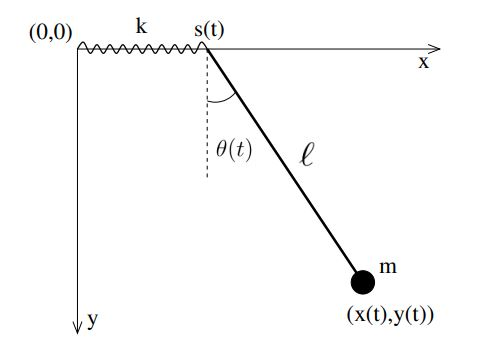
\includegraphics[scale=0.5]{2018TP1Q2.JPG}
\end{figure}
Let us call $s(t)$ the instantaneous horizontal displacement of the hinge from the origin (i.e., the fixed point of the spring).
\begin{enumerate}[label=(\alph*)]
\item Show that the Lagrangian for this system can be written in terms of the dimensionless variables $\eta(t) = s(t)/\ell$ and $\theta(t)$ as
$$\mathcal{L}=\frac{1}{2}(\dot{\eta}^2+2\dot{\eta}\dot{\theta}\cos\theta+\dot{\theta}^2)+\frac{g}{\ell}\cos\theta-\frac{1}{2}\frac{k}{m}\eta^2$$
up to a multiplicative constant.\hfill\textbf{[10]}
\item Find the equations of motion for this system. Then assume that the dynamical variables and their derivatives are small and show that the equations of motion expanded to linear order can be written as
\begin{align}
    \ddot{\theta}+\ddot{\eta}+\omega_0^2\theta&=0\nonumber\\\ddot{\theta}+\ddot{\eta}+\omega_1^2\eta&=0\nonumber
\end{align}
Find the values of the characteristic frequencies $\omega_0$ and $\omega_1$.\hfill\textbf{[8]}
\item Assuming a solution of the form $\theta(t) = \theta_0\sin(\omega t)$, find the corresponding form for $\eta(t)$ and the allowed values of $\omega$. Consider the limit $k\rightarrow\infty$ and discuss briefly whether the result is consistent with your expectation or not.\hfill\textbf{[7]}
\end{enumerate}
\end{qns}
\begin{ans}\leavevmode
\begin{enumerate}[label=(\alph*)]
\item We have the coordinates
$$x=\eta\ell+\ell\sin\theta,~y=\ell\cos\theta\implies\dot{x}=\dot{\eta}\ell+\ell\cos\theta\dot{\theta},~\dot{y}=-\ell\sin\theta\dot{\theta}$$
We then have the kinetic energy to be
$$T=\frac{1}{2}m(\dot{x}^2+\dot{y}^2)=\frac{1}{2}m(\dot{\eta}\ell+\ell\cos\theta\dot{\theta})^2+\ell^2\sin^2\theta\dot{\theta}^2=\frac{1}{2}m\ell^2(\dot{\eta}^2+2\dot{\eta}\cos\theta\dot{\theta}+\dot{\theta}^2)$$
The potential energy is
$$V=-mg\ell\cos\theta+\frac{1}{2}k\eta^2\ell^2$$
The Lagrangian is
$$\mathcal{L}=T-V=\frac{1}{2}m\ell^2(\dot{\eta}^2+2\dot{\eta}\cos\theta\dot{\theta}+\dot{\theta}^2)+mg\ell\cos\theta-\frac{1}{2}k\eta^2\ell^2$$
But since the Lagrangian is unique up to a multiplicative constant, we can drop out the $m\ell^2$ factor.
\item The equation of motion is obtained from the Euler-Lagrange equations
$$\frac{\partial\mathcal{L}}{\partial\theta}=-\dot{\eta}\dot{\theta}\sin\theta-\frac{g}{\ell}\sin\theta,\quad\frac{d}{dt}\frac{\partial\mathcal{L}}{\partial\dot{\theta}}=\ddot{\theta}+\ddot{\eta}\cos\theta-\sin\theta\dot{\eta}\dot{\theta}$$
$$\frac{\partial\mathcal{L}}{\partial\eta}=-\frac{k}{m}\eta,\quad\frac{d}{dt}\frac{\partial\mathcal{L}}{\partial\dot{\eta}}=\ddot{\eta}+\ddot{\theta}\cos\theta-\sin\theta\dot{\theta}^2$$
Using small angle approximation such that $\sin\theta\approx\theta$, $\cos\theta\approx1$ and that $\dot{\eta}, \dot{\theta}$ small so that products of time derivatives are negligible. In that case, we have
$$0=\ddot{\theta}+2\dot{\eta}\dot{\theta}\sin\theta+\frac{g}{\ell}\sin\theta+\ddot{\eta}\cos\theta\approx\ddot{\theta}+\ddot{\eta}+\frac{g}{\ell}\theta$$
$$0=\ddot{\eta}+\frac{k}{m}\eta+\ddot{\theta}\cos\theta-\sin\theta\dot{\theta}^2\approx\ddot{\theta}+\ddot{\eta}+\frac{k}{m}\eta$$
allowing us to read off as $\omega_0^2=g/\ell$ and $\omega_1^2=k/m$.
\item The equations of motion expanded to linear order suggests $\eta=\frac{\omega_0^2}{\omega_1^2}\theta$. Further, given $\theta(t)=\theta_0\sin\omega t$, then
$$\ddot{\theta}=-\omega^2\theta,\quad\ddot{\eta}=-\frac{\omega_0^2\omega^2}{\omega_1^2}\theta$$
Plug into the equations of motion will give
$$\omega^2\bigg(1+\frac{\omega_0^2}{\omega_1^2}\bigg)=\omega_0^2\implies\omega^2=\frac{\omega_0^2\omega_1^2}{\omega_0^2+\omega_1^2}$$
As $k\rightarrow\infty$, $\omega_1^2\rightarrow\infty$, $\eta\rightarrow 0$ and hence $\omega^2\approx\omega_0^2=g/l$. The top hinge is fixed with infinite spring stiffness, within the approximation regime of small oscillations.
\end{enumerate}
\end{ans}
\newpage
\subsubsection*{2019 Q1}
\begin{qns}\leavevmode
\begin{enumerate}[label=(\alph*)]
\item Describe what is meant by a holonomic constraint in Lagrangian classical mechanics and give an example of a system with a holonomic constraint.\hfill\textbf{[4]}
\item A uniform cylinder of mass $m$ and radius $r$ rolls without slipping inside a larger cylinder of radius $R$. The angles $\theta$ and $\phi$ are defined as in the Figure, where the black dots coincide when the rolling cylinder is at its lowest point.
\begin{figure}[H]
    \centering
    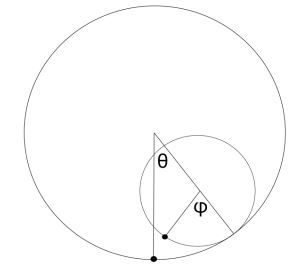
\includegraphics[scale=0.7]{2019TP1Q2.JPG}
\end{figure}
By resolving the motion into the motion of the centre of mass and motion about the centre of mass, show that the kinetic energy may be written as\hfill\textbf{[5]}
$$\frac{m}{2}(R-r)^2\dot{\theta}^2+\frac{m}{4}r^2(\dot{\phi}-\dot{\theta})^2$$
\item Show that the no slip condition yields a holonomic constraint.\hfill \textbf{[3]}
\item By writing down the Lagrangian, show that the system can exhibit small oscillations and find the corresponding oscillation frequency.\hfill\textbf{[6]}
\item Discuss whether or not there is a frictional force present and whether or not the energy of the system is conserved.\hfill\textbf{[3]}
\item Discuss whether or not angular momentum is conserved.\hfill\textbf{[2]}
\item Discuss whether or not the system is holonomic for all possible motions.\hfill\textbf{[2]}
\end{enumerate}
\end{qns}
\begin{ans}\leavevmode
\begin{enumerate}[label=(\alph*)]
\item Holonomic constraints can be expressed in terms of generalized coordinates and time. The scenario (no slip condition) in the question is one such example, if the oscillations are small enough.
\item The motion of the Centre of Mass is purely rotational, in a circle of radius $R-r$ with angular velocity $\dot{\theta}$. Rotation of cylinder about its CoM in the rest frame is with angular velocity $\dot{\phi}-\dot{\theta}$. The kinetic energy is the sum of the translational kinetic energy and that due to self-rotation, i.e.
$$T=\frac{1}{2}m(R-r)^2\dot{\theta}^2+\frac{1}{2}\frac{1}{2}mr^2(\dot{\phi}-\dot{\theta})^2$$
\item The no slip condition gives $r\phi=R\theta$ and is a holonomic constraint.
\item The potential energy is $V=-mg(R-r)\cos\theta$, and so the Lagrangian is
\begin{align}
\mathcal{L}=T-V&=\frac{1}{2}m(R-r)^2\dot{\theta}^2+\frac{1}{4}mr^2(\dot{\phi}-\dot{\theta})^2+mg(R-r)\cos\theta\nonumber\\&=\frac{1}{2}m(R-r)^2\dot{\theta}^2+\frac{1}{4}m(R-r)^2\dot{\theta}^2+mg(R-r)\cos\theta\nonumber\\&=\frac{3}{4}m(R-r)^2\dot{\theta}^2+mg(R-r)\cos\theta\nonumber
\end{align}
where the no-slip condition gives $(\dot{\phi}-\dot{\theta})=\frac{R-r}{r}\dot{\theta}$. The equations of motion is obtained from the Euler-Lagrange equations
$$\frac{\partial\mathcal{L}}{\partial\theta}=-mg(R-r)\sin\theta,\quad\frac{d}{dt}\frac{\partial\mathcal{L}}{\partial\dot{\theta}}=\frac{3}{2}m(R-r)^2\ddot{\theta}$$
which gives $(R-r)\ddot{\theta}=\frac{2}{3}g\theta$, which is a SHM equation with oscillation frequency $\omega^2=\frac{2g}{3(R-r)}$.
\item There must be friction present to ensure the cylinder rolls without slipping. However, this force does no work because the motion is always normal to it. Hence, the total energy is conserved, consistent with the fact that $\mathcal{L}$ is explicitly independent of time.
\item The angular momentum is $p_\theta=\frac{\partial\mathcal{L}}{\partial\dot{\theta}}$. Its rate of change is
$$\frac{d}{dt}p_\theta=\frac{d}{dt}\frac{\partial\mathcal{L}}{\partial\dot{\theta}}=\frac{\partial\mathcal{L}}{\partial\theta}=-mg(R-r)\sin\theta\neq 0$$
i.e. the angular momentum is not conserved due to gravity.
\item For large motions, the small cylinder can lose contact with the larger cylinder. The system cannot be expressed in generalized coordinates alone, so the system is holonomic.
\end{enumerate}
\end{ans}
\subsubsection*{2020 Q1}
\begin{qns}
Two identical beads of mass $m$ are each attached to a pivot point P by a light spring of constant $\kappa$ and unstretched length $\ell= 0$, in the presence of a gravitational acceleration $g$. They are further connected to one another by a spring of constant $\kappa'$ and unstretched length $\ell'>0$. The centres of the two beads are confined to move within a vertical plane through P, as sketched below.
\begin{figure}[H]
    \centering
    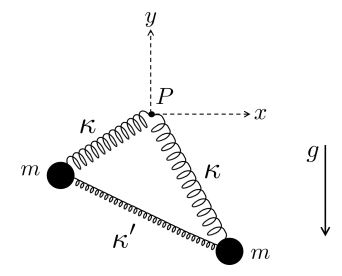
\includegraphics[scale=0.65]{2020TP1Q1.JPG}
\end{figure}
\begin{enumerate}[label=(\alph*)]
\item Show that the Lagrangian of the system can be written as
\begin{align}
\mathcal{L}&=m(\dot{X}^2+\dot{Y}^2)-2mg(Y-\alpha)-\kappa[X^2+(Y-\alpha)^2]\nonumber\\&+m(\dot{x}^2+\dot{y}^2)-\kappa(x^2+y^2)-2\kappa'\bigg(\sqrt{x^2+y^2}-\frac{\ell'}{2}\bigg)^2\nonumber
\end{align}
where $X = (x_1 + x_2)/2$, $Y = (y_1 + y_2)/2 + \alpha$, $x = (x_1 − x_2)/2$, $y = (y_1 − y_2)/2$. Here, $(x_1, y_1)$ and $(x_2, y_2)$ denote the coordinates of the centres of the two beads in the Cartesian reference frame given by the dashed axes in the figure, and $\alpha$ is a generic constant. Find the Euler-Lagrange equations of motion of the system.\hfill\textbf{[7]}
\item Find the equilibrium positions of the beads and show that, for an appropriate choice of $\alpha$, they satisfy\hfill\textbf{[6]}
$$X=Y=0,\quad x^2+y^2=\bigg(\frac{\kappa'\ell'}{\kappa+2\kappa'}\bigg)^2$$
\item For the value of $\alpha$ chosen in (b), find the normal modes and the corresponding frequencies of small oscillations about the equilibrium positions.\hfill\textbf{[8]}
\item Discuss the continuous symmetries of the Lagrangian and find the corresponding conserved quantities.\hfill\textbf{[4]}
\end{enumerate}
\end{qns}
\begin{ans}\leavevmode
\begin{enumerate}[label=(\alph*)]
\item The kinetic energy is
\begin{align}
    T&=\frac{1}{2}m(\dot{x}_1^2+\dot{y}_1^2+\dot{x}_2^2+\dot{y}_2^2)\nonumber\\&=m(0.25(\dot{x}_1+\dot{x}_2)^2+0.25(\dot{y}_1+\dot{y}_2)^2+0.25(\dot{x}_1-\dot{x}_2)^2+0.25(\dot{y}_1-\dot{y}_2)^2)\nonumber\\&=m(\dot{X}^2+\dot{x}^2+\dot{Y}^2+\dot{y}^2)\nonumber
\end{align}
The potential energy is
\begin{align}
    V&=mg(y_1+y_2)+\frac{1}{2}\kappa(x_1^2+y_1^2)+\frac{1}{2}\kappa(x_2^2+y_2^2)+\frac{1}{2}\kappa'(\sqrt{(x_1-x_2)^2+(y_1-y_2)^2}-\ell')^2\nonumber\\&=2mg(Y-\alpha)+\kappa(0.5x_1^2+0.5x_2^2+0.5y_1^2+0.5y_2^2)+0.5\kappa'(2\sqrt{(0.5(x_1-x_2))^2+(0.5(y_1-y_2))^2}-\ell')^2\nonumber\\&=2mg(Y-\alpha)+\kappa(X^2+(Y-\alpha)^2+x^2+y^2)+2\kappa'(\sqrt{x^2+y^2}-0.5\ell')^2\nonumber
\end{align}
The Lagrangian is then
$$\mathcal{L}=T-V=m(\dot{X}^2+\dot{Y}^2)-2mg(Y-\alpha)-\kappa[X^2+(Y-\alpha)^2]+m(\dot{x}^2+\dot{y}^2)-2\kappa'\bigg(\sqrt{x^2+y^2}-\frac{\ell'}{2}\bigg)^2$$
The equation of motion is satisfied by the Euler-Lagrange equations
$$\frac{\partial\mathcal{L}}{\partial X}=-2\kappa X,\quad\frac{d}{dt}\frac{\partial\mathcal{L}}{\partial\dot{X}}=\frac{d}{dt}(2m\dot{X})=2m\ddot{X}\implies m\ddot{X}=-\kappa X$$
$$\frac{\partial\mathcal{L}}{\partial Y}=-2\kappa(Y-\alpha)-2mg,\quad\frac{d}{dt}\frac{\partial\mathcal{L}}{\partial\dot{Y}}=\frac{d}{dt}(2m\dot{Y})=2m\ddot{Y}\implies m\ddot{Y}=-\kappa Y-mg+\kappa\alpha$$
$$\frac{\partial\mathcal{L}}{\partial x}=-2\kappa x-2\kappa'2(\sqrt{x^2+y^2}-0.5\ell')\frac{x}{\sqrt{x^2+y^2}}=-2\kappa x-\frac{4\kappa'x(\sqrt{x^2+y^2}-0.5\ell')}{\sqrt{x^2+y^2}},\quad\frac{d}{dt}\frac{\partial\mathcal{L}}{\partial\dot{x}}=2m\ddot{x}$$
$$\implies m\ddot{x}=-\kappa x-2\kappa'(\sqrt{x^2+y^2}-0.5\ell')\frac{x}{\sqrt{x^2+y^2}}$$
$$\frac{\partial\mathcal{L}}{\partial y}=-2\kappa y-2\kappa'2(\sqrt{x^2+y^2}-0.5\ell')\frac{y}{\sqrt{x^2+y^2}}=-2\kappa y-\frac{4\kappa'y(\sqrt{x^2+y^2}-0.5\ell')}{\sqrt{x^2+y^2}},\quad\frac{d}{dt}\frac{\partial\mathcal{L}}{\partial\dot{y}}=2m\ddot{y}$$
$$\implies m\ddot{y}=-\kappa y-2\kappa'(\sqrt{x^2+y^2}-0.5\ell')\frac{y}{\sqrt{x^2+y^2}}$$
\item In equilibrium, $\ddot{X}=0=\ddot{Y}$, which gives us $X=0$, $Y=-(mg/k)+\alpha$. In order for $Y-0$, we must choose $\alpha=mg/k$. Also, $\ddot{x}=0=\ddot{y}$ which gives either $x=0=y$ which is not a valid solution since we needed $x^2+y^2>0$ to derive our equations of motion (and that this solution is physically not possible since in this configuration, there are net forces and the system is not in equilibrium) or the relative coordinate of one bead with respect to the other forms a circle of radius $\frac{\kappa'\ell'}{\kappa+2\kappa'}$, i.e.
$$\sqrt{x^2+y^2}=\frac{\kappa'\ell'}{\kappa+2\kappa'}$$
\item With $\alpha=mg/\kappa$, we have that $X$ and $Y$ to be SHM equations with frequency $\Omega=\sqrt{\kappa/m}$ around the equilibrium position (0,0). The degenerate frequencies in both directions, due to the rotational symmetry in the $(X,Y)$-plane. We expand about the equilibrium $(x_0,y_0)$, i.e. $x=x_0+\delta x$ and $y=y_0+\delta y$. 
$$x^2+y^2=(x_0+\delta x)^2+(y_0+\delta y)^2=x_0^2+y_0^2+2x_0\delta x+2y_0\delta y$$
$$\frac{1}{\sqrt{x^2+y^2}}=\frac{1}{\sqrt{x_0^2+y_0^2}}\bigg(1+\frac{2x_0\delta x+2y_0\delta y}{x_0^2+y_0^2}\bigg)^{-1/2}\approx\frac{1}{\sqrt{x_0^2+y_0^2}}-\frac{x_0\delta x+y_0\delta y}{\sqrt{x_0^2+y_0^2}}$$
Hence, expand the equations of motion:
\begin{align}
m\ddot{x}&=-(\kappa+2\kappa')x+\frac{x}{\sqrt{x^2+y^2}}\kappa'\ell'\nonumber\\\sqrt{x_0^2+y_0^2}=\frac{\kappa'\ell'}{\kappa+2\kappa'}\implies m\delta\ddot{x}&=\frac{x_0+\delta x}{\sqrt{x_0^2+y_0^2}}(\kappa'\ell'-\kappa'\ell'-\frac{\kappa+2\kappa'}{\sqrt{x_0^2+y_0^2}}(x_0\delta x+y_0\delta y))\nonumber\\&=\frac{-(\kappa+2\kappa')^3}{\kappa'^2\ell'^2}x_0(x_0\delta x+y_0\delta y)\nonumber
\end{align}
Similarly, $m\delta\ddot{y}=-\frac{(\kappa+2\kappa')^3}{\kappa'^2\ell'^2}y_0(x_0\delta x+y_0\delta y)$. We can then cast them into a matrix form
$$\begin{pmatrix}\delta\ddot{x}\\\delta\ddot{y}\\\end{pmatrix}=-\frac{(\kappa+2\kappa')^3}{\kappa'^2\ell'^2m}\begin{pmatrix}x_0^2&x_0y_0\\x_0y_0&y_0^2\\\end{pmatrix}\begin{pmatrix}\delta x\\\delta y\\\end{pmatrix}$$
Set determinant as zero, we then have the eigenvalues to be
$$0=\det\begin{pmatrix}x_0^2-\lambda&x_0y_0\\x_0y_0&y_0^2-\lambda\\\end{pmatrix}=\lambda^2-\lambda(x_0^2+y_0^2)\implies\lambda=0,~x_0^2+y_0^2$$
Scale the eigenvalues by the factor $\frac{(\kappa+2\kappa')^3}{\kappa'^2\ell'^2m}$:
$$\omega=0,\quad\omega^2=(x_0^2+y_0^2)\frac{(\kappa+2\kappa')^3}{(\kappa'\ell')^2m}=\frac{\kappa'^2\ell'^2}{(\kappa+2\kappa')^2}\frac{(\kappa+2\kappa')^3}{(\kappa'\ell')^2m}=\frac{\kappa+2\kappa'}{m}$$
where their eigenvectors (normal modes) respectively are
$$\begin{pmatrix}\delta x\\\delta y\\\end{pmatrix}=\begin{pmatrix}y_0\\-x_0\\\end{pmatrix},\quad\begin{pmatrix}\delta x\\\delta y\\\end{pmatrix}=\begin{pmatrix}x_0\\y_0\\\end{pmatrix}$$
where the former (zero-frequency mode) is due to rotational symmetry in the $(x,y)$ plane.
\item We see that the Lagrangian $\mathcal{L}$ does not depend explicitly on time and hence the Hamiltonian is conserved. Only the action and not the Lagrangian is invariant under time translations. We define $\boldsymbol{r}=(x,y)^T$ and $\mathbf{R}=(X,Y)^T$. Then, 
$$\mathcal{L}=m(\dot{r}^2+\dot{R}^2)+\frac{m^2g^2}{\kappa}-\kappa(r^2+R^2)-2\kappa'(r-0.5\ell')^2$$
which is clearly invariant under independent rotations, i.e. $\mathbf{r}\rightarrow M\mathbf{r}$ and $\mathbf{R}\rightarrow M'\mathbf{R}$. We cast into plane polar coordinates $\mathbf{r}=(r,\theta)^T$ and $\mathbf{R}=(R,\phi)^T$:
$$\mathcal{L}=m(\dot{r}^2+r^2\dot{\theta}^2+\dot{R}^2+R^2\phi^2)+\frac{m^2g^2}{\kappa}-\kappa(r^2+R^2)-2\kappa'(r-0.5\ell')^2$$
which is independent of $\theta$ and $\phi$. Hence, their canonical momenta are conserved.
$$\frac{dp_\theta}{dt}=\frac{d}{dt}\frac{\partial\mathcal{L}}{\partial\dot{\theta}}=\frac{\partial\mathcal{L}}{\partial\theta}=0$$
which implies $p_\theta=\frac{\partial\mathcal{L}}{\partial\dot{\theta}}=2mr^2\dot{\theta}$ is conserved. Similarly, $p_\phi=2mR^2\dot{\phi}$ is conserved. But, in the original coordinates, we have
$$p_\theta=m(x\dot{y}-y\dot{x})=m\frac{1}{4}(x_1\dot{y}_1-x_1\dot{y}_2-x_2\dot{y}_1+x_2\dot{y}_1-y_1\dot{x}_1+y_1\dot{x}_2+y_2\dot{x}_1-y_2\dot{x}_2)$$
$$p_\phi=m(X\dot{Y}-Y\dot{X})=m\frac{1}{4}(x_1\dot{y}_1+x_1\dot{y}_2+x_2\dot{y}_1+x_2\dot{y}_2-y_1\dot{x}-1-y_2\dot{x}_1-y_1\dot{x}_2-y_2\dot{x}_2)-\frac{1}{2}(\dot{x}_1+\dot{x}_2)\frac{mg}{k}$$
The sum of the two conserved quantities is proportional to $J^z_{tot}-\frac{mg}{\kappa}p_{tot}^x$, i.e. the $z$-component of the total angular momentum $J_{\text{tot}}^z=m\sum_ix_i\dot{y}_i-\dot{x}_iy_i$, and the $x$-component of the total linear momentum of the system $p_{\text{tot}}^x=m(\dot{x}_1+\dot{x}_2)$.
\end{enumerate}
\end{ans}
\newpage
\section{Classical Field Theory}
\subsection{Classical fields}
\subsubsection{Relativistic scalar fields}
\begin{defi}[Scalar field]
We consider scalar fields $\phi(x):=\phi(t,\mathbf{x})$ where $x$ is a mere label in field theory and no longer a dynamical variable. 
$$\phi:~\mathbb{R}^{3,1}\rightarrow\mathbb{R}$$
where the field takes in a spacetime coordinate and outputs a scalar.
\end{defi}
We want to construct field theories in which space and time are placed on an equal footing and the theory is invariant under Lorentz transform.
\begin{defi}[Lorentz transform fields]
The Lorentz transformations have a representation on the fields. Under the Lorentz transform $x\rightarrow\Lambda x$, the scalar field transforms (actively) as
$$\phi(x)\rightarrow\phi'(x)=\phi(\Lambda^{-1}x)$$
For a Lorentz invariant theory, if $\phi(x)$ solves the equations of motion then $\phi(\Lambda^{-1}x)$ also solves the equations of motion. 
\end{defi}
\begin{remarks}
The inverse $\Lambda^{-1}$ appears in the argument because we are dealing with an active transformation in which the field is truly shifted, i.e. the new field at the new coordinate equals the old field at the old coordinate. If we were instead dealing with a passive transformation in which we relabel our choice of coordinates, we would have instead $\phi(x)\rightarrow\phi'(x)=\phi(\Lambda x)$. Note that for active transformation,
$$(\Lambda^{-1}x)^\mu=\tensor*{(\Lambda^{-1})}{*_{}^{\mu}_{\nu}}x^\nu$$
where $\tensor*{(\Lambda^{-1})}{*_{}^{\mu}_{\nu}}\tensor*{(\Lambda)}{*_{}^{\nu}_{\rho}}=\tensor*{\delta}{*_{}^{\mu}_{\rho}}$.
\end{remarks}
\begin{defi}[Spacetime Derivative]
We define the spacetime derivative to be
$$\partial_\mu\phi(x):=\frac{\partial\phi(x)}{\partial x^\mu}$$
which transforms as
$$\partial_\mu\rightarrow\frac{\partial x^\nu}{\partial x'^\mu}\partial_\nu\implies\partial_\mu\phi(x)\rightarrow\tensor*{(\Lambda^{-1})}{*_{}^{\nu}_{\mu}}\partial_\nu\phi(\Lambda^{-1}x)$$
and to raise the index, $\partial^\mu\phi(x)=\eta^{\mu\nu}\partial_\nu\phi(x)$. One can then show that $\partial^\mu\phi(x)$ transforms as a 4-vector field
$$\partial^\mu\phi(x)\rightarrow\tensor*{\Lambda}{*_{}^{\mu}_{\nu}}\partial^\nu\phi(\Lambda^{-1}x)$$
\end{defi}
\begin{prop}
The following transforms like a scalar field:
$$\partial_\mu\phi(x)\partial^\mu\phi(x)=\eta^{\mu\nu}\partial_\mu\phi(x)\partial_\nu\phi(x)$$
\end{prop}
The Lagrangian for a scalar field $\phi(x)=\phi(\mathbf{x},t)$ is demanded to satisfy the following:
\begin{itemize}
    \item the action is Lorentz invariant (not the same as Lagrangian being Lorentz invariant)
    \item locality
    \item at most two time derivatives
\end{itemize}
The Lagrangian will then be a scalar function of $\phi$ and its spacetime derivatives $\partial_\mu$ to ensure later Lorentz invariant. To ensure locality, we write the Lagrangian as an integral over position.
\begin{defi}[Lagrangian density]
The Lagrangian density defined at a position $x$, $\mathcal{L}(\phi(x),\partial_\mu\phi(x))$, satisfies
$$L(t)=L[\phi,\partial_\mu\phi]=\int\mathcal{L}(\phi(x),\partial_\mu\phi(x))d^3x$$
\end{defi}
\begin{notation}
By abuse of terminology, we will now call $\mathcal{L}$ the Lagrangian.
\end{notation}
\begin{defi}[Action]
The corresponding action for the Lagrangian density is
$$S_{t_i,t_f}[\phi,\partial_\mu\phi]=\int_{t_i}^{t_f}\int\mathcal{L}d^3dt$$
For most purposes, we work with an infinite time interval, $t_i\rightarrow-\infty$ and $t_f\rightarrow+\infty$. The action is then
$$S[\phi,\partial_\mu\phi]=\int_{\mathbb{R}^{3,1}}\mathcal{L}[\phi(x),\partial_\mu\phi(x)]d^4x$$
\end{defi}
\begin{prop}
The action associated with the Lagrangian $\mathcal{L}(x)=\mathcal{L}[\phi,\partial_\mu\phi]=\mathcal{L}(\phi(x),\partial_\mu\phi(x))$ is indeed Lorentz invariant.
\end{prop}
\begin{proof}
Under Lorentz transformation, i.e. $x^\mu\rightarrow x'^\mu=\tensor*{\Lambda}{*_{}^{\mu}_{\nu}}x^\nu$, we have
$$\mathcal{L}(x)\rightarrow\mathcal{L}(\Lambda^{-1}\cdot x)\implies S=\int\mathcal{L}(x)d^4x\rightarrow S'=\int\mathcal{L}(\Lambda^{-1}\cdot x)d^4x$$
where we next do a change of variables $y^\mu=\tensor*{(\Lambda^{-1})}{*_{}^{\mu}_{\nu}}x^\nu$ and since $\det\Lambda=1$, $S'=\int\mathcal{L}(y)d^4y=S$.
\end{proof}
\begin{remarks}
This is actually a consequence of the Lagrangian being a scalar field. Essentially, there are two requirements for any Lagrangian: it must be a Lorentz scalar and contains less than 3 time derivatives. The most general Lagrangian that fulfills the requirement is
$$\mathcal{L}=\frac{1}{2}F(\phi)\partial_\mu\phi\partial^\mu\phi-V(\phi)$$
$\phi\partial_\mu\partial^\mu\phi$ gives a total derivative, which simplifies to a surface term contribution to the action, which is not important due to our boundary condition (see later). For simplicity, consider only $F(\phi)=1$.
\end{remarks}
Before we proceed, we remind everyone the method of Lagrange multipliers:
\begin{prop}[Method of Lagrange Multipliers]
Consider multiple constraints, say $k$ of them. We want to extremize $f:\mathbb{R}^n\rightarrow\mathbb{R}$, subject to $k$ of these constraints $g_\alpha(\mathbf{x})=0$, where $\alpha=1,\dots,k$. We define the function $h(\mathbf{x}_1,\dots,\mathbf{x}_n,\lambda_1,\dots,\lambda_k)$ which is a multi-variate function of $n+k$ variables. The method of Lagrange multipliers will give us the extrema if we solve for
$$\frac{\partial h(\mathbf{x},\boldsymbol{\lambda})}{\partial x_i}=0,\quad\frac{\partial h(\mathbf{x},\boldsymbol{\lambda})}{\partial\lambda_\alpha}=0$$
where $\mathbf{x}\in\mathbb{R}^n$, $\boldsymbol{\lambda}\in\mathbb{R}^k$, $\alpha=1,\dots,k$ and $i=1,\dots,n$.  
\end{prop}
\begin{prop}[Euler-Lagrange equations]
$$\frac{\partial\mathcal{L}}{\partial\phi}=\partial_\mu\bigg(\frac{\partial\mathcal{L}}{\partial(\partial_\mu\phi)}\bigg)$$
\end{prop}
\begin{proof}
Consider principle of least action again. Vary the field configuration $\phi(x)\rightarrow\phi(x)+\delta\phi(x)$, subject to the boundary conditions
$$\delta\phi(x)=\delta\phi(t,\mathbf{x})\rightarrow 0,\quad\text{for}~|\mathbf{x}|\rightarrow\infty,~\text{or}~t\rightarrow\pm\infty$$
The variation of action will then be
$$\delta S=\int\bigg[\frac{\partial\mathcal{L}}{\partial\phi}\delta\phi+\frac{\partial\mathcal{L}}{\partial(\partial_\mu\phi)}\delta(\partial_\mu\phi)\bigg]d^4x=\int\bigg[\frac{\partial\mathcal{L}}{\partial\phi}-\partial_\mu\bigg(\frac{\partial\mathcal{L}}{\partial(\partial_\mu\phi)}\bigg)\bigg]\delta\phi d^4x+\int\partial_\mu\bigg(\frac{\partial\mathcal{L}}{\partial(\partial_\mu\phi)}\delta\phi\bigg)d^4x$$
where we performed intergration by parts and invoked the boundary conditions. The second term, by Stokes' theorem, gives a pure surface term
$$\int_{\partial\mathbb{R}^{3,1}}\frac{\partial\mathcal{L}}{\partial(\partial_\mu\phi)}dS_\mu$$
which again vanishes due to our boundary conditions. Hence, for vanishing action, $\delta S=0$,
$$\int\bigg[\frac{\partial\mathcal{L}}{\partial\phi}-\partial_\mu\bigg(\frac{\partial\mathcal{L}}{\partial(\partial_\mu\phi)}\bigg)\bigg]\delta\phi=0\quad\forall\delta\phi$$
which gives our Euler-Lagrange equations.
\end{proof}
\begin{cor}
The `equation of motion' for the most generic Lagrangian $\mathcal{L}=\frac{1}{2}(\partial_\mu\phi)(\partial^\mu\phi)-V(\phi)$ is
$$\partial_\mu\partial^\mu\phi+V'(\phi)=0$$
\end{cor}
\begin{proof}
We have $\frac{\partial\mathcal{L}}{\partial\phi}=-V'(\phi)$ and $\frac{\partial\mathcal{L}}{\partial(\partial_\mu\phi)}=\partial^\mu\phi$, finally invoke Euler-Lagrange equation.
\end{proof}
\begin{eg}[Klein-Gordon equation]
Consider $V(\phi)=\frac{1}{2}m^2\phi^2$, then the `equation of motion' is called the Klein-Gordon equation
$$\partial_\mu\partial^\mu\phi+m^2\phi=0$$
where $\partial_\mu\partial^\mu=\frac{\partial^2}{\partial t^2}-\sum_i\frac{\partial^2}{\partial x_i^2}=\Box$ is the spacetime Laplacian. The Klein-Gordon equation is a linear PDE with wavelike solutions $\phi\sim e^{i x\cdot p}=e^{i\omega t-i\mathbf{k}\cdot\mathbf{x}}$ with dispersive relation $\omega_{\mathbf{k}}=\sqrt{|\mathbf{k}|^2+m^2}$. The general solution is a superposition of localized wavepackets.
\end{eg}
\begin{defi}[Conjugate momentum]
Define momentum $\pi(\mathbf{x},t)$ conjugate to $\phi(\mathbf{x},t)$ as
$$\pi(\mathbf{x},t)=\frac{\partial\mathcal{L}(\mathbf{x},t)}{\partial\dot{\phi}(\mathbf{x},t)}$$
We may also suppress index $t$ and work at a fixed time $\phi(x):=\phi(\mathbf{x},t)$ and $\pi(x):=\pi(\mathbf{x},t)$.
\end{defi}
\begin{defi}[Hamiltonian density]
Perform Legendre transform to the Lagrangian density, we can obtain the Hamiltonian density
$$H:=H(\phi(\mathbf{x},t),\pi(\mathbf{x},t))=\pi(\mathbf{x},t)\dot{\phi}(\mathbf{x},t)-\mathcal{L}(\mathbf{x},t)$$
which we will for short, call it the Hamiltonian. 
\end{defi}
\begin{eg}
Consider the Klein-Gordon Lagrangian again
$$\mathcal{L}=\frac{1}{2}(\partial_\mu\phi)(\partial^\mu\phi)-V(\phi)=\frac{1}{2}\dot{\phi}^2-\frac{1}{2}|\boldsymbol{\nabla}\phi|^2-V(\phi)$$
The conjugate momentum is 
$$\pi(\mathbf{x},t)=\frac{\partial\mathcal{L}}{\partial\dot{\phi}}(\mathbf{x},t)=\dot{\phi}(\mathbf{x},t)$$
The Hamiltonian density is
$$H=\pi\dot{q}-\mathcal{L}=\frac{1}{2}\pi^2+\frac{1}{2}|\boldsymbol{\nabla}\phi|^2+V(\phi)=T^{00}$$
which gives the Hamiltonian as the energy, as expected. $T^{\mu\nu}$ is the energy momentum tensor, which we will discuss later.
\end{eg}
\begin{remarks}
The Hamiltonian formalism is not manifestly Lorentz invariant since we picked a preferred time. Despite so, the physics must remain unchanged.
\end{remarks}
\begin{note}[Natural units]
We choose natural units $\hbar=1$, $G=1$ and $c=1$. The dimensional units of the natural constants are $c\sim LT^{-1}$, $\hbar\sim L^2MT^{-1}$ and $G\sim L^3M^{-1}T^{-2}$. All quantities scale with some power of mass and energy. In this case, $L$, $T$, $E$ and $M^{-1}$ have the same dimensions. The action is dimensionless but $S\sim\int\mathcal{L}d^4x$ where $d^4x\sim M^{-4}$. It then follows that $\mathcal{L}$ and $H$ have dimensions $M^4$, hence $\phi$ has dimension $M$. If $X$ has dimensions of (mass) $d$ we will write $[X] = d$, then we write
$$[S]=0,~[d^4x]=-4\implies [\mathcal{L}]=4=[H],\quad [\phi]=1$$
\end{note}
\newpage
\subsubsection{Problems}
\begin{qns}
Natural drainage networks are speculated to minimise $S=\int|Q(x,y)|^\alpha dxdy$ subject to the constraint that $\boldsymbol{\nabla}\cdot\mathbf{Q} = R(x, y)$. Here $\mathbf{Q}$ is a two dimensional vector field for the flow of water across the plane and $R$ is the local rainfall density. Find the Euler-Lagrange equations for $\mathbf{Q}$ in terms of a Lagrange multiplier field for the constraint. (Try $\alpha=2$ as a warm-up case)
\end{qns}
\begin{ans}
By method of Lagrange multipliers, minimizing $S=\int|Q(x,y)|^\alpha dxdy$ subject to the constraint $\boldsymbol{\nabla}\cdot\mathbf{Q}=R(x,y)$ is equivalent to minimizing
$$S'=\int[(Q_x^2+Q_y^2)^{\alpha/2}+\lambda(\boldsymbol{\nabla}\cdot\mathbf{Q}-R)]dxdy$$
without constraint. Let the integrand of $S'$ in the Lagrangian be $\mathcal{L}$. The Euler-Lagrange equation will be
$$\frac{\partial\mathcal{L}}{\partial Q_i}-\frac{\partial}{\partial x}\bigg(\frac{\partial\mathcal{L}}{\partial(\partial_xQ_i)}\bigg)-\frac{\partial}{\partial y}\bigg(\frac{\partial\mathcal{L}}{\partial(\partial_yQ_i)}\bigg)=0,\quad i=x,y$$
Each term individually evaluates to:
$$\frac{\partial\mathcal{L}}{\partial Q_i}=\frac{\alpha}{2}2Q_i(Q_x^2+Q_y^2)^{\alpha/2-1}=\alpha Q_iQ^{\alpha-2},\quad\frac{\partial}{\partial j}\frac{\partial\mathcal{L}}{\partial(\partial j Q_i)}=\frac{\partial}{\partial j}\lambda\frac{\partial}{\partial(\partial_jQ_i)}(\partial_xQ_x+\partial_yQ_y)$$
The only non-trivial terms for the second part is $\frac{\partial}{\partial x}\frac{\partial\mathcal{L}}{\partial(\partial_xQ_x)}=\frac{\partial\lambda}{\partial x}$ and $\frac{\partial}{\partial y}\frac{\partial\mathcal{L}}{\partial(\partial_yQ_y)}=\frac{\partial\lambda}{\partial y}$. Hence, the Euler-Lagrange equations are:
$$\frac{\partial\lambda}{\partial y}=\alpha Q_yQ^{\alpha-2},\quad\frac{\partial\lambda}{\partial x}=\alpha Q_xQ^{\alpha-2}$$
\end{ans}
\begin{qns}
Work through finding the Euler-Lagrange equations, the canonical momentum density, and the Hamiltonian density for a real scalar field $\varphi$ with the Klein-Gordon Lagrangian density
$$\mathcal{L}=\frac{1}{2}\bigg[\hbar^2\bigg(\frac{\partial\varphi}{\partial t}\bigg)^2-\hbar^2c^2(\boldsymbol{\nabla}\varphi)^2-m_0^2c^4\varphi^2\bigg]$$
\end{qns}
\begin{ans}
The canonical momentum is
$$\Pi=\frac{\partial\mathcal{L}}{\partial\dot{\varphi}}=\frac{1}{2}\hbar^22\dot{\varphi}$$
The Euler-Lagrange equation is
$$\frac{\partial\mathcal{L}}{\partial\varphi}-\frac{\partial}{\partial t}\bigg(\frac{\partial\mathcal{L}}{\partial\dot{\varphi}}\bigg)-\frac{\partial}{\partial x_i}\bigg(\frac{\partial\mathcal{L}}{\partial(\partial_{x_i}\varphi)}\bigg)=0$$
where the individual terms are evaluated to be
$$\frac{\partial\mathcal{L}}{\partial\varphi}=-\frac{1}{2}m_0^2c^4\varphi^2,\quad\frac{\partial}{\partial x_i}\frac{\partial\mathcal{L}}{\partial(\partial_{x_i}\varphi)}=\frac{1}{2}\frac{\partial}{\partial x_i}(-\hbar^2c^22\partial_{x_i}\varphi)=-\hbar^2c^2\frac{\partial}{\partial x_i}\frac{\partial}{\partial x_i}\varphi=-\hbar^2c^2\nabla^2\varphi$$
The Euler-Lagrange equation is then $-m_0^2c^4\varphi-\hbar^2\ddot{\varphi}+\hbar^2c^2\nabla^2\varphi=0$. The Hamiltonian density is
$$\mathcal{H}=\Pi\dot{\varphi}-\mathcal{L}=\hbar^2\dot{\varphi}^2-\frac{1}{2}\hbar^2\dot{\varphi}^2+\frac{1}{2}\hbar^2c^2(\boldsymbol{\nabla}\varphi)^2+\frac{1}{2}m_0^2c^4\varphi^2=\frac{1}{2}\bigg[\frac{\Pi^2}{\hbar^2}+\hbar^2c^2(\boldsymbol{\nabla}\varphi)^2+m_0^2c^4\varphi^2\bigg]$$
where we write it in terms of the canonical momentum.
\end{ans}
\newpage
\begin{qns}
Show that if $\Psi$ and $\Psi^*$ are taken as independent classical fields, the Lagrangian density
$$\mathcal{L}=\frac{\hbar}{2i}\bigg(\Psi\frac{\partial\Psi^*}{\partial t}-\Psi^*\frac{\partial\Psi}{\partial t}\bigg)-\frac{\hbar^2}{2m}\boldsymbol{\nabla}\Psi\cdot\boldsymbol{\nabla}\Psi^*-V(\mathbf{r})\Psi^*\Psi$$
leads to the Schr\"{o}dinger equation
$$i\hbar\frac{\partial\Psi}{\partial t}=-\frac{\hbar^2}{2m}\nabla^2\Psi+V(\mathbf{r})\Psi$$
and its complex conjugate. What are the momentum densities conjugate to $\Psi$ and $\Psi^*$? Deduce the Hamiltonian density, and verify that integrating it over all space gives the usual expression for the energy.
\end{qns}
\begin{ans}
The Euler-Lagrange equation is
$$\frac{\partial\mathcal{L}}{\partial\Psi}-\boldsymbol{\nabla}\bigg(\frac{\partial\mathcal{L}}{\partial(\boldsymbol{\nabla}\Psi)}\bigg)-\frac{\partial}{\partial t}\bigg(\frac{\partial\mathcal{L}}{\partial(\partial\Psi/\partial t)}\bigg)=0$$
where the individual terms are evaluated to be
$$\frac{\partial\mathcal{L}}{\partial\Psi}=\frac{\hbar}{2i}\frac{\partial\Psi^*}{\partial t}-V\Psi^*,\quad\boldsymbol{\nabla}\bigg(\frac{\partial\mathcal{L}}{\partial(\boldsymbol{\nabla}\Psi)}\bigg)=-\frac{\hbar^2}{2m}\boldsymbol{\nabla}\cdot(\boldsymbol{\nabla}\Psi^*)=-\frac{\hbar^2}{2m}\nabla^2\Psi^*,\quad\frac{\partial}{\partial t}\bigg(\frac{\partial\mathcal{L}}{\partial(\dot{\Psi})}\bigg)=-\frac{\hbar}{2i}\dot{\Psi}^*$$
So, the equation of motion is
$$0=\frac{\hbar}{2i}\frac{\partial\Psi^*}{\partial t}-V\Psi^*+\frac{\hbar^2}{2m}\nabla^2\Psi^*+\frac{\hbar}{2i}\dot{\Psi}^*=-i\hbar\dot{\Psi}^*-V\Psi^*+\frac{\hbar^2}{2m}\nabla^2\Psi^*$$
which is the complex conjugate of the Schr\"{o}dinger's equation. Similarly, the equation of motion of $\Psi$ gives the Schr\"{o}dinger's equation:
$$i\hbar\frac{\partial\Psi}{\partial t}=-\frac{\hbar^2}{2m}\nabla^2\Psi+V\Psi$$
The momentum densities are
$$\Pi=\frac{\partial\mathcal{L}}{\partial\dot{\Psi}}=-\frac{\hbar}{2i}\Psi^*,\quad\Pi^*=\frac{\hbar}{2i}\Psi$$
The Hamiltonian density is then
$$\mathcal{H}=\Pi\dot{\Psi}+\Pi^*\dot{\Psi}^*-\mathcal{L}=-\frac{\hbar}{2i}\Psi^*\Psi+\frac{\hbar}{2i}\Psi\dot{\Psi}^*-\frac{\hbar}{2i}\Psi\dot{\Psi}^*+\frac{\hbar}{2i}\Psi^*\dot{\Psi}+\frac{\hbar^2}{2m}\boldsymbol{\nabla}\Psi\cdot\boldsymbol{\nabla}\Psi^*+V\Psi^*\Psi=\frac{\hbar^2}{2m}\boldsymbol{\nabla}\Psi\cdot\boldsymbol{\nabla}\Psi^*+V\Psi^*\Psi$$
The Hamiltonian is then
\begin{align}
    H&=\int_{\mathbb{R}^3}\mathcal{H}d^3\mathbf{r}\nonumber\\&=\int_{\mathbb{R}^3}\bigg(\frac{\hbar^2}{2m}\boldsymbol{\nabla}\Psi\cdot\boldsymbol{\nabla}\Psi^*+V\Psi^*\Psi\bigg)d^3\mathbf{r}\nonumber\\&=\int_{\mathbb{R}^3}\bigg(-\frac{\hbar^2}{2m}(\nabla^2\Psi)\Psi^*+V\Psi^*\Psi\bigg)d^3\mathbf{r}\nonumber\\&=\int_{\mathbb{R}^3}\Psi^*\bigg(-\frac{\hbar^2}{2m}\nabla^2+V\bigg)\Psi d^3\mathbf{r}\nonumber
\end{align}
where we take the boundary conditions $\Psi,\Psi^*\rightarrow 0$ as $\mathbf{r}\rightarrow\infty$. This indeed gives the correct expression for the expectation value of energy.
\end{ans}
\newpage
\subsubsection{Electromagnetic fields}
For this section, we use the Minkowski convention: $\eta_{\mu\nu}=\diag(+1,-1,-1,-1)$. Lowering the indices thus negate the corresponding 3-vector quantity. 
\begin{defi}[4-Current]
The 4-current is defined to be
$$J^\mu:=(c\rho,\mathbf{J})^T$$
\end{defi}
\begin{prop}[Co-variant Form of Equation of Continuity]
The equation of continuity in co-variant form is
$$\partial_\mu J^\mu=0$$
\end{prop}
\begin{proof}
$$\partial_\mu J^\mu=\partial^\mu\eta_{\mu\nu}J^\nu=\begin{pmatrix}\partial_0\\-\partial_i\\\end{pmatrix}\begin{pmatrix}1&0\\0&-1\\\end{pmatrix}\begin{pmatrix}c\rho\\\mathbf{J}\\\end{pmatrix}=\frac{\partial}{\partial(ct)}(c\rho)+\boldsymbol{\nabla}\cdot\mathbf{J}=0$$
\end{proof}
\begin{defi}[4-potential]
The scalar and vector potentials together yield a 4-vector potential $$A^\mu=(\phi/c,\mathbf{A})$$
such that $A^\mu\rightarrow A^\mu+\partial^\mu\chi$ represents a gauge transform for any function $\chi=\chi(t,\mathbf{x})$.
\end{defi}
\begin{defi}[Coulomb Gauge]
The Coloumb gauge is
$$\boldsymbol{\nabla}\cdot\mathbf{A}:=0$$
and is used to remove ambiguity and helps to simply the calculation of $\phi$ from $\rho$.
\end{defi}
\begin{defi}[Lorenz Gauge]
The Lorenz gauge is defined to be
$$\boldsymbol{\nabla}\cdot\mathbf{A}:=-\frac{1}{c^2}\frac{\partial\phi}{\partial t}$$
\end{defi}
\begin{prop}
The 4-potential is unique up to a gauge transform where $\lambda$ is the gauge, a function of space and time.
\end{prop}
\begin{proof}
Under the gauge transforms of $\phi$ and $\mathbf{A}$,
$$\phi\mapsto\phi'=\phi-\frac{\partial\lambda}{\partial t},\quad\mathbf{A}\mapsto\mathbf{A'}=\mathbf{A}+\boldsymbol{\nabla}\lambda$$
This is then written as $A_\mu'=A_\mu-(\dot{\lambda}/c,\boldsymbol{\nabla}\lambda)^T$. We can see that $A_\mu'$ gives the same physical magnetic field $\mathbf{B}$ as $A_\mu$, while $\phi'$ gives the same physical electric field $\mathbf{E}$ as $\phi$.
\end{proof}
\begin{defi}[Field strength tensor]
The electric and magnetic fields combine to form a rank two anti-symmetric tensor, the field strength tensor:
$$F_{\mu\nu}:=\partial_\mu A_\nu-\partial_\nu A_\mu$$
where $A_\mu=\eta_{\mu\nu}A^\nu$ has its index lowered by the Minkowski metric.
\end{defi}
\begin{prop}
The explicit form for the field strength tensor is
$$F_{\mu\nu}=\begin{pmatrix}0&E_x/c&E_y/c&E_z/c\\-E_x/c&0&-B_z&B_y\\-E_y/c&B_z&0&-B_x\\-E_z/c&-B_y&B_x&0\\\end{pmatrix},\quad F^{\mu\nu}=\begin{pmatrix}0&-E_x/c&-E_y/c&-E_z/c\\E_x/c&0&-B_z&B_y\\E_y/c&B_z&0&-B_x\\E_z/c&-B_y&B_x&0\\\end{pmatrix}$$
\end{prop}
\begin{proof}
In terms of the potentials, the fields are defined as:
$$i=1,2,3,\quad E_i=-\frac{\partial A^i}{\partial t}-\boldsymbol{\nabla}\phi=-c\frac{\partial A^i}{\partial(ct)}-c\frac{\partial\phi/c}{\partial x^i}=-c\partial_0A^i-c\partial_iA^0=c\partial_0A_i-c\partial_iA_0=cF_{0i}$$
$$i=1,2,3,\quad B_k=\varepsilon_{ijk}\frac{\partial A^j}{\partial x^i}=-\varepsilon_{ijk}\frac{\partial A_j}{\partial x^i}=-\varepsilon_{ijk}\partial_iA_j=-\frac{1}{2}(\varepsilon_{ijk}\partial_iA_j+\varepsilon_{jik}\partial_jA_i)=-\frac{1}{2}\varepsilon_{ijk}F_{ij}$$
It then follows that $F_{ij}=-\varepsilon_{ijk}B_k$ and hence the explicit form for the tensor is
$$F_{\mu\nu}=\begin{pmatrix}0&E_x/c&E_y/c&E_z/c\\-E_x/c&0&-B_z&B_y\\-E_y/c&B_z&0&-B_x\\-E_z/c&-B_y&B_x&0\\\end{pmatrix}$$
To raise both indices:
$$F^{\mu\nu}=\eta^{\mu\rho}F_{\rho\sigma}\eta^{\nu\sigma}=\begin{pmatrix}0&-E_x/c&-E_y/c&-E_z/c\\E_x/c&0&-B_z&B_y\\E_y/c&B_z&0&-B_x\\E_z/c&-B_y&B_x&0\\\end{pmatrix}$$
\end{proof}
\begin{remarks}[Properties]\leavevmode
\begin{enumerate}
    \item $F$ is anti-symmetric, i.e. $F_{\mu\nu}=-F_{\mu\nu}$
    \item $F^{\mu\nu}$ is a second-order tensor of type (2,0) which transforms as
$$F^{\mu\nu}(x)\rightarrow\tensor*{\Lambda}{*_{}^{\mu}_{\alpha}}\tensor*{\Lambda}{*_{}^{\nu}_{\beta}}F^{\alpha\beta}(\Lambda^{-1}x)$$
under a Lorentz transformation $\Lambda\in\text{SO}(3,1)$.
\item $F$ is invariant under gauge transform, i.e.
$$F\rightarrow \partial_\mu(A_\nu+\partial_\nu\chi)-\partial_\nu(A_\mu+\partial_\mu\chi)=\partial_\mu A_\nu-\partial_\nu A_\mu=F_{\mu\nu}$$
\item When we raise both indices, we negate the first row and column.
\end{enumerate}
\end{remarks}
\begin{cor}
$$\det F=\bigg(\frac{\mathbf{B}\cdot\mathbf{E}}{c}\bigg)^2$$
\end{cor}
\begin{proof}
\begin{eqnarray}
    \det F&=&-\frac{E_x}{c}\begin{vmatrix}-E_x/c&-B_z&B_y\\-E_y/c&0&-B_x\\-E_z/c&B_x&0\\\end{vmatrix}+\frac{E_y}{c}\begin{vmatrix}-E_x/c&0&B_y\\-E_y/c&B_z&-B_x\\-E_z/c&-B_y&0\\\end{vmatrix}-\frac{E_z}{c}\begin{vmatrix}-E_x/c&0&-B_z\\-E_y/c&B_z&0\\-E_z/c&-B_y&B_x\\\end{vmatrix}\nonumber\\&=&-\frac{E_x}{c^2}(-E_xB_x^2-B_zE_zB_x-B_yE_yB_x)+\frac{E_y}{c^2}(-E_x(-B_xB_y)+B_y(-E_y(-B_y)+_zE_z))\nonumber\\&&-\frac{E_z}{c^2}(-E_xB_zB_x-B_z(-E_y(-B_y)+E_zB_2))\nonumber\\&=&\frac{E_x^2B_x^2}{c^2}+\frac{B_zE_zB_xE_x}{c^2}+\frac{B_yE_yE_xB_x}{c^2}+\frac{E_yE_xB_xB_y}{c^2}+\frac{B_y^2E_y^2}{c^2}+\frac{B_yE_yB_zE_z}{c^2}\nonumber\\&&+\frac{E_zE_xB_zB_x}{c^2}+\frac{B_zE_zE_yB_y}{c^2}+\frac{B_z^2E_z^2}{c^2}\nonumber
\end{eqnarray}
where $(\mathbf{E}\cdot\mathbf{B})^2=(E_xB_x+E_yB_y+E_zB_z)^2=E_x^2B_x^2+E_y^2B_y^2+E_z^2B_z^2+2E_xB_xE_yB_y+2E_zB_zE_xB_x+2E_zB_zE_yB_y$.
\end{proof}
\begin{defi}[Dual tensor]
We define the dual field strength
$$G^{\mu\nu}=\frac{1}{2}\varepsilon^{\mu\nu \rho\sigma}F_{\rho\sigma}$$
where the alternating tensor $\varepsilon^{\alpha\beta\delta\gamma}$, which is $+1$ if $(\alpha,\beta,\delta,\gamma)=\sigma(1,2,3,4)$ for even permutations $\sigma\in\mathcal{S}_4$ such that $\sgn(\sigma)=+1$. Similarly, it is $-1$ if it is an odd permutation, i.e. $\sgn(\sigma)=-1$. Lastly, it is zero otherwise.
\end{defi}
\begin{prop}
The explicit form for the dual tensor is
$$G^{\mu\nu}=\begin{pmatrix}0&-B_x&-B_y&-B_z\\B_x&0&E_z/c&-E_y/c\\B_y&-E_z/c&0&E_x/c\\B_z&E_y/c&-E_x/c&0\\\end{pmatrix},\quad G_{\mu\nu}=\begin{pmatrix}0&B_x&B_y&B_z\\-B_x&0&E_z/c&-E_y/c\\-B_y&-E_z/c&0&E_x/c\\-B_z&E_y/c&-E_x/c&0\\\end{pmatrix}$$
\end{prop}
\begin{proof}
Evaluating its components:
$$G^{ij}=\frac{1}{2}\varepsilon^{ij\alpha\beta}F_{\alpha\beta}=\varepsilon^{ijk}E_k/c=-\varepsilon_{ijk}E_k/c$$
Take for instance, $G^{12}=\frac{1}{2}\varepsilon^{1230}F_{30}+\frac{1}{2}\varepsilon^{1203}F_{03}=\varepsilon^{1230}F_{30}=E_3/c$, where $\varepsilon^{1230}=-1$ since to get from 0123 to 1230, we need 3 permutations, hence odd.
$$G^{0i}=-\frac{1}{2}\varepsilon^{0i\rho\sigma}\varepsilon_{\rho\sigma k}B_k=-B_i$$
Take for instance, $G^{01}=\frac{B_k}{2}(-\varepsilon^{0123}\varepsilon_{23k}-\varepsilon^{0132}\varepsilon_{32k})$. We must have $k=1$. But $\varepsilon_{321}=-\varepsilon_{123}$ and $\varepsilon^{0132}=-\varepsilon^{0123}$ (one permutation, so odd). We then have $G_{01}=B_1$. Again, upon raising/lowering both indices, the first row and first column will be negated.
\end{proof}
\begin{prop}[Lorentz scalars]
The two of them form two independent Lorentz scalars, i.e. the same in all inertial frames.
$$\frac{1}{2}F_{\mu\nu}F^{\mu\nu}=|\mathbf{B}|^2-\frac{1}{c^2}|\mathbf{E}|^2,\quad\frac{1}{4}F_{\mu\nu}G^{\mu\nu}=\frac{1}{c}\mathbf{E}\cdot\mathbf{B}$$
\end{prop}
\begin{proof}
\begin{align}
\frac{1}{2}F_{\mu\nu}F^{\mu\nu}&=\frac{1}{2}(F_{0i}F^{0i}+F_{i0}F^{i0}+F_{jk}F^{jk})\nonumber\\&=\frac{1}{2}\bigg(\frac{E_i}{c}\frac{-E_i}{c}+\frac{E_i}{c}\frac{-E_i}{c}+\varepsilon_{jkp}B_p\varepsilon_{jkq}B_q\bigg)\nonumber\\&=\frac{1}{2}\bigg(-\frac{2|\mathbf{E}|^2}{c^2}+2\delta_{pq}B_pB_q\bigg)\nonumber\\&=|\mathbf{B}|^2-\frac{|\mathbf{E}|^2}{c^2}\nonumber
\end{align}
\begin{align}
    \frac{1}{4}F_{\mu\nu}G^{\mu\nu}&=\frac{1}{4}(F_{0i}G^{0i}+F_{jk}G^{jk}+F_{i0}G^{i0})\nonumber\\&=\frac{1}{4}\bigg(\frac{E_i}{c}(-B_i)+(-\varepsilon_{jki}B_i)(-\varepsilon_{jki}E_i/c)+\frac{E_i}{c}(-B_i))\bigg)\nonumber\\&=\frac{1}{4c}(-2E_iB_i+6B_iE_i)\nonumber\\&=\mathbf{E}\cdot\mathbf{B}/c\nonumber
\end{align}
where $\varepsilon_{ijk}\varepsilon_{ijk}=\delta_{ii}\delta_{jj}-\delta_{ij}\delta_{ij}=3\times 3-\delta_{ii}=6$ and $\varepsilon_{jkp}\varepsilon_{jkq}=\delta_{kk}\delta_{pq}-\delta_{kp}\delta_{kq}=3\delta_{pq}-\delta_{pq}=2\delta_{pq}$.
\end{proof}
\newpage
\begin{prop}[Maxwell's equations]
$$\partial_\mu F^{\mu\nu}=\mu_0J^\nu,\quad\partial_\mu G^{\mu\nu}=0$$
\end{prop}
\begin{proof}
The Maxwell equations with source terms will give $\partial_\mu F^{\mu\nu}=\mu_0J^\nu$. Since we have $F_{0i}=E_i/c$ and $F_{ij}=-\varepsilon_{ijk}B_k$, we will verify $\partial^\mu F_{\mu\nu}=-\mu_0J_\nu$.
$$\partial^iF_{i0}=-\partial_iF_{i0}=\partial_iF_{0i}=\frac{1}{c}\partial_iE_i=\frac{c\rho}{\varepsilon_0}\frac{1}{c^2}=\mu_0J_0$$
But, when we raise the index, we have $\partial^iF_{i0}\rightarrow\partial_iF^{i0}$ and $J_0\rightarrow J^0$. This is Gauss' Law of electrostatics: $\boldsymbol{\nabla}\cdot\mathbf{E}=\partial_iE_i=\rho/\varepsilon_0$. Now for $j=1,2,3$,
$$\partial^iF_{ij}=-\partial^i\varepsilon_{ijk}B_k+\partial^0F_{0j}=\partial_i\varepsilon_{ijk}B_k+\frac{\partial}{\partial(ct)}\frac{E_j}{c}=-\varepsilon_{ikj}\partial_iB_k+\frac{1}{c^2}\frac{\partial E_j}{\partial t}=-\mu_0J_j$$
Again, raise the index: $\partial^iF_{ij}\rightarrow\partial_iF^{ij}$ and $-J_i\rightarrow J^i$. This is Faraday's Law: $\mu_0\mathbf{J}=\boldsymbol{\nabla}\times\mathbf{B}-\frac{1}{c^2}\frac{\partial\mathbf{E}}{\partial t}$. The Maxwell equations with no source terms will give $\partial_\mu G^{\mu\nu}=0$. Since we have $G^{0i}=-B_i$ and $G^{ij}=-\varepsilon_{ijk}E_k/c$, we have
$$\partial_iG^{i0}=-\partial_iG^{0i}=\partial_iB_i=0$$
This follows from Gauss' law of magnetostatics $\boldsymbol{\nabla}\cdot\mathbf{B}=0$. Now for $j=1,2,3$,
$$\partial_iG^{ij}=-\partial_0B_j-\partial_i\varepsilon_{ijk}E_k/c=-\partial_0B_j+\varepsilon_{ikj}\partial_iE_k/c=-\frac{\partial B_j}{\partial ct}+(\boldsymbol{\nabla}\times\mathbf{E})_j/c=0$$
This is Faraday's Law: $\boldsymbol{\nabla}\times\mathbf{E}=\frac{\partial\mathbf{B}}{\partial t}$.
\end{proof}
\begin{remarks}
The second one follows from product of a symmetric ($\partial_\mu\partial_\rho A_\sigma-\partial_\mu\partial_\sigma A_\rho$) and an antisymmetric tensor ($\varepsilon^{\mu\nu\rho\sigma}$):
$$\partial_\mu G^{\mu\nu}=\partial_\mu(\varepsilon^{\mu\nu\rho\sigma}F_{\rho\sigma})=\varepsilon^{\mu\nu\rho\sigma}[\partial_\mu\partial_\rho A_\sigma-\partial_\mu\partial_\sigma A_\rho]=0$$
The equation $\partial_\mu G^{\mu\nu}=0$ is also equivalent to the Bianchi's identity. To see this, we evaluate $\varepsilon^{\mu\nu\rho\sigma}\partial_\mu F_{\rho\sigma}$. The following permutations of $(\mu\nu\rho\sigma)$ are even and the permutation tensor will evaluate to 1 (here, we do not change the position of $\nu$):
\begin{itemize}
\item ($\mu\nu\rho\sigma$), i.e. 0 permutations;
\item $(\rho\nu\sigma\mu)$, i.e. $\mu\leftrightarrow\rho$, $\mu\leftrightarrow\sigma$, two permutations; 
\item $(\sigma\nu\mu\rho)$, i.e. additional swaps are $\rho\leftrightarrow\mu$, $\mu\leftrightarrow\sigma$, which is another two permutations. We can also write the Bianchi identity as $\partial_{[\mu}F_{\rho\sigma]}=0$.
\end{itemize}
$$0=\varepsilon^{\mu\nu\rho\sigma}\partial_\mu F_{\rho\sigma}=\partial_\mu F_{\rho\sigma}+\partial_\rho F_{\sigma\mu}+\partial_\sigma F_{\mu\rho}$$
where $\varepsilon^{\mu\nu\rho\sigma}=\varepsilon^{\rho\nu\sigma\mu}=\varepsilon^{\sigma\nu\mu\rho}=1$.
\end{remarks}
\newpage
Invoke the action principle to the EM field itself. The Lagrangian density again must be Lorentz invariant (integrate over a Lorentz invariant measure $cdt d^3x$) and gauge invariant. For the free electromagnetic field, we guess a Lagrangian density of the form $\propto F_{\mu\nu}F^{\mu\nu}$ which is indeed Lorentz invariant. In the presence of sources, we need an interaction term between the field and the current, of the form $\propto A_\mu J^\mu$. 
\begin{prop}
The full Lagrangian is
$$\mathcal{L}=-\frac{1}{4\mu_0c}F_{\mu\nu}F^{\mu\nu}+\frac{1}{c}A_\mu J^\mu$$
which the equation of motion is the Maxwell's equations $\partial_\mu F^{\mu\nu}=\mu_0J^\nu$.
\end{prop}
\begin{proof}
The corresponding action is
$$\tilde{S}=-\frac{1}{4\mu_0c}\int F_{\mu\nu}F^{\mu\nu}d^4x+\frac{1}{c}\int A_\mu J^\mu d^4x$$
where the first term is $\tilde{S}_0$ and the second term is $\tilde{S}_1$. Consider the variation of `path' for the gauge field $A_\mu(x)\rightarrow A_\mu(x)+\delta A_\mu(x)$ with $\delta A_\mu(x)\rightarrow0$ as $x\rightarrow\infty$. The resulting variation of action is
$$\delta\tilde{S}=-\frac{1}{2\mu_0c}\int F_{\mu\nu}(\partial^\mu\delta A^\nu-\partial^\nu\delta A^\mu)d^4x+\frac{1}{c}\int\delta A_\mu J^\mu d^4x=\frac{1}{\mu_0c}\int(\partial^\mu F_{\mu\nu}+\mu_0J_\nu)\delta A^\nu d^4x$$
where we integrated by parts. For all variations $\delta A^\nu$ (which vanishes at infinity), $\delta\tilde{S}=0$. This recovers the source-containing Maxwell's equations $\partial_\mu F^{\mu\nu}=\mu_0J^\nu$ (we have raised the index).
\end{proof}
\begin{remarks}\leavevmode
\begin{enumerate}
\item The corresponding action $\tilde{S}$ is indeed gauge invariant, when the 4-current is conserved. Under gauge transformation $A_\mu\rightarrow A_\mu+\partial_\mu\chi$, subjected to $\chi(x)\rightarrow0$ as $x\rightarrow\infty$,
$$F_{\mu\nu}\rightarrow F_{\mu\nu}+\partial_\mu\partial_\nu\chi-\partial_\nu\partial_\mu\chi=F_{\mu\nu},\quad\mathcal{L}\rightarrow-\frac{1}{4\mu_0c}F_{\mu\nu}F^{\mu\nu}+\frac{1}{c}(A_\mu+\partial_\mu\chi)J^\mu$$
The corresponding variation in action is
$$\tilde{S}\rightarrow\tilde{S}+\frac{1}{c}\int(\partial_\mu\chi)J^\mu d^4x=-\frac{1}{c}\int\chi\partial_\mu J^\mu d^4x=0$$
where we integrated by parts and used the boundary conditions (surface term disappears) and the conservation of 4-current $\partial_\mu J^\mu=0$.
\item Like any other Lagrangian,
$$\mathcal{L}=-\frac{1}{4}F_{\mu\nu}F^{\mu\nu}=-\frac{1}{2}(\partial_\mu A_\nu)(\partial^\mu A^\nu)+\frac{1}{2}(\partial_\mu A^\mu)^2$$
is unique up to total derivatives. The signs are such that the kinetic terms for $A_i$ are positive using our convention for the Minkowski space metric.
\item The full action for a free particle coupled to an EM field is  
$$S=-\frac{1}{4\mu_0c}\int F_{\mu\nu}F^{\mu\nu}d^4x-mc\int\sqrt{-\eta_{\mu\nu}\frac{dy^\mu}{d\lambda}\frac{dy^\nu}{d\lambda}}d\lambda+q\int A_\mu(y(\lambda))\frac{dy^\mu}{d\lambda}d\lambda$$
which variation gives Maxwell's equations and the Lorentz force law.
\end{enumerate}
\end{remarks}
\newpage
\subsubsection{Fourier modes of free fields}
\begin{defi}[Canonical quantization]
We may promote fields to quantum field (an operator valued function of space) $\phi(x)\rightarrow\hat{\phi}(\mathbf{x})$, $\pi(x)\rightarrow\hat{\pi}(\mathbf{x})$ $\forall\mathbf{x}\in\mathbb{R}^3$. The commutation relations are
$$[\hat{\phi}(\mathbf{x}),\hat{\phi}(\mathbf{y})]=[\hat{\pi}(\mathbf{x}),\hat{\pi}(\mathbf{y})]=0,\quad[\hat{\phi}(\mathbf{x}),\hat{\pi}(\mathbf{y})]=i\hbar\delta^{(3)}(\mathbf{x}-\mathbf{y})$$
\end{defi}
We want to know the spectrum of the Hamiltonian $H$. Since we have an infinite number of degrees of freedom — at least one for every point $\mathbf{x}$ in space, then this is usually very hard. However, for certain theories — known as free theories — we can find a way to write the dynamics such that each degree of freedom evolves independently.\\[5pt]
Here, we set $\hbar=1$.
\begin{remarks}
Free field theories typically have Lagrangians which are quadratic in the fields, so that the equations of motion are linear. For example, the simplest relativistic free theory is the classical Klein-Gordon (KG) equation for a real scalar field $\phi(\mathbf{x},t)\in\mathbb{R}$ is
$$\partial_\mu\partial^\mu\phi+m^2\phi=0$$
To exhibit the coordinates in which the degrees of freedom decouple from each other, we need only take the Fourier transform
$$\phi(\mathbf{x},t)=\int e^{i\mathbf{p}\cdot\mathbf{x}}\tilde{\phi}(\mathbf{p},t)\frac{d^3p}{(2\pi)^3}\implies\bigg(\frac{\partial^2}{\partial t^2}+(|\mathbf{p}|^2+m^2)\bigg)\tilde{\phi}(\mathbf{p},t)=0$$
For each value of $\mathbf{p}$, $\phi(\mathbf{p},t)$ is a harmonic oscillator solution vibrating at frequency $\omega_\mathbf{p}=+\sqrt{|\mathbf{p}|^2+m^2}$, i.e. $\tilde{\phi}(\mathbf{p},t)=A_{\mathbf{p}}e^{i\omega_{\mathbf{p}}t}+B_{\mathbf{p}}e^{-i\omega_{\mathbf{p}}t}$. We learn that the most general solution to the Klein-Gordon equation is a linear superposition of simple harmonic oscillators, each vibrating at a different frequency with a different amplitude. To quantize $\phi(\mathbf{x},t)$ we must simply quantize this infinite number of harmonic oscillators. 
\end{remarks}
\begin{eg}[Simple quantum harmonic oscillator]
Consider the quantum mechanical harmonic oscillator Hamiltonian
$$\mathcal{L}=\frac{1}{2}\dot{q}^2+\frac{1}{2}\omega^2q^2\implies H=\frac{1}{2}p^2+\frac{1}{2}\omega^2q^2$$
Quantization gives $q\rightarrow\hat{q}$, $p\rightarrow\hat{p}$ which satisfies the canonical commutation relations $[\hat{q},\hat{p}]=i$ (set $\hbar=1$ for natural units). We define the creation and annihilation operators
$$\hat{a}:=\sqrt{\frac{\omega}{2}}\hat{q}+\frac{i}{\sqrt{2\omega}}\hat{p},\quad\hat{a}^\dag:=\sqrt{\frac{\omega}{2}}\hat{q}-\frac{i}{\sqrt{2\omega}}\hat{p}$$
The canonical commutation relations give $[\hat{a},\hat{a}^\dag]=1$ and so the Hamiltonian is
$$\hat{H}=\frac{1}{2}\hat{p}^2+\frac{1}{2}\omega^2\hat{q}^2=\frac{1}{2}\omega(\hat{a}\hat{a}^\dag+\hat{a}^\dag\hat{a})=\omega(\hat{a}^\dag\hat{a}+0.5)$$
which satisfies the commutation relations $[\hat{H},\hat{a}]=-\omega\hat{a}$ and $[\hat{H},\hat{a}^\dag]=+\omega\hat{a}^\dag$. For the energy eigenstate $|E\rangle$, the energy eigenvalue is
$$\hat{H}|E\rangle=E|E\rangle,\quad\hat{H}(\hat{a}^\dag|E\rangle)=(E+\omega)(\hat{a}^\dag|E\rangle),\quad\hat{H}(\hat{a}|E\rangle)=(E-\omega)(\hat{a}|E\rangle)$$
hence either
\begin{itemize}
    \item the spectrum is unbounded below (which is not physical), or
    \item there exists a zero state (known as the vacuum state), i.e. $\exists|0\rangle\in\mathcal{H}$ such that $\hat{a}|0\rangle=0$ with ground state energy
    $$\hat{H}|0\rangle=(\omega\hat{a}^\dag\hat{a}+0.5\omega)|0\rangle=\frac{1}{2}\omega|0\rangle$$
\end{itemize}
There is thus an infinite tower of excited states
$$|n\rangle:=(\hat{a}^\dag)^n|0\rangle,\quad n\in\mathbb{Z}_{\geq0},\quad\hat{N}|n\rangle=n|n\rangle,\quad\hat{N}:=\hat{a}^\dag\hat{a}$$
with energy $\hat{H}|n\rangle=(n+0.5)\omega|n\rangle\implies E_n=(n+0.5)\omega$. The states are usually not normalized in general, i.e. $\langle n|n\rangle\neq1$.
\end{eg}
We now apply the quantization of the harmonic oscillator to the free scalar field. 
\begin{defi}
$\hat{\phi}$ and $\hat{\pi}$ is a linear sum of an infinite number of creation and annihilation operators $\hat{a}^\dag_{\mathbf{p}}$ and $\hat{a}_{\mathbf{p}}$, indexed by the 3-momentum $\mathbf{p}$:
$$\hat{\phi}(\mathbf{x}):=\int\frac{1}{\sqrt{2\omega_{\mathbf{p}}}}[\hat{a}_{\mathbf{p}}e^{i\mathbf{p}\cdot\mathbf{x}}+\hat{a}_{\mathbf{p}}^\dag e^{-i\mathbf{p}\cdot\mathbf{x}}]\frac{d^3p}{(2\pi)^3},\quad\hat{\pi}(\mathbf{x}):=\int(-i)\sqrt{\frac{\omega_{\mathbf{p}}}{2}}[\hat{a}_{\mathbf{p}}e^{i\mathbf{p}\cdot\mathbf{x}}-\hat{a}_{\mathbf{p}}^\dag e^{-i\mathbf{p}\cdot\mathbf{x}}]\frac{d^3p}{(2\pi)^3}$$
\end{defi}
\begin{prop}
The commutation relations for $\phi$ and $\pi$ operators are equivalent to the commutation relations for the creation and annihilation operators:
$$[\hat{\phi}(\mathbf{x}),\hat{\phi}(\mathbf{y})]=[\hat{\pi}(\mathbf{x}),\hat{\pi}(\mathbf{y})]=0\iff[\hat{a}_{\mathbf{p}},\hat{a}_{\mathbf{q}}]=[\hat{a}_{\mathbf{p}}^\dag,\hat{a}_{\mathbf{q}}^\dag]=0$$
$$[\hat{\phi}(\mathbf{x}),\hat{\pi}(\mathbf{y})]=i\delta^{(3)}(\mathbf{x}-\mathbf{y})\iff[\hat{a}_{\mathbf{p}},\hat{a}_{\mathbf{q}}]=(2\pi)^3\delta^{(3)}(\mathbf{p}-\mathbf{q})$$
\end{prop}
\begin{proof}
We will just show the following: assume $[\hat{a}_{\mathbf{p}},\hat{a}_{\mathbf{q}}^\dag]=(2\pi)^3\delta^{(3)}(\mathbf{p}-\mathbf{q})$, then
\begin{align}
    [\hat{\phi}(\mathbf{x}),\hat{\pi}(\mathbf{y})]&=-\frac{i}{2}\int\sqrt{\frac{\omega_{\mathbf{q}}}{\omega_{\mathbf{p}}}}[\hat{a}_{\mathbf{p}}e^{i\mathbf{p}\cdot\mathbf{x}}+\hat{a}_{\mathbf{p}}^\dag e^{-i\mathbf{p}\cdot\mathbf{x}},\hat{a}_{\mathbf{q}}e^{i\mathbf{q}\cdot\mathbf{y}}-\hat{a}_{\mathbf{q}}^\dag e^{-i\mathbf{q}\cdot\mathbf{y}}]\frac{d^3p}{(2\pi)^3}\frac{d^3q}{(2\pi)^3}\nonumber\\
    &=-\frac{i}{2}\int\sqrt{\frac{\omega_{\mathbf{q}}}{\omega_{\mathbf{p}}}}\bigg\{e^{-i\mathbf{p}\cdot\mathbf{x}+i\mathbf{q}\cdot\mathbf{y}}[\hat{a}_{\mathbf{p}}^\dag,\hat{a}_{\mathbf{q}}]-e^{i\mathbf{p}\cdot\mathbf{x}-i\mathbf{q}\cdot\mathbf{y}}[\hat{a}_{\mathbf{p}},\hat{a}_{\mathbf{q}}^\dag]\bigg\}\frac{d^3p}{(2\pi)^3}\frac{d^3q}{(2\pi)^3}\nonumber\\
    &=-\frac{i}{2}\int\sqrt{\frac{\omega_{\mathbf{q}}}{\omega_{\mathbf{p}}}}[-(2\pi)^3]\delta^{(3)}(\mathbf{p}-\mathbf{q})\bigg[e^{i\mathbf{p}\cdot\mathbf{x}-i\mathbf{q}\cdot\mathbf{y}}+e^{-i\mathbf{p}\cdot\mathbf{x}+i\mathbf{q}\cdot\mathbf{y}}\bigg]\frac{d^3p}{(2\pi)^3}\frac{d^3q}{(2\pi)^3}\nonumber\\
    &=\frac{i}{2}\int[e^{i\mathbf{p}\cdot(\mathbf{x}-\mathbf{y})}+e^{-i\mathbf{p}\cdot(\mathbf{x}-\mathbf{y})}]\frac{d^3p}{(2\pi)^3}\nonumber\\
    &=i\delta^{(3)}(\mathbf{x}-\mathbf{y})\nonumber
\end{align}
\end{proof}
\begin{prop}
The corresponding Hamiltonian for free scalar field is 
$$\hat{H}=\int\omega_{\mathbf{p}}(\hat{a}_{\mathbf{p}}^\dag\hat{a}_{\mathbf{p}}+\frac{1}{2}(2\pi)^3\delta^{(3)}(0))\frac{d^3p}{(2\pi)^3}$$
\end{prop}
\begin{proof}
We have the Hamiltonian to be
$$\hat{H}=\frac{1}{2}\int(\hat{\pi}^2+|\boldsymbol{\nabla}\hat{\phi}|^2+m^2\hat{\phi})d^3x$$
Plug in our expressions of the scalar fields, in terms of the creation and annihilation operations:
\begin{eqnarray}
    \hat{H}&=&\frac{1}{2}\int\bigg[-\frac{\sqrt{\omega_{\mathbf{p}}\omega_{\mathbf{q}}}}{2}(\hat{a}_{\mathbf{p}}e^{i\mathbf{p}\cdot\mathbf{x}}-\hat{a}_{\mathbf{p}}^\dag e^{-i\mathbf{p}\cdot\mathbf{x}})(\hat{a}_{\mathbf{q}}e^{i\mathbf{q}\cdot\mathbf{x}}-\hat{a}^\dag_{\mathbf{q}}e^{-i\mathbf{q}\cdot\mathbf{x}})\nonumber\\&&+\frac{1}{2\sqrt{\omega_{\mathbf{p}}\omega_{\mathbf{q}}}}(i\mathbf{p}\hat{a}_{\mathbf{p}}e^{i\mathbf{p}\cdot\mathbf{x}}-i\mathbf{p}\hat{a}^\dag_{\mathbf{p}}e^{-i\mathbf{p}\cdot\mathbf{x}})\cdot(i\mathbf{q}\hat{a}_{\mathbf{q}}e^{i\mathbf{q}\cdot\mathbf{x}}-i\mathbf{q}\hat{a}_{\mathbf{q}}^\dag e^{-i\mathbf{q}\cdot\mathbf{x}})\nonumber\\&&+\frac{m^2}{2\sqrt{\omega_{\mathbf{p}}\omega_{\mathbf{q}}}}(\hat{a}_{\mathbf{p}}e^{i\mathbf{p}\cdot\mathbf{x}}+\hat{a}_{\mathbf{p}}^\dag e^{-i\mathbf{p}\cdot\mathbf{x}})(\hat{a}_{\mathbf{q}}e^{i\mathbf{q}\cdot\mathbf{x}}+\hat{a}_{\mathbf{q}}^\dag e^{-i\mathbf{q}\cdot\mathbf{x}})\bigg]\frac{d^3xd^3pd^3q}{(2\pi)^6}\nonumber\\&=&\frac{1}{4}\int\bigg[(-\omega_{\mathbf{p}}^2+|\mathbf{p}|^2+m^2)(\hat{a}_{\mathbf{p}}\hat{a}_{-\mathbf{p}}+\hat{a}_{\mathbf{p}}^\dag\hat{a}_{-\mathbf{p}}^\dag)+(\omega_{\mathbf{p}}^2+|\mathbf{p}|^2+m^2)(\hat{a}_{\mathbf{p}}\hat{a}_{\mathbf{p}}^\dag+\hat{a}_{\mathbf{p}}^\dag\hat{a}_{\mathbf{p}})\bigg]\frac{d^3p}{(2\pi)^3\omega_{\mathbf{p}}}\nonumber
\end{eqnarray}
where the $d^3x$ integral gives $(2\pi)^3\delta^{(3)}(\pm\mathbf{p}\pm\mathbf{q})$ while to do the $d^3q$ integral, set $\mathbf{q}=\pm\mathbf{p}$. But $\omega_{\mathbf{p}}^2=\mathbf{p}^2+m^2$,
$$\hat{H}=\frac{1}{2}\int\omega_{\mathbf{p}}(\hat{a}_{\mathbf{p}}\hat{a}_{\mathbf{p}}^\dag+\hat{a}_{\mathbf{p}}^\dag\hat{a}_{\mathbf{p}})\frac{d^3p}{(2\pi)^3}$$
Using the commutator for the raising and lowering operators, the terms in the brackets simplify to $2\hat{a}_{\mathbf{p}}^\dag\hat{a}_{\mathbf{p}}+(2\pi)^3\delta^{(3)}(0)$. 
\end{proof}
\begin{remarks}
Evaluated at $\mathbf{p}=\boldsymbol{0}$, the delta function has an infinite spike due to the infinite volume of space. The integral over $\omega_{\mathbf{p}}$ diverges at large $p$. 
\end{remarks}
\newpage
\subsection{Symmetries and Particles}
\begin{defi}[Symmetries]
Symmetries are field variations which leaves the action invariant. Symmetries can be continuous or discrete.
\end{defi}
\begin{eg}[Spacetime symmetries]
When performing the transformation (with the exception of scale transformation), the new field at the new coordinate equals to the old field at the old coordinate, i.e. active transformation.
\begin{enumerate}
    \item Translations: $x^\mu\rightarrow x^\mu+c^\mu$ for $c\in\mathbb{R}^{3,1}$
    $$\phi(x)\rightarrow\phi'(x')\phi(x)=\phi(x'-c)$$
    \item Lorentz transformations: $x^\mu\rightarrow\tensor*{\Lambda}{*_{}^{\mu}_{\nu}}x^\nu$ for $\Lambda\in G_L$ the Lorentz group
    $$\phi(x)\rightarrow\phi'(x')=\phi(x)=\phi(\Lambda^{-1}x')$$
    \item scale transformation: $x^\mu\rightarrow\lambda x^\mu$, $\lambda\in\mathbb{R}^+$
    $$\phi(x)\rightarrow\phi'(x')=\lambda^{-\Delta}\phi(x)=\lambda^{-\Delta}\phi(\lambda^{-1}x')$$
    where $\Delta$ depends on $\phi$.
\end{enumerate}
\end{eg}
\begin{eg}[Internal symmetries]
Examples of internal symmetries are electric charge, flavour and color. An internal symmetry is one that only involves a transformation of the fields and acts the same at every point in spacetime. Consider a complex scalar field
$$\psi:~\mathbb{R}^{3,1}\rightarrow\mathbb{C}$$
The corresponding Lagrangian will have the form
$$\mathcal{L}=\partial_\mu\psi^*\partial^\mu\psi-V(|\psi|^2)$$
with an equation of motion $\partial_\mu\partial^\mu\psi+\frac{\partial V(|\psi|^2)}{\partial\psi^*}=0$. Consider the symmetry $\psi(x)\rightarrow\psi'(x)=e^{i\alpha}\psi(x)$ for $\alpha\in[0,2\pi)$, i.e. phase rotation, then $\delta\psi=0$ and thus leaves both the Lagrangian and action invariant $\delta\mathcal{L}=0=\delta S$.
\end{eg}
\begin{remarks}
We sometimes call these internal symmetries as `global’ since this phase change is the same at all points in space-time.
\end{remarks}
\begin{eg}[Continuous symmetries]
Continuous symmetries form a matrix Lie Group $G$. For instance, the proper Lorentz transform $x^\mu\rightarrow\tensor*{\Lambda}{*_{}^{\mu}_{\nu}}x^\nu$, the Lorentz group is
$$G_L=\{\Lambda\in M_4(\mathbb{R}):~\Lambda\eta\Lambda^T=\eta,~\det\Lambda=1\}=\text{SO}(3,1)$$
\end{eg}
\subsubsection{Finite versus infinitesimal transformations}
Group elements $g\in G$ near identity can be written as
$$g=\exp(\alpha X),\quad\alpha\in\mathbb{R},\quad X\in\mathbb{L}(G)$$
where $\mathbb{L}(G)$ is the Lie algebra of $G$, and the matrix exponential is
$$\exp(\alpha X)\approx\text{Id}+\alpha X+\dots+O(\alpha^2),\quad\alpha<<1$$
\begin{eg}[Translation]
Consider $\phi(x)\rightarrow\phi(x-\varepsilon)\approx\phi(x)-\varepsilon^\mu\partial_\mu\phi(x)$, then to first order of $\varepsilon$, the infinitesimal translation  $\delta\phi(x)=-\varepsilon^\mu\partial_\mu\phi(x)$.
\end{eg}
\begin{eg}[Global phase transform]
Consider $\phi(x)\rightarrow e^{i\alpha}\phi$, $\phi^*(x)\rightarrow e^{-i\alpha}\phi$, then the infinitesimal transformations are
$$\delta\phi\approx i\alpha\phi,\quad\delta\phi^*\approx -i\alpha\phi^*$$
\end{eg}
\begin{eg}[Lorentz Transform]
$$\Lambda\simeq e^{s\Omega},\quad\Omega\in\mathbb{L}(SO(3,1))\implies\tensor*{\Lambda}{*_{}^{\mu}_{\nu}}=\tensor*{\delta}{*_{}^{\mu}_{\nu}}+s\tensor*{\Omega}{*_{}^{\mu}_{\nu}}+O(s^2)$$
Impose Lorentz invariance $\tensor*{\Lambda}{*_{}^{\mu}_{\alpha}}\eta^{\alpha\beta}\tensor*{\Lambda}{*_{}^{\nu}_{\beta}}=\eta^{\mu\nu}$, then
$$(\tensor*{\delta}{*_{}^{\mu}_{\nu}}+s\tensor*{\Omega}{*_{}^{\mu}_{\nu}})\eta^{\alpha\beta}(\tensor*{\delta}{*_{}^{\nu}_{\beta}}+s\tensor*{\Omega}{*_{}^{\nu}_{\beta}})=\eta^{\mu\nu}$$
The $O(s)$ order terms give
$$s\Omega^{\mu\nu}+s\Omega^{\nu\mu}=0\implies\Omega_{\mu\nu}=-\Omega_{\nu\mu}$$
The infinitesimal form $\Omega_{\mu\nu}$ of the Lorentz transformation must be anti-symmetric. The total possible number of this antisymmetric matrix is $0.5(3)(4)=6=3+3$, which is as expected - 3 rotations and 3 Lorentz boost. The scalar field transforms as
$$\phi(x)\rightarrow\phi(\Lambda^{-1}x)\approx\phi(x-s\Omega x)\approx\phi(x)-s\tensor*{\Omega}{*_{}^{\mu}_{\nu}}x^\nu\partial_\mu\phi(x)+O(s^2)$$
where $\tensor*{(\Lambda^{-1})}{*_{}^{\mu}_{\nu}}=\tensor*{\delta}{*_{}^{\mu}_{\nu}}-s\tensor*{\Omega}{*_{}^{\mu}_{\nu}}+O(s^2)$. So, the infinitesimal Lorentz transform gives $\delta\phi(x)=-s\tensor*{\Omega}{*_{}^{\mu}_{\nu}}x^\nu\partial_\mu\phi(x)$. Consider an example of $\Omega_{\mu\nu}$ each for rotation and boosts:
\begin{itemize}
    \item a rotation by angle $\theta$ about the $x^3$-axis is explicitly represented as
    $$\begin{pmatrix}1&0&0&0\\0&\cos\theta&\sin\theta&0\\0&-\sin\theta&\cos\theta&0\\0&0&0&1\\\end{pmatrix}\approx\begin{pmatrix}1&0&0&0\\0&1&\theta&0\\0&-\theta&1&0\\0&0&0&1\\\end{pmatrix}=\tensor*{\delta}{*_{}^{\mu}_{\nu}}+\theta\begin{pmatrix}0&0&0&0\\0&0&1&0\\0&-1&0&0\\0&0&0&0\\\end{pmatrix}\implies\omega_{\mu\nu}=\theta\begin{pmatrix}0&0&0&0\\0&0&1&0\\0&-1&0&0\\0&0&0&0\\\end{pmatrix}$$
    To check that $\omega$ is a good representation of the rotation, we exponentiate the matrix:
    $$\exp(\omega)=\begin{pmatrix}1&0&0&0\\0&0&0&0\\0&0&0&0\\0&0&0&1\\\end{pmatrix}+\sum_{k=0}^\infty\frac{1}{(2k)!}(-1)^k\theta^{2k}\diag(0,1,1,0)+\sum_{k=0}^\infty\frac{1}{(2k+1)!}(-1)^k\theta^{2k+1}\begin{pmatrix}0&0&0&0\\0&0&+1&0\\0&-1&0&0\\0&0&0&0\\\end{pmatrix}$$
    Upon identifying the series expansions as $\cos\theta$ and $\sin\theta$, we recover our rotation matrix.
    \item a boost along $x^1$-axis is explicitly represented as
    $$\begin{pmatrix}\gamma&-\gamma v&0&0\\-\gamma v&\gamma&0&0\\0&0&1&0\\0&0&0&1\\\end{pmatrix}=\begin{pmatrix}\cosh\phi&-\sinh\phi&0&0\\-\sinh\phi&\cosh\phi&0&0\\0&0&1&0\\0&0&0&1\\\end{pmatrix}\approx\phi\begin{pmatrix}0&-1&0&0\\-1&0&0&0\\0&0&1&0\\0&0&0&1\\\end{pmatrix}=\tensor*{\delta}{*_{}^{\mu}_{\nu}}+\phi\begin{pmatrix}0&-1&0&0\\-1&0&0&0\\0&0&0&0\\0&0&0&0\\\end{pmatrix}$$
    Again, to check that $\omega$ is a good representation of the boost, we exponentiate the matrix:
    $$\exp(\omega)=\begin{pmatrix}0&0&0&0\\0&0&0&0\\0&0&1&0\\0&0&0&1\\\end{pmatrix}+\sum_{k=0}^\infty\frac{1}{(2k)!}(-1)^k\phi^{2k}\diag(1,1,0,0)+\sum_{k=0}^\infty\frac{1}{(2k+1)!}\phi^{2k+1}\begin{pmatrix}0&-1&0&0\\-1&0&0&0\\0&0&0&0\\0&0&0&0\\\end{pmatrix}$$
    Upon identifying the series expansions as $\cosh\phi$ and $\sinh\phi$, we recover our rotation matrix.
\end{itemize}
\end{eg}
\newpage
\subsubsection{Noether's theorem}
\begin{thm}[Noether's theorem]
Every continuous symmetry of $\mathcal{L}$, i.e. $\phi(x)\rightarrow\phi(x)+\delta\phi(x)$ where $\delta\phi(x)=X(\phi(x),\partial\phi(x),\dots)$, gives rise to a conserved current $j^\mu(x)=j^\mu(\phi(x),\partial\phi(x),\dots)$ such that the equation of motion imply
$$\partial_\mu j^\mu=0$$
i.e. conserved current. 
\end{thm}
Before proving this, consider the following remarks:
\begin{remarks}\leavevmode
\begin{enumerate}
    \item $\phi$ must obey the Euler-Lagrange equation.
    \item We say that the transformation $\delta\phi(x)=X(\phi,\dots)$ is a symmetry if the Lagrangian changes by a total derivative, $\delta\mathcal{L}=\partial_\mu F^\mu(\phi,\dots)$ for some set of functions $F^\mu(\phi,\dots)$.
\end{enumerate}
\end{remarks}
Now, the proof for Noether's theorem.
\begin{proof}
The current $j^\mu(x)=j^\mu(\mathbf{x},t)=(j^0(\mathbf{x},t),\mathbf{J}(\mathbf{x},t))$ can be thought of as two contributions - the charge density $j^0$ and the 3-current density $\mathbf{J}$. The total charge in any region of space $V\subset\mathbb{R}^3$ is defined as
$$Q_V(t)=\int_Vj^0(\mathbf{x},t)d^3x$$
Taking the time derivative and invoke continuity equation:
$$\frac{dQ_V(t)}{dt}=\int_V\frac{\partial j^0(\mathbf{x},t)}{\partial t}d^3x=-\int_V\boldsymbol{\nabla}\cdot\mathbf{J}(\mathbf{x},t)d^3x=-\int_{\partial V}\mathbf{J}(\mathbf{x},t)\cdot d\mathbf{S}$$
where we used Stokes' theorem. The rate of change of total current can be interpreted as the flux of current through $\partial V$. When $V=\mathbb{R}^3$ and $\phi(x)\rightarrow 0$ as $|\mathbf{x}|\rightarrow\infty$, then the total charge $Q(t)=\int_{\mathbb{R}^3}j^0(\mathbf{x},t)d^3x$ is conserved, i.e. $\frac{dQ(t)}{dt}=-\int_{\partial(\mathbb{R}^3)}\mathbf{J}(\mathbf{x},t)\cdot d\mathbf{S}=0$ using the boundary conditions. The variation in the Lagrangian is then
\begin{align}
\delta\mathcal{L}(x)&=\frac{\partial\mathcal{L}}{\partial\phi}\delta\phi+\frac{\partial\mathcal{L}}{\partial(\partial_\mu\phi)}\delta(\partial_\mu\phi)\nonumber\\&=\frac{\partial\mathcal{L}}{\partial\phi}\delta\phi-\partial_\mu\bigg(\frac{\partial\mathcal{L}}{\partial(\partial_\mu\phi)}\bigg)\delta\phi+\partial_\mu\bigg(\frac{\partial\mathcal{L}}{\partial(\partial_\mu\phi)}\delta\phi\bigg)\nonumber
\end{align}
Since $\phi$ satisfies the Euler-Lagrange equations, the first two terms is zero. We demand $\delta\mathcal{L}$ to be a total derivative $\partial_\mu F^\mu$ since the variation of action will give
$$\delta S=\int_{\mathbb{R}^{3,1}}\delta\mathcal{L}d^4x=\int_{\mathbb{R}^{3,1}}\partial_\mu F^\mu d^4x=\int_{\partial(\mathbb{R}^{3,1})}F^\mu dS_\mu$$
where we used Stokes' theorem. This surface term vanishes as infinity, giving us the desired stationary action. So we define the current as
$$j^\mu(x):=\frac{\partial\mathcal{L}(x)}{\partial(\partial_\mu\phi)}X(\phi(x))-F^\mu(\phi(x))$$
where $X(\phi(x))$ describes the variation of the field $\delta\phi$. If $X(\phi(x))$ is a symmetry, we then have
$$\partial_\mu j^\mu=\partial_\mu\bigg(\frac{\partial\mathcal{L}}{\partial(\partial_\mu\phi)}X(\phi(x))\bigg)-\partial_\mu F^\mu(\phi(x))=0$$
and thus the current is conserved.
\end{proof}
\begin{remarks}
The existence of a current is a much stronger statement than the existence of a conserved charge, because it implies charge is conserved locally.
\end{remarks}
\begin{eg}[Spacetime invariance]
Consider the infinitesimal translation
$$x^\mu\rightarrow x^\mu+\varepsilon^\mu,\quad\phi(x)\rightarrow\phi(x-\varepsilon)\approx\phi(x)-\varepsilon^\mu\partial_\mu\phi(x)+O(\varepsilon^2)$$
which results in an infinitesimal $\delta\phi(x)=-\varepsilon^\mu\partial_\mu\phi(x)$. The Lagrangian transforms like $\delta\mathcal{L}(x)=-\varepsilon^\mu\partial_\mu\mathcal{L}(x)$. Since the change in the Lagrangian is a total derivative, we may invoke the Noether’s theorem which gives us four conserved currents $(j^\mu)_\nu$, one for each of the translations $\varepsilon^\mu$ with $\mu=0,1,2,3$.
$$\tensor*{T}{*_{}^{\mu}_{\nu}}:=\tensor*{j}{*_{}^{\mu}_{\nu}}=\frac{\partial\mathcal{L}}{\partial(\partial_\mu\phi)}\partial_\nu\phi-\tensor*{\delta}{*_{}^{\mu}_{\nu}}\mathcal{L},\quad\partial_\mu\tensor*{T}{*_{}^{\mu}_{\nu}}=0$$
$T$ is the energy momentum tensor with the conserved quantities being total energy and momentum:
$$E=\int_{\mathbb{R}^3}T^{00}d^3x,\quad P^i=\int T^{0i}d^3x$$
\end{eg}
\begin{eg}[Klein-Gordon]
Consider the Klein-Gordon Lagrangian again
$$\mathcal{L}=\frac{1}{2}(\partial_\mu\phi)(\partial^\mu\phi)-\frac{1}{2}m^2\phi^2\implies T^{\mu\nu}=\partial^\mu\phi\partial^\nu\phi-\eta^{\mu\nu}\mathcal{L}$$
The conserved energy and momentum becomes
$$E=\int_{\mathbb{R}^3}\frac{1}{2}\dot{\phi}^2+\frac{1}{2}|\boldsymbol{\nabla}\phi|^2+\frac{1}{2}m^2\phi^2d^3x\geq0,\quad P^i=\int\dot{\phi}\partial^i\phi d^3x$$
\end{eg}
\begin{eg}[SO(3) rotation]
Consider a triplet of real scalar fields $\phi_i$, $i=1,2,3$. The Lagrangian is
$$\mathcal{L}=\frac{1}{2}\partial_\mu\phi_i\partial^\mu\phi_i-\frac{1}{2}m^2\phi_i\phi_i$$
This is invariant under the infinitesimal SO(3) rotation by $\theta$, $\phi_a\rightarrow\phi_a+\theta\varepsilon_{abc}\hat{n}_b\phi_c$, where $\hat{n}_b$ is a unit vector. Since $\mathcal{L}$ changes by a total derivative, $\delta\mathcal{L}=0$, invoke Noether's theorem to find the conserved Noether's current density:
$$j^\mu=\frac{\partial\mathcal{L}}{\partial(\partial_\mu\phi_a)}\delta\phi_a=(\partial^\mu\phi_a)\theta\varepsilon_{abc}\hat{n}_b\phi_c$$
The conserved charge is $Q_b=\int j^0d^3x=\int\varepsilon_{cab}\phi_c\dot{\phi}_ad^3x$, with $b=1,2,3$. This is indeed conserved:
$$\frac{d}{dt}Q_b=\int\varepsilon_{cab}\dot{\phi}_c\dot{\phi}_a+\varepsilon_{cab}\phi_c\ddot{\phi}_ad^3x=\int\varepsilon_{cab}\dot{\phi}_c\dot{\phi}_a+\varepsilon_{cab}\phi_c(\nabla^2\phi_a+m^2\phi_a)d^3x=-\int\varepsilon_{cab}(\boldsymbol{\nabla}\phi_c\cdot\boldsymbol{\nabla}\phi_a)d^3x=0$$
where the equation of motion is $0=-m^2\phi_a+\partial_\mu\partial^\mu\phi_a=-m^2\phi_a+\ddot{\phi}_a-\nabla^2\phi_a$ and we repeatedly used the fact that contracting an anti-symmetric and a symmetric tensor is zero.
\end{eg}
\begin{remarks}[Coupling to gravity]
In flat space, we have $g_{\mu\nu}=\eta_{\mu\nu}$ (from General Relativity). The action is then
$$S=\int_{\mathbb{R}^{3,1}}\mathcal{L}(x)d^4x,\quad\mathcal{L}=\frac{1}{2}(\partial_\mu\phi)(\partial^\mu\phi)-V(\phi)$$
In curved space, the spacetime element invariant under general coordinate transformations is $\sqrt{-g}d^4x$, where $g$ is the determinant of the metric tensor, $g=\det(g_{\mu\nu})$. The action in General Relativity is
$$\tilde{S}=\int\sqrt{-g}\tilde{\mathcal{L}}(x)d^4x,\quad \tilde{\mathcal{L}}(x)=\frac{1}{2}g^{\mu\nu}(x)\phi_{'\mu}\phi_{'\nu}-V(\phi),\quad g=\det(g_{\mu\nu})$$
where $\phi_{'\mu}$ is the covariant derivative of $\phi_\mu$. The energy momentum tensor is defined through the variation in the action
$$\delta S=\int\frac{\partial(\sqrt{-g}\tilde{\mathcal{L}})}{\partial g^{\mu\nu}}\delta g^{\mu\nu}d^4x=\frac{1}{2}\int \sqrt{-g}T_{\mu\nu}\delta g^{\mu\nu}d^4x,\quad T_{\mu\nu}(x):=\frac{2}{\sqrt{-g}}\frac{\partial(\sqrt{-g}\tilde{\mathcal{L}})}{\partial g^{\mu\nu}}=2\frac{\partial\mathcal{\tilde{L}}}{\partial g^{\mu\nu}}+\frac{1}{g}\frac{\partial g}{\partial g^{\mu\nu}}\mathcal{\tilde{L}}$$
but for an arbitrary matrix $M$, have the identity $\frac{\partial\det M}{\partial M_{jk}}=\det M~(M^{-1})_{kj}\implies\frac{1}{g}\frac{\partial g}{\partial g^{\mu\nu}}=-g_{\mu\nu}$, and so
$$T_{\mu\nu}=2\frac{\partial\mathcal{\tilde{L}}}{\partial g^{\mu\nu}}-g_{\mu\nu}\mathcal{\tilde{L}}$$
which is symmetric, and appears on the RHS of the Einstein's equation.
\end{remarks}
\begin{eg}[Electromagnetic]
The Lagrangian for a free electromagnetic field is $\mathcal{L}=-\frac{1}{4}F_{\mu\nu}F^{\mu\nu}$, where $F^{\mu\nu}=\partial^\mu A^\nu-\partial^\nu A^\mu$. Consider spacetime translation:
$$x^\mu\rightarrow x^\mu-a^\mu\implies A_\mu(x)\mapsto A_\mu(x+a)\approx A_\mu+a^\nu\partial_\nu A_\mu(x)\implies\delta A_\mu=a^\nu\partial_\nu A_\mu$$
The change in Lagrangian is
$$\delta\mathcal{L}=-\frac{1}{2}F_{\mu\nu}(\partial^\mu\delta A^\nu-\partial^\nu\delta A^\mu)=-\frac{1}{2}F_{\mu\nu}(\partial^\mu\partial_\lambda A_\nu-\partial^\nu\partial_\lambda A_\mu)a^\lambda=-\frac{1}{2}F_{\mu\nu}a^\lambda\partial_\lambda F^{\mu\nu}=-\frac{1}{4}\partial_\lambda(a^\lambda F^{\mu\nu}F_{\mu\nu})$$
Since $\delta\mathcal{L}$ is a total derivative, we may invoke Noether's theorem. The conserved current is
$$0=\partial_\alpha j^\alpha=\partial_\alpha\bigg(\frac{\partial\mathcal{L}}{\partial(\partial_\alpha A_\beta)}\bigg)\delta A_\beta+\frac{1}{4}\partial_\alpha(a^\lambda F^{\mu\nu}F_{\mu\nu})\implies j^\alpha=a^\lambda\bigg((\partial_\lambda A_\beta)F^{\beta\alpha}+\frac{1}{4}F^{\mu\nu}F_{\mu\nu}\tensor*{\delta}{*_{}^{\alpha}_{\lambda}}\bigg)$$
but $\frac{\partial\mathcal{L}}{\partial(\partial_\alpha A_\beta)}=-F^{\alpha\beta}$. This current is the energy momentum tensor. Raised one index and we have:
$$T^{\mu\nu}=F^{\beta\mu}\partial^\nu A_\beta+\frac{1}{4}F^{\rho\sigma}F_{\rho\sigma}\eta^{\nu\mu}$$
but $F^{\beta\mu}\partial^\nu A_\beta\neq F^{\beta\nu}\partial^\mu A_\beta$, so $T^{\mu\nu}$ is not symmetric. It is also not gauge invariant since $F^{\beta\nu}\partial^\mu A_\beta\mapsto F^{\beta\nu}\partial^\mu A_\beta+F^{\beta\nu}\partial^\mu\partial_\beta\xi\neq F^{\beta\nu}\partial^\mu A_\beta\neq F^{\beta\nu}\partial^\mu A_\beta$ under a gauge transformation $A_\beta\rightarrow A_\beta+\partial_\beta\xi$. To circumvent both problems, consider instead
\begin{align}
\Theta^{\mu\nu}&=T^{\mu\nu}-F^{\rho\mu}\partial_\rho A^\nu\nonumber\\&=F^{\beta\mu}\partial^\nu A_\beta+\frac{1}{4}F^{\rho\sigma}F_{\rho\sigma}\eta^{\mu\nu}-F^{\rho\mu}\partial_\rho A^\nu\nonumber\\&=F^{\beta\mu}(\partial^\nu A_\beta-\partial_\beta A^\nu)+\frac{1}{4}F^{\rho\sigma}F_{\rho\sigma}\eta^{\mu\nu}\nonumber\\&=F^{\beta\mu}F_{\rho\beta}\eta^{\nu\rho}+\frac{1}{4}F^{\rho\sigma}F_{\rho\sigma}\eta^{\mu\nu}\nonumber
\end{align}
which is clearly gauge invariant since each term consists of two products of $F$. It is also symmetric and traceless, i.e.
$$\tensor*{\Theta}{*_{}^{\mu}_{\mu}}=F^{\beta\mu}F_{\mu\beta}+\frac{1}{4}F^{\rho\sigma}F_{\rho\sigma}\tensor*{\delta}{*_{}^{\mu}_{\mu}}=-F^{\beta\mu}F_{\beta\mu}+F^{\rho\sigma}F_{\rho\sigma}=0$$
It is also conserved, as expected:
$$\partial_\mu\Theta^{\mu\nu}=\partial_\mu T^{\mu\nu}-(\partial_\mu F^{\rho\mu})(\partial_\rho A^\nu)-F^{\rho\mu}\partial_\mu\partial_\rho A^\nu=0$$
where $T^{\mu\nu}$ is conserved, $\partial_\mu F^{\rho\mu}=0$ in the absence of sources, and again contracting a symmetric $\partial_\mu\partial_\rho A^\nu$ tensor with an anti-symmetric tensor $F^{\rho\nu}$ gives zero. The difference between $T^{\mu\nu}$ and $\Theta^{\mu\nu}$ is simply a divergence, and so they both describe the same physics. We thus re-notate $\Theta$ as $T$ from now on. The stress energy tensor for a generic metric is
$$T^{\mu\nu}=-\tensor*{F}{*_{}^{\mu}_{\lambda}}F^{\nu\lambda}+\frac{1}{4}g^{\mu\nu}F_{\alpha\beta}F^{\alpha\beta}$$
In terms of the fields we have
$$T^{00}=-F^{0\rho}F^{0\lambda}g_{\rho\lambda}+\frac{1}{4}F_{\alpha\beta}F^{\alpha\beta}=-F^{0i}F^{0i}g_{ii}+\frac{1}{2}(B^2-(E/c)^2)=(-E_i/c)^2+\frac{1}{2}(B^2-(E/c)^2)=\frac{1}{2}(B^2+(E/c)^2)$$ $$T^{0j}=-F^{0\rho}F^{j\lambda}g_{\rho\lambda}=-\frac{-E_i}{c}(\varepsilon_{ijk}B_k)(-1)=\frac{E_i}{c}\varepsilon_{ikj}B_k=\frac{1}{c}(\mathbf{E}\times\mathbf{B})_j$$
where $\mathcal{L}=-\frac{1}{4}F_{\mu\nu}F^{\mu\nu}=\frac{1}{2}((E/c)^2-B^2)$, obtained from a previous result. In proper units, $\mathcal{L}=-\frac{1}{4\mu_0c}F_{\mu\nu}F^{\mu\nu}$, so $T^{00}$ and $T^{0j}$ would physically be the energy density and Poynting vector respectively.
\end{eg}
\newpage
\begin{eg}[Lorentz invariance]
Lagrangian is a Lorentz scalar, so the variation after Lorentz transformation, similar to $\delta\phi=-s\tensor*{\Omega}{*_{}^{\mu}_{\nu}}x^\nu\partial_\mu\phi(x)$, is
$$\delta\mathcal{L}(x)=-s\tensor*{\Omega}{*_{}^{\mu}_{\nu}}x^\nu\partial_\mu\mathcal{L}(x)-0=-s\tensor*{\Omega}{*_{}^{\mu}_{\nu}}x^\nu\partial_\mu\mathcal{L}(x)-s\tensor*{\Omega}{*_{}^{\mu}_{\nu}}\tensor*{\delta}{*_{}^{\nu}_{\mu}}\mathcal{L}=-s\partial_\mu(\tensor*{\Omega}{*_{}^{\mu}_{\nu}}x^\nu\mathcal{L}(x))$$
where $\tensor*{\Omega}{*_{}^{\mu}_{\nu}}=\eta^{\mu\nu}\Omega_{\mu\nu}=0$ due to anti-symmetry. So, the variation of the Lagrangian becomes a total derivative and we may apply Noether's theorem. The conserved current is
$$j^\mu=\frac{\partial\mathcal{L}}{\partial(\partial_\mu\phi)}\delta\phi-(-\tensor*{\Omega}{*_{}^{\mu}_{\nu}} x^\nu\mathcal{L})=-\frac{\partial\mathcal{L}}{\partial(\partial_\mu\phi)}\tensor*{\Omega}{*_{}^{\rho}_{\nu}}x^\nu\partial_\rho\phi+\tensor*{\Omega}{*_{}^{\mu}_{\nu}}x^\nu\mathcal{L}=-\tensor*{\Omega}{*_{}^{\rho}_{\nu}}\bigg[\frac{\partial\mathcal{L}}{\partial(\partial_\mu\phi)}\partial_\rho\phi-\tensor*{\delta}{*_{}^{\mu}_{\rho}}\mathcal{L}\bigg]x^\nu:=-\tensor*{\Omega}{*_{}^{\rho}_{\nu}}\tensor*{T}{*_{}^{\mu}_{\rho}}x^\nu$$
The energy momentum tensor is
$$\tensor*{T}{*_{}^{\mu}_{\rho}}:=\frac{\partial\mathcal{L}}{\partial(\partial_\mu\phi)}\partial_\rho\phi-\tensor*{\delta}{*_{}^{\mu}_{\rho}}\mathcal{L},\quad j^\mu=-\Omega_{\rho\nu}x^\nu T^{\mu\rho}=-\frac{1}{2}(\Omega_{\rho\nu}x^\nu T^{\mu\rho}+\Omega_{\nu\rho}x^\rho T^{\mu\nu})=-\frac{1}{2}\Omega_{\rho\nu}(x^\nu T^{\mu\rho}-x^\rho T^{\mu\nu})$$
For each choice of $\tensor*{\Omega}{*_{}^{\rho}_{\nu}}$, we have a current
$$(\mathcal{J}^\mu)^{\nu\rho}=x^\rho T^{\mu\sigma}-x^\sigma T^{\mu\rho},\quad j^\mu=\frac{1}{2}\Omega_{\nu\rho}(\mathcal{J}^\mu)^{\nu\rho}$$
hence giving rise to 6 conserved charges. For $\rho,\sigma=1,2,3$, the Lorentz transformation is a rotation ($\Omega_{ij}\neq 0$, there are three such antisymmetric matrices, i.e. $(\Omega_k)_{ij}=\varepsilon_{ijk}$), and the three corresponding conserved charges are 
$$Q^{ij}=\int\mathcal{J}^{0ij}d^3x=\int x^iT^{0j}-x^jT^{0i}d^3x$$
The familiar angular momentum is $J_i=\frac{1}{2}\varepsilon_{ijk}\int\mathcal{J}^{0jk}d^3x$. For boosts ($\Omega_{0k}=\tensor*{\delta}{*_{}^{k}_{i}}$), the conserved charge is
$$j^0=-\frac{1}{2}\Omega_{0k}(x^kT^{00}-x^0T^{0k})=-\frac{1}{2}\tensor*{\delta}{*_{}^{i}_{k}}(x^kT^{00}-x^0T^{0k})=\frac{1}{2}(x^iT^{00}-x^0T^{0i})\implies Q^{0i}=\int x^0T^{0i}-x^iT^{00}d^3x$$
This conservation of this quantity implies that
$$0=\frac{dQ^{0i}}{dt}=\int T^{0i}d^3x+t\int\frac{\partial T^{0i}}{\partial t}d^3x-\frac{d}{dt}\int x^iT^{00}d^3x=P^i+t\frac{dP^i}{dt}-\frac{d}{dt}\int x^iT^{00}d^3x$$
But we know that $P^i$ is conserved, so $dP^i/dt = 0$, leaving us with the following consequence of invariance under boosts: $\frac{d}{dt}\int x^iT^{00}d^3x=P^i=$const. This is the statement that the center of energy of the field travels with a constant velocity. In fact, $\mathcal{J}^{\mu\nu\rho}$ is conserved only if $T^{\mu\nu}$ is symmetric:
\begin{align}
    \partial_\mu\mathcal{J}^{\mu\nu\rho}&=\partial_\mu(x^\rho T^{\mu\nu}-x^\sigma T^{\mu\rho})\nonumber\\&=\tensor*{\delta}{*_{}^{\rho}_{\mu}}T^{\mu\sigma}-\tensor*{\delta}{*_{}^{\sigma}_{\mu}}T^{\mu\rho}\nonumber\\&=T^{\rho\sigma}-T^{\sigma\rho}=0\nonumber
\end{align}
where $\partial_\mu T^{\mu\nu}=0$. If $\mathcal{J}^{\mu\nu\rho}$ is conserved, then the total angular momentum is constant in time, i.e.
$$0=\partial_0\mathcal{J}^{0\nu\rho}\implies\frac{d}{dt}Q^{\nu\rho}=0$$
\end{eg}
\begin{remarks}[Spin]
The spin contribution of the total angular momentum is defined in the zero-momentum frame. The covariant definition of the spin 4-vector is given by the Pauli-Lubanski vector
$$S^\mu=-\frac{1}{2}\varepsilon^{\mu\nu\alpha\beta}U_\nu J_{\alpha\beta},\quad U^\mu=\frac{P^\mu}{\sqrt{P_\nu P^\nu}}=\gamma(1,\mathbf{V}),\quad\gamma=\frac{1}{\sqrt{1-V^2}}$$
where $\varepsilon^{\mu\nu\alpha\beta}$ is the totally antisymmetric Levi-Civita tensor. In the zero-momentum frame $U_\nu=(1,\boldsymbol{0})$, 
$$S^0=0,\quad S^i=-\frac{1}{2}\varepsilon^{i0jk}\int\mathcal{J}_{0jk}d^3x=J^i$$
$S^\mu$ is always orthogonal to the 4-velocity $S^\mu U_\mu=0$, so in fact the spin only has 3 independent components in any frame, whereas $J^{\mu\nu}$ has additional components $J^{0j}$ which are mixed with those of $\mathbf{J}$ in different frames. Since $J$ is a 4-tensor and $S$ is a 4-vector, there is no covariant way of separating the angular momentum into orbital and spin contributions.
\end{remarks}
\newpage
\begin{eg}[Scale transform]
A class of interesting theories is invariant under the simultaneous scaling of all lengths by
$$x^\mu\rightarrow(x')^\mu=\lambda x^\mu,\quad\phi(x)\rightarrow\phi'(x)=\lambda^{-D}\phi(\lambda^{-1}x)$$
$D$ is called the scaling dimension of the field. Consider the action for a real scalar field given by
$$S=\int\frac{1}{2}\partial_\mu\phi\partial^\mu\phi-\frac{1}{2}m^2\phi^2-g\phi^pd^4x$$
The new action is
\begin{align}
S[\phi']&=\int\frac{1}{2}\lambda^{-2D}\partial_\mu[\phi(\lambda^{-1}x)]\partial^\mu[\phi(\lambda^{-1}x)]-\frac{1}{2}m^2\lambda^{-2D}[\phi(\lambda^{-1}x)]^2-g\lambda^{-Dp}[\phi(\lambda^{-1}x)]^pd^{(n+1)}x\nonumber\\&=\int\bigg\{\frac{1}{2}\lambda^{-2D-2}\partial_\mu'[\phi(x')]\partial'^\mu[\phi(x')]-\frac{1}{2}m^2\lambda^{-2D}[\phi(x')]^2-g\lambda^{-Dp}[\phi(x')]^p\bigg\}\lambda^{n+1}d^{n+1}x'\nonumber
\end{align}
The derivative terms remain invariant when the scaling dimension is $n+1-2D-2=0\implies D=0.5(n-1)$. For this scaling to be a symmetry, the action has to be invariant and so
$$-2D+n+1=-n+1+n+1=2\implies m=0$$
$$0=-Dp+n+1=\frac{-p}{2}(n-1)+n+1\implies p=2\frac{n+1}{n-1}$$
if $g\neq 0$. The change in field is the $O(\lambda)$ term:
$$\delta\phi=\frac{d}{d\lambda}(\lambda^{-1}\phi(\lambda^{-1}x))|_{\lambda=1}=-\phi(x)-x^\sigma\partial_\sigma\phi(x)$$
Since the action is invariant, $\mathcal{L}\rightarrow\lambda^{-(n+1)}\mathcal{L}$, and so
$$\delta\mathcal{L}=\frac{d}{d\lambda}(\lambda^{-(n+1)}\mathcal{L}|_{\lambda=1}=-(n+1)\lambda^{-n-2}\mathcal{L}|_{\lambda=1}-\lambda^{-(n+1)}x^\sigma\partial_\sigma\mathcal{L}=\partial_\sigma(-x^\sigma\mathcal{L})$$
where $\partial_\sigma x^\sigma=n+1$. Since $\delta\mathcal{L}$ is a total derivative, we may invoke Noether's theorem. The conserved current is
$$j^\mu=\frac{\partial\mathcal{L}}{\partial(\partial_\mu\phi)}\delta\phi+x^\sigma\tensor*{\delta}{*_{}^{\mu}_{\sigma}}\mathcal{L}=-\frac{1}{2}\partial^\mu\phi(\phi+x^\sigma\partial_\sigma\phi)+x^\mu(0.5(\partial_\lambda\phi)(\partial^\lambda\phi)-\frac{1}{2}m^2\phi^2-g\phi^p)$$
\end{eg}
\newpage
\subsubsection{Particles}
As we will see, particles correspond to excitations of the field. 
\begin{defi}[Excited state]
$$|\mathbf{p}\rangle=\hat{a}_{\mathbf{p}}^\dag|0\rangle,\quad\hat{H}|\mathbf{p}\rangle=\omega_{\mathbf{p}}|\mathbf{p}\rangle,\quad\omega_{\mathbf{p}}^2=|\mathbf{p}|^2+m^2$$
\end{defi}
\begin{remarks}
The excited state $|\mathbf{p}\rangle$ is interpreted as the momentum eigenstate of a single particle of mass $m$. Take the classical total momentum operator $\mathbf{P}=\int \dot{\phi}\partial^i\phi d^3x$ from Klein-Gordon field, and after normal ordering, we have
$$\mathbf{P}=-\int~\pi\boldsymbol{\nabla}\phi~d^3x=\int\mathbf{p}\hat{a}_{\mathbf{p}}^\dag\hat{a}_{\mathbf{p}}\frac{d^3p}{(2\pi)^3}$$
Acting on our state $|\mathbf{p}\rangle$ with $\mathbf{P}$, we learn that it is indeed an eigenstate, i.e. $\mathbf{P}|\mathbf{p}\rangle=\mathbf{p}|\mathbf{p}\rangle$. Similarly, promote the classical expression for the total angular momentum of the field and turn it into an operator, i.e.
$$J^i=\frac{1}{2}\varepsilon^{ijk}\int(\mathcal{J}^0)^{jk}d^3x,\quad (\mathcal{J}^\mu)^{\rho\sigma}=x^\rho T^{\mu\sigma}-x^\sigma T^{\mu\rho}$$
It is easy to show that acting on the one-particle state with zero momentum (rest frame of the particle), the particle carries no internal angular momentum, i.e. quantizing a scalar field gives rise to a spin 0 particle. Specifically, $J^i|\mathbf{p}=0\rangle=0$.
\end{remarks}
\begin{defi}[Multi-particle states]
$$|\mathbf{p_1},\dots,\mathbf{p_n}\rangle:=\hat{a}_{\mathbf{p_1}}^\dag\dots\hat{a}_{\mathbf{p_n}}^\dag|0\rangle$$
with energy $E-E_0=\sum_{\alpha=1}^nE_{\mathbf{p_\alpha}}$ and momentum $\mathbf{p}=\sum_{\alpha=1}^n\mathbf{p_{\alpha}}$.
\end{defi}
\begin{defi}[Fock space]
The Fock space is the sum of the $n$-particle Hilbert spaces, $\forall n\geq0$. 
\end{defi}
\begin{defi}[Number operator]
$$\hat{N}=\int\hat{a}_{\mathbf{p}}^\dag\hat{a}_{\mathbf{p}}\frac{d^3p}{(2\pi)^3},\quad\hat{N}|\mathbf{p_1},\dots,\mathbf{p_n}\rangle=n|\mathbf{p_1},\dots,\mathbf{p_n}\rangle$$
The number operator commutes, in free field theory, with the Hamiltonian, i.e. $[\hat{N},\hat{H}]=0$, ensuring that particle number is conserved.
\end{defi}
\begin{remarks}
Although we are referring to the states $|\mathbf{p}\rangle$ as `particles', they are not localized in space in any way - they are momentum eigenstates. Neither the field operators or ladder operators acting on Fock space, are good operators since they don't produce normalizable states, i.e.
$$\langle 0|\hat{a}_{\mathbf{p}}\hat{a}_{\mathbf{p}}^\dag|0\rangle=\langle\mathbf{p}|\mathbf{p}\rangle=(2\pi)^3\delta(0),\quad\langle 0|\phi(\mathbf{x})\phi(\mathbf{x})|0\rangle=\langle\mathbf{x}|\mathbf{x}\rangle=\delta(0)$$
They are operator valued distributions, rather than functions. They are in fact operator valued distributions, i.e. $\langle 0|\phi(\mathbf{x})|0\rangle=0$ but fluctuations at a fixed point give $\langle 0|\phi(\mathbf{x})\phi(\mathbf{x})|0\rangle=\infty$. 
\end{remarks}
\begin{remarks}
Even by choosing the normalization $\langle 0|0\rangle=1$, we still encounter an issue, i.e.
$$\langle\mathbf{p}|\mathbf{q}\rangle=\langle 0|\hat{a}_{\mathbf{p}}\hat{a}_{\mathbf{q}}^\dag|0\rangle=(2\pi)^3\delta^{(3)}(\mathbf{p}-\mathbf{q})$$
This is not Lorentz invariant. Fix with new normalization using the completeness identity
$$\text{Id}=\int|\mathbf{p}\rangle\langle\mathbf{p}|\frac{d^3p}{(2\pi)^3}$$
But the measure $\frac{d^3p}{(2\pi)^3}$ is a 3-vector, and we must use a Lorentz-invariant measure, which can be shown to be $\int\frac{d^3p}{2E_p}$. The normalized expression for multi-particle states is
$$|p_1,\dots,p_n\rangle=\prod_{a=1}^n\sqrt{2E_{\mathbf{p_a}}}|\mathbf{p_1},\dots,\mathbf{p_n}\rangle$$
\end{remarks}



\newpage
\subsubsection{Complex scalar field}
\begin{defi}[Complex scalar field]
We define the complex scalar field $\psi:~\mathbb{R}^{3,1}\rightarrow\mathbb{C}$ of mass $m$, with Lagrangian
$$\mathcal{L}=(\partial_\mu\psi^*)(\partial^\mu\psi)-m^2\psi^*\psi$$
which we can write in terms of two real scalars $\phi_1(\mathbf{x})$, $\phi_2(\mathbf{x})$ via $\psi:=(\phi_1+i\phi_2)/\sqrt{2}$. The factor will appear again in the Lagrangian in terms of the real scalar fields.
\end{defi}
\begin{remarks}
Recall that under global symmetry
$$\psi\rightarrow e^{i\alpha}\psi,\quad\psi^*\rightarrow e^{-i\alpha}\psi,\quad\alpha\in[0,2\pi)$$
The Lagrangian is thus invariant under global phase transformation. The Hamilton formulation gives the conjugate field to be
$$\pi=\frac{\partial\mathcal{L}}{\partial\dot{\psi}}=\psi^*$$
We promote the fields at fixed time to operators, i.e. $\psi(\mathbf{x},t),\psi^*(\mathbf{x},t)\rightarrow\hat{\psi}(\mathbf{x}),\hat{\psi}^\dag(\mathbf{x})$. Similar quantization for the momentum field operators. The commutation relations satisfy
$$[\hat{\psi}(\mathbf{x}),\hat{\pi}(\mathbf{y})]=i\delta^{(3)}(\mathbf{x}-\mathbf{y}),\quad[\hat{\psi}^\dag(\mathbf{x}),\hat{\pi}^\dag(\mathbf{y})]=i\delta^{(3)}(\mathbf{x}-\mathbf{y}),\quad[\hat{\psi}(\mathbf{x}),\hat{\pi}^\dag(\mathbf{y})]=0$$
By Noether's theorem, the conserved current associated with global symmetry ($\delta\psi=i\alpha\psi$, $\delta\psi^*=-i\alpha\psi^*$) is
$$j^\mu=\frac{\partial\mathcal{L}}{\partial(\partial_\mu\psi)}\delta\psi+\frac{\partial\mathcal{L}}{\partial(\partial_\mu\psi^*)}\delta\psi^*=i(\partial^\mu\psi^*)\psi-i\psi^*(\partial^\mu\psi)$$
and the conserved charge is
$$Q=\int_{\mathbb{R}^3}j^0d^3x=i\int(\dot{\hat{\psi}}^*\hat{\psi}-\hat{\psi}^*\dot{\hat{\psi}})d^3x=i\int(\hat{\pi}\hat{\psi}-\hat{\psi}^*\hat{\pi}^*)d^3x$$
\end{remarks}
\begin{prop}[Mode expansion]
$$\hat{\psi}=\int\frac{1}{\sqrt{2E_{\mathbf{p}}}}(\hat{b}_{\mathbf{p}}e^{i\mathbf{p}\cdot\mathbf{x}}+\hat{c}_{\mathbf{p}}^\dag e^{-i\mathbf{p}\cdot\mathbf{x}})\frac{d^3p}{(2\pi)^3},\quad\hat{\psi}^\dag=\int\frac{1}{\sqrt{2E_{\mathbf{p}}}}(\hat{b}^\dag_{\mathbf{p}}e^{-i\mathbf{p}\cdot\mathbf{x}}+\hat{c}_{\mathbf{p}} e^{i\mathbf{p}\cdot\mathbf{x}})\frac{d^3p}{(2\pi)^3}$$
$$\hat{\pi}=\int i\sqrt{\frac{E_{\mathbf{p}}}{2}}(\hat{b}_{\mathbf{p}}^\dag e^{-i\mathbf{p}\cdot\mathbf{x}}-\hat{c}_{\mathbf{p}}e^{i\mathbf{p}\cdot\mathbf{x}})\frac{d^3p}{(2\pi)^3},\quad\hat{\pi}^\dag=-i\int\sqrt{\frac{E_{\mathbf{p}}}{2}}(\hat{b}_{\mathbf{p}}e^{i\mathbf{p}\cdot\mathbf{x}}-\hat{c}_{\mathbf{p}}^\dag e^{-i\mathbf{p}\cdot\mathbf{x}})\frac{d^3p}{(2\pi)^3}$$
\end{prop}
\begin{proof}
Since the classical field $\psi$ (and $\pi$) is not real, the corresponding quantum field $\hat{\psi}$ is not Hermitian. Hence, there are two different operators $\hat{b}$ and $\hat{c}^\dag$ appearing in the positive and negative frequency parts. 
\end{proof}
\begin{remarks}
One can easily check that the operators $$[\hat{b}_{\mathbf{p}},\hat{b}^\dag_{\mathbf{q}}]=(2\pi)^3\delta^{(3)}(\mathbf{p}-\mathbf{q}),\quad[\hat{c}_{\mathbf{p}},\hat{c}_{\mathbf{q}}^\dag]=(2\pi)^3\delta^{(3)}(\mathbf{p}-\mathbf{q}),\quad[\hat{b}_{\mathbf{p}},\hat{b}_{\mathbf{q}}]=[\hat{c}_{\mathbf{p}},\hat{c}_{\mathbf{q}}]=[\hat{b}_{\mathbf{p}},\hat{c}_{\mathbf{q}}]=[\hat{b}_{\mathbf{p}},\hat{c}^\dag_{\mathbf{q}}]=0$$
In summary, quantizing a complex scalar field gives rise to two creation operators, $\hat{b}^\dag_{\mathbf{p}}$ and $\hat{c}_{\mathbf{p}}^\dag$. These have the interpretation of creating two types of particle, both of mass $M$ and both spin zero (since scalar). They are interpreted as particles and anti-particles. In contrast, for a real scalar field there is only a single type of particle: for a real scalar field, the particle is its own antiparticle. In fact, after normal ordering, the conserved charge becomes the quantum operator
$$\hat{Q}=\int(\hat{c}_{\mathbf{p}}^\dag\hat{c}_{\mathbf{p}}-\hat{b}^\dag_{\mathbf{p}}\hat{b}_{\mathbf{p}})\frac{d^3p}{(2\pi)^3}=N_c-N_b$$
so $Q$ counts the number of anti-particles minus the number of particles. We have $[\hat{H},\hat{Q}]=0$, ensuring that $Q$ is a conserved quantity in the quantum theory. This remains true in the interacting field theory where $N_c$ and $N_b$ numbers are not individually conserved. We can also show that
$$\hat{Q}|\mathbf{p},\pm\rangle=\pm|\mathbf{p},\pm\rangle,\quad|\mathbf{p},+\rangle:=\hat{c}_{\mathbf{p}}^\dag|0\rangle,\quad|\mathbf{p},-\rangle:=\hat{b}_{\mathbf{p}}^\dag|0\rangle$$
where the two states $|\mathbf{p},\pm\rangle$ represent particles and their anti-counterpart.
\end{remarks}
\newpage
\subsubsection{Local gauge symmetry}
\begin{defi}[Local phase (gauge) symmetry]
Unlike global phase symmetry, we make a local phase change in the complex scalar field $\phi$, i.e. we allow the phase $\epsilon$ to be a function of the space-time coordinates $x^\mu$.
$$\phi\rightarrow e^{-i\epsilon(x)}\phi\implies\partial^\mu\phi\rightarrow e^{-i\epsilon(x)}[(\partial^\mu\phi)-i(\partial^\mu\epsilon)\phi]$$
\end{defi}
\begin{prop}
Electromagnetic field is essential for the theory to remain invariant under local phase transformations of a complex field. The interaction between the fields must be via a covariant derivative
$$\partial_\mu\rightarrow D_\mu:=\partial_\mu+ieA_\mu$$
Then under a gauge transformation, i.e. $A_\mu\rightarrow A_\mu+\partial_\mu\epsilon/e$, the theory will be invariant under local phase transform.
\end{prop}
\begin{proof}
Under a local phase change in $\phi\in\mathbb{C}$, the Klein-Gordon Lagrangian $\mathcal{L}=\partial_\mu\phi^*\partial^\mu\phi-m^2\phi^*\phi$ becomes
$$\mathcal{L}\rightarrow\mathcal{L}+i(\partial_\mu\epsilon)(\phi^*(\partial^\mu\phi)-(\partial^\mu\phi^*)\phi)+(\partial_\mu\epsilon)(\partial^\mu\epsilon)\phi^*\phi$$
In the presence of an electromagnetic field, the second term will cancel with the change in the interaction term $-eJ^\mu A_\mu$, where $J^\mu=i(\phi^*(\partial^\mu\phi)-(\partial^\mu\phi^*)\phi)$, if we make a simultaneous gauge transform $A_\mu\rightarrow A_\mu+\partial_\mu\epsilon/e$. The last term will also cancel if we introduce the electromagnetic interaction through the covariant derivative. The combined effect is
$$D_\mu\phi\rightarrow[\partial_\mu+ieA_\mu+i\partial_\mu\epsilon]e^{-i\epsilon}\phi=e^{-i\epsilon}D_\mu\phi$$
i.e. the covariant derivative of $\phi$ transforms in the same way as $\phi$ itself and hence the new Klein-Gordon Lagrangian 
$$\mathcal{L}=(D_\mu\phi)^*(D^\mu\phi)-m^2\phi^*\phi$$
remains unchanged.
\end{proof}
\begin{cor}
The Klein-Gordon current is modified in the presence of the electromagnetic field, where the Klein-Gordon Lagrangian is invariant under this local phase (gauge) symmetry.
\end{cor}
\begin{proof}
The Klein-Gordon Lagrangian is
$$\mathcal{L}=(D_\mu\phi)^*(D^\mu\phi)-m^2\phi^*\phi=\partial_\mu\phi^*\partial^\mu\phi-m^2\phi^*\phi+ieA_\mu[(\partial^\mu\phi^*)\phi-\phi^*(\partial^\mu\phi)]+e^2A_\mu A^\mu\phi^*\phi$$
The third term is due to the interaction with the free-field Noether current (which is conserved in the absence of interactions) $j_{\text{free}}^\mu=(\partial^\mu\phi^*)\phi-\phi^*(\partial^\mu\phi)$. We now have an additional term quadratic in the electromagnetic potential, which is required to preserve gauge invariance.\\[5pt]
Apply Noether's theorem to deduce the conserved current associated with invariance of the combined complex scalar and electromagnetic field Lagrangian density
$$\mathcal{L}=\mathcal{L}_{\text{EM}}+\mathcal{L}_{\text{KG}}=-\frac{1}{4}F_{\mu\nu}F^{\mu\nu}+(D_\mu\phi)^*(D^\mu\phi)-m^2\phi^*\phi$$
under the infinitesimal local phase ($\phi\rightarrow\phi-ie\varepsilon\phi\implies\delta\phi=-ie\varepsilon\phi$) and gauge transformation ($A_\mu\rightarrow A_\mu+\partial_\mu\varepsilon\implies\delta A_\mu=\partial_\mu\varepsilon$):
$$\implies j^\mu\propto -ie\frac{\partial\mathcal{L}}{\partial(\partial_\mu\phi)}\epsilon\phi+ie\frac{\partial\mathcal{L}}{\partial(\partial_\mu\phi^*)}\epsilon\phi^*+\frac{\partial\mathcal{L}}{\partial(\partial_\mu A_\nu)}\partial_\nu\epsilon$$
The first two terms are solely due to the Klein-Gordon Lagrangian (with the covariant derivative):
$$j^\mu_{\text{KG}}\propto ie[\phi^*(D^\mu\phi)-(D^\mu\phi)^*\phi]=ie[\phi^*(\partial^\mu\phi)-(\partial^\mu\phi)^*\phi]-2e^2A^\mu\phi^*\phi$$
which is modified due to the electromagnetic field. The third term is solely due to the electromagnetic part
$$j^\mu_{\text{EM}}\propto -F^{\mu\nu}\partial_\nu\epsilon=-\partial_\nu(F^{\nu\mu}\epsilon)+(\partial_\nu F^{\mu\nu})\epsilon$$
drop the total derivative, leaving us with $j^\mu_{\text{EM}}=\partial_\nu F^{\mu\nu}$, which have to be conserved due to the antisymmetry of $F^{\mu\nu}$, i.e. $\partial_\mu j^\mu_{\text{EM}}=\partial_\mu\partial_\nu F^{\mu\nu}=0$.
\end{proof}


\newpage
\subsubsection{Problems}
\begin{qns}
The Klein-Gordon Lagrangian density for a complex scalar field $\phi$ is
$$\mathcal{L}=\frac{\partial\phi^*}{\partial t}\frac{\partial\phi}{\partial t}-\boldsymbol{\nabla}\phi^*\cdot\boldsymbol{\nabla}\phi-m^2\phi^*\phi$$
\begin{enumerate}[label=(\alph*)]
\item Show that the corresponding Hamiltonian density is
$$\mathcal{H}=\pi^*\pi+\boldsymbol{\nabla}\phi^*\cdot\boldsymbol{\nabla}\phi+m^2\phi^*\phi$$
where $\pi=\frac{\partial\phi^*}{\partial t}$ is the momentum density conjugate to $\phi$.
\item Introducing the Fourier representation
$$\phi(\mathbf{r},t)=\int[a(\mathbf{k})e^{-ik\cdot x}+b^*(\mathbf{k})e^{+ik\cdot x}]\frac{d^3\mathbf{k}}{2(2\pi)^3\omega}$$
where $\omega=\sqrt{\mathbf{k}^2+m^2}$, show that the Hamiltonian can be written as
$$H=\int\mathcal{H}d^3\mathbf{r}=\int[|a(\mathbf{k})|^2+|b(\mathbf{k})|^2]\frac{d^3\mathbf{k}}{2(2\pi)^3}$$
\item Show that there is a conserved charge given by
$$Q=-i\int\bigg(\frac{\partial\phi^*}{\partial t}\phi-\frac{\partial\phi}{\partial t}\phi^*\bigg)d^3\mathbf{r}$$
and that this has the Fourier representation 
$$Q=\int[|a(\mathbf{k})|^2-|b(\mathbf{k})|^2]\frac{d^3\mathbf{k}}{2(2\pi)^3\omega}$$
Interpret these results.
\end{enumerate}
\end{qns}
\begin{ans}\leavevmode
\begin{enumerate}[label=(\alph*)]
\item The conjugate momenta are
$$\pi=\frac{\partial\mathcal{L}}{\partial\dot{\phi}}=\frac{\partial\phi^*}{\partial t},\quad\pi^*=\frac{\partial\mathcal{L}}{\partial\phi^*}=\frac{\partial\phi}{\partial t}$$
The Hamiltonian is
$$\mathcal{H}=\pi\dot{\phi}+\pi^*\dot{\phi}^*-\mathcal{L}=\pi^*\pi+\boldsymbol{\nabla}\phi^*\cdot\boldsymbol{\nabla}\phi+m^2\phi^*\phi$$
\item Expand in Fourier modes where $\omega=\sqrt{|\mathbf{k}|^2+m^2}$. We have
\begin{eqnarray}
\phi^*\phi&=&\int[a^*(\mathbf{k'})e^{ik'\cdot x}+b(\mathbf{k'})e^{-ik'\cdot x}][a(\mathbf{k})e^{-ik\cdot x}+b^*(\mathbf{k})e^{ik\cdot x}]\frac{d^3kd^3k'}{4(2\pi)^6\omega\omega'}\nonumber\\&=&
\int\bigg[a(\mathbf{k})a^*(\mathbf{k'})e^{-i(k-k')\cdot x}+b^*(\mathbf{k})a^*(\mathbf{k'})e^{i(k+k')\cdot x}\nonumber\\&&+a(\mathbf{k})b(\mathbf{k'})e^{i(k+k')\cdot x}+a(\mathbf{k})b(\mathbf{k'})e^{-i(k+k')\cdot x}+b^*(\mathbf{k})b(\mathbf{k'})e^{+i(k-k')\cdot x}\bigg]\frac{d^3kd^3k'}{4(2\pi)^6\omega\omega'}\nonumber
\end{eqnarray}
But
\begin{align}
    \int a(\mathbf{k})a^*(\mathbf{k'})e^{-i(k-k')\cdot x}d^3r&=\int a(\mathbf{k})a^*(\mathbf{k'})e^{-i[(\omega-\omega')t-(\mathbf{k}-\mathbf{k'})\cdot\mathbf{r}]}d^3\mathbf{r}\nonumber\\&=(2\pi)^3a(\mathbf{k})a^*(\mathbf{k'})e^{-i(\omega-\omega')t}\delta^{(3)}(\mathbf{k}-\mathbf{k'})\tag{a}
\end{align}
But, $\omega=\omega'$ when $\mathbf{k}=\pm\mathbf{k'}$. So we must have the individual terms to simplify like
$$\int a(\mathbf{k})a^*(\mathbf{k'})e^{-i(k-k')\cdot x}\frac{d^3kd^3k'}{4(2\pi)^6\omega\omega'}d^3r=\int a(\mathbf{k})a^*(\mathbf{k})\frac{d^3\mathbf{k}}{4(2\pi)^3\omega^2}$$
where we must have $\omega=\omega'$ whenever $\mathbf{k}=\mathbf{k'}$. Similarly, the cross-terms will be
\begin{align}
    \int b^*(\mathbf{k})a^*(\mathbf{k'})e^{+i(k+k')\cdot x}d^3r&=\int b^*(\mathbf{k})a^*(\mathbf{k'})e^{+i[(\omega+\omega')t-(\mathbf{k}+\mathbf{k'})\cdot\mathbf{r}]}d^3\mathbf{r}\nonumber\\&=(2\pi)^3b^*(\mathbf{k})a^*(\mathbf{k'})e^{i(\omega+\omega')t}\delta^{(3)}(\mathbf{k}+\mathbf{k'})\tag{b}\\
    \implies\int b^*(\mathbf{k})a^*(\mathbf{k'})e^{i(k+k')\cdot x}d^3\mathbf{r}\frac{d^3\mathbf{k}}{2(2\pi)^3\omega}\frac{d^3\mathbf{k'}}{2(2\pi)^3\omega'}&=\int a^*(-\mathbf{k})b^*(\mathbf{k})e^{i2\omega t}\frac{d^3\mathbf{k}}{4(2\pi)^3\omega}\nonumber
\end{align}
Adding up the individual terms, we have
$$\int\phi^*\phi d^3r=\int\bigg[|a(\mathbf{k})|^2+|b(\mathbf{k})|^2+a(\mathbf{k})b(-\mathbf{k})e^{2i\omega t}+b^*(\mathbf{k})a^*(-\mathbf{k})e^{2i\omega t}\bigg]\frac{d^3k}{4(2\pi)^3\omega^2}$$
For the other terms we note that
$$\pi=\frac{\partial\phi}{\partial t}=\int\bigg[-ia(\mathbf{k})e^{-ik\cdot x}+ib^*(\mathbf{k})e^{ik\cdot x}\bigg]\frac{d^3k}{2(2\pi)^3},\quad \pi^*=\frac{\partial\phi^*}{\partial t}=\int\bigg[ia^*(\mathbf{k})e^{+ik\cdot x}-ib(\mathbf{k})e^{-ik\cdot x}\bigg]\frac{d^3k}{2(2\pi)^3}$$

$$\boldsymbol{\nabla}\phi=\int k\bigg[-ia(\mathbf{k})e^{-ik\cdot x}-ib^*(\mathbf{k})e^{ik\cdot x}\bigg]\frac{d^3k}{2(2\pi)^3\omega},\quad \boldsymbol{\nabla}\phi^*=\int k\bigg[ia^*(\mathbf{k})e^{ik\cdot x}+ib(\mathbf{k})e^{-ik\cdot x}\bigg]\frac{d^3k}{2(2\pi)^3\omega}$$
Using equations (a) and (b) to simplify, we have:
\begin{align}
\int\pi^*\pi d^3r&=\int \bigg[ia^*(\mathbf{k'})e^{+ik'\cdot x}-ib(\mathbf{k'})e^{-ik'\cdot x}\bigg]\bigg[-ia(\mathbf{k})e^{-ik\cdot x}+ib^*(\mathbf{k})e^{ik\cdot x}\bigg]\frac{d^3\mathbf{k}}{2(2\pi)^3}\frac{d^3\mathbf{k'}}{2(2\pi)^3}\nonumber\\&=\int\bigg[|a(\mathbf{k})|^2+|b(\mathbf{k})|^2-a(\mathbf{k})b(-\mathbf{k})e^{-2i\omega t}-b^*(\mathbf{k})a^*(-\mathbf{k})e^{2i\omega t}\bigg]\frac{d^3k}{4(2\pi)^3}\nonumber
\end{align}

\begin{align}
\int\boldsymbol{\nabla}\phi^*\cdot\boldsymbol{\nabla}\phi d^3r&=\int\bigg[-ia(\mathbf{k})e^{-ik\cdot x}-ib^*(\mathbf{k})e^{ik\cdot x}\bigg]\bigg[ia^*(\mathbf{k})e^{ik\cdot x}+ib(\mathbf{k})e^{-ik\cdot x}\bigg]\frac{d^3\mathbf{k}}{2(2\pi)^3\omega}\frac{d^3\mathbf{k'}}{2(2\pi)^3\omega'}\nonumber\\&=\int\bigg[|a(\mathbf{k})|^2+|b(\mathbf{k})|^2+a(\mathbf{k})b(-\mathbf{k})e^{-2i\omega t}+b^*(\mathbf{k})a^*(-\mathbf{k})e^{2i\omega t}\bigg]k^2\frac{d^3k}{4(2\pi)^3\omega^2}\nonumber
\end{align}
Add all the terms together, using $k^2=\omega^2-m^2$. The time independent terms add while the time dependent terms cancel, giving the Hamiltonian to be
\begin{eqnarray}
H&=&\int\mathcal{H}d^3r\nonumber\\&=&\int\dot{\phi}^*\phi+\boldsymbol{\nabla}\phi^*\cdot\boldsymbol{\nabla}\phi+m^2\phi^*\phi d^3\mathbf{r}\nonumber\\&=&\int|a(\mathbf{k})|^2+|b(\mathbf{k})|^2-a^*(-\mathbf{k})b^*(\mathbf{k})e^{2i\omega t}-b(-\mathbf{k})a(\mathbf{k})e^{-2i\omega t}\nonumber\\&&+\frac{k^2}{\omega^2}\bigg\{|a(\mathbf{k})|^2+|b(\mathbf{k})|^2+b(-\mathbf{k})a(\mathbf{k})e^{-2i\omega t}+a^*(-\mathbf{k})b^*(\mathbf{k})e^{2i\omega t}\bigg\}\nonumber\\&&+\frac{m^2}{\omega^2}\bigg\{|a(\mathbf{k})|^2+|b(\mathbf{k})|^2+a(\mathbf{k})b(-\mathbf{k})e^{-2i\omega t}+b^*(\mathbf{k})a^*(-\mathbf{k})e^{2i\omega t}\bigg\}\frac{d^3\mathbf{k}}{2(2\pi)^3}\frac{1}{2}\nonumber\\&=&
\int(|a(\mathbf{k})|^2+|b(\mathbf{k})|^2)\bigg(1+\frac{k^2}{\omega^2}+\frac{m^2}{\omega^2}\bigg)+a^*(-\mathbf{k})b^*(\mathbf{k})e^{2i\omega t}\bigg[-1+\frac{k^2}{\omega^2}+\frac{m^2}{\omega^2}\bigg]\nonumber\\&&+a(\mathbf{k})b(-\mathbf{k})e^{-2i\omega t}\bigg[-1+\frac{k^2}{\omega^2}+\frac{m^2}{\omega^2}\bigg]\frac{d^3\mathbf{k}}{4(2\pi)^3}\nonumber\\&=&
\int[|a(\mathbf{k})|^2+|b(\mathbf{k})|^2]\frac{d^3k}{2(2\pi)^3}\nonumber
\end{eqnarray}
where $1+\frac{k^2}{\omega^2}+\frac{m^2}{\omega^2}=2$, $-1+\frac{k^2}{\omega^2}+\frac{m^2}{\omega^2}=0$.
\item $\mathcal{L}$ has a global phase symmetry i.e. $\phi\rightarrow e^{-i\varepsilon}\phi\implies\mathcal{L}\rightarrow\mathcal{L}$. For $\varepsilon$ small, $\phi\rightarrow\phi-i\varepsilon\phi$ and $\phi^*\rightarrow\phi^*+i\varepsilon\phi^*$. $\delta\phi=-i\varepsilon\phi$ is a symmetry since $\delta\mathcal{L}=0$, i.e. $\mathcal{L}$ changes by a total derivative. Apply Noether's theorem, we then have the associated conserved Noether current density to be
$$j_\mu\propto\frac{\partial\mathcal{L}}{\partial(\partial^\mu\phi)}\delta\phi+\frac{\partial\mathcal{L}}{\partial(\partial^\mu\phi^*)}\delta\phi^*-0=-i\varepsilon\phi(\partial_\mu\phi^*)+i\varepsilon\phi^*(\partial_\mu\phi)$$
The current 4-vector is $j_\mu=(J_0,-\mathbf{J})$ and it satisfies the continuity equation $\partial^\mu J_\mu=0$, i.e.
$$\frac{\partial J_0}{\partial t}=-\boldsymbol{\nabla}\cdot\mathbf{J}\implies\int_V\frac{\partial J_0}{\partial t}d^3\mathbf{r}=-\int_V\boldsymbol{\nabla}\cdot\mathbf{J}d^3\mathbf{r}=-\int\mathbf{J}\cdot d\mathbf{S}$$
Let the corresponding `charge' be
$$Q:=\int_{\mathbb{R}^3}J_0d^3\mathbf{r}$$
such that it is time-independent. Divide out the constant $\varepsilon$, we have
$$Q=-i\int_{\mathbb{R}^3}\bigg(\frac{\partial\phi^*}{\partial t}\phi-\frac{\partial\phi}{\partial t}\phi^*\bigg)d^3\mathbf{r}$$
Use the Fourier representation
\begin{eqnarray}
\frac{\partial\phi^*}{\partial t}\phi&=&\int\bigg[ia^*(\mathbf{k'})e^{+ik'\cdot x}-ib(\mathbf{k'})e^{-ik'\cdot x}\bigg]\bigg[a(\mathbf{k})e^{-ik\cdot x}+b^*(\mathbf{k})e^{ik\cdot x}\bigg]\frac{d^3\mathbf{k}}{2(2\pi)^3\omega}\frac{d^3\mathbf{k'}}{2(2\pi)^3}\nonumber\\\implies
\int\frac{\partial\phi^*}{\partial t}\phi d^3\mathbf{r}&=&\int\bigg[i|a(\mathbf{k})|^2-i|b(\mathbf{k})|^2-ia(\mathbf{k})b(-\mathbf{k})e^{-2i\omega t}+ib^*(\mathbf{k})a^*(-\mathbf{k})e^{2i\omega t}\bigg]\frac{d^3\mathbf{k}}{4(2\pi)^3\omega}\nonumber
\end{eqnarray}
\begin{eqnarray}
\frac{\partial\phi}{\partial t}\phi^*&=&\int\bigg[a^*(\mathbf{k'})e^{+ik'\cdot x}+b(\mathbf{k'})e^{-ik'\cdot x}\bigg]\bigg[-ia(\mathbf{k})e^{-ik\cdot x}+ib^*(\mathbf{k})e^{ik\cdot x}\bigg]\frac{d^3\mathbf{k}}{2(2\pi)^3\omega}\frac{d^3\mathbf{k'}}{2(2\pi)^3}\nonumber\\\implies
\int\frac{\partial\phi}{\partial t}\phi^* d^3\mathbf{r}&=&\int\bigg[-i|a(\mathbf{k})|^2+i|b(\mathbf{k})|^2-ia(\mathbf{k})b(-\mathbf{k})e^{-2i\omega t}+ib^*(\mathbf{k})a^*(-\mathbf{k})e^{2i\omega t}\bigg]\frac{d^3\mathbf{k}}{4(2\pi)^3\omega}\nonumber
\end{eqnarray}
Subtract these expressions, the time-independent terms add while the time-dependent terms cancel, giving the conserved charge:
$$Q=\int\bigg[|a(\mathbf{k})|^2-|b(\mathbf{k})|^2\bigg]\frac{d^3\mathbf{k}}{2(2\pi)^3\omega}$$
The positive and negative frequency Fourier components of the field contribute to the energy with the same sign, in proportion to their amplitudes squared, but they contribute to the charge with the opposite sign. After second quantization, the quanta of the field are particles and anti-particles associated with positive and negative frequency Fourier components respectively.
\end{enumerate}
\end{ans}
\newpage
\begin{qns}
Consider a string with mass per unit length $\sigma$, tension $F$, stretched along the $z$-axis and free to execute small transverse oscillations, with displacements $\phi_x$ and $\phi_y$ in the $x$ and $y$-directions respectively. The Lagrangian density is
$$\mathcal{L}=\frac{1}{2}\sigma\bigg[\bigg(\frac{\partial\phi_x}{\partial t}\bigg)^2+\bigg(\frac{\partial\phi_y}{\partial t}\bigg)^2\bigg]-\frac{1}{2}F\bigg[\bigg(\frac{\partial\phi_x}{\partial z}\bigg)^2+\bigg(\frac{\partial\phi_y}{\partial z}\bigg)^2\bigg]$$
Show that this Lagrangian is invariant under the transformation
\begin{align}
    \phi_x&\rightarrow\phi_x\cos\theta-\phi_y\sin\theta\nonumber\\\phi_y&\rightarrow\phi_x\sin\theta+\phi_y\cos\theta\nonumber
\end{align}
where $\theta$ is a constant. Show that the corresponding Noether density and current are
\begin{align}
    \rho&=\sigma\bigg(\phi_x\frac{\partial\phi_y}{\partial t}-\phi_y\frac{\partial\phi_x}{\partial t}\bigg)\nonumber\\J_z&=F\bigg(\phi_y\frac{\partial\phi_x}{\partial z}-\phi_x\frac{\partial\phi_y}{\partial z}\bigg)\nonumber
\end{align}
Write down the corresponding conserved charge and explain its physical significance.
\end{qns}
\begin{ans}
Take the time derivative of the transformations, square them and add up:
$$\dot{\phi}_x^2+\dot{\phi}_y^2\rightarrow\dot{\phi}_x^2+\dot{\phi}_y^2$$
Similar for $\frac{\partial\phi_{x,y}}{\partial z}$. Hence, $\mathcal{L}$ is invariant under this transformation. For small $\theta=\varepsilon$, we have
$$\phi_x\rightarrow\phi_x-\varepsilon\phi_y\implies\delta\phi_x=-\varepsilon\phi_y,\quad\phi_y\rightarrow\varepsilon\phi_x+\phi_y\implies\delta\phi_y=+\varepsilon\phi_x$$
$\delta\boldsymbol{\phi}=\varepsilon(-\phi_y,\phi_x)^T$ is a symmetry since $\mathcal{L}$ changes by a total derivative, i.e. $\delta\mathcal{L}=0$. Apply Noether's theorem, the Noether charge density is
$$J_0\propto\frac{\partial\mathcal{L}}{\partial\dot{\phi}_x}\delta\phi_x+\frac{\partial\mathcal{L}}{\partial\dot{\phi}_y}\delta\phi_y-0=-\sigma\dot{\phi}_x\varepsilon\phi_y+\sigma\dot{\phi}_y\varepsilon\phi_x$$
while the current is
$$J_z\propto\frac{\partial\mathcal{L}}{\partial(\partial\phi_x/\partial z)}\delta\phi_x+\frac{\partial\mathcal{L}}{\partial(\partial\phi_y/\partial z)}\delta\phi_y-0=-F\frac{\partial\phi_x}{\partial z}(-\varepsilon\phi_y)-F\frac{\partial\phi_y}{\partial z}(\varepsilon\phi_x)$$
and $J_x=J_y=0$. The conservation equation thus gives
$$\partial^\mu j_\mu=0\implies\frac{\partial\rho}{\partial t}=\frac{\partial J_z}{\partial z}$$
Define the conserved charge to be $Q=\int_a^b\rho dz$ and so its rate of change is
$$\dot{Q}=\int_a^b\frac{\partial\rho}{\partial t}dz=J_z(b)-J_z(a)=0$$
as expected, where $J_z(a)=J_z(b)=0$. Now, define the transverse momentum densities to be
$$\pi_x=\frac{\partial\mathcal{L}}{\partial\dot{\phi}_x}=\sigma\dot{\phi}_x,\quad\pi_y=\frac{\partial\mathcal{L}}{\partial\dot{\phi}_y}=\sigma\dot{\phi}_y$$
The conserved charge can then be written as
$$\rho=\phi_x\pi_y-\phi_y\pi_x=[\boldsymbol{\phi}\times\boldsymbol{\pi}]_z$$
which is like the $z$-component of the angular momentum per unit length of the string. $Q$ is the total $z$-component of angular momentum, which is conserved because the dynamics of the system are invariant with respect to rotations, about the $z$-axis.
\end{ans}

\newpage
\begin{qns}
Show that the angular momentum of a real scalar field $\phi$, satisfying the Klein-Gordon equation, is given by
$$\mathbf{J}=-\int\frac{\partial\phi}{\partial t}(\mathbf{r}\times\boldsymbol{\nabla}\phi)d^3\mathbf{r}$$
or, in the Fourier representation used earlier,
$$\mathbf{J}=-i\int a^*(\mathbf{k})(\mathbf{k}\times\boldsymbol{\nabla}^{(k)})a(\mathbf{k})\frac{d^3\mathbf{k}}{2(2\pi)^3\omega}$$
where $\boldsymbol{\nabla}^{(k)} = (\partial/\partial k_x, \partial/\partial k_y, \partial/\partial k_z)$ is the gradient operator in $k$-space.
\end{qns}
\begin{ans}
The angular momentum has components
$$J_i=\frac{1}{2}\varepsilon_{ijk}J^{jk},\quad J^{\mu\nu}=\int \mathcal{J}^{0\mu\nu}d^3\mathbf{r},\quad \mathcal{J}^{\lambda\mu\nu}=r^\mu T^{\lambda\nu}-r^\nu T^{\lambda\mu}$$
hence, we have
$$J_i=\frac{1}{2}\varepsilon_{ijk}\int(r^jT^{0k}-r^kT^{0j})d^3\mathbf{r}=\varepsilon_{ijk}\int r^jT^{0k}d^3\mathbf{r}$$
For a real scalar Klein-Gordon field, we have the momentum-energy tensor to be
$$T^{\mu\nu}=\frac{\partial\mathcal{L}}{\partial(\partial_\mu\phi)}\partial^\nu\phi-g^{\mu\nu}\mathcal{L}=(\partial^\mu\phi)(\partial^\nu\phi)-g^{\mu\nu}\mathcal{L}=\frac{1}{2}(\partial^\mu\phi)(\partial^\nu\phi)+g^{\mu\nu}\frac{1}{2}m^2\phi^2$$
where the Klein-Gordon Lagrangian is $\mathcal{L}=\frac{1}{2}(\partial^\mu\phi)(\partial_\mu\phi)-\frac{1}{2}m^2\phi^2$. So, we have $T^{0k}=T^{k0}=-\dot{\phi}\nabla_k\phi$ (here we raised the index, i.e. $\partial^\mu\phi=-\nabla_\mu\phi$ for $\mu=1,2,3$). Hence, 
$$J_i=-\varepsilon_{ijk}\int\dot{\phi}r_j\nabla_k\phi d^3\mathbf{r}\implies\mathbf{J}=-\int\dot{\phi}\mathbf{r}\times\boldsymbol{\nabla}\phi d^3\mathbf{r}$$
The Fourier representation of a scalar field is
$$\phi(\mathbf{r},t)=\int[a(\mathbf{k})e^{-ik\cdot x}+a^*(\mathbf{k})e^{ik\cdot x}]\frac{d^3\mathbf{k}}{2(2\pi)^3\omega},\quad k\cdot x=\omega t-\mathbf{k}\cdot\mathbf{r}$$
We then have
\begin{align}
    \dot{\phi}\mathbf{r}&=\int\bigg[-ia(\mathbf{k})\mathbf{r}e^{-ik\cdot x}+ia^*(\mathbf{k})\mathbf{r}e^{ik\cdot x}\bigg]\frac{d^3\mathbf{k}}{2(2\pi)^3}\nonumber\\&=-\int\bigg[a(\mathbf{k})\boldsymbol{\nabla}^{(k)}e^{-ik\cdot x}+a^*(\mathbf{k})\boldsymbol{\nabla}^{(k)}e^{ik\cdot x}\bigg]\frac{d^3\mathbf{k}}{2(2\pi)^3}\nonumber\\&=\int\bigg([\nabla^{(\mathbf{k})}a(\mathbf{k})]e^{-ik\cdot x}+[\nabla^{(\mathbf{k})}a^*(\mathbf{k})]e^{ik\cdot x}\bigg)\frac{d^3\mathbf{k}}{2(2\pi)^3}\nonumber
\end{align}
where we integrated by parts. Also,
$$\boldsymbol{\nabla}\phi(\mathbf{r},t)=\int \mathbf{k}[ia(\mathbf{k})e^{-ik\cdot x}-ia^*(\mathbf{k})e^{ik\cdot x}]\frac{d^3\mathbf{k}}{2(2\pi)^3\omega}$$
It will be more convenient to write $\mathbf{J}=\int\boldsymbol{\nabla}\phi\times\dot{\phi}\mathbf{r}d^3\mathbf{r}$. Combine the terms together, we have
\begin{eqnarray}
\mathbf{J}&=&i\int\bigg(\mathbf{k'}(a(\mathbf{k'})e^{-ik'\cdot x}-a^*(\mathbf{k'})e^{ik'\cdot x})\times([\boldsymbol{\nabla}^{(k)}a(\mathbf{k})]e^{-ik\cdot x}+[\boldsymbol{\nabla}^{(k)}a^*(\mathbf{k})]e^{ik\cdot x}\bigg)\frac{d^3\mathbf{k}}{2(2\pi)^3}\frac{d^3\mathbf{k'}}{2(2\pi)^3\omega'}d^3\mathbf{r}\nonumber\\&=&i\int\mathbf{k'}\times[\boldsymbol{\nabla}^{(k)}a(\mathbf{k})] a(\mathbf{k'})e^{-i(k+k')\cdot x}+\mathbf{k'}\times[\boldsymbol{\nabla}^{(k)}a^*(\mathbf{k})]a(\mathbf{k'})e^{i(k-k')\cdot x}\nonumber\\&&-\mathbf{k'}\times[\boldsymbol{\nabla}^{(k)}a(\mathbf{k})]a^*(\mathbf{k'})e^{i(k'-k)\cdot x}-\mathbf{k'}\times[\boldsymbol{\nabla}^{(k)}a^*(\mathbf{k})]a^*(\mathbf{k'})e^{i(k+k')\cdot x}\frac{d^3\mathbf{k}}{2(2\pi)^3}\frac{d^3\mathbf{k'}}{2(2\pi)^3\omega}d^3\mathbf{r}\nonumber\\&=&-i\int\mathbf{k}\times[a^*(\mathbf{k})\boldsymbol{\nabla}^{(k)}a(\mathbf{k})-a(\mathbf{k})\boldsymbol{\nabla}^{(k)}a^*(\mathbf{k})+a(-\mathbf{k})\boldsymbol{\nabla}^{(k)}a(\mathbf{k})e^{-2i\omega t}-a^*(-\mathbf{k})\boldsymbol{\nabla}^{(k)}a^*(\mathbf{k})e^{2i\omega t}]\frac{d^3\mathbf{k}}{4(2\pi)^3\omega}\nonumber
\end{eqnarray}
From integration by parts and using $\boldsymbol{\nabla}^{(k)}\times\mathbf{k}=\boldsymbol{0}$, as well as, a change of variables $\mathbf{k}\rightarrow-\mathbf{k}$, the time-dependent terms are zero, i.e. $\int(\mathbf{k}\times[\boldsymbol{\nabla}^{(k)}a(\mathbf{k})])a(-\mathbf{k})e^{-2i\omega t}d^3\mathbf{k}=-\int(\mathbf{k}\times[\boldsymbol{\nabla}^{(k)}a(-\mathbf{k})])a(\mathbf{k})e^{2i\omega t}d^3\mathbf{k}=-\int(\mathbf{k}\times[\boldsymbol{\nabla}^{(k)}a(\mathbf{k})])a(-\mathbf{k})e^{2i\omega t}d^3\mathbf{k}$. Similarly, the time independent terms will add up, i.e. $\int(\mathbf{k}\times[\boldsymbol{\nabla}^{(k)}a(\mathbf{k})])a^*(\mathbf{k})d^3\mathbf{k}=-\int a(\mathbf{k})(\mathbf{k}\times[\boldsymbol{\nabla}^{(k)}a^*(\mathbf{k})])d^3\mathbf{k}$. The result thus follows.
\end{ans}
\newpage
\subsection{Broken Symmetry}
\begin{defi}[Spontaneous symmetry breaking]
Spontaneous symmetry breaking occurs when the lowest energy solutions do not exhibit the same symmetry of the Lagrangian. 
\end{defi}
We will first consider the phenomenon of spontaneous symmetry breaking in the context of a scalar Klein-Gordon field.
\begin{defi}[Self-interacting scalar field]
The simplest interacting Lagrangian of a complex scalar field that preserves the global phase symmetry is
$$\mathcal{L}=(\partial^\mu\phi^*)(\partial_\mu\phi)+m^2\phi^*\phi-\frac{1}{2}\lambda(\phi^*\phi)^2,\quad\lambda>0$$
where $\lambda$ is dimensionless since $[\partial_\mu],[\phi],[m]=1$ and $[S]=0,[d^4x]=-4\implies[\mathcal{L}]=4$. The equation of motion is 
$$\partial^\mu\partial_\mu\phi+m^2\phi+\lambda(\phi^*\phi)\phi=0$$
\end{defi}
\begin{remarks}
Any higher powers of $(\phi^*\phi)^p$ with $p>2$ will be negligible since it has dimensions $[M]^{4-2p}$ where $4-2p<0$.
\end{remarks}
\begin{prop}[Spontaneous breaking of global symmetry]
For a self-interacting scalar field to spontaneously break global symmetry, the ground state must take a constant value, i.e. $\phi_0=\frac{m}{\sqrt{\lambda}}e^{i\theta}$, $\theta\in[0,2\pi)$ (any of this infinite number of degenerate states). By considering a complex fluctuating field (fluctuate about the ground state $\phi_0$), $\chi=\frac{1}{\sqrt{2}}(\chi_1+i\chi_2)$, we see that the real part $\chi_1$ is a field for a massive particle of mass $\sqrt{2m}$ while the imaginary part $\chi_2$ is massless.
\end{prop}
\begin{proof}
The Hamiltonian of the self-interacting scalar field is always bounded from below as long as $\lambda>0$ (since for $\phi\rightarrow-\infty$, $H>0$ when $\lambda>0$). The state of minimum energy will be a constant $\phi_0$ (it does minimize the kinetic term, i.e. zero) and also minimizes $V(\phi)=-m^2\phi^*\phi+\frac{1}{2}\lambda(\phi^*\phi)^2$. 
$$\frac{d^2V(\phi_0)}{d\phi_0^2}>0\implies \phi_0^*\phi_0=\frac{m^2}{\lambda}\implies\phi_0=\frac{m}{\sqrt{\lambda}}e^{i\theta},~\theta\in[0,2\pi)$$
The self-interacting Klein-Gordon field is said to undergo spontaneous symmetry breaking by choosing some particular minimum energy state, with a particular global value of $\theta$ (out of the infinite number of degenerate energy states with different choices of $\theta$). Without loss of generality, choose $\theta=0$ such that the ground state is $\phi_0=m/\sqrt{\lambda}$. Now, we measure variations of the field with respect to this `ground state', i.e. $\phi=\phi_0+\chi$ and $\phi^*=\phi_0+\chi^*$, where $\chi$ is a dynamical fluctuating field. The resulting potential is
\begin{align}
V&=-m^2(\phi_0^2+\phi_0(\chi+\chi^*)+\chi^*\chi)+\frac{1}{2}\lambda(\phi_0^2+\phi_0(\chi+\chi^*)+\chi^*\chi)^2\nonumber\\&=-m^2\phi_0^2+\frac{1}{2}\lambda\phi_0^4-m^2\phi_0(\chi+\chi^*)-m^2\chi^*\chi+\frac{1}{2}\lambda\phi_0^2(\chi+\chi^*)^2+\phi_0^3(\chi+\chi^*)\lambda+\phi_0^2\lambda\chi^*\chi+O(\chi^3)\nonumber\\&\approx V(\phi_0)+(\phi_0(\chi+\chi^*)+\chi^*\chi)(-m^2+\lambda\phi_0^2)+\frac{1}{2}\lambda\phi_0^2(\chi+\chi^*)^2\nonumber\\&=V(\phi_0)+\frac{1}{2}m^2(\chi^*+\chi)^2\nonumber
\end{align}
where we used $\lambda\phi_0^2=m^2$. By writing $\chi=\frac{1}{\sqrt{2}}(\chi_1+i\chi_2)$ where $\chi_{1,2}\in\mathbb{R}$, then we have the Lagrangian and Hamiltonian to be respectively:
$$\mathcal{L}=\frac{1}{2}(\partial^\mu\chi_1)(\partial_\mu\chi_1)+\frac{1}{2}(\partial^\mu\chi_2)(\partial_\mu\chi_2)-V(\phi_0)-m^2\chi_1^2+O(\chi^3)$$
$$\mathcal{H}=\frac{1}{2}\dot{\chi}_1^2+\frac{1}{2}|\boldsymbol{\nabla}\chi_1|^2+m^2\chi_1^2+\frac{1}{2}\dot{\chi}_2^2+\frac{1}{2}|\boldsymbol{\nabla}\chi_2|^2+V(\phi_0)+O(\chi^3)$$
The resulting equations of motion are:
$$\partial^\mu\partial_\mu\chi_1+2m^2\chi_1=0,\quad\partial^\mu\partial_\mu\chi_2=0$$
In $\mathcal{L}$, there is a quadratic term for the real part of $\chi$ only. We see that the corresponding dispersion relation of the field $\chi_1$ is $\omega=\sqrt{k^2+2m^2}$, i.e. a massive particle of mass $\sqrt{2}m$. But, $\chi_2$ has no quadratic term and has a linear dispersion relation, i.e. zero mass. 
\end{proof}
This motivates the Goldstone's theorem.
\begin{thm}[Goldstone's theorem]
In any system, the spontaneous breaking of a continuous symmetry gives rise to a gapless/massless excitation, i.e. Nambu-Goldstone boson.
\end{thm}
\begin{remarks}
In fact, it is the presence of negative quadratic and positive quartic terms in $V$ that triggered the spontaneous symmetry breaking and a non-zero $\phi_0$.
\end{remarks}
In the presence of electromagnetic interaction (the vector field $A^\mu$ can undergo a compensating gauge transformation), the Klein-Gordon Lagrangian will have local phase symmetry. 
\begin{prop}[Spontaneous breaking of local symmetry and Higgs mechanism]
When the local phase symmetry is spontaneously broken, the ground state must again take a constant value, i.e. $\phi_0=\frac{m}{\sqrt{\lambda}}e^{i\theta}$, $\theta\in\mathbb{R}$. The real part of a complex fluctuating field $\chi_1$ has mass $\sqrt{2m}$, while the imaginary part $\chi_2$ is absorbed by the vector field $A^\mu$ and acquire a mass $\sqrt{2/\lambda}em$.
\end{prop}
\begin{proof}
The full Lagrangian is
$$\mathcal{L}=-\frac{1}{4}F_{\mu\nu}F^{\mu\nu}+(D_\mu\phi)^*(D^\mu\phi)-V(\phi),\quad D_\mu=\partial_\mu+ieA_\mu$$
For symmetry breaking, choose $\phi_0=m/\sqrt{\lambda}$. The corresponding equation of motion has a linear Klein-Gordon form, and we can find a dispersion relation for the field $A_\mu$ (in the Lorenz gauge $\partial_\mu A^\mu=0$). They are respectively:
$$\partial_\nu\partial^\nu A_\mu+2\frac{e^2m^2}{\lambda}A_\mu=0,\quad\omega=\sqrt{k^2+(2e^2m^2/\lambda)}$$
where we have $(ie\phi_0A_\mu)^*(ie\phi_0A^\mu)=e^2m^2A_\mu A^\mu/\lambda$. The quanta of the vector field have acquired a non-zero mass equal to $em\sqrt{2/\lambda}$. Expand the fluctuations about the ground state, i.e. $\phi=\phi_0+(\chi_1+i\chi_2)/\sqrt{2}$, then the covariant derivative of $\phi$ becomes
$$D_\mu\phi=\frac{1}{\sqrt{2}}(\partial_\mu\chi_1+i\partial_\mu\chi_2)+ie\phi_0A_\mu+O(2)$$
where we neglect higher order field terms. We can absorb the term involving $\chi_2$ via a gauge transformation $A_\mu\rightarrow A_\mu-\frac{1}{\sqrt{2}e\phi_0}\partial_\mu\chi_2$, which by construction, leaves $F_{\mu\nu}$ invariant. We then have the Lagrangian density and equations of motion to be
$$\mathcal{L}\rightarrow-\frac{1}{4}F_{\mu\nu}F^{\mu\nu}+e^2\phi_0^2A_\mu A^\mu+\frac{1}{2}(\partial_\mu\chi_1)(\partial^\mu\chi_1)-V(\phi_0)-m^2\chi_1^2+O(3)$$
$$\implies\partial_\nu\partial^\nu A_\mu+2e^2\frac{m^2}{\lambda}A_\mu=0,~\partial_\nu\partial^\nu\chi_1+2m^2\chi_1=0\implies\bigg(\omega^2-k^2+2\frac{e^2m^2}{\lambda}\bigg)A_\mu=0,~(\omega^2-k^2+2m^2)\chi_1=0$$
The real part $\chi_1$ again has a mass $\sqrt{2}m$. The vector field $A^\mu$ has absorbed the Goldstone field $\chi_2$ and thereby acquired a mass. This is called the Higgs mechanism.
\end{proof}
\begin{remarks}\leavevmode
\begin{enumerate}
\item Again, the presence of a negative quadratic and positive quartic terms in $V$ trigger spontaneous symmetry breaking of the local phase.
\item By introducing an electromagnetic interaction, Higgs mechanism can occur since the vector field $A^\mu$ can undergo a compensating gauge transformation. Local phase/gauge symmetry means we are allowed to make a different phase change at every space-time point, so $\chi_2$ can always be removed in this way. In the absence of a vector field, on the other hand, we can only make a constant global phase change, so $\chi_2$ cannot be removed and remains physical.
\item The Higgs mechanism can also be applied more generally when the Lagrangian density of a system has several local gauge symmetries, some of which are broken spontaneously by nonzero values of scalar fields in the state of minimum energy. For each gauge symmetry there is a vector field whose quanta are massless if the symmetry is unbroken but massive if it is broken. The masses are acquired by absorbing the Goldstone components of the scalar fields, which would otherwise have massless quanta themselves. The remaining, unabsorbed components of the scalar fields have quanta that should be observable as massive Higgs bosons.
\end{enumerate}
\end{remarks}
\subsubsection{Problems}
\begin{qns}
Consider the theory of two interacting real scalar fields with the Lagrangian density
$$\mathcal{L}=\frac{1}{2}(\partial_\mu\phi_1)(\partial^\mu\phi_1)+\frac{1}{2}(\partial_\mu\phi_2)(\partial^\mu\phi_2)-\frac{1}{2}M_{11}\phi_1^2-M_{12}\phi_1\phi_2-\frac{1}{2}M_{22}\phi_2^2-\frac{1}{4}\Lambda_{11}\phi_1^4-\frac{1}{2}\Lambda_{12}\phi_1^2\phi_2^2-\frac{1}{4}\Lambda_{22}\phi_2^4$$
\begin{enumerate}[label=(\alph*)]
\item What are the dimensions of $M_{ij}$ and $\Lambda_{ij}$ in natural units?
\item What constraints are imposed on $M_{ij}$ and $\Lambda_{ij}$ by the requirement that the energy be bounded from below?
\item The Lagrangian is symmetric under the transformation $\phi_1\rightarrow-\phi_1$, $\phi_2\rightarrow-\phi_2$. Find the ranges of $M_{11}$, $M_{12}$ and $M_{22}$ for which this symmetry is spontaneously broken.
\end{enumerate}
\end{qns}
\begin{ans}\leavevmode
\begin{enumerate}[label=(\alph*)]
\item The dimension of the Lagrangian density $\mathcal{L}$ in natural units is $[M]^4$, with $\phi$ thus being $[M]$. Hence, $M_{ij}\sim [M]^2$ and $\Lambda_{ij}$ being dimensionless.
\item The Hamiltonian density is
\begin{align}
    \mathcal{H}&=\pi_1\dot{\phi}_1+\pi_2\dot{\phi}_2-\mathcal{L}\nonumber\\&=\frac{1}{2}(\pi_1^2+\pi_2^2+|\boldsymbol{\nabla}\phi_1|^2+|\boldsymbol{\nabla}\phi_2|^2)+\frac{1}{2}M_{11}\phi_1^2+ M_{12} \phi_1\phi_2+\frac{1}{2}M_{22}\phi_2^2+\frac{1}{4}\Lambda_{11}\phi_1^4+\frac{1}{2}\Lambda_{12}\phi_1^2\phi_2^2+\frac{1}{4}\Lambda_{22}\phi_2^4\nonumber
\end{align}
where the conjugate momentum is $\pi_i=\frac{\partial\mathcal{L}}{\partial\dot{\phi}_i}=\dot{\phi}_i$. The first four terms are semi-positive definite so we will just need to ensure the remaining terms do not diverge to $-\infty$ at large values of $\phi_1$ and/or $\phi_2$, in order for $\mathcal{H}$ to be bounded below. Write the remaining terms as:
$$V=\bigg(\frac{1}{2}M_{11}\phi_1^2+ M_{12} \phi_1\phi_2+\frac{1}{2}M_{22}\phi_2^2\bigg)+\bigg(\frac{1}{4}\Lambda_{11}\phi_1^4+\frac{1}{2}\Lambda_{12}\phi_1^2\phi_2^2+\frac{1}{4}\Lambda_{22}\phi_2^4\bigg)$$
As long as $\Lambda_{ij}$ do not satisfy certain conditions (which we shall determine), there will be no constraints on $M_{ij}$ since the quartic terms in $V$ will always dominate at large $\phi_i$. Choose direction to take limits on. Write $\phi_2^2=\alpha\phi_1^2$, then we just need to set the coefficient of the quartic terms to be more than zero:
$$\Lambda_{11}+2\Lambda_{12}\alpha+\Lambda_{22}\alpha^2\geq0~\forall\alpha\implies\Lambda_{11},\Lambda_{22}\geq0,\quad\alpha_\pm=\frac{-\Lambda_{12}\pm\sqrt{\Lambda_{12}^2-\Lambda_{11}\Lambda_{22}}}{\Lambda_{22}}$$
The roots $\alpha_\pm$ are either complex or both negative, i.e.
$$\Lambda_{12}\geq\sqrt{\Lambda_{11}\Lambda_{22}},~\text{ or}~\sqrt{\Lambda_{11}\Lambda_{22}}\geq\Lambda_{12}\geq-\sqrt{\Lambda_{11}\Lambda_{22}}$$
In summary, the conditions on $\Lambda_{ij}$ are
$$\Lambda_{11},\Lambda_{22}\geq0,\quad\Lambda_{12}\geq-\sqrt{\Lambda_{11}\Lambda_{22}}$$
If the quartic term, however, vanishes, then we must have conditions on $M_{ij}$:
\begin{enumerate}
    \item If there exists a `flat direction', we must ensure the quadratic term along this `flat direction' stay non-negative, in order for the energy to be bounded by below.
    \begin{enumerate}
        \item $$\Lambda_{12}=-\sqrt{\Lambda_{11}\Lambda_{22}}\implies\alpha=\sqrt{\Lambda_{11}/\Lambda_{22}}\implies M_{11}\sqrt{\Lambda_{22}}+M_{22}\sqrt{\Lambda_{11}}+2M_{12}(\Lambda_{11}\Lambda_{22})^{1/4}\geq0$$
        \item $$\Lambda_{11}=0\implies\alpha=0\implies M_{11}\geq0$$
        \item $$\Lambda_{22}=0\implies\alpha=\infty\implies M_{22}\geq0$$
    \end{enumerate}
    \item All $\Lambda_{ij}=0$: require quadratic terms to be semi-positive definite in all directions. Set $\phi_2=\beta\phi_1$, then
    $$M_{11}+2M_{12}\beta+M_{22}\beta^2\geq0~\forall\beta\implies M_{11}\geq0,~M_{22}\geq0\implies\beta_\pm=\frac{-M_{12}\pm\sqrt{M_{12}^2-M_{11}M_{22}}}{M_{22}}$$
    which is complex when $M_{12}^2\leq M_{11}M_{22}$.
\end{enumerate}
\item The symmetry is discrete (so we don't expect to apply Goldstone's theorem). To break this symmetry, we must require the origin $(\phi_1,\phi_2)=(0,0)$ to be an unstable equilibrium (i.e. Mexican hat potential). This ensures the system chooses one of the numerous degenerate states.
\begin{enumerate}
    \item Firstly, assume $\Lambda_{ij}\neq 0$ and they satisfy the conditions given in part (b). Then, there exists a pair of stable equilibria, say at $(v_1,v_2)$ and $(-v_1,-v_2)$, i.e. a pair of degenerate states.
    \item Suppose $\Lambda_{ij}=0$ (which is true near the origin as the quartic term vanishes), then to break the symmetry, one require the converse conditions, i.e.
    $$M_{11},M_{22}<0,\quad M_{12}^2>M_{11}M_{22}$$
\end{enumerate}
\end{enumerate}
\end{ans}
\begin{qns}
Consider a real scalar field with the action
$$S=\int\bigg[\frac{1}{2}(\partial_\mu\phi)(\partial^\mu\phi)-\frac{1}{4}\lambda\phi^4\bigg]d^4x$$
Show that the action is invariant under the dilatation transformation $\phi(x)\rightarrow\alpha\phi(\alpha x)$, where $\alpha$ is a real constant. Find the corresponding conserved current.
\end{qns}
\begin{ans}
Under the dilation transformation $\phi(x)\rightarrow\phi'=\alpha\phi(\alpha x)$, the spacetime derivative transforms like $\partial_\mu\phi(x)\rightarrow\alpha\frac{\partial\phi(\alpha x)}{\partial x^\mu}=\alpha^2\frac{\partial\phi(\alpha x)}{\partial(\alpha x^\mu)}$. The new action will be
\begin{align}
S[\phi']&=\int\bigg[\frac{1}{2}(\partial_\mu\phi')(\partial^\mu\phi')-\frac{1}{4}\lambda\phi'~^4\bigg]d^4x\nonumber\\&=\int\alpha^4\bigg[\frac{1}{2}\frac{\partial\phi(\alpha x)}{\partial(\alpha x^\mu)}\frac{\partial\phi(\alpha x)}{\partial(\alpha x_\mu)}-\frac{1}{4}\lambda[\phi(\alpha x)]^4\bigg]d^4x\nonumber\\&=\int\bigg[\frac{1}{2}\frac{\partial\phi(x')}{\partial x'^\mu}\frac{\partial\phi(x')}{\partial x'_\mu}-\frac{1}{4}\lambda[\phi(x')]^4\bigg]d^4x'\nonumber
\end{align}
where $x'=\alpha x$ and it is a dummy variable, so the action is invariant. Note that the Lagrangian, however, it is not invariant under dilation. Under a small dilation $\alpha=1+\varepsilon$, we have
$$\delta\phi=(1+\varepsilon)\phi(x+\varepsilon x)-\phi(x)=\varepsilon\phi+\varepsilon x^\nu\partial_\nu\phi+O(\varepsilon^2)$$
The corresponding infinitesimal change in the Lagrangian is
$$\delta\mathcal{L}=\frac{\partial\mathcal{L}}{\partial\phi}\delta\phi+\frac{\partial\mathcal{L}}{\partial(\partial^\mu\phi)}\delta(\partial^\mu\phi)=\partial^\mu\bigg(\frac{\partial\mathcal{L}}{\partial(\partial^\mu\phi)}\delta\phi\bigg)$$
where we used the Euler-Lagrange equations $\frac{\partial\mathcal{L}}{\partial\phi}=\partial^\mu(\frac{\partial\mathcal{L}}{\partial(\partial^\mu\phi)})$. The terms individually evaluate to:
$$\frac{\partial\mathcal{L}}{\partial\phi}\delta\phi=-\lambda\phi^3\varepsilon(\phi+x^\nu\partial_\nu\phi)=-\varepsilon(4+x^\nu\partial_\nu)\frac{1}{4}\lambda\phi^4$$
$$\frac{\partial\mathcal{L}}{\partial(\partial^\mu\phi)}\delta(\partial^\mu\phi)=(\partial_\mu\phi)\delta(\partial^\mu\phi)=\varepsilon(\partial_\mu\phi)(2+x^\nu\partial_\nu)\partial^\mu\phi=\frac{1}{2}\varepsilon(4+x^\nu\partial_\nu)(\partial_\mu\phi)(\partial^\mu\phi)$$
where $\delta(\partial^\mu\phi)=\partial^\mu(\delta\phi)=\varepsilon\partial^\mu\phi+\epsilon\partial^\mu(x^\nu\partial_\nu\phi)+O(\varepsilon^2)$ and $\partial^\mu(x^\nu\partial_\nu\phi)=\delta^\mu_\nu\partial_\nu\phi+x^\nu\partial_\nu\partial^\mu\phi$, so $\delta(\partial^\mu\phi)=\varepsilon\partial^\mu\phi+\varepsilon\partial^\mu\phi+\varepsilon x^\nu\partial_\nu\partial^\mu\phi$. Sum them up, 
$$\delta\mathcal{L}=\varepsilon(4+x_\mu\partial^\mu)\mathcal{L}=\varepsilon\partial^\mu(x_\mu\mathcal{L})$$
where for $[Q]=p$, we have $\delta Q=\varepsilon(p+x^\nu\partial_\nu)\mathcal{L}$. The Lagrangian changes by a total derivative. Hence, we apply Noether's theorem to find the conserved current to be
$$j_\mu=\frac{\partial\mathcal{L}}{\partial(\partial^\mu\phi)}\delta\phi-x_\mu\mathcal{L}=(\partial_\mu\phi)(\phi+x^\nu\partial_\nu\phi)-x_\nu\mathcal{L}$$
\end{ans}
\newpage
\subsection{Tripos Questions}
\subsubsection*{2016 Q2}
\begin{qns}\leavevmode
\begin{enumerate}[label=(\alph*)]
\item Show that the Lagrangian density
$$\mathcal{L}=-\frac{1}{4}F_{\alpha\beta}F^{\alpha\beta}$$
where $F_{\mu\nu}=\partial_\mu A_\nu-\partial_\nu A_\mu$, leads to two of Maxwell equations for a free electromagnetic field.

\hfill\textbf{[6]}
\item The electromagnetic stress-energy tensor is
$$T^{\mu\nu}=-\tensor*{F}{*_{}^{\mu}_{\lambda}}F^{\nu\lambda}-g^{\mu\nu}\mathcal{L}$$
Show that it is conserved.\hfill\textbf{[8]}
\item The Lagrangian density for the interaction of a complex scalar field $\phi$ with the electromagnetic field $A_\mu$ (in natural units) is
$$\mathcal{L}=(D_\mu\phi)^*(D^\mu\phi)-m^2\phi^*\phi-\frac{1}{4}F^{\mu\nu}F_{\mu\nu}$$
where $D_\mu\phi=(\partial_\mu+iqA_\mu)\phi$ and $(D_\mu\phi)^*=(\partial_\mu-iqA_\mu)\phi^*$. Show that the equation of motion for the electromagnetic field $A_\mu$ is $\partial_\mu F^{\mu\nu}=J^\mu$, where\hfill\textbf{[6]}
$$J^\mu=iq[\phi^*D^\mu\phi-\phi(D^\mu\phi)^*]$$
\item The Lagrangian density $\mathcal{L}$ is invariant under local phase transformation, $\phi'(x)=e^{-iq\alpha(x)}\phi(x)$, provided that a simultaneous Gauge transformation is performed, $A'_\mu(x)=A_\mu(x)+\partial_\mu\alpha(x)$, where the function $\alpha(x)$ and the constant $q$ are real. Use Noether's theorem to verify that $\partial_\mu J^\mu=0$.\hfill\textbf{[5]}
\end{enumerate}
In some parts of the question you may find it helpful to use Bianchi's identity:
$$\partial^\mu F^{\nu\lambda}+\partial^\nu F^{\lambda\mu}+\partial^\lambda F^{\mu\nu}=0$$
\end{qns}
\begin{ans}\leavevmode
\begin{enumerate}[label=(\alph*)]
\item The Maxwell equations are the equations of motion obtained from solving the Euler-Lagrange equations.
\begin{align}
    \frac{1}{4}\partial_\mu\bigg(\frac{\partial}{\partial(\partial_\mu A_\alpha)}F_{\delta\gamma}F^{\delta\gamma}\bigg)&=\frac{1}{4}\partial_\mu\bigg[F^{\delta\gamma}\frac{\partial}{\partial(\partial_\mu A_\alpha)}F_{\delta\gamma}+F_{\delta\gamma}\frac{\partial}{\partial(\partial_\mu A_\alpha)}F^{\delta\gamma}\bigg]\nonumber\\&=\frac{1}{4}\partial_\mu\bigg[F^{\delta\gamma}\frac{\partial}{\partial(\partial_\mu A_\alpha)}(\partial_\delta A_\gamma-\partial_\gamma A_\delta)+F_{\delta\gamma}\frac{\partial}{\partial(\partial_\mu A_\alpha)}(\partial^\delta A^\gamma-\partial^\gamma A^\delta)\bigg]\nonumber\\&=\frac{1}{4}\partial_\mu\bigg[F^{\mu\alpha}-F^{\alpha\mu}+F^{\mu\alpha}-F^{\alpha\mu}\bigg]\nonumber\\&=\frac{1}{4}\partial_\mu(2F^{\mu\alpha}+2F_{\mu\alpha})=\partial_\mu F^{\mu\alpha}\nonumber
\end{align}
where $F$ is anti-symmetric. We thus have $\partial_\mu F^{\mu\alpha}=0$ and $\partial_\mu F_{\mu\alpha}=0$, which are equivalent. Explicitly, we have
$$F^{\mu\nu}=\begin{pmatrix}0&-E_x/c&-E_y/c&-E_z/c\\E_x/c&0&-B_z&B_y\\E_y/c&B_z&0&-B_x\\E_z/c&-B_y&B_x&0\\\end{pmatrix}\implies F^{i0}=E_i/c,\quad B_i=-\frac{1}{2}\varepsilon_{ijk}F^{jk}$$
First, we cast $F$ in terms of $B$:
$$\varepsilon_{pqi}B_i=-\frac{1}{2}\varepsilon_{pqi}\varepsilon_{jki}F^{jk}=-\frac{1}{2}(\delta_{pj}\delta_{qk}-\delta_{pk}\delta_{qj})F^{jk}=-\frac{1}{2}F_{pq}+\frac{1}{2}F_{qp}=-F_{pq}\implies F^{ij}=\varepsilon_{ijk}B_k$$
Now, write out $\partial_\mu F^{\mu\alpha}=0$.
$$\nu=0:\quad 0=\partial_\mu F^{\mu0}=\partial_i\frac{E_i}{c}=\boldsymbol{\nabla}\cdot\mathbf{E}/c$$
which gives Gauss' equation. To obtain Faraday's equation,
$$\nu=j=1,2,3:\quad 0=\partial_iF^{ij}+\partial_0F^{0j}=-\partial_i\varepsilon_{ijk}B_k-\frac{\partial E_j}{\partial(ct)}=\varepsilon_{ikj}\partial_iB_k-\mu_0\varepsilon_0\frac{\partial E_j}{\partial t}$$
We thus obtain two inhomogeneous Maxwell's equations:
$$\boldsymbol{\nabla}\cdot\mathbf{E}=0,\quad\boldsymbol{\nabla}\times\mathbf{B}=\varepsilon_0\mu_0\frac{\partial\mathbf{E}}{\partial t}$$
\item The spacetime derivative of the electromagnetic stress tensor is
\begin{align}
    \partial_\mu T^{\mu\nu}&=-(\partial_\mu\tensor*{F}{*_{}^{\mu}_{\lambda}})F^{\nu\lambda}-\tensor*{F}{*_{}^{\mu}_{\lambda}}(\partial_\mu F^{\nu\lambda})+\frac{1}{4}g^{\mu\nu}(\partial_\mu F_{\alpha\beta})F^{\alpha\beta}+\frac{1}{4}g^{\mu\nu}F_{\alpha\beta}(\partial_\mu F^{\alpha\beta})\nonumber\\&=-(\partial_\mu F^{\mu\lambda})\tensor*{F}{*_{}^{\nu}_{\lambda}}-F_{\mu\lambda}(\partial^\mu F^{\nu\lambda})+\frac{1}{2}F_{\alpha\beta}(\partial^\nu F^{\alpha\beta})\nonumber
\end{align}
where we freely raised and lowered indices. The first term on the RHS is zero, a consequence of the Euler-Lagrange equations. Invoke Bianchi's identity,
\begin{align}
    \partial_\mu T^{\mu\nu}&=-F_{\alpha\beta}(\partial^\alpha F^{\nu\beta})+\frac{1}{2}F_{\alpha\beta}(-\partial^\alpha F^{\beta\nu}-\partial^\beta F^{\nu\alpha})\nonumber\\&=\frac{1}{2}F_{\alpha\beta}(\partial^\alpha F^{\beta\nu}+\partial^\beta F^{\alpha\nu})\nonumber\\&=0\nonumber
\end{align}
where we used the fact that $F$ is anti-symmetric, and that $\partial^\alpha F^{\beta\nu}$ is symmetric in $\alpha$, $\beta$, and hence the product of a symmetric and anti-symmetric tensor is zero.
\item Expand out the Lagrangian given the covariant derivative:
\begin{align}
    \mathcal{L}&=(\partial_\mu\phi^*-iqA_\mu\phi^*)(\partial^\mu\phi+iqA^\mu\phi)-m^2\phi^*\phi-\frac{1}{4}F^{\mu\nu}F_{\mu\nu}\nonumber\\&=(\partial_\mu\phi^*)(\partial^\mu\phi)-iqA_\mu(\phi^*\partial^\mu\phi-\phi\partial^\mu\phi^*)+q^2A_\mu A^\mu\phi^*\phi-m^2\phi^*\phi-\frac{1}{4}(\partial^\mu A^\nu-\partial^\nu A^\mu)(\partial_\mu A_\nu-\partial_\nu A_\mu)\nonumber
\end{align}
Again, the equation of motion is obtained from the Euler-Lagrange equations:
$$\frac{\partial\mathcal{L}}{\partial A_\nu}=-iq(\phi^*\partial^\nu\phi-\phi\partial^\nu\phi^*)+2q^2A^\nu\phi^*\phi,\quad\frac{\partial\mathcal{L}}{\partial(\partial_\mu A_\nu)}=-(\partial^\mu A^\nu-\partial^\nu A^\mu)=-F^{\mu\nu}$$
so we have
$$0=\frac{\partial\mathcal{L}}{\partial A_\nu}-\partial_\mu\frac{\partial\mathcal{L}}{\partial(\partial_\mu A_\nu)}=-iq(\phi^*\partial^\nu\phi-\phi\partial^\nu\phi^*)+2q^2A^\nu\phi^*\phi+\partial_\mu F^{\mu\nu}$$
but the current is
\begin{align}
    J^\nu&=iq[\phi^*D^\nu\phi-\phi(D^\nu\phi)^*]\nonumber\\&=iq[\phi^*(\partial^\nu\phi+iqA^\nu\phi)-\phi(\partial^\nu\phi^*-iqA^\nu\phi^*)]\nonumber\\&=iq(\phi^*\partial^\nu\phi-\phi\partial^\nu\phi^*)-2q^2A^\nu\phi^*\phi\nonumber\\&=\partial_\mu F^{\mu\nu}\nonumber
\end{align}
where the result follows from the equation of motion.
\item Under local phase transformation and gauge transformation, we have
$$\phi'(x)=e^{-iq\alpha(x)}\phi(x),\quad A'_\mu=A_\mu+\partial_\mu\alpha\implies\delta\phi=-iq\alpha\phi,\quad\delta\phi^*=iq\alpha\phi^*,\quad\delta A_\mu=\partial_\mu\alpha$$
The Lagrangian is invariant under both transformations, i.e. $\delta\mathcal{L}=0$. Since the Lagrangian changes by a total derivative, then by Noether's theorem, there exists a conserved current $j^\mu$, i.e. $\partial_\mu j^\mu=0$:
\begin{align}
    j^\mu&=\frac{\partial\mathcal{L}}{\partial(\partial_\mu\phi)}\delta\phi+\frac{\partial\mathcal{L}}{\partial(\partial_\mu\phi^*)}\delta\phi^*+\frac{\partial\mathcal{L}}{\partial(\partial_\mu A_\nu)}\delta A_\nu-0\nonumber\\&=iq\alpha[\phi^*D^\mu\phi-\phi(D^\mu\phi)^*]-F^{\mu\nu}\partial_\nu\alpha\nonumber\\&=\alpha J^\mu-F^{\mu\nu}\partial_\nu\alpha\nonumber\\\implies 0=\partial_\mu j^\mu&=\alpha\partial_\mu J^\mu+(\partial_\mu\alpha)J^\mu-(\partial_\mu F^{\mu\nu})(\partial_\nu\alpha)-F^{\mu\nu}\partial_\mu\partial_\nu\alpha\nonumber\\&=\alpha\partial_\mu J^\mu\nonumber
\end{align}
where we used $\partial_\mu F^{\mu\nu}=J^\nu$ and the fact that the product of a symmetric tensor $\partial_\mu\partial_\nu\alpha$ and an anti-symmetric tensor $F^{\mu\nu}$ is zero. Hence, $J^\mu$ is also conserved.
\end{enumerate}
\end{ans}
\subsubsection*{2017 Q1}
\begin{qns}
A long elastic rod with radius $a$, bulk modulus $K$ and density $\rho$ is aligned along the $z$ axis. The material originally at $z$ is displaced to $z + \psi(z, t)$, leading to the Lagrangian density (per unit length)
$$\mathcal{L}=\frac{\pi a^2}{2}\rho\dot{\psi}^2-\frac{\pi a^2}{2}K\psi'^2$$
where $\dot{\psi}=\partial\psi/\partial t$ and $\psi'=\partial\psi/\partial z$.
\begin{enumerate}[label=(\alph*)]
\item Find the canonical momentum conjugate to $\psi$, the Hamiltonian density (in terms of its proper variables) and the equation of motion of the system. Show that the equation of motion is satisfied by a wave-packet $\psi=f(z-ct)$, and find the corresponding value of $c$.\hfill\textbf{[6]}
\item Show the action is invariant under (1) a uniform displacement of the rod, $\psi(z, t)\rightarrow \psi(z, t) + b$, and (2) a transformation of the waveform $\psi(z, t)\rightarrow \psi(bz, bt)$. Find the corresponding conserved quantities $Q_1$ and $Q_2$.\hfill\textbf{[10]}
\item Show explicitly that $Q_1$ and $Q_2$ are conserved in a wavepacket $\psi=f(z-ct)$.\hfill\textbf{[3]}
\item Discuss whether quantities corresponding to $Q_1$ and $Q_2$ are conserved in the following Lagrangian densities,
\begin{align}
    \mathcal{L}_1&=\frac{\pi a^2}{2}\rho(z)\dot{\psi}^2-\frac{\pi a^2}{2}K\psi'^2\nonumber\\\mathcal{L}_2&=\frac{\pi a^2}{2}\rho\dot{\psi}^2-\frac{\pi a^2}{2}K\psi'^2-\alpha\psi'^4\nonumber\\\mathcal{L}_3&=\frac{\pi a^2}{2}\rho\dot{\psi}^2-\frac{\pi a^2}{2}K\psi'^2-\beta\psi^2\psi'^2\nonumber
\end{align}
and, if they are, whether they differ from $Q_1$ and $Q_2$ found in (b).\hfill\textbf{[6]}
\end{enumerate} 
\end{qns}
\begin{ans}\leavevmode
\begin{enumerate}[label=(\alph*)]
\item The canonical momentum conjugate to $\psi$, the Hamiltonian density and the equation of motion respectively are
$$\pi_\psi=\frac{\partial\mathcal{L}}{\partial\dot{\psi}}=\pi a^2\rho\dot{\psi}$$
$$H=\pi_\psi\dot{\psi}-\mathcal{L}=\pi a^2\rho\dot{\psi}^2-\frac{1}{2}\pi a^2\rho\dot{\psi}^2+\frac{1}{2}\pi a^2K\psi'^2=\frac{\pi_\psi^2}{2\pi a^2\rho}+\frac{1}{2}\pi a^2K\psi'^2$$
$$0=\frac{d}{dt}\frac{\partial\mathcal{L}}{\partial\dot{\psi}}+\frac{d}{dz}\frac{\partial\mathcal{L}}{\partial\psi'}-\frac{\partial\mathcal{L}}{\partial\psi}=\pi a^2\rho\ddot{\psi}-\pi a^2K\psi''$$
Substitute $\psi=f(z-ct)$, then $0=(\pi a^2\rho c^2-\pi a^2K)f''\implies c=\sqrt{K/\rho}$.
\item Under uniform displacement, there is no change to the derivatives of $\psi$, hence no change to both $\mathcal{L}$ and $S$. Expanding the Lagrangian using chain rule, we have
\begin{align}
\delta\mathcal{L}&=\frac{\partial\mathcal{L}}{\partial\dot{\psi}}\delta\dot{\psi}+\frac{\partial\mathcal{L}}{\partial\psi'}\delta\psi'+\frac{\partial\mathcal{L}}{\partial\psi}\delta\psi\nonumber\\&=\frac{\partial\mathcal{L}}{\partial\psi}\delta\psi-\frac{\partial}{\partial t}\bigg(\frac{\partial\mathcal{L}}{\partial\dot{\psi}}\bigg)\delta\psi+\frac{\partial}{\partial t}\bigg(\frac{\partial\mathcal{L}}{\partial\dot{\psi}}\delta\psi\bigg)-\frac{\partial}{\partial z}\bigg(\frac{\partial\mathcal{L}}{\partial\psi'}\bigg)\delta\psi+\frac{\partial}{\partial z}\bigg(\frac{\partial\mathcal{L}}{\partial\psi'}\delta\psi\bigg)\nonumber\\&=+\frac{\partial}{\partial t}\bigg(\frac{\partial\mathcal{L}}{\partial\dot{\psi}}\delta\psi\bigg)+\frac{\partial}{\partial z}\bigg(\frac{\partial\mathcal{L}}{\partial\psi'}\delta\psi\bigg)=\partial_\mu\bigg(\frac{\partial\mathcal{L}}{\partial(\partial_\mu\psi)}\delta\psi\bigg)\nonumber
\end{align}
where we used the Euler-Lagrangian equation. For it to be invariant under the transformation, $\delta\mathcal{L}=0$ and so the conserved current is $j^\mu=\frac{\partial\mathcal{L}}{\partial(\partial_\mu\psi)}$. The conserved charge is then defined to be
$$Q_1=\int j^0dz=\int\frac{\partial\mathcal{L}}{\partial\dot{\psi}}dz=\int \pi a^2\rho\dot{\psi}dz$$
Under scale transformation, where $b=1+\varepsilon$, $\varepsilon<<1$:
$$\psi(z,t)\rightarrow\psi((1+\varepsilon)z,(1+\varepsilon)t)=\psi(z,t)+\varepsilon t\dot{\psi}+\varepsilon z\psi'\implies\delta\psi=\varepsilon(t\dot{\psi}+z\psi')$$
Since $\mathcal{L}$ is quadratic in the derivatives of $\psi$, we must have $\mathcal{L}(z,t)\rightarrow b^2\mathcal{L}(bz,bt)$. Under a change of dummy variables, $Z=bz$, $T=bt$, we can show that the action is invariant, i.e. $S(z,t)\rightarrow S(bz,bt)=\int\mathcal{L}(bz,bt)d(bz)d(bt)=S(Z,T)$. The variation in Lagrangian is
\begin{align}
    \delta\mathcal{L}&=\frac{\partial\mathcal{L}}{\partial\dot{\psi}}\delta\dot{\psi}+\frac{\partial\mathcal{L}}{\partial\psi'}\delta\psi'+\frac{\partial\mathcal{L}}{\partial\psi}\delta\psi\nonumber\\&=\pi a^2\rho\dot{\psi}\delta\dot{\psi}-\pi a^2K\psi'\delta\psi'\nonumber\\&=\pi a^2\rho\dot{\psi}\varepsilon(\dot{\psi}+t\ddot{\psi}+z\dot{\psi}')-\pi a^2K\psi'\varepsilon(\psi'+z\psi''+t\dot{\psi}')\nonumber\\&=2\varepsilon\mathcal{L}+\varepsilon t\dot{\mathcal{L}}+\varepsilon z\mathcal{L}'\nonumber\\&=\varepsilon\frac{d}{dt}(t\mathcal{L})+\varepsilon\frac{d}{dz}(z\mathcal{L})\nonumber
\end{align}
From the previous part, the LHS is $\partial_\mu(\frac{\partial\mathcal{L}}{\partial(\partial_\mu\psi)}\delta\psi)$. The conserved charge is then
\begin{align}
    Q_2&=\int\frac{\partial\mathcal{L}}{\partial\dot{\psi}}\delta\psi-\varepsilon t\mathcal{L}dz\nonumber\\&=\int\pi a^2\rho\dot{\psi}\varepsilon(t\dot{\psi}+z\psi')-\varepsilon t\frac{1}{2}(\pi a^2\rho\dot{\psi}^2-\pi a^2K\psi'^2)dz\nonumber\\&=\int\frac{1}{2}\pi a^2\rho\dot{\psi}^2\varepsilon t+\frac{1}{2}\pi a^2K\psi'^2\varepsilon t+\varepsilon \pi a^2\rho z\dot{\psi}\psi'dz\nonumber\\&=\int\frac{1}{2}\pi a^2\varepsilon[t(\rho\dot{\psi}^2+K\psi'^2)+2\rho z\dot{\psi}\psi']dz\nonumber
\end{align}
\item With $\psi=f(z-ct)$:
$$Q_1=\int_{-\infty}^\infty\pi a^2\rho\dot{\psi}dz=\int_{-\infty}^\infty -\pi a^2\rho cf'dz=-c\pi a^2\rho[f(z-ct)]_{-\infty}^\infty =0$$
\begin{align}
    Q_2&=\int_{-\infty}^\infty\frac{1}{2}\pi a^2[t(\rho\dot{\psi}^2+K\psi'^2)+2\rho z\dot{\psi}\psi']dz\nonumber\\&=\frac{1}{2}\pi a^2\int_{-\infty}^\infty [t(\rho f'^2c^2+Kf'^2)-2\rho z cf'^2]dz\nonumber\\&=\frac{1}{2}\pi a^2\int_{-\infty}^\infty f'^2\rho[2tc^2-2zc]dz\nonumber\\&=c\pi a^2\rho\int_{-\infty}^\infty (tc-z)[f'(z-ct)]^2dz\nonumber\\&=c\pi a^2\rho\int_{-\infty}^\infty z[f'(z)]^2dz\nonumber
\end{align}
Both are time independent, and are thus conserved.
\item 
\begin{itemize}
    \item The main difference in $\mathcal{L}_1$ is $\rho$ now being an explicit function of $z$. The charge $Q_1=\int\pi a^2\rho(z)\dot{\psi}dz$ is still time independent, and hence conserved. But, under a scale transformation, $\mathcal{L}_1$ is no longer invariant and hence $Q_2$ is not conserved.
    \item The main difference in $\mathcal{L}_2$ is the presence of a quartic term $\psi'^4$. The charge $Q_1$ is unchanged and it is conserved. But $\psi'^4$ is not invariant under the scale transformation, hence $Q_2$ is not conserved.
    \item The main difference in $\mathcal{L}_3$ is the presence of a mixed term $\psi^2\dot{\psi}^2$, which is not invariant under uniform displacement, hence $Q_1$ is not conserved. This mixed term, however, is quadratic in each type of term, so  under scale transformation, we have $\mathcal{L}(z,t)\rightarrow b^2\mathcal{L}(bz,bt)$, which results in the corresponding action to be invariant, and hence $Q_2$ is conserved.
\end{itemize}
\end{enumerate}
\end{ans}
\subsubsection*{2017 Q3}
\begin{qns}
The Lagrangian density for a self-interacting, complex scalar field in 3+1 dimensions $\phi(\mathbf{r}, t)$ is given by:
$$\mathcal{L}=(\partial_\mu\phi^*)(\partial^\mu\phi)-V(\phi)$$
where $\partial_\mu=\partial/\partial x^\mu$ and $V(\phi)=-\phi^*\phi+\exp(\lambda\phi^*\phi)$.
\begin{enumerate}[label=(\alph*)]
\item Derive an expression for the Hamiltonian density $\mathcal{H}$ in terms of $\phi$ and its derivatives, and explain why only positive values of $\lambda$ are acceptable. Discuss which field values minimise the energy as a function of $\lambda$.\hfill\textbf{[6]}
\item For $\lambda\in(0,1)$, the system breaks spontaneously the global phase symmetry by selecting one of the minima of the energy. Consider small fluctuations about the minimum $\phi_0=\sqrt{-\ln(\lambda)/\lambda}$: $\phi=\phi_0+\chi$ and $\phi^*=\phi_0+\chi^*$. Obtain the Lagrangian density of the system to second order in $\chi$, $\chi^*$. Use your results to illustrate the concept of a Goldstone mode.\hfill\textbf{[8]}
\item  The complex scalar field can be coupled to an electromagnetic gauge field $A^\mu$ by changing the derivative terms to covariant derivatives ($\partial_\mu\rightarrow D_\mu=\partial_\mu+ieA_\mu$), and by adding the Lagrangian density of free electromagnetic fields:
$$\mathcal{L}=-\frac{1}{4}F_{\mu\nu}F^{\mu\nu}+(D^\mu\phi)^*(D_\mu\phi)-V(\phi)$$
Discuss briefly what happens to the Goldstone mode in the spontaneously broken symmetry phase of the scalar field, and how the behaviour of the electromagnetic field is changed. You may quote formulae without deriving them. \hfill\textbf{[3]}
\item Finally, consider adding a further term to the potential $V(\phi)$ in the original Lagrangian density, in the absence of electromagnetic fields:
$$V(\phi)=-\frac{1}{2}(\phi^*~^2+\phi^2)-\phi^*\phi+\exp(\lambda\phi^*\phi)$$
What is the symmetry of the system? Find the minima of the potential as a function of $\lambda>0$. In the phase where the symmetry is spontaneously broken, expand the potential for small fluctuations $\chi$ about one of the minima of your choice, to second order. Show that in this case both components of the field $\chi$ have positive mass.\hfill\textbf{[8]}
\end{enumerate}
You may find it useful to minimize $V(\phi=\phi_0e^{i\theta})$ with respect to $\theta\in[0,2\pi)$ and $\phi_0>0$.
\end{qns}
\newpage
\begin{ans}\leavevmode
\begin{enumerate}[label=(\alph*)]
\item The Hamiltonian density is obtained by performing a Legendre transform:
\begin{align}
    \mathcal{H}&=\frac{\partial\mathcal{L}}{\partial\dot{\phi}}\dot{\phi}+\frac{\partial\mathcal{L}}{\partial\dot{\phi}^*}\dot{\phi}^*-\mathcal{L}\nonumber\\&=\dot{\phi}^*\dot{\phi}+\dot{\phi}\dot{\phi}^*-\dot{\phi}^*\dot{\phi}+(\boldsymbol{\nabla}\phi^*)\cdot(\boldsymbol{\nabla}\phi)+V(\phi)\nonumber\\&=\dot{\phi}^*\dot{\phi}+(\boldsymbol{\nabla}\phi^*)\cdot(\boldsymbol{\nabla}\phi)-\phi^*\phi+\exp(\lambda\phi^*\phi)\nonumber
\end{align}
If $\lambda\leq 0$, $E$ diverges to negative infinity for uniform fields with $\phi^*\phi\rightarrow\infty$. Hence, we choose $\lambda>0$ to ensure the theory is tractable. To minimize $\mathcal{H}$, we just need to minimize $V(\phi)$ since the remaining terms are semi-positive-definite. Choose $\phi=\phi_0e^{i\theta}$ which is uniform throughout spacetime, and we thus minimize $V$ with respect to $\phi_0$:
$$0=\frac{\partial V}{\partial\phi_0}=-2\phi_0+2\lambda\phi_0\exp(\lambda\phi_0^2)$$
Hence, $\phi_0=0$ is a minimum for $\lambda\geq1$. But, $\exp(\lambda\phi_0^2)=1/\lambda$ for $0<\lambda<1$ and hence $\phi_0=\sqrt{-\ln\lambda/\lambda}$ is a minimum. $\mathcal{L}$ has global phase symmetry which is respected by the ground state whenever $\lambda\geq1$. But when $\lambda\in(0,1)$, there is an infinitely degenerate set of minima with $\phi_0=\sqrt{-\ln\lambda/\lambda}$ and $\theta\in[0,2\pi)$, so any choice of $\theta$ will result in a spontaneous breaking of global phase symmetry.
\item Consider small fluctuations about the minimum, $\phi\rightarrow\phi_0+\chi$ and $\phi^*\rightarrow\phi_0+\chi^*$, then the terms transform like:
$$(\partial_\mu\phi^*)(\partial^\mu\phi)\rightarrow(\partial_\mu\chi^*)(\partial^\mu\chi),\quad-\phi^*\phi\rightarrow-(\phi_0+\chi^*)(\phi_0+\chi)=-\phi_0^2-\phi_0(\chi+\chi^*)-\chi^*\chi$$
$$e^{\lambda\phi^*\phi}\rightarrow e^{\lambda\phi_0^2}e^{\lambda\phi_0(\chi+\chi^*)}e^{\lambda\chi^*\chi}\approx\exp(\lambda\phi_0^2)(1+\lambda\phi_0(\chi+\chi^*)+0.5\lambda^2\phi_0^2(\chi+\chi^*)^2+\lambda\chi^*\chi)+O(\chi^3)$$
Combining the terms, and noting that $\phi_0^2=-\ln\lambda/\lambda\iff \exp(\lambda\phi_0^2)=1/\lambda$, then
\begin{align}
    V(\phi)&\rightarrow-\phi_0^2-\phi_0(\chi+\chi^*)-\chi^*\chi+e^{\lambda\phi_0^2}(1+\lambda\phi_0(\chi+\chi^*)+0.5\lambda^2\phi_0^2(\chi+\chi^*)^2)\nonumber\\&=\frac{\ln\lambda}{\lambda}-\phi_0(\chi+\chi^*)-\chi^*\chi+\frac{1}{\lambda}+\frac{\lambda}{2}\bigg(-\frac{\ln\lambda}{\lambda}\bigg)(\chi+\chi^*)^2\nonumber\\&=\frac{\ln\lambda+1}{\lambda}-\frac{\ln\lambda}{2}(\chi+\chi^*)^2\implies\mathcal{L}\rightarrow(\partial_\mu\chi^*)(\partial^\mu\chi)+\frac{\ln\lambda}{2}(\chi+\chi^*)^2\nonumber
\end{align}
unique up to an irrelevant constant. Upon spontaneously breaking a continuous symmetry, we find that the fluctuations of a complex scalar field about one of the infinitely many minima depend only on the real part of the fluctuating field $\chi^*+\chi$. Upon writing $\chi=\chi_1+i\chi_2$, we see that $V=2\ln\lambda~\chi_1^2+0~\chi_2^2$ and so the real scalar field $\chi_1$ is massive with mass $\sqrt{2\ln\lambda}$ ($\lambda<1\implies\ln\lambda<0$) but $\chi_2$ is massless, where the mass is the coefficient in the quadratic term. This follows from the dispersion relation $(\omega^2-k^2-2\ln\lambda)\chi_1+(\omega^2-k^2)\chi_2=0$. This massless excitation is typical of the breaking of a continuous symmetry and it is called a Goldstone mode.
\item When the complex scalar field is coupled to an electromagnetic gauge field, the massless Goldstone mode is absorbed by the EM field and disappears. As a result, the EM field acquires a mass. This is called the Higgs mechanism.
\item The new term breaks the continuous symmetry of a global phase transformation, but retains the following discrete symmetries:
\begin{itemize}
    \item $\phi\rightarrow\phi^*$, $\phi^*\rightarrow\phi$, i.e. complex conjugation
    \item $\phi\rightarrow-\phi$, $\phi^*\rightarrow-\phi^*$.
\end{itemize}
Rewrite $-\frac{1}{2}(\phi^*~^2+\phi^2)-\phi^*\phi=-0.5(\phi^*+\phi)^2$. With the given hint, try $\phi=\phi_0e^{i\theta}$, then the potential becomes
$$V(\phi)=-\frac{1}{2}(\phi_0e^{-i\theta}+\phi_0e^{i\theta})^2+\exp(\lambda\phi^*\phi)=-2\phi_0^2\cos^2\theta+\exp(\lambda\phi_0^2)$$
Extremizing with respect to $\phi_0$ and $\theta$:
$$0=\frac{\partial V}{\partial\phi_0}=-4\phi_0\cos^2\theta+2\phi_0\lambda\exp(\lambda\phi_0^2),\quad 0=\frac{\partial V}{\partial\theta}=4\phi_0^2\cos\theta\sin\theta$$
The solutions are:
\begin{itemize}
    \item $\phi_0=0$ is always a solution $\forall\theta$
    \item When $\sin2\theta=0$, another solution exists if $2\cos^2\theta=\lambda e^{\lambda\phi_0^2}$. Specifically, for $\theta=\pi/2$, $3\pi/2$ and $\lambda\in(0,2)$, then $\phi_0=\sqrt{\ln(2/\lambda)/\lambda}$.
\end{itemize}
So for $0<\lambda<2$, the system chooses one of the minima at low energies and breaks the complex conjugation symmetry spontaneously. Consider small fluctuations about the minimum again: 
$$-\phi^*\phi\rightarrow-\phi_0^2-\phi_0(\chi+\chi^*)-\chi^*\chi,\quad-\phi^*~^2=-\phi_0^2-2\phi_0\chi^*-\chi^*~^2,\quad-\phi^2\rightarrow-\phi_0^2-2\phi_0\chi-\chi^2$$
$$-\frac{1}{2}(\phi^*~^2+\phi^2)\rightarrow-\phi_0^2-\phi_0(\chi^*+\chi)-\frac{1}{2}(\chi^*~^2+\chi^2)$$
$$e^{\lambda\phi^*\phi}\rightarrow e^{\lambda\phi_0^2}(1+\lambda\phi_0(\chi+\chi^*)+0.5\lambda^2\phi_0^2(\chi+\chi^*)^2+\lambda\chi^*\chi)+O(\chi^3)$$
Noting that $\phi_0=\sqrt{\ln(2/\lambda)/\lambda}\iff\frac{2}{\lambda}=\exp(\lambda\phi_0^2)$, we combine the terms:
\begin{eqnarray}
    V&\rightarrow&-2\phi_0^2-2\phi_0(\chi^*+\chi)-\frac{1}{2}(\chi^*~^2+\chi^2)-\chi^*\chi+\frac{2}{\lambda}+2\phi_0(\chi+\chi^*)+\ln\frac{2}{\lambda}(\chi+\chi^*)^2+2\chi^*\chi+O(\chi^3)\nonumber\\&=&-2\phi_0^2+(\ln(2/\lambda)-0.5)(\chi+\chi^*)^2+2\chi^*\chi+O(\chi^3)\nonumber
\end{eqnarray}
where we can discard the unimportant constant $-2\phi_0^2$. Substitute $\chi=\chi_1+i\chi_2$, then $\chi+\chi^*=2\chi_1$ and $\chi^*\chi=(\chi_1-i\chi_2)(\chi_1+i\chi_2)=\chi_1^2+\chi_2^2$, then
\begin{align}
    V&\rightarrow\bigg(\ln\frac{2}{\lambda}-\frac{1}{2}\bigg)4\chi_1^2+2\chi_1^2+2\chi_2^2+O(\chi^3)\nonumber\\&\approx4\ln\frac{2}{\lambda}~\chi_1^2+2\chi_2^2\nonumber
\end{align}
When $0<\lambda<2$, both modes $\chi_1$ and $\chi_2$ have a finite positive mass. No massless Goldstone mode is expected since the symmetry that is broken is discrete and not continuous.
\end{enumerate}
\end{ans}
\subsubsection*{2018 Q3}
\begin{qns}\leavevmode
\begin{enumerate}[label=(\alph*)]
\item Explain why a total derivative term in the Lagrangian (or Lagrangian density) of a dynamical system does not affect the equations of motion and may be discarded.\hfill\textbf{[4]}
\item A system is described by a real scalar field $h(\mathbf{x}, t)$ with a Lagrangian density containing spacetime derivatives of $h(\mathbf{x}, t)$ up to and including second order, $\mathcal{L}(h, \partial_\mu h, \partial_\mu\partial_\nu h)$. Derive the corresponding Euler-Lagrange equations of motion.\hfill\textbf{[10]}
\item The height $h(\mathbf{x}, t)$ of a surface grown over the $\mathbf{x} = (x_1, x_2)$ plane by random deposition of atoms is described by the action
$$S=\int\bigg(\frac{\partial h}{\partial t}-\nu\nabla^2h\bigg)^2d^2xdt$$
where $\nu$ is a positive constant. Find the Euler–Lagrange equation of motion governing the dynamics of $h(\mathbf{x},t)$.\hfill\textbf{[7]}
\item  What symmetries does the system possess?\hfill\textbf{[4]}
\end{enumerate}
\end{qns}
\newpage
\begin{ans}\leavevmode
\begin{enumerate}[label=(\alph*)]
\item The total derivative can be integrated to give a contribution on the boundary (at infinity) in spacetime. Since they are taken to vanish on the boundary, the equations of motion are unaffected.
\item The Euler-lagrange equations of motion are obtained by minimizing the action
\begin{align}
    0&=\delta S\nonumber\\&=\int\delta\mathcal{L}dx^\mu\nonumber\\&=\int\bigg[\frac{\partial\mathcal{L}}{\partial h}\delta h+\frac{\partial\mathcal{L}}{\partial(\partial_\mu h)}\delta(\partial_\mu h)+\frac{\partial\mathcal{L}}{\partial(\partial_\mu\partial_\nu h)}\delta(\partial_\mu\partial_\nu h)\bigg]dx^\mu\nonumber\\&=\int\bigg[\frac{\partial\mathcal{L}}{\partial h}-\partial_\mu\bigg(\frac{\partial\mathcal{L}}{\partial(\partial_\mu h)}\bigg)+\partial_\mu\partial_\nu\bigg(\frac{\partial\mathcal{L}}{\partial(\partial_\mu\partial_\nu h)}\bigg)\bigg]\delta h~dx^\mu\nonumber
\end{align}
where we integrated by parts. The desired result is in the brackets, which must vanish $\forall\delta h$.
\item The cross-term is irrelevant because
$$\int-2\nu\dot{h}\nabla^2h d^2x=\int 2\nu\boldsymbol{\nabla}\dot{h}\cdot\boldsymbol{\nabla}h dx=\frac{d}{dt}\int 2\nu(\boldsymbol{\nabla} h)^2dx$$
where we integrated by parts. The result is a total derivative and by part (a), it may be ignored. We have
$$\frac{\partial\mathcal{L}}{\partial\dot{h}}=2\dot{h},\quad\frac{\partial\mathcal{L}}{\partial(\boldsymbol{\nabla}h)}=0,\quad\frac{\partial\mathcal{L}}{\partial(\nabla^2h)}=-2\nu^2(\nabla^2h)$$
Then the Euler-Lagrange equations of motion give
$$0=0-2\ddot{h}-\boldsymbol{\nabla}\frac{\partial\mathcal{L}}{\partial(\boldsymbol{\nabla}h)}+\nabla^2\frac{\partial\mathcal{L}}{\partial(\nabla^2h)}\implies 0-\ddot{h}-0+\nu^2\nabla^4h=0$$
where $\nabla^4=\nabla^2\nabla^2$.
\item The symmetries are
\begin{itemize}
    \item discrete negation
    $$h\rightarrow -h\implies\dot{h}\rightarrow-\dot{h},~\nabla^2h\rightarrow-\nabla^2h\implies\mathcal{L}\rightarrow\mathcal{L}$$
    since $\mathcal{L}$ only contains quadratic terms of $h$ and its derivatives;
    \item continuous spacetime translations
    $$h\rightarrow h+c\implies\dot{h}\rightarrow\dot{h},~\nabla^2h\rightarrow\nabla^2h\implies\mathcal{L}\rightarrow\mathcal{L}$$
    since $\mathcal{L}$ only contains derivatives of $h$;
    \item continuous rotations of $\mathbf{x}$
    $$h(\mathbf{x},t)\rightarrow h(R\mathbf{x},t)\implies\dot{h}\rightarrow\dot{h},~\nabla^2h(\mathbf{x},t)\rightarrow\nabla^2h(R\mathbf{x},t)\implies\mathcal{L}\rightarrow\mathcal{L}$$
    since $\mathcal{L}$ only contains quadratic terms of $h$ and its derivatives, and that the Lagrangian is unique up to an overall multiplicative factor.
\end{itemize}
\end{enumerate}
\end{ans}
\newpage
\subsubsection*{2019 Q1}
\begin{qns}
The action for a system consisting of a polarizable medium moving relativistically in an electromagnetic field is given by
$$S=\int\bigg[-\frac{1}{4}F^{\mu\nu}F_{\mu\nu}+\frac{1}{2}M^{\mu\nu}F_{\mu\nu}-\frac{1}{2\kappa}u_\mu u_\nu M^{\lambda\mu}\tensor*{M}{*_{}^{\nu}_{\lambda}}-\frac{1}{4\chi}(g_{\mu\rho}+u_\mu u_\rho)(g_{\nu\sigma}+u_\nu u_\sigma)M^{\mu\nu}M^{\sigma\rho}\bigg]d^4x$$
where $F^{\mu\nu}$ is the usual electromagnetic field strength tensor, $g^{\mu\nu}$ is the usual Minkowski metric, $M^{\mu\nu}$ is an antisymmetric tensor describing the polarization of the medium, $u^\mu$ is the 4-velocity of the medium, and $\kappa$ and $\chi$ are physical constants.
\begin{enumerate}[label=(\alph*)]
\item Show that the equation of motion for the electromagnetic gauge potential, $A_\mu$, is given by\hfill\textbf{[5]}
$$\partial_\nu F^{\mu\nu}=\partial_\nu M^{\mu\nu}$$
\item Using the method of Lagrange multipliers to account for the antisymmetric nature of $M^{\mu\nu}$, show that the equation of motion for the antisymmetric polarization tensor, $M^{\mu\nu}$ is given by

\hfill\textbf{[10]}
$$0=F_{\mu\nu}-\frac{1}{\kappa}(u_\nu u_\rho\tensor*{M}{*_{}^{\rho}_{\mu}}-u_\mu u_\rho\tensor*{M}{*_{}^{\rho}_{\nu}})-\frac{1}{\chi}[M^{\sigma\rho}(g_{\rho\mu}+u_\rho u_\mu)(g_{\sigma\nu}+u_\sigma u_\nu)]$$
\item Defining $P_i=M^{i0}$ and $M_i=\frac{1}{2}\varepsilon_{ijk}M^{jk}$, respectively, express the interaction term $\frac{1}{2}M^{\mu\nu}F_{\mu\nu}$ in terms of the usual electric and magnetic field vectors and thus give an interpretation of $P_i$ and $M_i$.\hfill\textbf{[4]}
\item Show that, in the rest frame, $P_i$ and $M_i$ are proportional to the electric and magnetic fields, respectively, and find the constants of proportion.\hfill\textbf{[4]}
\item What properties of the medium do the constants $\kappa$ and $\chi$ describe?\hfill\textbf{[2]} 
\end{enumerate}
\end{qns}
\begin{ans}\leavevmode
\begin{enumerate}[label=(\alph*)]
\item The Lagrangian density $\mathcal{L}$ is linear, so we can just solely focus on $A_\mu$-containing terms, when finding the equation of motion for $A_\mu$. The Euler-Lagrange equations are
$$\frac{\partial\mathcal{L}}{\partial A_\nu}-\partial_\mu\bigg(\frac{\partial\mathcal{L}}{\partial(\partial_\mu A_\nu)}\bigg)=0$$
where $\mathcal{L}$ is now $\mathcal{L}=\frac{1}{2}M^{\mu\nu}F_{\mu\nu}-\frac{1}{4}F^{\mu\nu}F_{\mu\nu}$.
$$\frac{\partial\mathcal{L}}{\partial A_\nu}=0,\quad\frac{\partial\mathcal{L}}{\partial(\partial_\alpha A_\beta)}=\frac{1}{2}M^{\mu\nu}\frac{\partial F_{\mu\nu}}{\partial(\partial_\alpha A_\beta)}-\frac{1}{4}\frac{\partial F_{\mu\nu}}{\partial(\partial_\alpha A_\beta)}F^{\mu\nu}\times 2$$
but $\frac{\partial F_{\mu\nu}}{\partial(\partial_\alpha A_\beta)}=\tensor*{\delta}{*_{}^{\alpha}_{\mu}}\tensor*{\delta}{*_{}^{\beta}_{\nu}}-\tensor*{\delta}{*_{}^{\alpha}_{\nu}}\tensor*{M}{*_{}^{\beta}_{\mu}}$. Hence, the equation of motion is
\begin{align}
    0&=\partial_\alpha\bigg(\frac{\partial\mathcal{L}}{\partial(\partial_\alpha A_\beta)}\bigg)\nonumber\\&=\partial_\alpha\bigg[\bigg(\frac{1}{2}M^{\mu\nu}-\frac{1}{2}F^{\mu\nu}\bigg)(\delta_{\mu\alpha}\delta_{\nu\beta}-\delta_{\nu\alpha}\delta_{\mu\beta})\bigg]\nonumber\\&=\partial_\alpha\bigg(\frac{1}{2}M^{\alpha\beta}-\frac{1}{2}F^{\alpha\beta}-\frac{1}{2}M^{\beta\alpha}+\frac{1}{2}F^{\beta\alpha}\bigg)\nonumber\\&=\partial_\alpha M^{\alpha\beta}-\partial_\alpha F^{\alpha\beta}\nonumber\implies\partial_\nu F^{\mu\nu}=\partial_\nu M^{\mu\nu}\nonumber
\end{align}
\item We want to extremize the action, subjected to the constraint $M^{\mu\nu}=-M^{\nu\mu}$, i.e. $M$ is anti-symmetric. To find the equation of motion for $M^{\mu\nu}$, we will just focus on $M^{\mu\nu}$-containing terms. The Lagrangian density is now
$$\mathcal{L}=\frac{1}{2}M^{\mu\nu}F_{\mu\nu}-\frac{1}{2\kappa}u_\mu u_\nu M^{\lambda\mu}\tensor*{M}{*_{}^{\nu}_{\lambda}}-\frac{1}{4\chi}(g_{\mu\rho}+u_\mu u_\rho)(g_{\nu\sigma}+u_\nu u_\sigma)M^{\mu\nu}M^{\sigma\rho}-\lambda_{\mu\nu}(M^{\mu\nu}+M^{\nu\mu})$$
We have $\frac{\partial\mathcal{L}}{\partial(\partial_\mu M_{\alpha\beta})}=0$, and
\begin{eqnarray}
0=\frac{\partial\mathcal{L}}{\partial M^{\alpha\beta}}&=&\frac{1}{2}\tensor*{\delta}{*_{}^{\mu}_{\alpha}}\tensor*{\delta}{*_{}^{\nu}_{\beta}}F_{\mu\nu}-\frac{1}{2\kappa}u_\mu u_\nu \tensor*{\delta}{*_{}^{\lambda}_{\alpha}}\tensor*{\delta}{*_{}^{\mu}_{\beta}}\tensor*{M}{*_{}^{\nu}_{\lambda}}-\frac{1}{2\kappa}u_\mu u_\nu\tensor*{\delta}{*_{}^{\nu}_{\alpha}}\delta_{\lambda\beta}M^{\lambda\mu}-\lambda_{\mu\nu}(\tensor*{\delta}{*_{}^{\mu}_{\alpha}}\tensor*{\delta}{*_{}^{\nu}_{\beta}}+\tensor*{\delta}{*_{}^{\nu}_{\alpha}}\tensor*{\delta}{*_{}^{\mu}_{\beta}})\nonumber\\&&-\frac{1}{4\chi}(g_{\mu\rho}+u_\mu u_\rho)(g_{\nu\sigma}+u_\nu u_\sigma)\tensor*{\delta}{*_{}^{\mu}_{\alpha}}\tensor*{\delta}{*_{}^{\nu}_{\beta}}M^{\sigma\rho}-\frac{1}{4\chi}(g_{\mu\rho}+u_\mu u_\rho)(g_{\nu\sigma}+u_\nu u_\sigma)\tensor*{\delta}{*_{}^{\mu}_{\alpha}}\tensor*{\delta}{*_{}^{\nu}_{\beta}}M^{\sigma\rho}\nonumber\\&=&\frac{1}{2}F_{\alpha\beta}-\frac{1}{2\kappa}u_\beta u_\nu \tensor*{M}{*_{}^{\nu}_{\alpha}}-\frac{1}{2\kappa} u_\mu u_\alpha \tensor*{M}{*_{}^{\mu}_{\beta}}-\lambda_{\alpha\beta}-\lambda_{\beta\alpha}\nonumber\\&&-\frac{1}{4\chi}(g_{\alpha\rho}+u_\alpha u_\rho)(g_{\beta\sigma}+u_\beta u_\sigma)M^{\sigma\rho}-\frac{1}{4\chi}(g_{\alpha\rho}+u_\alpha u_\rho)(g_{\beta\sigma}+u_\beta u_\sigma)M^{\sigma\rho}\nonumber
\end{eqnarray}
Relabelling the indices to $\alpha\rightarrow\mu$, $\beta\rightarrow\nu$ and the dummy indices. Anti-symmetrize $\nu\leftrightarrow\mu$ to get
$$0=\frac{1}{2}F_{\nu\mu}-\frac{1}{\kappa}u_\mu u_\rho\tensor*{M}{*_{}^{\rho}_{\nu}}-\lambda_{\nu\mu}-\lambda_{\mu\nu}-\frac{1}{2\chi}(g_{\nu\rho}+u_\nu u_\rho)(g_{\mu\sigma}+u_\mu u_\sigma)M^{\sigma\rho}$$
Subtract this from the previous result, and we obtain
$$0=\frac{1}{2}(F_{\mu\nu}-F_{\nu\mu})-\frac{1}{\kappa}(-u_\mu u_\rho\tensor*{M}{*_{}^{\rho}_{\nu}}+u_\nu u_\rho\tensor*{M}{*_{}^{\rho}_{\mu}})-\frac{1}{2\chi}(g_{\mu\rho}+u_\mu u_\rho)(g_{\nu\sigma}+u_\nu u_\sigma)M^{\sigma\rho}+\frac{1}{2\chi}(g_{\nu\rho}+u_\nu u_\rho)(g_{\mu\sigma}+u_\mu u_\sigma)M^{\sigma\rho}$$
But, $F$ and $M$ is anti-symmetric, and so we obtain:
\begin{align}
0&=F_{\mu\nu}+\frac{1}{\kappa}(u_\mu u_\rho\tensor*{M}{*_{}^{\rho}_{\nu}}-u_\nu u_\rho\tensor*{M}{*_{}^{\rho}_{\mu}})+\frac{1}{2\chi}(g_{\mu\rho}+u_\mu u_\rho)(g_{\nu\sigma}+u_\nu u_\sigma)M^{\sigma\rho}-\frac{1}{2\chi}(g_{\nu\rho}+u_\nu u_\rho)(g_{\mu\sigma}+u_\mu u_\sigma)M^{\sigma\rho}\nonumber\\&=F_{\mu\nu}+\frac{1}{\kappa}(u_\mu u_\rho\tensor*{M}{*_{}^{\rho}_{\nu}}-u_\nu u_\rho\tensor*{M}{*_{}^{\rho}_{\mu}})-\frac{1}{\chi}(g_{\mu\rho}+u_\mu u_\rho)(g_{\nu\sigma}+u_\nu u_\sigma)M^{\sigma\rho}\nonumber
\end{align}
\item Use the metric convention $\eta_{\mu\nu}=\diag(+1,-1,-1,-1)$. The electromagnetic field strength tensor is
$$F_{\mu\nu}=\begin{pmatrix}0&E_1/c&E_2/c&E_3/c\\-E_1/c&0&-B_3&B_2\\-E_2/c&B_3&0&-B_1\\-E_3/c&-B_2&B_1&0\\\end{pmatrix},\quad F_{i0}=-E_i/c,\quad B_i=-\frac{1}{2}\varepsilon_{ijk}F^{jk}\iff F_{ij}=-\varepsilon_{ijk}B_k$$ the interaction term is
\begin{align}
\frac{1}{2}M^{\mu\nu}F_{\mu\nu}&=\frac{1}{2}M^{0t}F_{0t}+\frac{1}{2}M^{t0}F_{t0}+\frac{1}{2}M^{ij}F_{ij}\nonumber\\&=\frac{1}{2}(-P_t)\frac{E_t}{c}-\frac{1}{2}M^{ij}\varepsilon_{ijk}B_k+\frac{1}{2}P_t\frac{-E_t}{c}\nonumber\\&=-P_t\frac{E_t}{c}-M_kB_k\nonumber\\&=-\frac{1}{c}\mathbf{P}\cdot\mathbf{E}-\mathbf{M}\cdot\mathbf{B}\nonumber
\end{align}
$P$ and $B$ have the respective interpretations: electric polarization per unit volume and magnetization per unit volume.
\item The rest frame is given as $u^\mu=(1,0,0,0)=\tensor*{\delta}{*_{}^{\mu}_{0}}$. From the EOM, we have
\begin{align}
    0&=F_{\mu\nu}+\frac{1}{2\kappa}(\tensor*{\delta}{*_{}^{0}_{\mu}}\tensor*{\delta}{*_{}^{0}_{\rho}}\tensor*{M}{*_{}^{\rho}_{\nu}}-\tensor*{\delta}{*_{}^{0}_{\nu}}\tensor*{\delta}{*_{}^{0}_{\rho}}\tensor*{M}{*_{}^{\rho}_{\mu}})-\frac{1}{\chi}(g_{\mu\rho}+\tensor*{\delta}{*_{}^{0}_{\mu}}\tensor*{\delta}{*_{}^{0}_{\rho}})(g_{\nu\sigma}+\tensor*{\delta}{*_{}^{0}_{\nu}}\tensor*{\delta}{*_{}^{0}_{\sigma}})M^{\rho\sigma}\nonumber\\&=F_{\mu\nu}+\frac{1}{\kappa}(\tensor*{\delta}{*_{}^{0}_{\mu}}\tensor*{M}{*_{}^{0}_{\nu}}-\tensor*{\delta}{*_{}^{0}_{\nu}}\tensor*{M}{*_{}^{0}_{\mu}})-\frac{1}{\chi}M^{\rho\sigma}(g_{\mu\rho}g_{\nu\sigma}+g_{\mu\rho}\tensor*{\delta}{*_{}^{0}_{\nu}}\tensor*{\delta}{*_{}^{0}_{\sigma}}+g_{\nu\sigma}\tensor*{\delta}{*_{}^{0}_{\mu}}\tensor*{\delta}{*_{}^{0}_{\rho}}+\tensor*{\delta}{*_{}^{0}_{\mu}}\tensor*{\delta}{*_{}^{0}_{\sigma}}\tensor*{\delta}{*_{}^{0}_{\nu}}\tensor*{\delta}{*_{}^{0}_{\rho}})\nonumber\\&=F_{\mu\nu}+\frac{1}{\kappa}(\tensor*{\delta}{*_{}^{0}_{\mu}}\tensor*{M}{*_{}^{0}_{\nu}}-\tensor*{\delta}{*_{}^{0}_{\nu}}\tensor*{M}{*_{}^{0}_{\mu}})-\frac{1}{\chi}(M_{\mu\nu}+\tensor*{M}{*^{}_{\mu}^{0}}\tensor*{\delta}{*_{}^{0}_{\nu}}+\tensor*{M}{*_{}^{0}_{\nu}}\tensor*{\delta}{*_{}^{0}_{\mu}}+\tensor*{\delta}{*_{}^{0}_{\mu}}\tensor*{\delta}{*_{}^{0}_{\nu}}M^{00})\nonumber\\&=F_{\mu\nu}+\frac{1}{\kappa}(\tensor*{\delta}{*_{}^{0}_{\mu}}\tensor*{M}{*_{}^{0}_{\nu}}-\tensor*{\delta}{*_{}^{0}_{\nu}}\tensor*{M}{*_{}^{0}_{\mu}})-\frac{1}{\chi}(M_{\mu\nu}+M_{\mu0}\tensor*{\delta}{*_{}^{0}_{\nu}}+\tensor*{M}{*_{}^{0}_{\nu}}\tensor*{\delta}{*_{}^{0}_{\mu}})\nonumber
\end{align}
where the diagonal entries of $M$ are zero since $M$ is anti-symmetric, and lowering the zero index via $g_{00}$ does not incur a negative sign. When $i\neq 0$, we have
$$F_{i0}=\frac{1}{\kappa}M^{0\beta}g_{\beta i}+\frac{1}{\chi}M_{i0}+\frac{1}{\chi}M^{i0} g_{00}\implies\frac{E_i}{c}=-\frac{1}{\kappa}M^{0i}+\frac{1}{\chi}(M_{i0}-M_{i0})\implies \frac{E_i}{c}=-\kappa (-P_i)=P_i$$
where $F_{i0}=-E_i$. When $j\neq k$, 
$$F_{jk}=\frac{1}{\chi}M_{jk}\implies B_i=\frac{1}{\chi}M_i$$
where $B_i=-\frac{1}{2}\varepsilon_{ijk}F^{jk}$ and $M_i=\frac{1}{2}\varepsilon_{ijk}M^{jk}$.
\item $\kappa$ is electric susceptibility and $\chi$ is magnetic susceptibility.
\end{enumerate}
\end{ans}
\subsubsection*{2019 Q3}
\begin{qns}
A Bose-Einstein condensate can described by the Lagrangian density
$$\mathcal{L}=\frac{i\hbar}{2}\bigg(\psi^*\frac{\partial\psi}{\partial t}-\psi\frac{\partial\psi^*}{\partial t}\bigg)-\frac{\hbar^2}{2M}\boldsymbol{\nabla}\psi^*\cdot\boldsymbol{\nabla}\psi+\mu|\psi|^2-\frac{1}{2}g|\psi|^4$$
for the complex field $\psi(\mathbf{r},t)$, with $g,\mu>0$.
\begin{enumerate}[label=(\alph*)]
\item Show that this theory has symmetry under global changes of the phase of $\psi(\mathbf{r},t)$, but does not have symmetry under local phase changes.\hfill\textbf{[3]}
\item Show that the Hamiltonian density is
$$\mathcal{H}=\frac{\hbar^2}{2M}\boldsymbol{\nabla}\psi^*\cdot\boldsymbol{\nabla}\psi-\mu|\psi|^2+\frac{1}{2}g|\psi|^4$$
Hence show that the groundstate, $\psi_0$, breaks the global symmetry.\hfill\textbf{[5]}
\item By writing $\psi(\mathbf{r},t)=\psi_0+\chi(\mathbf{r},t)$, with $\psi_0$ real, show that, keeping all terms up to second order in $\chi$, the Lagrangian density may be written\hfill\textbf{[7]}
$$\mathcal{L}\approx\frac{i\hbar}{2}\bigg[\chi^*\frac{\partial\chi}{\partial t}-\chi\frac{\partial\chi^*}{\partial t}\bigg]-\frac{\hbar^2}{2M}\boldsymbol{\nabla}\chi^*\cdot\boldsymbol{\nabla}\chi-\frac{1}{2}\mu(\chi+\chi^*)^2$$
\item Derive the Euler-Lagrange equations for $\chi$ and $\chi^*$. By writing $\chi=\chi_1+i\chi_2$, or otherwise, show that there exist excitations with angular frequency $\omega$ and wavevector $\mathbf{k}$ connected via

\hfill\textbf{[8]}
$$\omega=\sqrt{\frac{|\mathbf{k}|^2}{2M}\bigg(\frac{\hbar^2|\mathbf{k}|^2}{2M}+2\mu\bigg)}$$
\item Comment on the form of this mode dispersion in connection with Goldstone’s theorem.\hfill\textbf{[2]}
\end{enumerate}
\end{qns}
\begin{ans}\leavevmode
\begin{enumerate}[label=(\alph*)]
\item Under global phase transformation,
$$\psi\rightarrow\psi e^{i\epsilon},~\psi^*\rightarrow\psi^*e^{-i\epsilon}\implies\psi^*\frac{\partial\psi}{\partial t}\rightarrow\psi^*e^{-i\epsilon}\frac{\partial\psi}{\partial t}e^{i\epsilon}=\psi^*\frac{\partial\psi}{\partial t}$$
Similar for $\psi\frac{\partial\psi^*}{\partial t}$ and $\boldsymbol{\nabla}\psi^*\cdot\boldsymbol{\nabla}\psi$ where the phase factor cancels out. $|\psi|^2=\psi^*\psi$ and $|\psi|^4=(|\psi|^2)^2$ are similarly invariant under global phase symmetry. Under local phase transformation,
$$\psi\rightarrow\psi e^{i\epsilon(\mathbf{x},t)},~\psi^*\rightarrow\psi^*e^{-i\epsilon(\mathbf{x},t)}\implies\psi^*\frac{\partial\psi}{\partial t}\rightarrow\psi^*e^{-i\epsilon(\mathbf{x},t)}\bigg[\frac{\partial\psi}{\partial t}e^{i\epsilon}+i\frac{\partial\epsilon(\mathbf{x},t)}{\partial t}\psi\bigg]$$
Similar for $\boldsymbol{\nabla}\psi^*\cdot\boldsymbol{\nabla}$ where additional derivatives of $\epsilon(\mathbf{x},t)$ occur, hence breaking the symmetry. But, $|\psi|^2$ and $|\psi|^4$ are still invariant, as the phase factor cancels out.
\item The Hamiltonian density is
$$\mathcal{H}=\frac{\partial\mathcal{L}}{\partial\dot{\psi}^*}\dot{\psi}^*+\frac{\partial\mathcal{L}}{\partial\dot{\psi}}\dot{\psi}-\mathcal{L}=\frac{\hbar^2}{2M}\boldsymbol{\nabla}\psi^*\cdot\boldsymbol{\nabla}\psi-\mu|\psi|^2+\frac{1}{2}g|\psi|^4$$
where $\frac{\partial\mathcal{L}}{\partial\dot{\psi}}=0.5i\hbar\psi^*$ and $\frac{\partial\mathcal{L}}{\partial\dot{\psi}^*}=-0.5i\hbar\psi$. $|\boldsymbol{\nabla}\psi|^2$ is semi-positive-definite. So, to minimize $\mathcal{H}$, the ground state must be spatially uniform $\psi_0$. The minimum of the remaining terms occur at $|\psi|^2=\mu/g\implies\psi=\sqrt{\mu/g}e^{i\theta}$. This is called spontaneous symmetry breaking as the ground state is infinitely degenerate, $\theta\in[0,2\pi)$.
\item Consider the fluctuations about the ground state, $\psi=\psi_0+\chi$:
$$\frac{\partial\psi}{\partial t}=\frac{\partial\chi}{\partial t},\quad \frac{\partial\psi^*}{\partial t}=\frac{\partial\chi^*}{\partial t},\quad\boldsymbol{\nabla}\psi^*=\boldsymbol{\nabla}\chi^*,\quad\boldsymbol{\nabla}\psi=\boldsymbol{\nabla}\chi,\quad|\psi|^2=|\psi_0|^2+\psi_0(\chi^*+\chi)+|\chi|^2$$
So, $O(\chi^2)$ in $\mathcal{L}$:
$$\frac{i\hbar}{2}\bigg[\chi^*\frac{\partial\chi}{\partial t}-\chi\frac{\partial\chi^*}{\partial t}\bigg]-\frac{\hbar^2}{2M}\boldsymbol{\nabla}\chi^*\cdot\boldsymbol{\nabla}\chi-\frac{1}{2}g(\chi+\chi^*)^2$$
unique up to total derivatives (like $0.5i\hbar(\psi_0^*\dot{\chi}-\psi_0\dot{\chi}^*)$) and constants.
\item The Euler-Lagrange equation for $\chi$ is
\begin{align}
0&=-\frac{\partial\mathcal{L}}{\partial\chi}+\frac{\partial}{\partial t}\bigg(\frac{\partial\mathcal{L}}{\partial\dot{\chi}}\bigg)+\boldsymbol{\nabla}\cdot\bigg(\frac{\partial\mathcal{L}}{\partial(\boldsymbol{\nabla}\chi}\bigg)\nonumber\\&=\frac{i\hbar}{2}\frac{\partial\chi^*}{\partial t}+g(\chi+\chi^*)+\frac{i\hbar}{2}\chi^*-\frac{\hbar^2}{2M}\nabla^2\chi^*\nonumber
\end{align}
Similarly, the equation of motion for $\chi^*$ is $i\hbar\dot{\chi}=-\frac{\hbar^2}{2M}\nabla^2\chi+g(\chi+\chi^*)$. Now, write $\chi=\chi_1+i\chi_2$ such that $\chi+\chi^*=2\chi_1$ and $\chi-\chi^*=2i\chi_2$. So, take the sum and difference between both equations of motion:
\begin{align}
    i\hbar(\dot{\chi}-\dot{\chi}^*)&=-\frac{\hbar^2}{2M}(\nabla^2\chi+\nabla^2\chi^*)+2g(\chi+\chi^*)\nonumber\\i\hbar 2i\dot{\chi}_2&=-\frac{\hbar^2}{M}\nabla^2\chi_1+4g\chi_1\nonumber\\\implies-\hbar\dot{\chi}_2&=-\frac{\hbar^2}{2M}\nabla^2\chi_1+2g\chi_1\nonumber
\end{align}
Similarly, $\hbar\dot{\chi}_1=-\frac{\hbar^2}{2M}\nabla^2\chi_2$. Since the equations of motion for $\chi_{1,2}$ are linear, we can consider plane wave solutions 
$$\chi_j\sim e^{-i\omega t+i\mathbf{k}\cdot\mathbf{r}},~j=1,2\quad\dot{\chi}_j\sim-i\omega\chi_j,\quad\nabla^2\chi_j=-|\mathbf{k}|^2\chi_j$$
Then, the equations of motion will give
$$-i\hbar\omega\chi_1=\frac{\hbar^2|\mathbf{k}|^2}{2M}\chi_2=\frac{\hbar^2|\mathbf{k}|^2}{2M}\frac{1}{i\hbar\omega}\bigg[\frac{\hbar^2|\mathbf{k}|^2}{2M}+2g\bigg]\chi_1\implies\omega^2=\frac{|\mathbf{k}|^2}{2M}\bigg[\frac{\hbar^2|\mathbf{k}|^2}{2M}+2g\bigg]$$
\item By Goldstone's theorem, whenever a global continuous symmetry is broken, there exists a gapless (massless) mode. This is obtained from the dispersion relation by setting $k\rightarrow 0$.
\end{enumerate}
\end{ans}
\newpage
\subsubsection*{2020 Q2}
\begin{qns}
Consider a 2-component real vector field $\boldsymbol{\phi}=(\phi_1,\phi_2)^T$ and its relativistic Lagrangian density in 3+1 space-time dimensions,
$$\mathcal{L}=(\partial_\mu\boldsymbol{\phi})^TM(\partial^\mu\boldsymbol{\phi})-\boldsymbol{\phi}^TM\boldsymbol{\phi}-\lambda(\boldsymbol{\phi}^TM\boldsymbol{\phi})^2$$
where $M$ is a real symmetric $2\times 2$ matrix and $\lambda>0$.
\begin{enumerate}[label=(\alph*)]
\item  Derive the Euler-Lagrange equations of motion for the fields $\phi_1$ and $\phi_2$.\hfill\textbf{[5]}
\item  State Noether’s theorem and write a general expression for the conserved current in the case of a multi-component field.\hfill\textbf{[3]}
\item Consider the transformation $\boldsymbol{\phi}\rightarrow D\boldsymbol{\phi}$ where $D=\begin{pmatrix}\alpha&0\\0&1/\alpha\\\end{pmatrix}$ with $\alpha>0$. 
Find the conditions that one must impose on the elements of the matrix $M$ so that this transformation is a symmetry of the system.\hfill\textbf{[5]}
\item Show that, under such conditions, the symmetry of the system with respect to the transformation $\boldsymbol{\phi}\rightarrow D\boldsymbol{\phi}$ leads to a conserved current of the form\hfill\textbf{[5]}
$$J^\mu\propto\phi_1\partial^\mu\phi_2-\phi_2\partial^\mu\phi_1$$
\item  Using the Fourier representation for each component of the field,
$$\phi_i=\int N(\mathbf{k})[a_i(\mathbf{k})e^{i\omega t-i\mathbf{k}\cdot\mathbf{x}}+a_i^*(\mathbf{k})e^{-i\omega t+i\mathbf{k}\cdot\mathbf{x}}]d^3k,\quad i=1,2$$
where $N(\mathbf{k})=[(2\pi)^32\omega]^{-1}$, find the dispersion relation between $\omega$ and $\mathbf{k}$ when $\lambda=0$ by substituting into the equations of motion. Then express the conserved charge associated with the current $J^\mu=\phi_1\partial^\mu\phi_2-\phi_2\partial^\mu\phi_1$ in terms of the relevant Fourier modes $a_i(\mathbf{k})$.\hfill\textbf{[7]}
\end{enumerate}
\end{qns}
\begin{ans}\leavevmode
\begin{enumerate}[label=(\alph*)]
\item The Euler-Lagrange equations are
\begin{align}
    0&=\frac{\partial\mathcal{L}}{\partial\phi_i}-\bigg(\partial_\mu\frac{\partial\mathcal{L}}{\partial(\partial_\mu\phi_i)}\bigg)\nonumber\\&=\sum_j-M_{ij}\phi_j-2\lambda(\phi_iM_{ij}\phi_j)M_{ij}\phi_j-M_{ij}\partial_\mu\partial^\mu \phi_j,\quad j=1,2\nonumber
\end{align}
\item Noether's theorem states that for every continuous symmetry of the Lagrangian density $\mathcal{L}$ (i.e. a continuous transformation that leaves $\mathcal{L}$ unchanged), then there exists a conserved current
$$j^\mu:=\sum_{i=1}^4\frac{\partial\mathcal{L}}{\partial(\partial_\mu\phi_i)}\delta\phi_i$$
such that $\partial_\mu J^\mu=0$, where $\delta\phi_i$ is the infinitesimal change in the field $\phi_j$ under the symmetry transformation.
\item For $\mathcal{L}$ to be invariant under $\phi\rightarrow D\phi$, we must have $D^TMD=M$. Let $M=\begin{pmatrix}a&b\\b&c\\\end{pmatrix}$, then
$$D^TMD=\begin{pmatrix}\alpha&0\\0&1/\alpha\\\end{pmatrix}\begin{pmatrix}a&b\\b&c\\\end{pmatrix}\begin{pmatrix}\alpha&0\\0&1/\alpha\\\end{pmatrix}=\begin{pmatrix}\alpha&0\\0&1/\alpha\\\end{pmatrix}\begin{pmatrix}\alpha a&b/\alpha\\b\alpha&c/\alpha\\\end{pmatrix}=\begin{pmatrix}\alpha^2a&b\\b&c/\alpha^2\\\end{pmatrix}$$
For $D^TMD=M$, we must have $\alpha^2=1$ and $1/\alpha^2=1$. But $\alpha\neq1$ (otherwise trivial), so $a=c=0$, hence
$$M=b\begin{pmatrix}0&1\\1&0\\\end{pmatrix}$$
\item Let $\boldsymbol{\phi}=(\phi_1,\phi_2)^T$, then the Lagrangian is 
$$\mathcal{L}=(\partial_\mu\phi_1)(\partial^\mu\phi_2)2b-2b\phi_1\phi_2-4b^2\lambda(\phi_1\phi_2)^2$$
let $\alpha=1+\varepsilon$, then
$$\begin{pmatrix}\phi_1\\\phi_2\\\end{pmatrix}\rightarrow\begin{pmatrix}1+\varepsilon&0\\0&\frac{1}{1+\varepsilon}\\\end{pmatrix}\begin{pmatrix}\phi_1\\\phi_2\\\end{pmatrix}\approx\begin{pmatrix}\phi_1\\\phi_2\\\end{pmatrix}+\varepsilon\begin{pmatrix}\phi_1\\-\phi_2\\\end{pmatrix},\quad\varepsilon<<1\implies\delta\boldsymbol{\phi}=\varepsilon\begin{pmatrix}\phi_1\\-\phi_2\\\end{pmatrix}$$
The conserved current will then be
$$J^\mu=\sum_{i=1}^2\frac{\partial\mathcal{L}}{\partial(\partial_\mu\phi_i)}\delta\phi_i\propto(\partial^\mu\phi_2)\phi_1-\phi_2(\partial^\mu\phi_1)$$
\item From the given Fourier decomposition, we have 
$$\partial_0\phi_i=\int N(\mathbf{k})[i\omega a_i(\mathbf{k})e^{i\omega t-i\mathbf{k}\cdot\mathbf{x}}-i\omega a_i^*(\mathbf{k})e^{-i\omega t+i\mathbf{k}\cdot\mathbf{x}}]d^3\mathbf{k}$$
$$\partial_j\phi_i=\int N(\mathbf{k})[-ik_ja_i(\mathbf{k})e^{i\omega t-i\mathbf{k}\cdot\mathbf{x}}+ik_ja_i^*(\mathbf{k})e^{-i\omega t+i\mathbf{k}\cdot\mathbf{x}}]d^3\mathbf{k}$$
$$\partial_j\partial^j\phi_i=\int N(\mathbf{k})[k_j^2a_i(\mathbf{k})e^{i\omega t-i\mathbf{k}\cdot\mathbf{x}}+k_j^2a_i^*(\mathbf{k})e^{-i\omega t+i\mathbf{k}\cdot\mathbf{x}}]d^3\mathbf{k}$$
where applying $\partial_0$ gives $\pm i\omega$ in front of $a_i(\mathbf{k})$/$a_i^*(\mathbf{k})$ respectively, $-ik_j$ for $\partial_j$. For the second derivatives, we have $-\omega^2$ and $k_j^2$ for $\partial_0\partial^0$ and $\partial_j\partial_j$ respectively. The Euler-Lagrange equation when $\lambda=0$, will give:
\begin{align}
0&=\sum_jM_{ij}[\partial_\mu\partial^\mu\phi_j+\phi_j]\nonumber\\&=\int N(\mathbf{k})\sum_jM_{ij}[-\omega^2+k^2+1][a_j(\mathbf{k})e^{i(\omega t-\mathbf{k}\cdot\mathbf{x})}+a_j^*(\mathbf{k})e^{-i(\omega t-\mathbf{k}\cdot\mathbf{x})}]\implies\omega^2=k^2+1\nonumber
\end{align}
The conserved charge associated with current $J^\mu$ is
$$Q=\int J^0d^3\mathbf{r}=\int(\phi_1\partial_0\phi_2-\phi_0\phi_1)d^3r$$
We have
$$\phi_1\partial_t\phi_2=\int N(\mathbf{k})N(\mathbf{k'})[a_1(\mathbf{k})e^{i(\omega t-\mathbf{k}\cdot\mathbf{x})}+a_1^*(\mathbf{k})e^{-i(\omega t-\mathbf{k}\cdot\mathbf{x})}][i\omega a_2(\mathbf{k'})e^{i(\omega't-\mathbf{k'}\cdot\mathbf{x'})}-i\omega a_2^*(\mathbf{k'})e^{-i(\omega't-\mathbf{k'}\cdot\mathbf{x})}]d^3\mathbf{k}d^3\mathbf{k'}$$
But $\omega(\mathbf{k})=\omega(-\mathbf{k})\implies N(\mathbf{k})=\frac{1}{(2\pi)^32\omega}=N(-\mathbf{k})$. So, we have
$$\int\phi_1\partial_t\phi_2 d^3\mathbf{r}=\int N^2(\mathbf{k})i\omega(\mathbf{k})[a_1(\mathbf{k})a_2(-\mathbf{k})e^{2i\omega t}-a_1^*(\mathbf{k})a_2^*(-\mathbf{k})e^{-2i\omega t}-a_1(\mathbf{k})a_2^*(\mathbf{k})+a_1^*(\mathbf{k})a_2(\mathbf{k})]d^3\mathbf{k}$$
For $\int\phi_2\partial_t\phi_1d^3\mathbf{r}$, swap 1 and 2. the conserved charge will be
\begin{eqnarray}
Q&=&\int N^2(\mathbf{k})i\omega(\mathbf{k})\bigg\{[a_1(\mathbf{k})a_2(-\mathbf{k})-a_2(\mathbf{k})a_1(-\mathbf{k})]e^{2i\omega t}-[a_1^*(\mathbf{k})a_2^*(-\mathbf{k})-a_2^*(\mathbf{k})a_1^*(-\mathbf{k})]e^{-2i\omega t}\nonumber\\&&-a_1(\mathbf{k})a_2^*(\mathbf{k})+a_1^*(\mathbf{k})a_2(\mathbf{k})+a_2(\mathbf{k})a_1^*(\mathbf{k})-a_2^*(\mathbf{k})a_1(\mathbf{k})]\bigg\}d^3\mathbf{k}\nonumber\\&=&\int N^2(\mathbf{k})2i\omega(\mathbf{k})\{a_1^*(\mathbf{k})a_2(\mathbf{k})-a_1(\mathbf{k})a_2^*(\mathbf{k})\}d^3\mathbf{k}\in\mathbb{R}\nonumber
\end{eqnarray}
where since $\mathbf{k}$ is an integration variable, then the term in the square bracket cancel upon changing $\mathbf{k}\rightarrow-\mathbf{k}$.
\end{enumerate}
\end{ans}
\newpage
\subsection{Dirac Field [non-examinable]}


\newpage
\subsubsection{Problems}
\begin{qns}
Use the Dirac equation coupled to an external field to determine the energy levels of an electron in a uniform constant magnetic field along the $z$ axis. You may choose $\mathbf{A} = (0, Bx, 0)$, whereby the second order form of the Dirac equation conserves $p_y$, $p_z$ as well as $\Sigma_z$.
\end{qns}
\begin{ans}

\end{ans}
\newpage
\begin{qns}
In this question we shall derive Pauli’s phenomenological equation for a particle with spin $1/2$ as the low energy, non-relativistic limit of the Dirac equation. Consider the Dirac equation minimally coupled to an EM field by replacing $p_\mu=i\hbar\partial_\mu\rightarrow p_\mu-eA_\mu$:
$$\gamma^\mu(i\hbar\partial_\mu-eA_\mu)\psi+me\psi=0$$
where $A^\mu=(\phi/c,\mathbf{A})$. Using the standard representation of the $\gamma$ matrices,
$$\gamma^0=\begin{pmatrix}I&0\\0&-I\\\end{pmatrix},\quad\gamma^i=\begin{pmatrix}0^\sigma_i\\-\sigma_i&0\\\end{pmatrix}$$
where $I$ is a $2\times2$ identity matrix and $\sigma_i$ are Pauli matrices, and representing the 4-spinor $\psi$ as a 2-component vector $\psi= (\psi_+, \psi_-)^T$, where each component $\psi_\pm$ is a 2-spinor, show that the Dirac equation can be written as
$$(E-e\phi)\psi_+-c\boldsymbol{\sigma}\cdot(\mathbf{p}-e\mathbf{A})\psi_-=mc^2\psi_+$$
$$-(E-e\phi)\psi_-+c\boldsymbol{\sigma}\cdot(\mathbf{p}-e\mathbf{A})\psi_+=mc^2\psi_-$$
where for convenience of notation we defined $E=i\hbar\partial_t$ and $\mathbf{p}=-i\hbar\boldsymbol{\nabla}$.\\[5pt]
Apply the low energy and non-relativistic approximation $E-e\phi\approx mc^2$ to the second equation and substitute into the first. Show that the result takes the form of Pauli’s equation
$$(E-mc^2)\psi_+=\frac{1}{2m}[\boldsymbol{\sigma}\cdot(\mathbf{p}-e\mathbf{A})]^2\psi_++e\phi\psi_+$$
Finally, use the form of the Pauli matrices
$$\sigma^1:=\sigma_x=\begin{pmatrix}0&1\\1&0\\\end{pmatrix},\quad\sigma^2:=\sigma_y=\begin{pmatrix}0&-i\\i&0\\\end{pmatrix},\quad\sigma^3=\sigma_z=\begin{pmatrix}1&0\\0&-1\\\end{pmatrix}$$
to show that the right hand side of Pauli’s equation can be written as
$$\frac{1}{2m}(\mathbf{p}-e\mathbf{A})^2\psi_+-\frac{e\hbar}{2m}(\boldsymbol{\sigma}\cdot\mathbf{B})\psi_++e\phi\psi_+$$
thus making the gyromagnetic ratio explicit. Recall that $\mathbf{B}=\boldsymbol{\nabla}\times\mathbf{A}$, and that $\mathbf{p}=-i\hbar\boldsymbol{\nabla}$ is an operator and does not trivially commute with $\mathbf{A}$ (for instance, $p_xA_y\psi = −i\hbar\partial_x(A_y\psi) =
−i\hbar(\partial_xA_y)\psi − i\hbar A_y\partial_x\psi$ differs from $A_yp_x\psi_+=-i\hbar A_y\partial-x\psi$).
\end{qns}
\begin{ans}

\end{ans}

\newpage
\section{Phase Transitions}
\subsection{Ising Model}
\begin{defi}[Ising Model]
The Ising model is a simple model for a magnet. Consider a lattice in $d$ spatial dimensions with $N$ sites. On each site $i=1,\dots,N$, there is a discrete variable, called `spin' which takes values:
$$S_i=+1=\uparrow,\quad S_i=-1=\downarrow$$
The system of spins $\{S_i\}$ has energy
$$E=-B\sum_iS_i-J\sum_{\langle i,j\rangle}S_iS_j$$
where $\langle i,j\rangle$ is sum over nearest neighbour pairs (which depend on the dimensions $d$ and the lattice type) and $B$ is the external magnetic field. To minimize $E$, $B>0$ will lead to a preferential spin-up configuration while $B<0$ spin-down. If $J>0$, the spins preferentially align, i.e. ferromagnet. Conversely, if $J<0$, the spins prefer to anti-align, i.e. anti-ferromagnet.
\end{defi}
We are interested in the physics of the Ising model at a finite temperature $T$.
\begin{remarks}
A finite temperature $T$ encourages the spins to ignore both the interactions and magnetic field because maximizing entropy becomes more important than minimizing energy. Since there are many more random configurations than aligned configurations, the temperature will tend to mess up the nice ordered states that the interactions and magnetic field have so carefully prepared.
\end{remarks}
\begin{defi}[Partition Function]
In the canonical ensemble, the probability of sitting in a configuration of spins $\{S_i\}$ is given by
$$p[S_i]=\frac{1}{Z}e^{-\beta E[S_i]},\quad Z(T,J,B)=\sum_{\{S_i\}}e^{-\beta E[S_i]}$$
where $Z(J,T,B)$ is the partition function, $\beta=1/T$.
\end{defi}
\begin{defi}[Thermodynamic free energy]
The interplay between energy and entropy $S$ is captured by the thermodynamic free energy $F_{\text{thermo}}(T,J,B)=\langle E\rangle-TS=-T\ln Z$. 
\end{defi}
\begin{remarks}
Recall from statistical physics that
$$dF=-SdT-pdV-MdB$$
where $M=-(\frac{\partial F}{\partial B})_{T,V}$ is the magnetization.
\end{remarks}
\begin{defi}[Equilibrium magnetization]
The equilibrium magnetization is defined to be
$$m_{\text{eq}}=\frac{1}{N}\sum_i\langle S_i\rangle\in[-1,+1]$$
\end{defi}
\begin{prop}
$$m_{\text{eq}}=\frac{1}{N}\sum_{\{S_i\}}\frac{e^{-\beta E[S_i]}}{Z}\sum_iS_i=\frac{1}{N\beta}\frac{\partial \ln Z}{\partial B}$$
\end{prop}
\begin{remarks}
Taking further derivatives of the partition function gives higher moments of the distribution which are necessary to learn about fluctuations around the average, i.e. $\Delta m=(N\beta)^{-2}\frac{\partial^2\ln Z}{\partial B^2}$.
\end{remarks}
\subsubsection{Effective Free Energy}
We want to understand how $m$ changes as we vary $T$ and $B$, i.e. the equation of state. All we need to do is just to compute $Z$, which can be quite involved. We try a crude method using the concept of effective free energy.
\begin{defi}[Effective Free Energy]
The effective free energy $F_{\text{eff}}:=F(m)$ is defined such that
$$Z=\sum_m\sum_{\{S_i\}|m}e^{-\beta E[S_i]}=\sum_me^{-\beta F(m)}$$
where $\{S_i\}|m$ means all spin configurations with magnetization $m=\frac{1}{N}\sum_iS_i$. In other words, we first sum over all configurations with fixed average magnetisation, and subsequently sum over all possible $m$. 
\end{defi}
\begin{remarks}\leavevmode
\begin{enumerate}
\item $m$ here is not the equilibrium magnetization! The average magnetisation lies in the range $-1\leq m\leq 1$. Strictly speaking, this takes only discrete values, quantized in units of $2/N$. In contrast to the thermodynamic idea of free energy $F$ (defined only in equilibrium), the effective free energy, $F(m)$ depends on the magnetisation $m$ of the system, in addition to both $T$ and $B$. The effective free energy $F(m)$ contains more information than the thermodynamic free energy $F$. In particular, $F(m)$ can tell us the correct, equilibrium value of the magnetisation $m$. 
\item However, we are ultimately interested in the limit of large $N$, so we don’t lose anything by writing this as an integral,
$$Z=\sum_me^{-\beta F(m)}\rightarrow\frac{1}{2/N}\int_{-1}^1e^{-\beta F(m)}dm$$
which looks very much like a standard path integral, with $F(m)$ playing the role of the energy for $m$. But there is a difference because, unlike in the microscopic theory, $F(m)$ can depend on temperature.
\end{enumerate}
\end{remarks}
\begin{prop}
We can determine the thermodynamic free energy from the effective free energy. 
\end{prop}
\begin{proof}
Define the free energy per unit spin $f(m)=F(m)/N$, then the partition function integral becomes
$$Z=\frac{N}{2}\int_{-1}^{+1}e^{-\beta Nf(m)}dm$$
Here $N$ is a very large number (think $N\sim 10^{23}$) while $\beta f(m)\sim 1$. Integrals of this kind are very well approximated by the value of m which minimises $f(m)$, an approximation known as the saddle point or steepest descent,
$$\frac{\partial f}{\partial m}\bigg|_{m=m_{\text{min}}}=0$$
where the minimum $m_{\text{min}}$ is the equilibrium magnetisation $m_{\text{eq}}$. Substituting this into the the partition function, we have
$$Z\approx e^{-\beta Nf(m_{\text{min}})}\implies F_{\text{thermo}}=-\beta^{-1}\ln Z\approx F(m_{\text{min}})$$
i.e. the thermodynamic free energy (defined only at equilibrium) is the effective free energy at the equilibrium magnetization.
\end{proof}
\subsubsection{Mean Field Approximation}
To compute $F(m)$, we use the mean field `approximation'.
\begin{defi}[Mean field approximation]
We wish to sum over configurations $\{S_i\}$ with $\sum_iS_i=Nm$. We assume (falsely!) that the energy depends only on the magnetisation $m$ of a configuration, rather than any more finely grained details. This simplifies the sum over $\{S_i\}|m$ by counting only the number of configurations with magnetisation m. As we will see, effectively we have simplified the tricky interactions between spins by an averaged field felt by each spin.
\end{defi}
\begin{prop}
$$E\approx -BNm-\frac{1}{2}NJqm^2$$
where $q$ is the number of nearest neighbours of each spin.
\end{prop}
\begin{proof}
We can get an estimate for the energy of such configurations by replacing each spin $S_i$ with its expectation (i.e. mean) value $\langle S_i\rangle = m$,
$$E=-B\sum_iS_i-J\sum_{\langle i,j\rangle}S_iS_j\approx-B\sum_im-J\sum_{\langle i,j\rangle}m^2$$
Here, $q$ denotes the number of nearest neighbours of each spin. For example, in $d = 1$ lattice has $q = 2$. In $d = 2$, a square lattice has $q = 4$. A square lattice in $d$ dimensions has $q =2d$. The factor or $1/2$ is there because $\sum_{\langle i,j\rangle}$ is a sum over pairs rather than a sum of individual sites.
\end{proof}
\begin{thm}
Under the mean field approximation, the equilibrium magnetization obeys the self-consistency condition
$$m=\tanh[\beta(B+Jqm)]$$
\end{thm}
\begin{proof}
Under the mean field approximation, we simplify the sum over $\{S_i\}|m$ to the number of configurations with magnetisation $m$. A configuration with $N_{\uparrow}$ up spins and $N_{\downarrow} = N − N_{\uparrow}$ down spins has magnetisation
$$m=\frac{N_{\uparrow}-N_{\downarrow}}{N}=\frac{2N_{\uparrow}-N}{N}$$
with the number of configurations to be $\Omega=\frac{N!}{N_{\uparrow}!(N-N_{\uparrow})!}$. Since the numbers are huge, we can use Stirling's formula:
$$\ln\Omega\approx N\ln N-N_{\uparrow}\ln N_{\uparrow}-(N-N_{\uparrow})\ln(N-N_{\uparrow})-N+N_{\uparrow}+N-N_{\uparrow}+\dots$$
$$\implies\frac{1}{N}\ln\Omega\approx\ln 2-\frac{1}{2}(1+m)\ln(1+m)-\frac{1}{2}(1-m)\ln(1-m)$$
where $(m-1)\frac{N}{2}=N_\uparrow-N$ and $(m+1)\frac{N}{2}=N_\uparrow$. In the mean field approximation, we then have
$$e^{-\beta Nf(m)}=\sum_{\{S_i\}|m}e^{-\beta E[S_i]}\approx\Omega(m)e^{-\beta E(m)}\implies -\beta Nf(m)\approx\ln\Omega(m)-\beta E(m)$$
Substitute the energy $E(m)=-N(Bm+\frac{1}{2}Jqm^2)$, then gives
$$f(m)\approx-Bm-\frac{1}{2}Jqm^2-\frac{1}{\beta}\bigg[\ln 2-\frac{1}{2}(1+m)\ln(1+m)-\frac{1}{2}(1-m)\ln(1-m)\bigg]\implies\beta(B+Jqm)=\frac{1}{2}\ln\frac{1+m}{1-m}$$
where the minimum effective free energy $\frac{\partial f(m)}{\partial m}=0$ gives the equilibrium magnetization $m=\tanh[\beta(B+Jqm)]$.
\end{proof}
Graphic solution of the self-consistent mean-field equation $m=\tanh\beta Jqm$ for the Ising model, illustrating the qualitatively different behaviour for $T > T_c$ (blue), $T < T_c$ (red), and $T = T_c$ (black). We can see that only when $T<T_c$, we have two other non-zero solutions to $m=\tanh[\beta(B+Jqm)]$
\begin{center}
\begin{tikzpicture}
      \draw[->] (-4,0) -- (4,0) node[right] {$m$};
      \draw[->] (0,-2.5) -- (0,2.5) ;
      \draw[domain=-3:3,smooth,variable=\x,black] plot ({\x},{tanh(\x)});
      \draw[domain=-3:3,smooth,variable=\x,red] plot ({\x},{tanh(2*(\x))});
      \draw[domain=-3:3,smooth,variable=\x,blue] plot ({\x},{tanh(0.5*(\x))});
      \draw[domain=-2:2,smooth,variable=\x,black] plot ({\x},{\x});
      \draw (0,0) node[below]{0};
    \draw (1,0) node[above]{$+1$};
    \draw (-1,0) node[above]{$-1$};
\end{tikzpicture}
\end{center}
\begin{remarks}
There’s a nice intuition behind this mean field result. It can be derived by assuming that each spin experiences an effective magnetic field given by $B_{\text{eff}} = B +Jqm$, which includes an extra contribution from the spins around it. In this way, the tricky interactions in the Ising model have been replaced by an averaged effective field $B_{\text{eff}}$, which is the highlight of the mean field approximation.
\end{remarks}
\newpage
\begin{remarks}
An alternative derivation to the self-consistent solution is as follow: Write 
$$H=-B\sum_i^NS_i-J\sum_{\langle ij\rangle}(\langle S\rangle+\delta S_i)(\langle S\rangle+\delta S_j)=-B\sum_i\sigma_i-J\sum_{ij}(\langle S\rangle^2+\langle S\rangle(\delta S_i+\delta S_j)+\delta S_i~\delta S_j)$$
Drop the term quadratic in fluctuations, and assume that fluctuations are site-independent, then:
$$H\approx-B\sum_iS_i-\frac{1}{2}qJ\sum_i(\langle S\rangle^2+2\langle S\rangle[S_i-\langle S\rangle])\approx\frac{1}{2}qJN\langle S\rangle^2-(B+qJ\langle S\rangle)\sum_iS_i$$
The single-particle partition function is
$$Z_1=\sum_{S=\pm1}\exp\bigg[-\frac{qJN\langle S\rangle^2}{2k_BT}-\frac{B+Jq\langle S\rangle}{k_BT}\bigg]=2e^{-0.5\beta qJ\langle S\rangle^2}\cosh\frac{B+Jq\langle S\rangle}{k_BT}$$
The Helmholtz free energy per spin $F_1=-k_BT\ln Z_1$ will then give us the magnetization
$$F_1=-k_BT\ln\bigg[2\cosh\frac{B+Jq\langle S\rangle}{k_BT}\bigg]+\frac{1}{2}qJN\langle S\rangle^2\implies m=-\bigg(\frac{\partial F_1}{\partial B}\bigg)_T=\tanh\frac{B+Jq\langle S\rangle}{k_BT}$$
The spontaneous magnetization is obtained by setting $B=0$.
\end{remarks}
\subsection{Landau approach to phase transition}
\begin{defi}[Phase transition]
Conventionally, a phase transition occurs when some quantity changes discontinuously. In a particular classification scheme, phase transitions were labeled by the lowest derivative of the free energy that is discontinuous at the transition.
\end{defi}
Landau theory offers a simple yet effective way to understand phase transitions qualitatively, based on free energy and symmetry. Recall the free energy for the Ising model in the mean field approximation, 
$$f(m)\approx-Bm-\frac{1}{2}Jqm^2-\frac{1}{\beta}\bigg[\ln2-\frac{1}{2}(1+m)\ln(1+m)-\frac{1}{2}(1-m)\ln(1-m)\bigg]$$
Taylor expand for small $m$ and drop off the insignificant constant term:
$$f(m)\approx-Bm+\frac{1}{2}\bigg(\frac{1}{\beta}-Jq\bigg)m^2+\frac{1}{12}\frac{1}{\beta}m^4+\dots$$
The equilibrium value of $m$ is $m_{min}$, as discussed earlier. Landau theory explains how does $m_{min}$ change as we vary the parameters.
\subsubsection{$B=0$: a continuous phase transition}
\begin{defi}[Second order phase transition]
At a second order phase transition, the order parameter changes continuously, but the second derivative of free energy changes discontinuously.
\end{defi}
\begin{prop}
$m$ turns off abruptly (but changes continuously from $\pm1$ to 0) as we increase $T$ beyond a critical temperature $T_c$. $m\neq 0$ and $m=0$ are respectively called ordered and disordered phases.
\end{prop}
\begin{proof}
When $B=0$, the free energy is 
$$f(m)\approx\frac{1}{2}(T-T_c)m^2+\frac{1}{12}Tm^4+\dots,\quad T_c=Jq$$
The equilibrium magnetization occurs at the minimum of the free energy:
$$0=\frac{\partial f(m)}{\partial m}=(T-T_c)m+\frac{1}{3}Tm^3+\dots$$
When $T>T_c$, there is only one possible equilibrium magnetization, which is $m=0$. This is expected since temperature randomizes the spins. When $T<T_c$, we solve for
$$(T_c-T)m=\frac{1}{3}m^3+\dots$$
but we need to find the minimum so
$$0<\frac{\partial^2f(m)}{\partial m^2}=T-T_c+Tm^2+\dots$$
As we can see, $m=0$ is a maximum of the free energy.
\end{proof}
On the left is the graph for $f(m)$ where red and blue curves represent respectively $T<T_c$ and $T>T_c$. On the right is the graph for $m\neq 0$ when $T<T_c$. 
\begin{center}
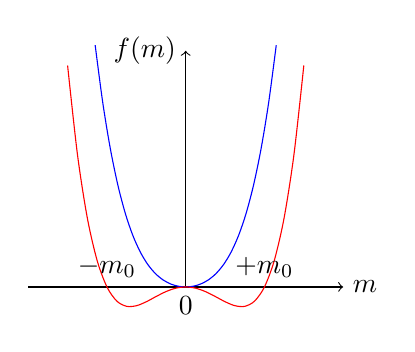
\begin{tikzpicture}
      \draw[->] (-2,0) -- (2,0) node[right] {$m$};
      \draw[->] (0,0) -- (0,3) node[left] {$f(m)$};
      \draw[domain=-1.15:1.15,smooth,variable=\x,blue] plot ({\x},{(\x)^2+(\x)^4});
      \draw[domain=-1.5:1.5,smooth,variable=\x,red] plot ({\x},{-(\x)^2+(\x)^4});
      \draw (0,0) node[below]{0};
    \draw (1,0) node[above]{$+m_0$};
    \draw (-1,0) node[above]{$-m_0$};
\end{tikzpicture}
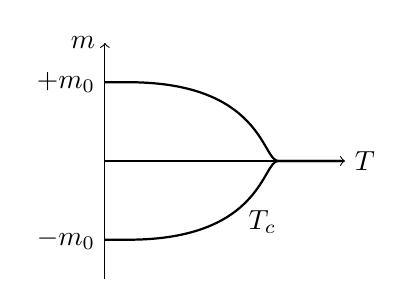
\begin{tikzpicture}
      \draw[->] (0,0) -- (3.05,0) node[right] {$T$};
      \draw[->] (0,-1.5) -- (0,1.5) node[left] {$m$};

    \draw [thick] (0, 1) -- (0.3, 1) .. controls (2, 1) and (2, 0) .. (2.2, 0) -- (3, 0);
    \draw [thick] (0, -1) -- (0.3, -1) .. controls (2, -1) and (2, 0) .. (2.2, 0) -- (3, 0);
    \draw (0,1) node[left]{$+m_0$};
    \draw (0,-1) node[left]{$-m_0$};
    \draw (2,-0.5) node[below]{$T_c$};
  \end{tikzpicture}
\end{center}
\begin{remarks}\leavevmode
\begin{enumerate}
    \item The expression 
$$m_0(T\sim T_c)=\pm\sqrt{3(T_c-T)/T}$$
is only valid close to $T_c$ when $m$ is small, and higher order terms $O(m^4)$ can be ignored.
    \item $f(m)$ is invariant under $\mathbb{Z}_2$ symmetry, i.e. $m\rightarrow -m$ leaves $f(m)$ invariant. This symmetry is inherited from the $S_i\rightarrow-S_i$ symmetry of the Ising model when $B=0$.
    \item For $T<T_c$, the system chooses one of the two states $m=\pm m_0$, i.e. the $\mathbb{Z}_2$ symmetry is spontaneously broken. Spontaneous symmetry breaking occurs if the symmetry of a system is not respected by the ground state.
\end{enumerate}
\end{remarks}
\begin{prop}
The heat capacity is discontinuous at $T=T_c$.
\end{prop}
\begin{proof}
The heat capacity (at constant $B=0$) is a response function, given by
$$C=\frac{\partial\langle E\rangle}{\partial T}=\beta^2\frac{\partial^2}{\partial\beta^2}\ln Z,\quad\langle E\rangle=-\frac{\partial}{\partial\beta}\ln Z$$
Bearing in mind the various $m_{\text{min}}$ (that minimizes the effective free energy) solutions obtained earlier, in the different regimes, we have 
$$f(m_{\text{min}})=
\left\{
        \begin{array}{ll}
      \frac{1}{2}(T-T_c)\times 0+\frac{1}{12}T\times 0\quad=0 & T>T_c \\
      \frac{1}{2}(T-T_c)\frac{3(T_c-T)}{T}+\frac{1}{12}T\frac{9(T_c-T)^2}{T^2}=-\frac{3}{4}\frac{(T_c-T)^2}{T} & T<T_c
      \end{array}
    \right.$$
Using $\ln Z\approx-\beta N f(m_{\text{min}})$ gives the heat capacity per particle to be
$$c=\frac{C}{N}=\frac{\beta^2}{N}\frac{\partial^2}{\partial\beta^2}(-\beta N f(m_{\text{min}}))=
\left\{
        \begin{array}{ll}
      0 & T\rightarrow T_c^+ \\
      \frac{3}{2} & T\rightarrow T_c^-
        \end{array}
    \right.$$
\end{proof}
\subsubsection{$B\neq 0$: a discontinuous phase transition}
\begin{defi}[First order phase transition]
At a first order phase transition, the order parameter changes discontinuously.
\end{defi}
\begin{prop}
For all temperatures $T$, the sign of $m$ is completely determined by the sign of $B$.
\end{prop}
\begin{proof}
The free energy is
$$f(m)\approx-Bm+\frac{1}{2}(T-T_c)m^2+\frac{1}{12}Tm^4+\dots$$
Two minima exist for low temperatures - one being metastable and another is a true ground state. 
$$0=\frac{\partial f(m)}{\partial m}=-B+(T-T_c)m+\frac{1}{3}Tm^3+\dots$$
$$0<\frac{\partial^2f(m)}{\partial m^2}=(T-T_c)+Tm^2+\dots$$
The metastable state disappears if the temperature increases above a certain value - the spinodal point. As we vary temperature $T$, the magnetization varies smoothly with asymptotic behaviour:
$$\lim_{T\rightarrow\infty}m=\frac{B}{T},\quad\lim_{T\rightarrow0}m=\pm1$$
\end{proof}
\begin{center}
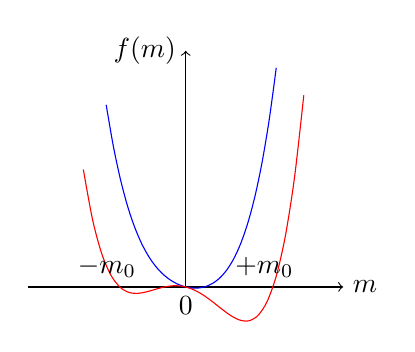
\begin{tikzpicture}
      \draw[->] (-2,0) -- (2,0) node[right] {$m$};
      \draw[->] (0,0) -- (0,3) node[left] {$f(m)$};
      \draw[domain=-1.01:1.15,smooth,variable=\x,blue] plot ({\x},{-0.25*\x+(\x)^2+(\x)^4});
      \draw[domain=-1.3:1.5,smooth,variable=\x,red] plot ({\x},{-0.25*\x-(\x)^2+(\x)^4});
      \draw (0,0) node[below]{0};
    \draw (1,0) node[above]{$+m_0$};
    \draw (-1,0) node[above]{$-m_0$};
\end{tikzpicture}
  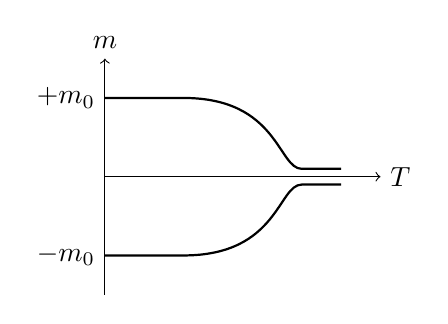
\begin{tikzpicture}
    \draw [->] (0, 0) -- (3.5, 0) node [right] {$T$};
    \draw [->] (0, -1.5) -- (0, 1.5) node [above] {$m$};

    \draw [thick] (0, 1) -- (1, 1) .. controls (2.2, 1) and (2.2, 0.1) .. (2.5, 0.1) -- (3, 0.1);
     \draw [thick] (0, -1) -- (1, -1) .. controls (2.2, -1) and (2.2, -0.1) .. (2.5, -0.1) -- (3, -0.1);
      \draw (0,1) node[left]{$+m_0$};
    \draw (0,-1) node[left]{$-m_0$};
  \end{tikzpicture}
\end{center}
\begin{prop}
For $T<T_c$, the magnetization $m$ (the order parameter) jumps discontinuously from $-m_0$ to $+m_0$ as $B$ flips from negative to positive. This is characteristic of a first order phase transition.
\end{prop}
\begin{proof}
Take the red curve from the previous diagram. The position of the true minima depends on the sign of $B$. If $B=0$, we obtain two minima, like earlier.
\end{proof}
\begin{remarks}
Draw $B$ against $T$. This line of first order phase transitions occurs at $B=0$ along $T>0$ axis and ends at a second order phase transition at $T = T_c$. This is referred to as the critical point. For $T>T_c$, we no longer experience a sign change in $m$ if the sign of $B$ changes.
\end{remarks}
\subsubsection{Close to Critical Point}
\begin{prop}
The magnetic susceptibility (another type of response function, i.e. $\chi=\frac{\partial m}{\partial B}|_T$) of the Ising model have the following behaviour near a critical point.
$$\chi\sim\frac{1}{|T-T_c|}$$
Close to the critical point $T\sim T_c$, $m$ scales like $m\sim\sgn(B)|B|^{1/3}$.
\end{prop}
\begin{proof}
Close to the critical point $T=T_c$,
$$f(m)\approx-Bm+\frac{1}{12}T_cm^4+\dots\implies \frac{\partial f}{\partial m}=0\implies m\sim B^{1/3},\quad B>0$$
and when $B<0$, $m\sim-|B|^{1/3}$. For $T>T_c$,
$$f(m)\approx-Bm+\frac{1}{2}(T-T_c)m^2+\dots\implies \frac{\partial f}{\partial m}=0\implies m\approx\frac{B}{T-T_c}\implies\chi=\frac{\partial m}{\partial B}\sim\frac{1}{T-T_c},\quad T\rightarrow T_c^+$$
For $T<T_c$, we can write minimum of $f$ as $m=m_0+\delta m$ for small $B$, and so to leading order in $B/T$, 
$$m\approx m_0+\frac{B}{2(T_c-T)}\implies\chi\sim\frac{1}{T_c-T},\quad T\rightarrow T_c^-$$
\end{proof}
\subsubsection{Validity of Mean Field Theory (MFT)}
\begin{enumerate}
    \item For $d=1$: MFT is completely wrong as there is supposed to be no phase transition.
    \item For $d=2,3$: The basic structure of the phase diagram looks right, but the details near the $T_c$ are wrong.
    \item For $d\geq4$: MFT gives the right answers.
\end{enumerate}
Similar stories for other systems:
\begin{enumerate}
    \item MFT fails completely for $d\leq d_l$, the lower critical dimension.
    \item MFT always works for $d\geq d_u$, the upper critical dimension.
    \item What about $d_l<d<d_u$? Often, those $d$'s are interesting.
\end{enumerate}
\begin{eg}[Critical Exponents]
In our MFT approach, we have seen that various quantities scale as power laws, as we approach the critical point. We first approach the critical point along the temperature axis ($B=0$):
$$m\sim(T_c-T)^\beta,\quad\beta=\frac{1}{2},\quad T<T_c$$
$$c\sim c_\pm|T-T_c|^{-\alpha},\quad\alpha=0\text{ (discontinuity)}$$
$$\chi\sim|T-T_c|^{-\gamma},\quad\gamma=1$$
To obtain the final exponent, we vary $B$ at $T=T_c$:
$$m\sim B^{1/\delta},\quad\delta=3$$
$\alpha,\beta,\gamma,\delta$ are called critical exponents.
\end{eg}
Compare MFT results with the true values for the Ising model in $d=2$ and 3:
\begin{table}[H]
\centering
\begin{tabular}{|l|l|l|l|l|}
\hline
      & MFT & d=2 & d=3         \\
      \hline
$\alpha$ & 0   & 0   & 0.1101...   \\
 \hline
$\beta$  & 1/2 & 1/8 & 0.3264...   \\
 \hline
$\gamma$ & 1   & 7/4 & 1.2371...   \\
 \hline
$\delta$ & 3   & 15  & 4.7898...  \\
\hline
\end{tabular}
\end{table}
\begin{remarks}
The critical exponents are only analytically worked out in $d=2$. $d=3$ is a numerical result, and no one has obtained an analytical solution for the 3D Ising model.
\end{remarks}
\subsubsection{Universality}
The liquid-gas transition shows many similarities to the Ising model. Again, a line of first-order phase transitions ending at a critical point. At fixed $p$, the volume per particle $v=V/N$ jumps discontinuously at a liquid-gas first-order phase transition. This suggests $v$ is an order parameter, analogous to $m$ in the ising model. using an equation of state (e.g. van der Waals equation in statistical physics) at the critical point:
$$v_{\text{gas}}-v_{\text{liquid}}\sim(T_c-T)^\beta,\quad\beta=\frac{1}{2},\quad T<T_c$$
$$v_{\text{gas}}-v_{\text{liquid}}\sim(p-p_c)^{1/\delta},\quad\delta=3,\quad p\rightarrow p_c^+$$
Analogous to the susceptibility, the compressibility (another response function) is
$$\kappa=-\frac{1}{v}\frac{\partial v}{\partial p}\bigg|_T\sim|T-T_c|^{-\gamma},\quad\gamma=1$$
$$C_V\sim C_\pm|T-T_c|^{-\alpha},\quad\alpha=0$$
The critical exponents ($\alpha=0,\beta=1/2,\gamma=1,\delta=3$) of liquid-gas transition are the same as the Ising model using MFT. None of these theoretical values, again, agree with experiment. But yet, the actual experimental measurements of the critical exponents agree with $d=3$ Ising.
\begin{defi}[Universality]
The critical point governs behaviour of many different physical systems. All memory of underlying microscopic physics is washed away. If two systems are governed by the same critical point, we say they live in the same universality class.
\end{defi}
\newpage
\subsection{Landau-Ginzburg Theory}
Due to universality, if we want to accurately describe the critical point, we need not concern ourselves with the messy details of any specific system. Instead, we should just search for the simplest model which gives the correct physics and work with that.\\[5pt]
What is the simplest model? The Landau approach – in which the configuration of the Ising model is reduced to a single number $m$ – is too coarse since it misses any spatial variation in the system. Spatial variations is important for critical points. Here we describe a simple generalisation of Landau’s ideas which allows the system to move away from a homogeneous state. 
\begin{defi}[Coarse graining]
To account for spatial variation, we consider $m$ as a field $m(\mathbf{x})$, i.e. a local order parameter. Start with a lattice with $N$ boxes and each of these boxes contains $N$' number of lattice sites, but the box side length $a$ is smaller than any other relevant length scale, so that $\mathbf{x}$ can be treated as continuous.
$$1<<N'<<N,\quad a<<\text{ other relevant length scales}$$
For each box, we define the average magnetisation 
$$m(\mathbf{x})=\frac{1}{N'}\sum_iS_i$$
where $\mathbf{x}$ denotes the centre of the box and the sum occurs over all the sites in the box. This kind of procedure in known as coarse-graining. $N'$ is large enough so $m\in[-1,1]$ is essentially continuous, but $m$ cannot vary on scales less than $a$, by construction.
\end{defi}
\begin{defi}[Partition function as a path integral]
Like before, the partition function is
$$Z=\sum_{m(\mathbf{x})}\sum_{\{S_i\}|m(\mathbf{x})}e^{-\beta E[S_i]}:=\sum_{m(\mathbf{x})}e^{-\beta F[m(\mathbf{x})]}$$
where the functional $F$ takes function $m(\mathbf{x})$ and outputs a number. The sum with index $\{S_i\}|m(\mathbf{x})$ is such that it is done over all $\{S_i\}$ such that the coarse graining gives $m(\mathbf{x})$. A further sum over all possible fields $m(\mathbf{x})$ is taken. Write $Z$ as a functional integral, also known as path integral
$$Z=\int e^{-\beta F[m(\mathbf{x})]}\mathcal{D}m(\mathbf{x})$$
The notation $\mathcal{D}m$ means that we should sum over all field configurations $m(\mathbf{x})$. 
\end{defi}
\begin{defi}[Landau Ginzburg free energy]
$F[m(\mathbf{x})]$ is called the Landau Ginzburg free energy, and it must have the following properties:
\begin{enumerate}
    \item locality: $f[m(\mathbf{x})]$ is a local function that depends on $m(\mathbf{x})$, $\boldsymbol{\nabla}m(\mathbf{x})$, $\nabla^2m(\mathbf{x})$;
    \item inherit symmetry of the system;
    \item analyticity (assume $f[m(\mathbf{x})]$ has a  Taylor series expansion).
\end{enumerate}
Further, if we are only interested in $m(\mathbf{x})$ that are slowly varying in space, then $\boldsymbol{\nabla}m$ terms are more important than $\nabla^2m$ terms, etc. $m(\mathbf{x})$ can be a generic order parameter.
\end{defi}
\begin{eg}[Ising model]
Since spins only affect their neighbours, $f[m(\mathbf{x})]$ is indeed local. The symmetries inherited from the Ising model are:
\begin{itemize}
    \item translation symmetry: no preference for a certain site;
    \item rotation symmetry: cannot have terms linear in the gradient like $\boldsymbol{\nabla}m$;
    \item $\mathbb{Z}_2$ symmetry when $B=0$: $f[m(\mathbf{x})]$ must only have even powers in $m$.
\end{itemize}
With all these considerations, the most general free energy when $B=0$ is
$$F[m(\mathbf{x})]=\int\bigg(\frac{1}{2}\alpha_2(T)m^2+\frac{1}{4}\alpha_4(T)m^4+\frac{1}{2}\gamma(T)(\boldsymbol{\nabla}m)^2+\dots\bigg)d^dx$$
In general, it is hard to compute coefficients $\alpha_2(T)$, $\alpha_4(T)$ and $\gamma(T)$ from first principles. Fortunately, the exact form of these functions are not necessary, all we need are:
\begin{enumerate}
    \item $\alpha_4(T),\gamma(T)>0$
    \item $\alpha_2(T)$ changes sign at $T=T_c$.
\end{enumerate}
\end{eg}
\begin{eg}
From MFT, we expect
$$\alpha_2(T)\sim T-T_c,\quad\alpha_4(T)\sim\frac{1}{3}T$$
\end{eg}
The first attempt in solving this path integral would be to use the saddle point method, i.e. assume the path integral is dominated by the configurations which minimize $F[m(\mathbf{x})]$. 
\begin{prop}
MFT is a saddle point approximation of the Landau-Ginzburg theory.
\end{prop}
\begin{proof}
The first-order variation in free energy from a variation $m(\mathbf{x})+\delta m(\mathbf{x})$ is
\begin{align}
    \delta F&=\int[\alpha_2m\delta m+\alpha_4m^3\delta m+\gamma(\boldsymbol{\nabla}m)\cdot(\boldsymbol{\nabla}\delta m)+O((\delta m)^2)]~d^dx\nonumber\\&=\int[\alpha_2m+\alpha_4m^3-\gamma\nabla^2m]\delta m~d^dx+\dots\nonumber
\end{align}
where we integrated by parts. If the original field configuration $m(\mathbf{x})$ was a minimum of the free energy, then it satisfies the Euler-Lagrange equations. Hence, the minima occurs when $\gamma\nabla^2m=\alpha_2m+\alpha_4m^3$. The simplest solutions to this equation have m constant, i.e. solve $0=\alpha_2m+\alpha_4m^3$. This recovers our earlier results from Landau theory, i.e. when $T>T_c$, $\alpha_2>0\implies m=0$; when $T<T_c$, $\alpha_2<0\implies m=\pm m_0=\pm\sqrt{-\alpha_2/\alpha_4}=\pm\sqrt{3(T_c-T)/T}$.
\end{proof}
\begin{defi}[Domain Wall]
A domain wall is an interface between two regions of space - one with $m=+m_0$ and the other with $m=-m_0$. This occurs for $T<T_c$ where there are two ground states $m=\pm m_0$. 
\end{defi}
\begin{remarks}
Whenever we have a Landau-Ginzburg theory characterised by a discrete symmetry, then the ordered phase will have a number of degenerate, disconnected ground states which spontaneously break the symmetry. In all such cases, the lower critical dimension is $d_l = 1$ and in all cases the underlying reason is the same: fluctuations of domain walls (unsuppressed because of entropy) will take us from one ground state to another and destroy the ordered phase. It is said that the domain walls proliferate.
\end{remarks}
\subsection{Continuous symmetry models [non-examinable]}
This topic is introduced to link the idea of phase transition with symmetry breaking. Phases of matter are characterized by two symmetry groups.
\begin{itemize}
    \item $G$ is the symmetry of the free energy,
    \item $H$ is the symmetry of the ground state.
\end{itemize}
\begin{eg}
For the Ising model, $G=\mathbb{Z}_2$. When $B=0$, this maps $\phi\rightarrow-\phi$. In the disordered phase, $H=\mathbb{Z}_2$. In the ordered phase, we must choose one of two ground states, $H=\phi$ (spontaneous symmetry breaking). But when $B\neq 0$, $G=\phi$. Along the line of first order phase transitions, there is an emergent $\mathbb{Z}_2$ symmetry, which is spontaneously broken to $H=\phi$.
\end{eg}
\begin{remarks}
Whenever a discrete symmetry group is spontaneously broken, it results in multiple ground states. One can move from one ground state to another by acting with the broken generators of $G$.
\end{remarks}
\begin{remarks}
The idea of symmetry is useful in characterising nearly all phases of matter. In each case, one should first determine an order parameter and a symmetry group $G$ under which it transforms. Next, write down the most general Landau-Ginzburg free energy, subject to the requirement that it is invariant under $G$. The different phases of matter within this class are characterised by the group $H$ preserved by the ground state. This is a useful classification because:
\begin{itemize}
    \item for fixed $G$, change of $H$ indicates phase transition
    \item nature of critical point (i.e. universality class) is determined by $G$.
\end{itemize}
\end{remarks}
\begin{defi}[$O(N)$ models]
Consider a system where the order parameter is an $N$-dimensional vector:
$$\boldsymbol{\phi}(\mathbf{x})=(\phi_1(\mathbf{x}),\phi_2(\mathbf{x}),\dots,\phi_N(\mathbf{x}))$$
We will construct a free energy that is invariant under $O(N)$ symmetry. $\phi_a(\mathbf{x})\rightarrow R^b_a\phi_b(\mathbf{x})$ with $R^TR=1\implies R\in O(N)$ and $a,b=1,\dots N$.
\end{defi}
The free energy (with terms invariant under $O(N)$) is
$$F[\boldsymbol{\phi}(\mathbf{x})]=\int\bigg[\frac{\gamma}{2}\boldsymbol{\nabla}\boldsymbol{\phi}\cdot\boldsymbol{\nabla}\boldsymbol{\phi}+\frac{\mu^2}{2}\boldsymbol{\phi}\cdot\boldsymbol{\phi}+g(\boldsymbol{\phi}\cdot\boldsymbol{\phi})^2+\dots\bigg]d^dx$$
\begin{eg}\leavevmode
\begin{enumerate}
    \item $O(1)$: $\mathbb{Z}_2$ symmetry in Ising model
    \item $O(2)$: XY-model. Write the two real scalar fields as a single complex field $\psi(\mathbf{x})=\phi_1(\mathbf{x})+i\phi_2(\mathbf{x})$. The free energy consists all terms which are invariant under $U(1)$ global phase rotations, i.e. $\psi\rightarrow e^{i\alpha}\phi$. 
    $$F[\psi(\mathbf{x})]=\int\bigg[\frac{\gamma}{2}\boldsymbol{\nabla}\psi^*\cdot\boldsymbol{\nabla}\psi+\frac{\mu^2}{2}|\psi|^2+g|\psi|^4+\dots\bigg]d^dx$$
    It describes magnets when spin is free to rotate in a plane. The energy is 
    $$E=-J\sum_{\langle i,j\rangle}\mathbf{s_i}\cdot\mathbf{s_j}=-J\sum_{\langle ij\rangle}\cos(\theta_i-\theta_j)$$
    where $\mathbf{s_i}$ is a 2D unit vector. Again $\mathbf{B}$ will break the $O(2)$ symmetry.
    \item Another $O(2)$: This also describes superfluid and BECs. The order parameter $\psi$ is related to the off-diagonal long-range order in the one-particle density matrix. The saddle point of the free energy leads to the equation of motion - the Gross-Pitaevskii equation.
    \item $O(3)$: Heisenberg model. This time, $\mathbf{s_i}$ are 3D unit vectors.
\end{enumerate}
\end{eg}
\subsubsection{Heisenberg Model}
When there is no external field, the Heisenberg Hamiltonian is symmetric under generic global rotations of the spins. If an ordered phase develops where $\langle S_i\rangle\neq 0$, it breaks the symmetry by choosing a direction. 
\begin{prop}
The self-consistent mean-field solution of the Heisenberg model is
$$s=-\frac{1}{2q\beta Js+\beta B}+\coth(2q\beta Js+\beta B)$$
where $q$ is the number of nearest neighbours.
\end{prop}
\begin{proof}
The Heisenberg Hamiltonian in the presence of an external field is
$$H=-\frac{J}{2}\sum_{\langle i,j\rangle}\mathbf{S_i}\cdot\mathbf{S_j}-B\sum_i\mathbf{S_i}\cdot\mathbf{\hat{z}},\quad J>0,\quad\mathbf{S}_i=\begin{pmatrix}\sin\theta\cos\phi\\\sin\theta\sin\phi\\\cos\theta\\\end{pmatrix}$$
In the mean field approximation of small fluctuations about the average spin value $|\mathbf{S_i}-\mathbf{S}|<<1$, expand the energy to linear order: $H\approx-(2qJs+B)\sum_i\hat{z}\cdot\mathbf{S_i}$. The approximated canonical partition function is
$$Z=\sum_{\{S_i\}}e^{-\beta H(\{S_i\})}\approx (2\pi)^N\bigg[\int_{-1}^1 e^{(2q\beta Js+\beta B)x}\bigg]^N,\quad x=\cos\theta$$
The average spin is
$$s=\langle\mathbf{S_i}\cdot\hat{z}\rangle=\frac{(\pi)^N}{Z}\bigg[\int_{-1}^1e^{(2q\beta Js+\beta B)x}dx\bigg]^{N-1}\bigg[\int_{-1}^1xe^{(2q\beta Js+\beta B)x}dx\bigg]=-\frac{1}{2q\beta Js+\beta B}+\coth(2q\beta Js+\beta B)$$
\end{proof}
\begin{remarks}
The critical exponents can be shown to be the same as when MFT is used for the Ising model.
\end{remarks}
\subsubsection{Goldstone bosons again [non-examinable]}
With a continuous symmetry, we have an infinite number of choices after spontaneous symmetry breaking. The minimum of the free energy constrains only the magnitude of $\boldsymbol{\phi}$ which is given by
$$\langle|\boldsymbol{\phi}|\rangle=M_0=\sqrt{-\mu^2/4g}$$
However, minimizing the free energy does not determine the direction of $\boldsymbol{\phi}$. We are left with a space of ground states which is the sphere $\mathcal{S}^{N-1}$. Each point on the sphere, parameterises the direction of $\boldsymbol{\phi}$ and has the same energy. This infinitely degenerate choice of ground states means that we can consider configurations in which we stay within the space of ground states, but the direction varies in space. For such configurations, the part of the free energy $f(\boldsymbol{\phi})=\frac{\mu^2}{2}|\boldsymbol{\phi}|^2+g|\boldsymbol{\phi}|^4+\dots$ remains minimized, but we pick up contributions from the gradient terms $|\boldsymbol{\nabla}\boldsymbol{\phi}|^2$. However, we can always lower this free energy by making the `twisting' variation take place over longer and longer distances.
\begin{thm}[Goldstone's theorem]
In any system, the spontaneous breaking of a continuous symmetry gives rise to a gapless excitation, i.e. Goldstone boson. The space of ground states has dimension $N-1$.
\end{thm}
\begin{remarks}
In general, an excitation whose energy cost vanishes as the wavelength goes to infinity is referred to as a gapless mode. These are to be contrasted with gapped excitations whose energy remains finite in this limit. Gapless excitations often dominate the low-temperature behaviour of a system, where they are the only excitations that are not Boltzmann suppressed. In many systems, these gapless modes arise from the breaking of some symmetry.
\end{remarks}
\begin{eg}
In the context of the Heisenberg model, Nambu-Goldstone bosons are called spin waves. Another example - phonons in a solid can be thought of as Goldstone bosons for broken translational symmetry.
\end{eg}
\begin{eg}[XY model]
In the ordered phase, we get a so-called Mexican hat potential, which has a circle $\mathcal{S}^1$ of minima. It is useful to decompose the field as $\psi(\mathbf{x})=M(\mathbf{x})e^{i\theta(\mathbf{x})}$. In the ground state, $M=M_0=\sqrt{-\mu^2/4g}$, while $\theta$ is arbitrary. Write $M(\mathbf{x})=M_0+\tilde{M}(\mathbf{x})$, then the free energy has the expansion
$$F[M,\theta]=\int\frac{\gamma}{2}(\boldsymbol{\nabla}\tilde{M})^2+|\mu|^2\tilde{M}^2+g\tilde{M}^4+\dots+\frac{\gamma}{2}M_0^2(\boldsymbol{\nabla}\theta)^2+\gamma M_0\tilde{M}(\boldsymbol{\nabla}\theta)^2+\dots$$
Here, the Goldstone boson is $\theta(\mathbf{x})$ and there are only derivative interactions.
\end{eg}
\begin{eg}[Heisenberg model]
For the $O(3)$ model, we decompose the field in spherical polar coordinates
$$\boldsymbol{\phi}=M\begin{pmatrix}\sin\theta\cos\phi\\\sin\theta\sin\phi\\\cos\theta\\\end{pmatrix},\quad\theta\in[0,\pi),~\phi\in[0,2\pi)$$
In the ordered phase, we have $M=M_0\neq 0$, with $\theta$ and $\phi$ arbitrary. The free energy is
$$F[M,\theta,\phi]=\int\frac{\gamma}{2}(\boldsymbol{\nabla}\tilde{M})^2+|\mu|^2\tilde{M}^2+g\tilde{M}^4+\dots+\frac{\gamma}{2}M_0^2[(\boldsymbol{\nabla}\theta)^2+\sin^2\theta(\boldsymbol{\nabla}\phi)^2]+\dots$$
Here, $\theta$ and $\phi$ are the two Goldstone modes, which again have only derivative interactions. But this time, they interact with each other. The metric on the two-sphere appears in the gradient terms, i.e. the geometry of the minima ($\mathcal{S}^2$ by Goldstone's theorem) gets imprinted on the dynamics of the Goldstone modes.
\end{eg}
\newpage
\subsection{Problems}
\begin{qns}
Mean field theory becomes exact for the Ising model provided the same interaction acts between all pairs of spins, not just nearest neighbours. Consider a system with $N$ $(>>1)$ spins, with an interaction between each pair of spins proportional to $1/N$.
\begin{enumerate}[label=(\alph*)]
\item  Show that that the overall energy is proportional to $N$.
\item The Hamiltonian of the model is 
$$H=-\frac{J}{N}\sum_{i,j}s_is_j,\quad s_i=\pm1,\quad s_i^2=1$$
where $J$ is a constant and the sum runs over all pairs $(i, j)$, not just over nearest neighbours. Show that 
$$H=-\frac{J}{2N}\bigg[\bigg(\sum_{i=1}^Ns_i\bigg)^2-N\bigg]$$
\item Let $m=\langle s\rangle$ be the magnetisation per spin, i.e. $m=\frac{1}{N}\sum_i s_i$ with $−1\leq m\leq +1$. Show that the degeneracy of the state with magnetisation $m$ is
$$W(m)=\frac{N!}{(\frac{1}{2}N(1+m))!(\frac{1}{2}N(1-m))!}$$
\item Show that the partition function may be written
$$Z=\sum_mW(m)e^{-H(m)/k_BT}$$
where $H(m)$ is the value of the Hamiltonian when the magnetisation is $m$. Evaluate $Z$ by using Stirling’s approximation, $n!\approx n^ne^{-n}$ for large $n$, and by showing that in the above expression for $Z$ the sum over $m$ may be replaced by its largest term. Show that this term is given by the maximum of the function
$$-F=Jm^2-k_BT[(1+m)\ln(1+m)+(1-m)\ln(1-m)]$$
Sketch $−F$ as a function of $m$ for various values of $T$ (i.e. both large and small).
\item By looking for the maximum of $−F$, prove that there is a phase transition, and calculate the critical temperature $T_c$. In recovering the equation of mean-field theory given in the lectures, it may prove useful to note that $\ln[(1+x)/(1−x)] = 2\tanh^{-1}(x)$. What is the sign of $F''(m_0)$ where $m_0$ is the magnetisation?
\item For $m\rightarrow 0$, show that $F$ assumes the form anticipated by Landau theory and given in the lecture notes, namely
$$F(T)=F_0+\alpha(T)m^2+\frac{1}{2}\beta(T)m^4$$
where $\alpha(T_c)=0$. Evaluate $\alpha(T)$ and $\beta(T)$.
\item Generalise to the case of a uniform external field $B$.
\end{enumerate}
\end{qns}
\begin{ans}\leavevmode
\begin{enumerate}[label=(\alph*)]
\item Here, we assume the same interaction between all pairs of spins ($i<j$ to prevent double counting), not just the nearest neighbours. As a result, the system clearly has translation invariance and is scale free. The energy is $E=\langle H\rangle$, and the ensemble average is a constant value $\mathcal{E}$ independent of $i$ and $j$.
$$E=-\frac{J}{N}\sum_{i<j}s_is_j=-\frac{J}{N}N^2\mathcal{E}=-JN\mathcal{E}\propto N$$
where the given interaction is proportional to $1/N$.
\item The Hamiltonian is
$$H=-\frac{J}{N}\sum_{i<j}s_is_j=-\frac{J}{N}\frac{1}{2}\bigg[\bigg(\sum_{i=1}^Ns_i\bigg)^2-\sum_{i=1}^Ns_i^2\bigg]=-\frac{J}{2N}\bigg[\bigg(\sum_{i=1}^Ns_i\bigg)^2-N\bigg]$$
where we used $s_i^2=1$ $\forall i$. The identity
$$2\sum_{i<j}s_is_j=\bigg(\sum_{i=1}^Ns_i\bigg)^2-\sum_{i=1}^Ns_i^2$$
may be proven by induction.
\item Writing in terms of the magnetization, the Hamiltonian is
$$H=-\frac{J}{2N}\bigg[(mN)^2-N\bigg]=-\frac{1}{2}Jm^2N+\frac{J}{2}$$
We may drop the unimportant constant. All configurations $\{s_i\}$ with the same magnetization $m$ are thus energetically degenerate. We have
$$mN=N^+-N^-=N^+-(N-N^+)\implies N^+=N\frac{1}{2}(1+m)$$
The total number of such configurations is
$$W(m)=~^NC_{N^+}=\frac{N!}{N^+!(N-N^+)!}=\frac{N!}{[N(1+m)/2]![N(1-m)/2]!}$$
where we choose $N^+$ out of the $N$ total spins to be pointing up. 
\item The partition function is
$$Z=\sum_{\{s_i\}_{i=1}^N}e^{-H/k_BT}=\sum_me^{-H(m)/k_BT}\bigg(\sum_{\{s_i\}|m}1\bigg)=\sum_m W(m)e^{-H(m)/k_BT}$$
where $\{s_i\}|m$ refers to all ensemble of configurations $\{s_i\}$ with the same magnetization $m$. Use Stirling's approximation for large $n$: $n!\approx n^ne^{-n}$. Then, the degeneracy is 
\begin{align}
W(m)&\approx\frac{N^Ne^{-N}}{[N(1+m)/2]^{N(1+m)/2}e^{-N(1+m)/2}[N(1-m)/2]^{N(1-m)/2}e^{-N(1-m)/2}}\nonumber\\&=\bigg[\bigg(\frac{1+m}{2}\bigg)^{(1+m)/2}\bigg(\frac{1-m}{2}\bigg)^{(1-m)/2}\bigg]^{-N}\nonumber\\&=\exp\bigg[-N\bigg(\frac{1+m}{2}\ln\frac{1+m}{2}+\frac{1-m}{2}\ln\frac{1-m}{2}\bigg)\bigg]\nonumber
\end{align}
and hence the partition function is 
$$Z=\sum_m\exp\bigg\{\frac{N}{2k_BT}(Jm^2-k_BT[(1+m)\ln(1+m)+(1-m)\ln(1-m)])\bigg\}=\sum_me^{-NF(m)/2k_BT}$$
where $H(m)=-\frac{1}{2}JNm^2$. The discarded constant is unimportant since $Z$ is unique up to a multiplicative constant. We also further omitted another unimportant constant $e^{N\ln 2}$. The finite sum is bounded below by the largest element, and bounded above by having each element to be the maximum, so
$$e^{-NF_{\text{min}}/2k_BT}\leq Z\leq Ne^{-F_{\text{min}}N/2k_BT}\implies-\frac{F_{\text{min}}}{2k_BT}\leq\frac{\ln Z}{N}\leq\frac{\ln N}{N}-\frac{F_{\text{min}}}{2k_BT}$$
For large $N$, $\frac{\ln N}{N}\rightarrow 0$ and so $\frac{\ln Z}{N}\rightarrow -\frac{F_{\text{min}}}{2k_BT}$. Hence, $Z$ is asymptotically bounded by the largest value of the elements in the summation over $m$, i.e. the maximum of 
$$-F(m)=Jm^2-k_BT[(1+m)\ln(1+m)+(1-m)\ln(1-m)]$$
We plot $-F(m)$ against $m$ for $m\in(-1,1)$, $J=1$ and $k_BT=0.7,1.0,1.3$ (blue, black, red respectively).
\begin{center}
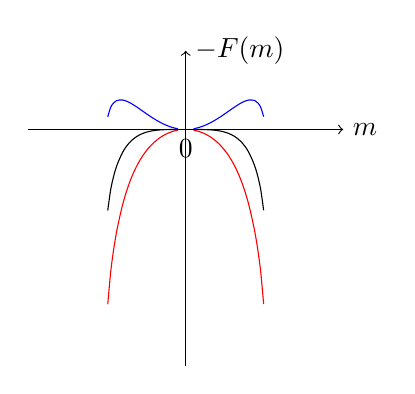
\begin{tikzpicture}
      \draw[->] (-2,0) -- (2,0) node[right] {$m$};
      \draw[->] (0,-3) -- (0,1) node [right] {$-F(m)$};
      \draw[domain=-0.99:-0.1,smooth,variable=\x,black] plot ({\x},{3*(\x*\x-1*((1+\x)*ln(1+\x)+(1-\x)*ln(1-\x)))});
      \draw[domain=0.1:0.99,smooth,variable=\x,black] plot ({\x},{3*(\x*\x-1*((1+\x)*ln(1+\x)+(1-\x)*ln(1-\x)))});
      
      \draw[domain=-0.99:-0.1,smooth,variable=\x,blue] plot ({\x},{3*(\x*\x-0.7*((1+\x)*ln(1+\x)+(1-\x)*ln(1-\x)))});
      \draw[domain=0.1:0.99,smooth,variable=\x,blue] plot ({\x},{3*(\x*\x-0.7*((1+\x)*ln(1+\x)+(1-\x)*ln(1-\x)))});
      
      \draw[domain=-0.99:-0.1,smooth,variable=\x,red] plot ({\x},{3*(\x*\x-1.3*((1+\x)*ln(1+\x)+(1-\x)*ln(1-\x)))});
      \draw[domain=0.1:0.99,smooth,variable=\x,red] plot ({\x},{3*(\x*\x-1.3*((1+\x)*ln(1+\x)+(1-\x)*ln(1-\x)))});
      \draw (0,0) node[below]{0};
\end{tikzpicture}
\end{center}
\item Maximum of $-F(m)$:
$$0=-\frac{dF(m)}{dm}=2Jm-k_BT\ln\frac{1+m}{1-m}\implies\tanh\frac{Jm}{k_BT}=m$$
where we recover the mean field result from the suggested identity.
\begin{center}
\begin{tikzpicture}
      \draw[->] (-4,0) -- (4,0) node[right] {$m$};
      \draw[->] (0,-2.5) -- (0,2.5) ;
      \draw[domain=-3:3,smooth,variable=\x,black] plot ({\x},{tanh(\x)});
      \draw[domain=-3:3,smooth,variable=\x,red] plot ({\x},{tanh(2*(\x))});
      \draw[domain=-3:3,smooth,variable=\x,blue] plot ({\x},{tanh(0.5*(\x))});
      \draw[domain=-2:2,smooth,variable=\x,black] plot ({\x},{\x});
      \draw (0,0) node[below]{0};
    \draw (1,0) node[above]{$+m_0$};
    \draw (-1,0) node[above]{$-m_0$};
\end{tikzpicture}
\end{center}
A solution at $m=0$ always exists. If the slope of the hyperbolic tangent at $m=0$ is smaller than unity, i.e. $J<k_BT$, no further solutions and so $m=0$ is indeed a maximum. If the slope is larger than unity, i.e. $J>k_BT$, then two more solutions appear which are equal maxima of $-F(m)$ at $m=\pm m_0\neq 0$, whereas $m=0$ becomes a minimum. This is characteristic of the phenomenon of spontaneous symmetry breaking.
$$\frac{d^2F(m)}{dm^2}=2J-\frac{k_BT}{1+m}-\frac{k_BT}{1-m}=2J-\frac{k_BT(1-m+1+m)}{1-m^2}=2J-2k_BT\cosh^2\frac{Jm}{k_BT}$$
As $0\leq 1-m^2\leq 1$ for $J<k_BT$, $\frac{d^2F(m)}{dm^2}<0$ $\forall m$, i.e. $F(m)$ has a maximum. At $J=k_BT$, $\frac{d^2F(m)}{dm^2}=0$ at $m=0$ (typical of a second order phase transition) and it is negative elsewhere. For $J>k_BT$, $\frac{d^2F(m)}{dm^2}>0$ $\forall m\approx 0$ (minimum) and $\frac{d^2F(m)}{dm^2}<0$ $\forall m\approx\pm1$ (maximum).
\item Taylor expand for small $m$:
\begin{align}
    -F(m)&=Jm^2-k_BT[(1+m)\ln(1+m)+(1-m)\ln(1-m)]\nonumber\\&\approx Jm^2-k_BT\bigg(m+\frac{m^2}{2}-\frac{m^3}{6}+\frac{m^4}{12}\bigg)-k_BT\bigg(-m+\frac{m^2}{2}+\frac{m^3}{6}+\frac{m^4}{12}\bigg)\nonumber\\\implies F(m)&\approx-Jm^2+k_BT\bigg(m^2+\frac{m^4}{6}\bigg)+O(m^5)\nonumber
\end{align}
and so $\alpha(T)=k_BT-J=k_B(T-T_c)$, $\beta(T)=\frac{1}{3}k_BT$. $\alpha(T_c)=0$ indeed, with $\alpha>0$ above $m=0$ and $\alpha<0$ below $m=\pm m_0$.
\item The Hamiltonian is now $H=-\frac{J}{2}Nm^2-BNm$, unique up to some irrelevant constant. The spin configuration sitll depends only on magnetization $m$, so the previous discussion holds. The self-consistent solution is now
$$0=-\frac{dF(m)}{dm}=2Jm+B-k_BT\ln\frac{1+m}{1-m}\implies\tanh\frac{Jm+0.5B}{k_BT}=m$$
The point where the hyperbolic tangent vanishes is shifted to a negative value of $m=-B/2J$. For large temperature, $k_BT>J$, using a graphical solution, one can readily observe that the shift results in the intersection with $m$ moving from $m=0$ to a finite $m>0$. As the temperature is lowered, eventually two further solutions of the equation appear. The former single solution becomes increasingly larger and stays as the maximum at all temperatures. The two new solutions are a secondary maximum and a minimum respectively. The applied $B$ field explicitly breaks the symmetry of the system, and removes any trace of the thermodynamic transition.
\end{enumerate}
\end{ans}
\begin{qns}
The Landau free energy expansion for a uniaxial ferromagnet in a magnetic field can be written as
$$F=F_0-hm+\frac{a}{2}m^2+\frac{b}{4}m^4$$
where $m$ is the magnetisation of the system and $h$ represents an externally applied magnetic field.
\begin{enumerate}[label=(\alph*)]
\item Briefly discuss the origin of this expansion and what you know a priori about (some of) the terms and their coefficients.
\item Define and compute the exponent $\delta$ along the critical isotherm.
\item Compute the susceptibility $\chi=(\partial m/\partial h)|_{h=0}$ as a function of $t = (T − T_c)/T_c$ both above ($t > 0$) and below ($t < 0$) the transition. Show that
$$\lim_{t\rightarrow 0^+}\frac{\chi(t)}{\chi(-t)}=2$$
\item Add the term $dm^3/3$ to the free energy $F$ for a generic real parameter $d$ and set $h = 0$. Discuss how the nature of the ordering transition is affected.
\end{enumerate}
\end{qns}
\begin{ans}\leavevmode
\begin{enumerate}[label=(\alph*)]
\item Phase transitions occur when a new state (ordered phase) develops from the disordered phase. This is characterized by an order parameter, say the magnetization in an Ising model. The Landau-Ginzburg theory provides a phenomenological description of the critical phenomena based on an appropriately coarse-grained order parameter $m$. Due to universality, it is constructed on the basis of symmetries rather than precise knowledge of the microscopic properties of the system.\\[5pt]
Near the transition temperature, where the order parameter vanishes, one can expand the Landau-Ginzburg free energy in powers of $m$ and its derivatives. The latter often penalize spatial variations of the parameter $m$ and allow us to further simplify the free energy expansion by considering the case of uniform $m$.\\[5pt]
For $F$ to be bounded from below, $b>0$ ($b=0$ is allowed if $a>0$). Linear term in $m$ due to externally applied $B$ field. A transition in the free energy occurs when $a$ changes sign, i.e. $a(T_c)=0$.
\item The magnetisation of the system scales like a power law of the applied field along the critical isotherm (for small fields), with an exponent $1/\delta$. Along the critical isotherm $T=T_c$,
$$a(T_c=0)\implies F(T_c)=F_0-hm+\frac{b}{4}m^4$$
Equilibrium $m$ is obtained from $\frac{\partial F}{\partial m}=0$:
$$0=\frac{\partial F}{\partial m}(T=T_c)=-h+bm^3\implies m=\bigg(\frac{h}{b}\bigg)^{1/3}\implies\delta=1/3$$
\item The equilibrium occurs at
$$0=\frac{\partial F(T)}{\partial m}=-h+a(T)m+b(T)m^3$$
To find the susceptibility $\chi=(\frac{\partial m}{\partial h})|_{h=0}$, we differentiate with respect to $h$:
$$0=\frac{\partial^2F(T)}{\partial h\partial m}=-1+a(T)\frac{\partial m}{\partial h}+3b(T)m^2\frac{\partial m}{\partial h}\implies\chi=\frac{\partial m}{\partial h}=\frac{1}{a(T)+3b(T)m^2}$$
This is true $\forall h$, inclusive of $h=0$. For $t>0$, above the transition so $T>T_c$, $m=0\implies\chi=1/a(T)$. For $t<0$, $m\neq 0$, so
$$b(T)m^2=\frac{h-a(T)m}{m}\implies\chi=\frac{1}{a(T)+3(h/m-a(T))}\bigg|_{h=0}=-\frac{1}{2a(T)}=\frac{1}{2|a(T)|}$$
where $a(T)<0$ for $T<T_c$. Hence,
$$\lim_{t\rightarrow 0^+}\frac{\chi(t)}{\chi(-t)}=\lim_{t\rightarrow 0^+}\frac{2|a(-t)|}{a(t)}=\lim_{t\rightarrow 0^+}2=2$$
where we used L'Hopital rule since $a(T)\propto t=\frac{T-T_c}{T_c}$ for $T$ close to $T_c$.
\item The free energy is now
$$F=F_0+\frac{a}{2}m^2+\frac{d}{3}m^3+\frac{b}{4}m^4$$
The equilibrium magnetization occurs at
$$0=\frac{\partial F}{\partial m}=am+dm^2+bm^3\implies m=0,\quad m_\pm=\frac{-d\pm\sqrt{d^2-4ab}}{2b}$$
where $d^2>4ab$ since $m\in\mathbb{R}$. To determine whether this equilibrium is a maximum or minimum:
$$\frac{\partial^2F}{\partial m^2}=a+2dm+3bm^2$$
The sign of $F''(m)$ is controlled by the sign of $a$ at $m=0$.
\begin{itemize}
    \item If $a<0$, $m=0$ is a maximum. The other two solutions $m_\pm$ must be minima given $F(m)\rightarrow+\infty$ for $m\rightarrow\pm\infty$.
    \item If $a>0$, $m=0$ is a minimum. If $d$ is small, $m=0$ remains as global minimum. If not, $m=0$ is a local minimum.
\end{itemize}
Similar to the case $d=0$, the sign of $a$ drives a transition from a state with $m=0$ to a state with $m\neq 0$. The cubic term introduces two major changes:
\begin{itemize}
    \item symmetry in ordered phase is broken explicitly, i.e. $F(m_-)<F(m_+)$
    \item change in order parameter across the critical point $a=0$ is discontinuous, hence the transition has become first order.
\end{itemize}
\end{enumerate}
\end{ans}
\newpage
\begin{qns}
Consider the Landau free energy expansion of a system with complex order parameter $\phi(x)$ in 1D:
$$\beta H=\int fdx=\int\bigg[a\phi^*\phi+\frac{1}{2}(\phi^*\phi)^2+c(\partial_x\phi^*)(\partial_x\phi)+(\partial_x^2\phi^*)(\partial_x^2\phi)\bigg]dx$$
with the coefficients $a,c$ real.
\begin{enumerate}[label=(\alph*)]
\item When $c > 0$, this is equivalent to the free energy expected for an Ising ferromagnet discussed in the lecture notes, except that the order parameter is now complex. Find the physical state of the system as a function of the coefficients in the free energy and discuss the nature of the phase transition.\\[5pt]
What type of symmetry is spontaneously broken at this transition (assume $c > 0$)?\\[5pt]
Compute the dependence of the order parameter on the coefficient $a$ close to the transition, in the ordered phase.
\item Compute the behaviour of the zero-field magnetic susceptibility $\chi = (\partial\phi/\partial B)|_{B=0}$ close to the transition (both above and below). Once again, assume $c > 0$. It is convenient here to consider the susceptibility in response to a magnetic field $B$ pointing in the direction of the real axis in the complex $\phi$ plane. With this choice, you can take $\phi$ to be real in the expression for the free energy given above.
\item Consider then the general case where $c$ is allowed to take on negative as well as positive values. Assume that the order parameter takes the form $\phi(x)=\phi_0e^{i(kx+\delta)}$, where $\phi_0>0$, $k$ and $\delta$ are real constants. Find the values that these constants need to take in order to minimize the free energy, as a function of the coefficients $a$ and $c$. Hint: substitute the given form for $\phi(x)$ into the free energy
$$f|_{\phi(x)=\phi_0e^{i(kx+\delta)}}=a\phi_0^2+\frac{1}{2}\phi_0^4+ck^2\phi_0^2+k^4\phi_0^2$$ 
obtain the location of the extrema using partial derivatives with respect to $\phi_0$ and $k$; finally, compare the values of the free energy at these extrema to find which is the actual absolute minimum.\\[5pt]
What happens to the dependence on $\delta$? How does this relate to the type of symmetry that is spontaneously broken across the transition considered in part (b) above?
\item Using the information obtained in part (c), show that the phase transition lines (or phase boundaries) in the ac plane look like
\begin{figure}[H]
    \centering
    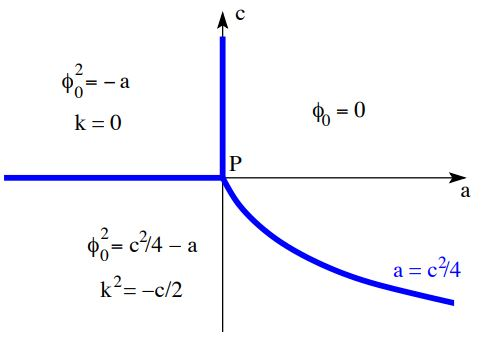
\includegraphics[scale=0.65]{TP1_Q3_PT.JPG}
\end{figure}
The point P where three transition lines meet is called a tricritical point. Consider the case $a = c$ and obtain how the order parameter behaves as a function of $c < 0$ close to the tricritical point P ($c = 0$). Consider then the case $a = 0$, $c < 0$, and compute how the order parameter behaves as a function of $c$ on approaching the same tricritical point P. Do you find the same exponents $\beta$, $\phi_0\sim(-c)^\beta$ in the two cases? (Recall that $|c|$ is small close to the critical point.)
\end{enumerate}
\end{qns}
\begin{ans}\leavevmode
\begin{enumerate}[label=(\alph*)]
\item The physical state of the system is obtained by minimizing the free energy. When $c>0$, this is minimized by a uniformly constant order parameter $\phi(x)=\overline{\phi}$. So, we minimize the function
$$f|_{\phi(x)=\overline{\phi}}=a\overline{\phi^*}\overline{\phi}+\frac{1}{2}(\overline{\phi}^*\overline{\phi})^2=a|\overline{\phi}|^2+\frac{1}{2}|\overline{\phi}|^4$$
For $a>0$, this is bounded below so the minimal free energy state is $\overline{\phi}=0$. For $a<0$, a continuous line of solutions equally minimize the free energy, with $|\overline{\phi}|=\sqrt{-2a}$, akin to a Mexican hat potential. The order parameter is continuous across the transition point $a=0$ ($\overline{\phi}$ changes continuously from 0 to $\sqrt{-2a}$ when we increase $a$ from $a<0$ to $a>0$), but discontinuous in its first derivative at $a=0$. This is thus a second order phase transition. At this transition, global phase symmetry is broken as we choose a preferred $\phi$.
\item $B$ points along the real axis in a complex $\phi$ plane, so it contributes to the free energy an additional term $-B(\phi+\phi^*)/2$. For $c>0$, the free energy is minimized by a given uniform constant field $\phi(x)=m\in\mathbb{R}$. The equilibrium magnetization occurs at
$$f|_{\phi(x)=m}=am^2+\frac{1}{2}m^4-Bm,\quad 0=\frac{\partial f}{\partial m}=2am+2m^3-B$$
To find the susceptibility, differentiate with respect to $B$:
$$0=\frac{\partial^2f}{\partial B\partial m}=2a\frac{\partial m}{\partial B}+6m^2\frac{\partial m}{\partial B}-1\implies 2a\chi+6m^2\chi=1$$
where the susceptibility is defined at $B=0$. Solve this with $2m(a+m^2)=0$ at $B=0$. 
\begin{itemize}
    \item $a>0$ above transition: $m(B=0)=0$, $\chi=\frac{1}{2a}$
    \item $a<0$ below transition: $m(B=0)=\pm\sqrt{-a}$, $\chi(B=0)=\frac{1}{2a+6m^2}=\frac{1}{2a-6a}=-\frac{1}{4a}$
\end{itemize}
\item With the suggested order parameter, the free energy is
$$f|_{\phi(x)=\phi_0e^{i(kx+\delta)}}=a\phi_0^2+\frac{1}{2}\phi_0^4+ck^2\phi_0^2+k^4\phi_0^2=(a+ck^2+k^4)\phi_0^2+\frac{1}{2}\phi_0^4$$
The equilibrium state corresponds to the global minimum in free energy:
$$0=\frac{\partial f}{\partial\phi_0}=2(a+ck^2+k^4)\phi_0+2\phi_0^3,\quad 0=\frac{\partial f}{\partial k}=(2ck+4k^3)\phi_0^2$$
$$\frac{\partial^2f}{\partial\phi_0^2}=2(a+ck^2+k^4)+4\phi_0^2,\quad\frac{\partial^2f}{\partial k^2}=(2c+12k^2)\phi_0^2$$
\begin{itemize}
    \item Top right quadrant $a>0$, $c>0$: $a+ck^2+k^4>0\implies\phi_0=0$ is a solution $\forall k$. This is the only solution (since $\partial_k=0$ $\forall k$) and it is the equilibrium state (since $\partial_\phi^2f,\partial_k^2f>0$), and this corresponds to a disordered `paramagnetic phase' with vanishing order parameter.
    \item Top left quadrant $a<0$, $c>0$: $\phi_0=0$ $\forall k$ is still a solution, but this time we have an additional solution ($\phi_0\neq0$) from $\partial_kf=0$:
    $$2ck+4k^3=0\implies k=0\implies 2a\phi_0+2\phi_0^3=0\implies\phi_0=\pm\sqrt{-a}\in\mathbb{R}$$
    This is indeed a free energy minima
    $$\frac{\partial^2f}{\partial\phi_0^2}\bigg|_{k=0,~\phi_0=\pm\sqrt{-a}}=2a+4(-a)=-2a>0,\quad\frac{\partial^2f}{\partial k^2}\bigg|_{k=0,~\phi_0=\pm\sqrt{-a}}=2c(-a)>0$$
    We compare the free energies to determine the global minima:
    $$f|_{\phi_0=0}=0,\quad f|_{\phi_0^2=-a,~k=0}=a(-a)+\frac{1}{2}a^2=-\frac{1}{2}a^2<f|_{\phi_0=0}=0$$
    so the latter is the equilibrium state, which corresponds to an ordered phase with uniform ($k=0$) and non-zero order parameter $\phi_0^2=-a$.
    \item Bottom half-plane $c<0$: Again, $\phi_0=0$ $\forall k$ and $\phi_0^2=-a$, $k=0$ are solutions. Additionally, now $0=2ck+4k^3=2k(c+2k^2)\implies k^2=-c/2$. So,
    $$0=2(a+c(-c/2)+c^2/4)\phi_0+2\phi_0^3=\phi_0(2a-c^2/2+2\phi_0^2)\implies\phi_0^2=c^2/4-a$$
    which is allowed for finite $k$ only if $a<c^2/4$. This is indeed a free energy minima
    $$\frac{\partial^2f}{\partial\phi_0^2}\bigg|_{k^2=-c/2,~\phi_0^2=c^2/4-a}=2(a+c(-c/2)+(-c/2)^2)+6(c^2/4-a)=4(c^2/4-a)>0$$
    $$\frac{\partial^2f}{\partial k^2}\bigg|_{k^2=-c/2,~\phi_0^2=c^2/4-a}=(2c+12(-c/2))(c^2/4-a)2=(-4c)(c^2/4-a)>0$$
    The corresponding free energy is
    $$f|_{k^2=-c/2,~\phi_0^2=c^2/4-a}=\bigg(a+c(-0.5c)+c^2/4\bigg)(c^2/4-a)+\frac{1}{2}(c^2/4-a)^2=-\frac{1}{2}(c^2/4-a)^2<f|_{\phi=0}=0$$
    $\phi_0^2=c^2/4-a$ is now the global minimum. This phase has a modulated order parameter $\phi_0^2=c^2/4-a$ with wavevector $k=\pm\sqrt{-c/2}$, and it is the physical state when $a<c^2/4$.
    \item Bottom left quadrant $a<0$, $c<0$: The following is true for $a<0$:
    $$\frac{c^2}{2}\bigg(\frac{c^2}{8}-a\bigg)>0\implies-\frac{1}{2}\bigg(\frac{c^2}{4}-a\bigg)^2<-\frac{a^2}{2}\implies f|_{\phi_0^2=-a,~k=0}>f|_{k^2=-c/2,~\phi_0^2=c^2/4-a}$$
    Whenever the finite-$k$ solution is allowed, it is indeed the global minimum of the free energy. 
\end{itemize}
There is no dependence on $\delta$ in the free energy since it represents a global phase in the order parameter, and the free energy is symmetric upon changes in the global phase. In the ordered phase, the system will spontaneously choose a value for $\delta$, but this choice is determined by the free energy minimization principle. This is spontaneous breaking of global phase symmetry.
\item The phase diagram can be constructed from the above results. Now, consider $a=c$, $c<0$ and $a=0$, $c<0$ and study the behaviour of the order parameter when it approaches the tricritical point ($a=0$, $c=0$) from the ordered phase. In both cases, the latter phase corresponds to $k^2=-c/2$, $\phi_0^2=c^2/4-a$ and therefore:
    \begin{equation*}
        \phi_0^2 = \begin{cases}
                        c^2/4-c\approx -c\quad a=c,~c<0 \\
                        c^2/4\quad a=0,~c<0
\end{cases}
\end{equation*}
where close to the phase transition, $|c|$ is small. The critical exponent of the order parameter, $\phi_0\sim(-c)^\beta$, changes from $\beta=2$ to $\beta=1$, depending on the direction of approach to the critical point.
\end{enumerate} 
\end{ans}
\begin{qns}
A nematic liquid crystal is similar to a ferromagnet, in that it consists of a large number, $N$, of interacting rod shaped molecules each oriented along a vector $\mathbf{s_i}$. However,
in this case the molecules interact via an energy $E=-(\mathbf{s_i}\cdot\mathbf{s_j})^2$. Nematic liquid crystals also display a transition from disordered to aligned at a given temperature.
\begin{enumerate}[label=(\alph*)]
\item  By considering the ground state of the nematic energy, explain qualitatively why in this case the vector $\mathbf{m}=\frac{1}{N}\sum_{i=1}^N\mathbf{s_i}$ always vanishes, and hence $\mathbf{m}$ is not a good order parameter.
\item We instead use the $3\times 3$ tensor order parameter $S_{\alpha\beta}=\frac{1}{N}\sum_{i=1}^N(3s_{i\alpha}s_{i\beta}-\delta_{\alpha\beta})$, where $s_{i\alpha}$ is the $\alpha$ component of $\mathbf{s_i}$, with $\alpha=x,y,z$. Show that $\Tr(S)=0$.\\[5pt]
A Landau theory for liquid crystals requires us to expand out the free-energy in powers of invariants of $S$, leading to the form
$$f=a\Tr(S\cdot S)+b\Tr(S\cdot S\cdot S)+c\Tr(S\cdot S\cdot S\cdot S)$$
\item By writing $S_{\alpha\beta}=Q(3n_\alpha n_\beta-\delta_{\alpha\beta})$, where $\mathbf{n}$ is a unit vector pointing along the alignment direction, and $Q$ is a scalar measure of the degree of alignment, plot graphs of $f$ as a function of $Q$ for a range of values of $b\leq 0$, assuming $a > 0$ and $c > 0$ are both constant. Is the transition continuous or discontinuous?
\item Find the critical value of $b\leq 0$ at which the transition occurs, and the value of $Q$ just above and below the transition.
\end{enumerate}
\end{qns}
\begin{ans}\leavevmode
\begin{enumerate}[label=(\alph*)]
\item Nematic energy equally favours alignment or anti-alignment and does not distinguish between them. One possible ground state is when we have equal numbers of aligned and anti-aligned spins, giving $\langle s\rangle=0$.
\item The trace is
$$\Tr(S)=S_{ii}=\frac{1}{N}\sum_{j=1}^N(3s_{ji}s_{ji}-3)=0$$
as expected physically, where the order parameter for an isotropic phase is zero.
\item We have $S_{\alpha\beta}=Q(3n_\alpha n_\beta-\delta_{\alpha\beta})$. Since the trace is basis-independent, we may choose $\mathbf{n}=(1,0,0)$ without loss of generality, and find $S=\diag(2,-1,-1)$. So,
$$\Tr(S^n)=(2^n+(-1)^n+(-1)^n)Q^n$$
Or more explicitly, in index notation:
\begin{align}
    \Tr(S\cdot S)=S_{\alpha\beta}S_{\beta\alpha}&=Q^2(3n_\alpha n_\beta-\delta_{\alpha\beta})(3n_\beta n_\alpha-\delta_{\beta\alpha})\nonumber\\&=Q^2(9n_\alpha n_\beta n_\alpha n_\beta-3n_\alpha n_\alpha-3n_\alpha-n_\alpha+3)\nonumber\\&=6Q^2\nonumber
\end{align}
\begin{align}
    \Tr(S\cdot S\cdot S)&=S_{\alpha\beta}S_{\beta\gamma}S_{\gamma\alpha}\nonumber\\&=Q^3(3n_\alpha n_\beta-\delta_{\alpha\beta})(3n_\beta n_\gamma-\delta_{\beta\gamma})(3n_\gamma n_\alpha-\delta_{\gamma\alpha})\nonumber\\&=Q^3(9n_\alpha n_\beta n_\gamma n_\beta-3n_\alpha n_\beta\delta_{\beta\gamma}-3n_\beta n_\gamma\delta_{\alpha\beta}+\delta_{\alpha\beta}\delta_{\beta\gamma})(3n_\gamma n_\alpha-\delta_{\gamma\alpha})\nonumber\\&=Q^3(27 n_\alpha n_\gamma n_\gamma n_\alpha-9n_\alpha n_\gamma n_\gamma n_\alpha-9n_\alpha n_\gamma n_\gamma n_\alpha+3n_\alpha n_\alpha -9n_\alpha n_\alpha+3n_\alpha n_\alpha+3n_\alpha n_\alpha-\delta_{\alpha\gamma}\delta_{\gamma\alpha})\nonumber\\&=6Q^3\nonumber
\end{align}
\begin{align}
    &\Tr(S\cdot S\cdot S\cdot S)\nonumber\\&=S_{\alpha\beta}S_{\beta\gamma}S_{\gamma\delta}S_{\delta\alpha}\nonumber\\&=Q^4(3n_\alpha n_\beta-\delta_{\alpha\beta})(3n_\beta n_\gamma-\delta_{\beta\gamma})(3n_\gamma n_\delta-\delta_{\gamma\delta})(3n_\delta n_\alpha-\delta_{\delta\alpha})\nonumber\\&=Q^4((9n_\alpha n_\beta n_\gamma n_\beta-3n_\alpha n_\beta\delta_{\beta\gamma}-3n_\beta n_\gamma\delta_{\alpha\beta}+\delta_{\alpha\beta}\delta_{\beta\gamma})(9n_\gamma n_\delta n_\delta n_\alpha-3n_\alpha n_\delta\delta_{\delta\gamma}-3n_\delta n_\gamma\delta_{\alpha\delta}+\delta_{\alpha\delta}\delta_{\delta\gamma})\nonumber\\&=Q^4(81-27-27+9-27+9+9-3-27+9+9-3+9-3-3+3)\nonumber\\&=18Q^4\nonumber
\end{align}
So the free energy is
$$f=a\Tr(S\cdot S)+b\Tr(S\cdot S\cdot S)+c\Tr(S\cdot S\cdot S\cdot S)=6aQ^2+6bQ^3+18cQ^4$$
If $b=0$, this is a simple symmetric energy with a single minimum. As $b$ is reduced below 0, the energy loses symmetry, and eventually a second minimum appears at positive $Q$. At some value of $b$, it becomes the global minimum. The transition is thus discontinuous.
\item $f$ will only have one minimum ($f=0$ at $Q=0$). The second minimum will be the global minimum when it passes $f=0$, i.e.
$$aQ^2+bQ^3+3cQ^4=0\implies Q=0,~Q=\frac{-b\pm\sqrt{b^2-12ca}}{6c}$$
The point where we go from one to three solutions is the point when the second minimum cuts the $x$ axis, which occurs when $b^2=12ca\implies b=-\sqrt{12ac}$, and the system jumps discontinuously from $Q=0$ to $Q=-\frac{b}{6c}=\sqrt{\frac{a}{3c}}$.
\end{enumerate}
\end{ans}
\newpage
\subsection{Tripos Questions}
\subsubsection*{2016 Q4}
\begin{qns}
A ferromagnet consists of a large number, $N$, of interacting vector spins, $\{s_i\}$, which each have unit length but can point in any direction. Each spin interacts with many other spins via an interaction energy $E=-\mathbf{s_i}\cdot\mathbf{s_j}$, which favours alignment. We propose a Landau theory of the following form to study $\mathbf{m}=\frac{1}{N}\sum_{i=1}^N\mathbf{s_i}$, the average magnetization of the system:
$$f=am+bm^2+cm^3+dm^4$$
where $m=|\mathbf{m}|$.
\begin{enumerate}[label=(\alph*)]
\item  Recalling the definition of $E$, explain which of the above coefficients are permitted, and whether they are positive or negative when the system is aligned and when it is disordered. You may assume no more terms are required in the expansion.\hfill\textbf{[5]}
\item Writing $b=(T-T_c)/T_c$, and ignoring the temperature dependence of the other parameters, find and plot the equilibrium value of $m$ as a function of $T$. Is the phase transition continuous or discontinuous? What symmetry does the system break at its phase transition?\hfill\textbf{[5]}\\[5pt]
A nematic liquid crystal is similar to a ferromagnet, in that it consists of a large number, $N$, of interacting rod shaped molecules each oriented along a vector $\mathbf{s_i}$. However,
in this case the molecules interact via an energy $E=-(\mathbf{s_i}\cdot\mathbf{s_j})^2$. Nematic liquid crystals also display a transition from disordered to aligned at a given temperature.
\item  By considering the ground state of the nematic energy, explain qualitatively why in this case the vector $\mathbf{m}=\frac{1}{N}\sum_{i=1}^N\mathbf{s_i}$ always vanishes, and hence $\mathbf{m}$ is not a good order parameter.\hfill\textbf{[3]}
\item We instead use the $3\times 3$ tensor order parameter $S_{\alpha\beta}=\frac{1}{N}\sum_{i=1}^N(3s_{i\alpha}s_{i\beta}-\delta_{\alpha\beta})$, where $s_{i\alpha}$ is the $\alpha$ component of $\mathbf{s_i}$, with $\alpha=x,y,z$. Show that $\Tr(S)=0$.\hfill\textbf{[2]}\\[5pt]
A Landau theory for liquid crystals requires us to expand out the free-energy in powers of invariants of $S$, leading to the form
$$f=a\Tr(S\cdot S)+b\Tr(S\cdot S\cdot S)+c\Tr(S\cdot S\cdot S\cdot S)$$
\item By writing $S_{\alpha\beta}=Q(3n_\alpha n_\beta-\delta_{\alpha\beta})$, where $\mathbf{n}$ is a unit vector pointing along the alignment direction, and $Q$ is a scalar measure of the degree of alignment, plot graphs of $f$ as a function of $Q$ for a range of values of $b\leq 0$, assuming $a > 0$ and $c > 0$ are both constant. Is the transition continuous or discontinuous?\hfill\textbf{[5]}
\item Find the critical value of $b\leq 0$ at which the transition occurs, and the value of $Q$ just above and below the transition. Recall that the equilibrium value of $Q$ minimizes $f$.\hfill\textbf{[5]}
\end{enumerate}
\end{qns}
\begin{ans}\leavevmode
\begin{enumerate}[label=(\alph*)]
\item The energy $E=-\mathbf{s_i}\cdot\mathbf{s_j}$ has a rotational invariance, i.e. changing $\mathbf{m}\rightarrow R\mathbf{m}$ leaves the energy invariant for any rotation $R$, so the energy should be written in terms of tensor-invariants of $\mathbf{m}$. It should also be an analytic function. We have
$$a=c=0\implies f=b\sum_im_im_i+d\sum_{i,j}m_im_im_jm_j$$
In order for $m\rightarrow\infty$ to be not the ground state (otherwise not physical) which results in divergent negative energy, we must have $d>0$. The parameter $b$ controls the transition: $b>0$ gives $m=0$ (isotropic state); $b<0$ gives $m\neq 0$ (aligned state).
\item The equilibrium occurs at
$$0=\frac{\partial f}{\partial m}=2bm+4dm^3=2m(b+2dm^2)\implies m=0,\quad m=\sqrt{\frac{-b}{2d}}=\sqrt{\frac{T_c-T}{2T_cd}}>0$$
The former solution is the ground state for $b>0$ ($\frac{\partial^2f}{\partial m^2}|_{m=0}=2b>0$) while the latter is the ground state for $b<0$ ($\frac{\partial^2f}{\partial m^2}|_{m=\sqrt{-b/2d}}=2b-12\frac{db}{2d}=-4b>0$). So, plot $m=\sqrt{(1-\frac{T}{T_c})/2d}$ when $b<0\implies\frac{T}{T_c}<1$, and $m=0$ when $\frac{T}{T_c}>1$.
\begin{center}
\begin{tikzpicture}
      \draw[->] (-2,0) -- (2,0) node[right] {$T/T_c$};
      \draw[->] (0,0) -- (0,2.5) node [left] {$m$} ;
      \draw[domain=0:1,smooth,variable=\x,black] plot ({\x},{sqrt(1-\x)});
      \draw (0,0) node[below]{0};
    \draw (1,0) node[below]{$1$};
    \draw (0,1) node[left]{$1$};
\end{tikzpicture}
\end{center}
The phase transition is continuous since the order parameter changes continuously from 1 to 0 as we increase $T$ from below $T_c$. The system breaks its spatial isotropy at phase transition, i.e. free energy is isotropic but the ground state `chooses' a direction for $\mathbf{m}$. This is spontaneous symmetry breaking.
\item Nematic energy equally favours alignment or anti-alignment and does not distinguish between them. One possible ground state is when we have equal numbers of aligned and anti-aligned spins, giving $\langle s\rangle=0$.
\item The trace is
$$\Tr(S)=S_{ii}=\frac{1}{N}\sum_{j=1}^N(3s_{ji}s_{ji}-3)=0$$
as expected physically, where the order parameter for an isotropic phase is zero.
\item We have $S_{\alpha\beta}=Q(3n_\alpha n_\beta-\delta_{\alpha\beta})$. $S_{\alpha\beta}$ is symmetric and so it may be expressed as a diagonal matrix in the principal frame, i.e. $S=Q\diag(2,-1,-1)$. This gives $\Tr(S^n)=\diag(2^n,(-1)^n,(-1)^n)$. Alternatively, we may explicitly evaluate it:
$$\Tr(S\cdot S)=S_{\alpha\beta}S_{\beta\alpha}=Q^2(9n_\alpha n_\beta n_\alpha n_\beta-3n_\alpha n_\alpha-3n_\alpha-n_\alpha+3)=6Q^2$$
\begin{align}
    \Tr(S\cdot S\cdot S)&=S_{\alpha\beta}S_{\beta\gamma}S_{\gamma\alpha}\nonumber\\&=Q^3(3n_\alpha n_\beta-\delta_{\alpha\beta})(3n_\beta n_\gamma-\delta_{\beta\gamma})(3n_\gamma n_\alpha-\delta_{\gamma\alpha})\nonumber\\&=Q^3(9n_\alpha n_\beta n_\gamma n_\beta-3n_\alpha n_\beta\delta_{\beta\gamma}-3n_\beta n_\gamma\delta_{\alpha\beta}+\delta_{\alpha\beta}\delta_{\beta\gamma})(3n_\gamma n_\alpha-\delta_{\gamma\alpha})\nonumber\\&=Q^3(27 n_\alpha n_\gamma n_\gamma n_\alpha-9n_\alpha n_\gamma n_\gamma n_\alpha-9n_\alpha n_\gamma n_\gamma n_\alpha+3n_\alpha n_\alpha -9n_\alpha n_\alpha+3n_\alpha n_\alpha+3n_\alpha n_\alpha-\delta_{\alpha\gamma}\delta_{\gamma\alpha})\nonumber\\&=6Q^3\nonumber
\end{align}
\begin{align}
    &\Tr(S\cdot S\cdot S\cdot S)\nonumber\\&=S_{\alpha\beta}S_{\beta\gamma}S_{\gamma\delta}S_{\delta\alpha}\nonumber\\&=Q^4(3n_\alpha n_\beta-\delta_{\alpha\beta})(3n_\beta n_\gamma-\delta_{\beta\gamma})(3n_\gamma n_\delta-\delta_{\gamma\delta})(3n_\delta n_\alpha-\delta_{\delta\alpha})\nonumber\\&=Q^4((9n_\alpha n_\beta n_\gamma n_\beta-3n_\alpha n_\beta\delta_{\beta\gamma}-3n_\beta n_\gamma\delta_{\alpha\beta}+\delta_{\alpha\beta}\delta_{\beta\gamma})(9n_\gamma n_\delta n_\delta n_\alpha-3n_\alpha n_\delta\delta_{\delta\gamma}-3n_\delta n_\gamma\delta_{\alpha\delta}+\delta_{\alpha\delta}\delta_{\delta\gamma})\nonumber\\&=Q^4(81-27-27+9-27+9+9-3-27+9+9-3+9-3-3+3)\nonumber\\&=18Q^4\nonumber
\end{align}
So the free energy is
$$f=a\Tr(S\cdot S)+b\Tr(S\cdot S\cdot S)+c\Tr(S\cdot S\cdot S\cdot S)=6aQ^2+6bQ^3+18cQ^4$$
If $b=0$, this is a simple symmetric energy with a single minimum. As $b$ is reduced below 0, the energy loses symmetry, and eventually a second minimum appears at positive $Q$. At some value of $b$, it becomes the global minimum. The transition is thus discontinuous.
\item $f$ will only have one minimum ($f=0$ at $Q=0$). The second minimum will be the global minimum when it passes $f=0$, i.e.
$$aQ^2+bQ^3+3cQ^4=0\implies Q=0,~Q=\frac{-b\pm\sqrt{b^2-12ca}}{6c}$$
The point where we go from one to three solutions is the point when the second minimum cuts the $x$ axis, which occurs when $b^2=12ca\implies b=-\sqrt{12ac}$, and the system jumps discontinuously from $Q=0$ to $Q=-\frac{b}{6c}=\sqrt{\frac{a}{3c}}$.
\end{enumerate}
\end{ans}
\newpage
\subsubsection*{2019 Q4}
\begin{qns}
The Landau free energy describing a certain magnetic material is
$$f(m)=a(T-T_c)m^2+\frac{1}{2}bm^4+\frac{1}{3}cm^6$$
where the order parameter $m$ is real, and $c > 0$.
\begin{enumerate}[label=(\alph*)]
\item Explain the physical meaning of the Landau free energy and the order parameter. What symmetries does the above theory exhibit?\hfill\textbf{[5]}
\item For $b > 0$, show that there is a continuous phase transition to an ordered phase for $T < T_c$. Determine the value of the critical exponent $\beta$, defined by $m\propto(T_c-T)^\beta$ for $T$ close to $T_c$ in the ordered phase.\hfill\textbf{[8]}
\item Consider now $b < 0$. By sketching the free energy for $T = T_c$, or otherwise, show that the phase transition is now discontinuous.\hfill\textbf{[4]}
\item Determine the critical temperature $T^*_c$ at which this discontinuous transition occurs.\hfill\textbf{[6]}
[Hint: it can be helpful to work in terms of $x=m^2$.]
\item Hence, or otherwise, sketch the phase diagram as a function of $T − T_c$ and of $b$, with both of these parameters ranging from negative to positive values. Be clear to distinguish continuous and discontinuous transitions.\hfill\textbf{[2]}
\end{enumerate}
\end{qns}
\begin{ans}\leavevmode
\begin{enumerate}[label=(\alph*)]
\item The Landau free energy represents a coarse-grained description of the system, valid close to a critical point where the order parameter is small. The order parameter characterizes the phase transition. In this magnetic material, the order parameter vanishes in the disordered phase and is non-zero in the ordered phase. It can distinguish between different broken symmetry phases. The theory exhibit symmetries $m\rightarrow -m$ and rotational symmetry.
\item Close to the transition, $m$ is small, so $f(m)\approx a(T-T_c)m^2+\frac{1}{2}bm^4$, where $b>0$. The equilibrium occurs at 
$$0=\frac{\partial f}{\partial m}=2a(T-T_c)m+2bm^3\implies m^2=\frac{a(T_c-T)}{b}$$
For $T>T_c$, $m^2<0$ and so the only physical solution is $m=0$, i.e. the disordered phase. For $T<T_c$, $m=0$ now maximizes the free energy, with the free energy minima are now at $m=\pm\sqrt{\frac{a(T_c-T)}{b}}$. This can be checked from its second derivative:
$$\frac{\partial^2f}{\partial m^2}=2a(T-T_c)+6bm^2\implies f''(0)=2a(T-T_c)<0,~f''(\pm\sqrt{a(T_c-T)/b})=-4a(T-T_c)>0$$
So, in the ordered phase $m\neq 0$, where $T$ close to $T_c$, $\beta=1/2$.
\item Now, $b<0$ and we now consider $f(m)$ in full. At $T\leq T_c$, the $m=0$ solution becomes unstable and maximizes $f(m)$. At $T=T_c$, there is another global minimum at non-zero $m$.
$$0=\frac{\partial f}{\partial m}=2bm^3+2cm^5,\quad\frac{\partial^2f}{\partial m^2}=6bm^2+10 cm^4>0$$
but $b<0$, so $m=\sqrt{|b|/c}\neq 0$ minimizes the free energy. The global energy minimum must have moved away from $m=0$ at some higher $T>T_c$. This jump in $m$ from zero to non-zero, is a characteristic of a discontinuous phase transition. We plot for $b<0$, blue $(T<T_c)$, black $(T=T_c)$, red $(T>T_c)$:
\begin{center}
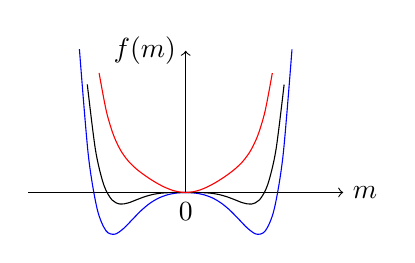
\begin{tikzpicture}
      \draw[->] (-2,0) -- (2,0) node[right] {$m$};
      \draw[->] (0,0) -- (0,1.8) node [left] {$f(m)$} ;
      \draw[domain=-1.35:1.35,smooth,variable=\x,blue] plot ({\x},{-0.5*\x*\x-\x*\x*\x*\x+\x*\x*\x*\x*\x*\x});
      \draw[domain=-1.25:1.25,smooth,variable=\x,black] plot ({\x},{-\x*\x*\x*\x+\x*\x*\x*\x*\x*\x});
      \draw[domain=-1.1:1.1,smooth,variable=\x,red] plot ({\x},{\x*\x-\x*\x*\x*\x+\x*\x*\x*\x*\x*\x});
      \draw (0,0) node[below]{0};
\end{tikzpicture}
\end{center}
\item Work with $x=m^2$, the free energy is
$$f(x)=\alpha x+\frac{1}{2}bx^2+\frac{1}{3}cx^3,\quad\alpha=a(T-T_c)$$
At the transition point, $T=T_c^*$, 
$$0=f(m=0)=f(m^*\neq 0)$$
to which the system jumps at $m^*$. So, find $f(x)=0$:
$$x=0,\text{ or } \alpha+\frac{1}{2}bx+\frac{1}{3}cx^2=0$$
which gives either $x=0\implies m=0$ or $(b/2)^2-4\alpha c/3=0\implies \alpha=\frac{3b^2}{16c}$. But, $\alpha=a(T-T_c)$, hence $T_c^*=T_c+\frac{3b^2}{16ac}$.
\item Our results have shown:
\begin{itemize}
    \item When $b>0$, there is a continuous phase transition from a disordered phase for $T>T_c$ to an ordered phase for $T<T_c$ (jump continuously from $m=0$ to $m\neq 0$). This phase transition boundary is a line along $b>0$ and $T=T_c$.
    \item When $b<0$, there is a discontinuous phase transition (jump discontinuously from 0 to $\sqrt{|b|/c}$). This phase transition boundary is a quadratic curve $T-T_c=\frac{3b^2}{16ac}$.
\end{itemize}
\begin{center}
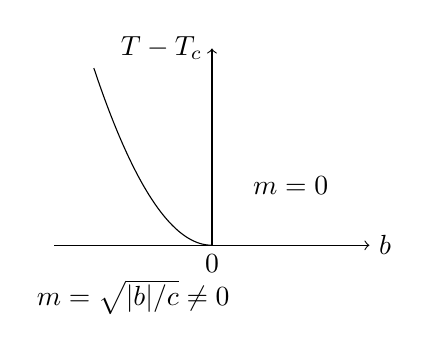
\begin{tikzpicture}
      \draw[->] (-2,0) -- (2,0) node[right] {$b$};
      \draw[->] (0,0) -- (0,2.5) node [left] {$T-T_c$} ;
      \draw[domain=-1.5:0,smooth,variable=\x,black] plot ({\x},{\x*\x});
      \draw (0,0) node[below]{0};
       \draw (1,1) node[below]{$m=0$};
       \draw (-1,-1) node[above]{$m=\sqrt{|b|/c}\neq 0$};
\end{tikzpicture}
\end{center}
\end{enumerate}
\end{ans}
\newpage
\subsubsection*{2020 Q3}
\begin{qns}
Consider a real scalar field $\phi(t, x)$ in 1 + 1 space-time dimensions, with action $S=\int\mathcal{L}dtdx$ and Lagrangian density
$$\mathcal{L}=\dot{\phi}^2-\gamma\phi'^2+\alpha\phi^2-\frac{\beta}{2}\phi^4$$
where $\dot{\phi}=\frac{\partial\phi}{\partial t}$ and $\phi'=\frac{\partial\phi}{\partial x}$, and $\alpha$, $\beta$, $\gamma$ are real and positive constants.
\begin{enumerate}[label=(\alph*)]
\item Find the units of $\alpha$, $\beta$ and $\gamma$, and use them to obtain a characteristic length scale and an energy scale for the system.\hfill\textbf{[7]}
\item Derive the components of the stress-energy tensor, and discuss its conservation. Use it to define the total energy E of the system.\hfill\textbf{[8]}
\item Consider a field that interfaces between the two constant values:
$$\lim_{x\rightarrow-\infty}\phi(x,t)=-\sqrt{\frac{\alpha}{\beta}},\quad \lim_{x\rightarrow+\infty}\phi(x,t)=\sqrt{\frac{\alpha}{\beta}}$$
Using an appropriate variational calculation ($\phi\rightarrow\phi+\delta\phi$), or otherwise, show that the field $\phi(x, t)$ which minimises the total energy $E$ for the above boundary conditions takes the form
$$\phi(x)=\sqrt{\frac{\alpha}{\beta}}\tanh\bigg[\sqrt{\frac{\alpha}{2\gamma}}(x-x_0)\bigg]$$
where $x_0$ is an arbitrary constant. (It is sufficient to show that $\delta E = 0$ and you do not need to demonstrate that it is an actual minimum.)\hfill\textbf{[10]}
%\item Define the energy $E_I$ of the interface as the difference between the energy of the field discussed in part (c), namely with the interface present, and the energy of a uniform field, $\phi=\sqrt{\alpha/\beta}$. Either by direct computation or by an appropriate scaling analysis, determine how EI depends on the parameters $\alpha$, $\beta$ and $\gamma$.\hfill\textbf{up to [5] bonus}
\end{enumerate}
\end{qns}
\begin{ans}\leavevmode
\begin{enumerate}[label=(\alph*)]
\item In natural units, $\hbar=1=c$, we have
$$c\sim LT^{-1}\implies [L]=[T],\quad\hbar\sim L^2MT^{-1}\implies[M]=[T]^{-1}=[L]^{-1}$$
Since the action $S=\int\mathcal{L}d^2x$ is dimensionless, we have $[S]=0$, $[d^2x]=[L]^{2}=[M]^{-2}$, and so $[\mathcal{L}]=[M]^2$. So the dimension of $\phi$ is
$$[\phi]=[\dot{\phi}][T]=\sqrt{[\mathcal{L}]}[T]=[M][T]=1$$
and hence $ [\alpha]=[M]^2=[\beta]$ and $[\phi']^2=[\phi]^2[L]^{-2}=[M]^2\implies[\gamma]=1$.
\item The stress-energy tensor is
$$T^{\mu\nu}=\frac{\partial\mathcal{L}}{\partial(\partial_\mu\phi)}\partial^\nu\phi-g^{\mu\nu}\mathcal{L},\quad g^{\mu\nu}=(-1)^\mu\delta_{\mu\nu}=(+1,-1,-1,-1)$$
Noting that $\partial^1\phi=-\partial_1\phi$, the components are
$$T^{00}=\frac{\partial\mathcal{L}}{\partial(\partial_0\phi)}\partial^0\phi-g^{00}\mathcal{L}=2\dot{\phi}^2-\dot{\phi}^2+\gamma\phi'^2-\alpha\phi^2+\frac{\beta}{2}\phi^4=\dot{\phi}^2+\gamma\phi'^2-\alpha\phi^2+\frac{\beta}{2}\phi^4$$
$$T^{01}=\frac{\partial\mathcal{L}}{\partial(\partial_0\phi)}\partial^1\phi-g^{01}\mathcal{L}=-2\dot{\phi}\phi',\quad T^{10}=\frac{\partial\mathcal{L}}{\partial(\partial_1\phi)}\partial^0\phi-g^{10}\mathcal{L}=-2\gamma\dot{\phi}\phi'$$
$$T^{11}=\frac{\partial\mathcal{L}}{\partial(\partial_1\phi)}\partial^1\phi-g^{11}\mathcal{L}=2\gamma\dot{\phi}^2+\dot{\phi}^2-\gamma\phi'^2+\alpha\phi^2-\frac{\beta}{2}\phi^4=\dot{\phi}^2+\gamma\phi'^2+\alpha\phi^2-\frac{\beta}{2}\phi^4$$
The energy is then $E=\int T^{00}dx=\int\dot{\phi}^2+\gamma\phi'^2-\alpha\phi^2+0.5\beta\phi^4dx$. The tensor is not symmetric unless $\gamma=1$. Further, $T^{00}=T^{11}$ only if $\alpha=\beta=0$. Since $\mathcal{L}$ is independent of the time coordinate and space coordinate, the stress-energy tensor is conserved, i.e. $\partial_\mu T^{\mu\nu}=0$.
\item We need to find $\phi(x,t)$ that minimizes the total energy $E$ of the system. Since the boundary conditions $\lim_{x\rightarrow\pm\infty}\phi(x)=\pm\sqrt{\alpha/\beta}$ is time-independent, the energy $E=\int(\gamma\phi'^2-\alpha\phi^2+0.5\beta\phi^4)dx$ is minimized when $\dot{\phi}=0$. Under the variations $\phi\rightarrow\phi+\delta\phi$, $\phi'\rightarrow\phi'+(\delta\phi)'$, the variation in energy is
$$\delta E=\int 2\gamma\phi'\delta\phi'-2\alpha\phi\delta\phi+2\beta\phi^3\delta\phi~dx$$
where $\phi'(\delta\phi)'=(\phi'\delta\phi)'-\phi''\delta\phi$ follows from integration by parts. But, the total derivative contributes a vanishing boundary term to the integral, hence we may drop this term.
$$\delta E=2\int[-\gamma\phi''-\alpha\phi+\beta\phi^3]\delta\phi~dx$$
$\delta E=0\implies\beta\phi^3=\gamma\phi''+\alpha\phi$ $\forall x$. We verify the given $\phi$ is a solution:
$$\gamma\phi''(x)=\gamma\sqrt{\frac{\alpha^2}{2\beta\gamma}}\frac{d}{dx}\frac{1}{\cosh^2[\sqrt{\frac{\alpha}{2\gamma}}(x-x_0)]}=-\alpha\frac{\phi}{\cosh^2[\sqrt{\frac{\alpha}{2\gamma}}(x-x_0)]}$$
$$-\alpha\phi(x)+\beta\phi(x)^3=-\alpha\phi(x)\bigg[1-\tanh^2\bigg[\sqrt{\frac{\alpha}{2\gamma}}(x-x_0)\bigg]\bigg]=\gamma\phi''(x)$$
and finally, the boundary condition is verified:
$$\lim_{x\rightarrow\pm\infty}\tanh\bigg[\sqrt{\frac{\alpha}{2\gamma}}(x-x_0)\bigg]=\pm1$$
The width of the interface $\sqrt{2\gamma/\alpha}$ is proportional to the characteristic length scale $\lambda=\sqrt{\gamma/\alpha}$.\\[5pt]
The solution is not unique due to the arbitrary choice of $x_0$, which is not fixed by the boundary conditions. This corresponds to the `centre' of the interface where $\phi(x)=0$. $x_0$ is arbitrary since both phases have exactly the same energy density, and the ratio of the space occupied by one or the other is not fixed by the minimization of energy.
%\item \textcolor{red}{?}
\end{enumerate}
\end{ans}
\newpage
\section{Propagators and Causality}
\subsection{Mathematics preliminaries}
\subsubsection{Dirac Delta functions and Green's functions}
\begin{defi}[Dirac delta function]
We have $\delta(x)=0$ whenever $x\neq 0$ and $\delta(x)$ to be not finite at $x=0$. Hence, we generalize $\delta(x-\xi)$ with the following properties
$$\delta(x-\xi)=0~\forall x\neq\xi,\quad\int_{-\infty}^\infty\delta(x-\xi)dx=1$$
This acts as a linear operator $\int\delta(x-\xi)dx$ on an arbitrary function $f(x)$ to produce a number $f(\xi)$, i.e.
$$\int_{-\infty}^\infty\delta(x-\xi)f(x)dx=f(\xi)$$
provided $f(x)$ is `well-behaved' at $x=\xi,\pm\infty$. In turn, we define the derivative of the Dirac delta:
$$\int_{-\infty}^\infty\delta'(x-\xi)f(x)dx=-f'(\xi)$$
\end{defi}
\begin{remarks}
$\delta(x)$ always appears inside an integral as a linear operator where it's well-defined. Physically, it represents a unit point source.
\end{remarks}
\begin{defi}[Heaviside function]
The unit step function aka the Heaviside function
$$
   \Theta(x)=
\left\{
        \begin{array}{ll}
      1 & x\geq0\\
      0 & x<0
        \end{array}
    \right.$$
    usually defined as 
$$\Theta(x)=\int_{-\infty}^x\delta(x')dx'$$
\end{defi}
\begin{thm}[Properties of Dirac delta function]\leavevmode
\begin{enumerate}
    \item Sampling property:
$$ \int_a^bf(x)\delta(x-\xi)dx
\left\{
        \begin{array}{ll}
      f(\xi) & a<\xi<b\\
      0 & \text{otherwise}
        \end{array}
    \right.$$
\item Even property: 
$$ \int_{-\infty}^\infty f(x)\delta(-(x-\xi))dx=\int_{-\infty}^\infty f(x)\delta(x-\xi)dx$$
\item Scaling property: 
$$\int_{-\infty}^\infty f(x)\delta(a(x-\xi))dx=\frac{1}{|a|}f(\xi)$$
\item Advanced scaling:
Suppose $g(x)$ has $n$ isolated zeros at $x_1,\dots,x_n$, then (with $g'(x_i)\neq 0$)
$$\delta(g(x))=\sum_{i=1}^n\frac{\delta(x-x_i)}{|g'(x_i)|}$$
\item Isolation property:
If $g(x)$ is continuous at $x=0$, then
$$g(x)\delta(x)=g(0)\delta(x)$$
\end{enumerate}
\end{thm}
\begin{prop}
The eigenfunction expansion of $\delta(x)$ is 
$$\delta(x)=\frac{1}{2L}\sum_{n=-\infty}^\infty e^{in\pi x/L}$$
\end{prop}
The general goal is to solve the inhomogeneous ODE
$$\mathcal{L}y=f(x)$$
on $a\leq x\leq b$ with $f$ bounded, subject to homogeneous b.c.s, say $y(a)=y(b)=0$. The Green's function $G(x,\xi)$ for the differential operator $\mathcal{L}$ is the solution for the unit point mass at $x=\xi$:
$$\mathcal{L}G(x,\xi)=\delta(x-\xi)$$
which satisfies homogeneous b.c.s $G(a,\xi)=G(b,\xi)=0$ or similar. By linearity, we can construct the solution by integrating over the source $f(x)$ with the Green's function
$$y(x)=\int_a^bG(x,\xi)f(\xi)d\xi$$
where $y$ satisfies the homogeneous b.c.s. One can check
$\mathcal{L}y=\int\mathcal{L}G(x,\xi)f(\xi)d\xi=\int\delta(x-\xi)f(\xi)d\xi=f(x)$, so the solution (3.23) is given by the inverse operator $\mathcal{L}^{-1}f$, where $\mathcal{L}^{-1}f=\int G(x,\xi)fd\xi$. Here, $G$ only depends on $\mathcal{L}$ and b.c.s, not $f$. The Green's function is split into two parts
$$ G(x,\xi)=
\left\{
        \begin{array}{ll}
      G_1(x,\xi) & a\leq x\leq\xi\\
      G_2(x,\xi) & \xi<x\leq b
        \end{array}
    \right.$$
and satisfies the following properties:
\begin{enumerate}
    \item homogeneous solution with homogeneous b.c.s: $G$ solves homogeneous equation $\forall x\neq\xi$, so
$$\mathcal{L}G_1=0,\quad\mathcal{L}G_2=0$$
    s.t. $G$ satisfies
$$ G_1(a,\xi)=0,\quad G_2(b,\xi)=0$$
    \item continuity condition: $G$ is continuous at $x=\xi$
$$ G_1(\xi,\xi)=G_2(\xi,\xi)$$
    \item jump condition: the derivative $G'(x,\xi)$ is discontinuous at $x=\xi$
$$[G']_{\xi_-}^{\xi_+}=\frac{dG_2}{dx}\bigg|_{x=\xi_+}-\frac{dG_1}{dx}\bigg|_{x=\xi_-}=\frac{1}{\alpha(\xi)}$$
\end{enumerate}
\begin{eg}[Boundary value problem]
Solve $y''=y=f(x)$, $y(0)=y(1)=0$ by constructing the $G(x,\xi)$. 
\begin{enumerate}
    \item homogeneous solution $y_1=e^x$, $y_2=e^{-x}$, so with homogeneous b.c.s (by inspection)
$$
  G(x,\xi)=\left\{
        \begin{array}{ll}
      C(\xi)\sinh x& 0\leq x<\xi\\
      D(\xi)\sinh(1-x) & \xi<x\leq 1
        \end{array}\right.$$
        \item continuous at $x=\xi$ gives  $    C\sinh\xi=D\sinh(1-\xi)\implies C=\frac{D\sinh(1-\xi)}{\sinh\xi}$
        \item discontinuous at $x=\xi$: $-D\cosh(1-\xi)-C\cosh\xi=1\implies -D\sinh(1)=\sinh\xi$, 
so the solution is
$$
y(x)=-\frac{\sinh(1-x)}{\sinh(1)}\int_0^x\sinh\xi f(\xi)d\xi-\frac{\sinh(x)}{\sinh(1)}\int_x^1\sinh(1-\xi)f(\xi)d\xi$$
\end{enumerate}
\end{eg}
\begin{remarks}[Inhomogeneous b.c.s]
Consider the modified problem: find $y_p$ solution to $\mathcal{L}y=0$ satisfying b.c.s $y(a)=c$ and $y(b)=d$.\\[5pt]
Then we try $y_g(x)=y(x)-y_p(x)$ s.t. $\mathcal{L}y_g=0$ with $y_g(a)=y_g(b)=0$. Consider $y''-y=f(x)$ but with b.c.s $y(0)=0$ and $y(1)=1$. The particular solution $y_p=A\sinh x+B\cosh x$ has the b.c.s $y_p(0)=0\implies B=0$ and $y_p(1)=1\implies A=\frac{1}{\sinh(1)}$. Now solve for $y_g=y-y_p$ with $y_g(0)=0$, $y_g(1)=0$ with solution $y(x)=\frac{\sinh x}{\sinh 1}+y_g(x)$.
\end{remarks}
\begin{remarks}[Higher order ODEs]
If $\mathcal{L}y=f(x)$ to $n$th order (coefficient $\alpha(x)$ for $y^{(n)}(x)$) with homogeneous b.c.s, then we generalize the Green's function to have the properties:
\begin{enumerate}
    \item $G_1$, $G_2$ are homogeneous solution satisfying homogeneous b.c.s;
    \item continuity $G_1=G_2$, $G_1'=G_2'$, $\dots$ $G_1^{(n-2)}=G_2^{(n-2)}$ at $x=\xi$;
    \item jump on $(n-1)$th derivative
    $$[G^{(n-1)}]_{\xi_-}^{\xi_+}=G_2^{(n-1)}|_{\xi_+}-G_1^{(n-1)}|_{\xi_-}=\frac{1}{\alpha(\xi)}$$
\end{enumerate}
\end{remarks}
\begin{eg}[Initial value problem]
Solve $y''-y=f(t)$ with $y(0)=y'(0)=0$.
\begin{enumerate}
    \item homogeneous solution and i.c.s: $t<\tau$, $G_1=0$ while $t>\tau$, $G_2=Ae^t+Be^{-t}$.
    \item continuity: $G(\tau,\tau)=0\implies G_2=D\sinh(t-\tau)$ for $t>\tau$.
    \item jump: $[G']=\frac{1}{\alpha}=1\implies G_2'(t,\tau)=D\cosh 0=D=1$.
\end{enumerate}
The solution is $y(t)=\int_0^tf(\tau)\sinh(t-\tau)d\tau$
\end{eg}
\begin{remarks}
Causality is `built-in' as only forces acting prior to $t$ affect the solution at $t$.
\end{remarks}
\subsubsection{Fourier Transform}
\begin{defi}[Fourier transform]
The Fourier transform of a function $f(x)$ is
$$\tilde{f}(k):=\mathcal{F}[f(x)]=\int_{-\infty}^\infty f(x)e^{-ikx}dx$$
and the inverse Fourier transform is
$$f(x)=\mathcal{F}^{-1}[\tilde{f}(k)]=\frac{1}{2\pi}\int_{-\infty}^\infty\tilde{f}(k)e^{ikx}dk$$
\end{defi}
Beware there are several conventions.
\begin{thm}[Fourier inversion theorem]
For the following to be true
$$\mathcal{F}^{-1}[\mathcal{F}[f(x)]]=f(x)$$
it is sufficient to require $f$ and $\tilde{f}$ to be absolutely integrable, i.e. $\int_{-\infty}^\infty|f(x)|dx=M<\infty$, so $f\rightarrow 0$ as $x\rightarrow\pm\infty$.
\end{thm}
From here onwards, we assume all functions mentioned will have a Fourier transform.
\begin{thm}[Properties of Fourier transform]\leavevmode
\begin{enumerate}
    \item linearity: 
$$h(x)=\lambda f(x)+\mu g(x)\iff\tilde{h}(k)=\lambda\tilde{f}(k)+\mu\tilde{g}(k)$$
    \item translation and re-phasing:
$$ h(x)=f(x-\lambda)\iff\tilde{h}(k)=e^{-i\lambda k}\tilde{f}(k)$$
$$h(x)=e^{i\lambda x}f(x)\iff\tilde{h}(k)=\tilde{f}(k-\lambda)$$
    \item scaling:
$$h(x)=f(\lambda x)\iff\tilde{h}(k)=\frac{1}{|\lambda|}\tilde{f}(k/\lambda)$$
    \item derivative:
$$h(x)=xf(x)\iff\tilde{h}(k)=i\tilde{f}'(k)$$
$$h(x)=f'(x)\iff\tilde{h}(k)=ik\tilde{f}(k)$$
    \item duality:
$$g(x)=\tilde{f}(x)\iff\tilde{g}(k)=2\pi f(-k)$$
\end{enumerate}
\end{thm}
\begin{eg}[Top-hat]
Consider top-hat function $f(x)=1$ for $|x|\leq a$ (where $a>0$) and $f(x)=0$ for $|x|>a$. The Fourier transform is
$$\tilde{f}(k)=\int_{-\infty}^\infty f(x)e^{ikx}dx=\int_{-a}^a\cos(kx)dx=\frac{2\sin(ka)}{k}$$
Fourier inversion theorem gives
$$   \frac{1}{2\pi}\int_{-\infty}^\infty e^{ikx}\frac{2\sin ka}{k}dk=
\left\{
        \begin{array}{ll}
      1 & |x|\leq a\\
      0 & |x|>a
        \end{array}
    \right.$$
Set $x=0$, then take $k\rightarrow x$ to get the Dirichlet's discontinuity formula:
$$\int_{-\infty}^\infty\frac{\sin(ax)}{x}dx=\left\{
        \begin{array}{ll}
      \pi/2 & a>0\\
      0 & a=0\\
      -\pi/2 & a<0
        \end{array}
    \right.=\frac{\pi}{2}\sgn(a)$$
\end{eg}
\begin{thm}[Convolution theorem]
$$\tilde{h}(k)=\tilde{f}(k)\tilde{g}(k)\iff h(x)=(f*g)(x):=\int_{-\infty}^\infty f(y)g(x-y)dy$$
$$h(x)=f(x)g(x)\iff\tilde{h}(k)=\frac{1}{2\pi}(\tilde{f}*\tilde{g})(k):=\frac{1}{2\pi}\int_{-\infty}^\infty\tilde{f}(p)\tilde{g}(k-p)dp$$
\end{thm}
\begin{prop} Fourier transform preserves the inner product between two functions, i.e.
$$\langle g,f\rangle=\int_{-\infty}^\infty f(x)g^*(x)dx=\frac{1}{2\pi}\int_{-\infty}^\infty\tilde{f}(k)\tilde{g}^*(k)dk=\frac{1}{2\pi}\langle\tilde{g},\tilde{f}\rangle$$
\end{prop}
\begin{cor}[Parseval's theorem]
$$\int_{-\infty}^\infty|f(x)|^2dx=\frac{1}{2\pi}\int_{-\infty}^\infty|\tilde{f}(k)|^2dk$$
\end{cor}
\begin{prop}\leavevmode
\begin{enumerate}
    \item 
$$\mathcal{F}[\delta(x)]=1\iff\mathcal{F}[1]=2\pi\delta(k)$$
    \item
$$\mathcal{F}[\delta(x-a)]=e^{-ika}$$
\end{enumerate}
\end{prop}
\begin{cor}
$$f(x)=\cos\omega x\iff\tilde{f}(k)=\pi(\delta(k+\omega)+\delta(k-\omega))$$
$$f(x)=\sin\omega x\iff\tilde{f}(k)=\pi(\delta(k+\omega)-\delta(k-\omega))$$
\end{cor}
\begin{eg}[Damped oscillator]
Solve $\mathcal{L}y=y''+2py'+(p^2+q^2)y=f(t)$ with damping $p>0$ and homogeneous b.c.s $y(0)=y'(0)=0$. The Fourier transform is
$$(i\omega)^2\tilde{y}+2ip\omega\tilde{y}+(p^2+q^2)\tilde{y}=\tilde{f}\implies\tilde{y}=\frac{\tilde{f}}{-\omega^2+2ip\omega+p^2+q^2}:=\tilde{R}(\omega)\tilde{f}(\omega)$$
Inverting with Convolution theorem (4.17),
$$y(t)=\int_0^tR(t-\tau)f(\tau)dt,\quad R(t-\tau)=\frac{1}{2\pi}\int_{-\infty}^\infty\frac{e^{i\omega(t-\tau)}d\omega}{p^2+q^2+2ip\omega-\omega^2}$$
One can show $\mathcal{L}R(t-\tau)=\delta(t-\tau)$, i.e. the response function $R(t-\tau)$ is the Green's function.
\end{eg}
\newpage
\subsubsection{Complex methods}
\begin{defi}[Analytic]
We say $f$ is analytic at $z$ if $\exists$ a neighbourhood of $z$ throughout which $f'$ exists.
\end{defi}
\begin{defi}[Singularity]
A singularity of $f$ is a point at which it is not analytic, or not even defined.
\end{defi}
If $f$ might have a singularity at $z_0$, then we cannot necessarily expect it to have a Taylor series there.
\begin{defi}[Laurent series]
If $f$ is analytic in an annulus $R_1<|z-z_0|<R_2$, then it has a Laurent series about $z_0$, of the form
$$f(z)=\sum_{n=-\infty}^\infty a_n(z-z_0)^n$$
which is convergent within the annulus.
\end{defi}
\begin{defi}[Pole]
If $f$ has a pole at $z_0$, then $\lim_{z\rightarrow z_0}|f(z)|=\infty$.
\end{defi}
\begin{remarks}
Consider the Laurent series $\sum_{n=-\infty}^\infty a_n(z-z_0)^n$, then if $\exists N>0$ s.t. $a_n=0$ $\forall n<-N$, but $a_{-N}\neq 0$, then $f$ has a pole of order $N$ at $z_0$ (simple pole at $N=1$, double pole at $N=2$, etc).
\end{remarks}
\begin{defi}[Residue]
The residue of $f$ at $z_0$ is the coefficient of $a_{-1}$ of its Laurent series.
\end{defi}
\begin{notation}
We denote the residue as $\res_{z=z_0}f(z)$.
\end{notation}
\begin{prop}\leavevmode
\begin{enumerate}
    \item At a simple pole, the residue is $\res_{z=z_0}f(z)=\lim_{z\rightarrow z_0}((z-z_0)f(z))$.
    \item More generally, at a pole of order $N$, the residue is $$\res_{z=z_0}f(z)=\lim_{z\rightarrow z_0}\bigg[\frac{1}{(N-1)!}\frac{d^{N-1}}{dz^{N-1}}((z-z_0)^Nf(z)\bigg]$$
\end{enumerate}
\end{prop}
\begin{thm}[Residue theorem]
Suppose $f$ is analytic in a simply-connected domain except at a finite number of isolated singularities $\{z_1,\dots,z_n\}$. Suppose a simple closed contour $\gamma$ encircles the origin anticlockwise, then
$$\oint_\gamma f(z)dz=2\pi i\sum_{k=1}^n\res_{z=z_k}f(z)$$
\begin{center}
  \begin{tikzpicture}
    \draw [->-=0.3, ->-=0.7, ->-=0.9] plot [smooth cycle] coordinates {(-2.4, -1.3) (0, -1.3) (1.4, -2) (2.6, -1.7) (2.8, 0.6) (0.6, 1.9) (-3.4, 0.8)};
    \node [circle] (z1) at (1.8, 0) {$\times$};
    \node [right] at (z1) {$z_1$};
    \node [circle] (z2) at (0, 1) {$\times$};
    \node [right] at (z2) {$z_2$};
    \node [circle] (z3) at (-2, -0.5) {$\times$};
    \node [right] at (z3) {$z_3$};
    \node at (3, 1) {$\gamma$};
  \end{tikzpicture}
\end{center}
\end{thm}
\begin{eg}
Evaluate
$$I=\int_0^\infty\frac{dx}{1+x^2}$$
Consider $\oint_\gamma\frac{dz}{1+z^2}$, where $\gamma$ is the contour consisting of $\gamma_0$ followed by $\gamma_R$: from $-R$ to $R$ along the real axis, then returning to $-R$ via a semicircle of radius $R$ in the upper half plane. This is known as \textbf{closing in the upper half-plane} or closing above.
\begin{center}
    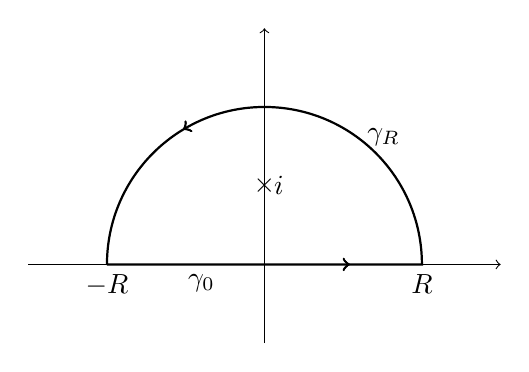
\begin{tikzpicture}
      \draw [->] (-3, 0) -- (3, 0);
      \draw [->] (0, -1) -- (0, 3);

      \draw [black, thick, ->-=0.3, ->-=0.8] (-2, 0) -- (2, 0) node [pos=0.3, below] {$\gamma_0$} arc(0:180:2) node [pos=0.3, right] {$\gamma_R$};

      \node [below] at (-2, 0) {$-R$};
      \node [below] at (2, 0) {$R$};

      \node at (0, 1) {$\times$};
      \node [right] at (0, 1) {$i$};
    \end{tikzpicture}
  \end{center}
Now $\frac{1}{1+z^2}=\frac{1}{(z+i)(z-i)}$, so the only singularity enclosed by $\gamma$ is a simple pole at $z=i$, whose residue is $\lim_{z\rightarrow i}\frac{z-i}{z^2+1}=\frac{1}{2i}$. Hence,
$$\oint_{\gamma_0}\frac{dz}{1+z^2}+\oint_{\gamma_R}\frac{dz}{1+z^2}=\oint_{\gamma}\frac{dz}{1+z^2}=2\pi i\res_{z=i}\frac{1}{1+z^2}=\pi$$
But 
$$\oint_{\gamma_0}\frac{dz}{1+z^2}=\int{-R}^R\frac{dx}{1+x^2}\rightarrow 2I,\text{  as  }R\rightarrow\infty$$
Also, we can justify $\int_{\gamma_R}\frac{dz}{1+z^2}\rightarrow 0$ as $R\rightarrow\infty$. Doing this informally: for $z\in\gamma_R$, we use the ML inequality:
$$\bigg|\frac{1}{1+z^2}\bigg|=O(R^{-2})\implies\bigg|\int_{\gamma_R}\frac{dz}{1+z^2}\bigg|\leq\pi R~O(R^{-2})=O(R^{-1})\rightarrow 0,\text{ as }R\rightarrow\infty$$
as we will see later, the informal argument is easier for more difficult integrals.
\end{eg}
\begin{eg}
For $I=\int_0^\infty\frac{dx}{1+x^4}$, use the same contour $\gamma$ again. There are simple poles at $e^{\pm i\pi/4}$, $e^{\pm 3\pi i/4}$, but only the first two are enclosed, with residues $-\frac{1}{4}e^{i\pi/4}$ and $+\frac{1}{4}e^{-i\pi/4}$. The integral round the semicircle is bounded by $\pi R~O(R^{-4})\rightarrow 0$ as $R\rightarrow\infty$. Hence,
    $$2I=2\pi i(-0.25e^{\pi i/4}+0.25e^{-\pi i/4})\implies I=\frac{\pi}{2\sqrt{2}}$$
    Alternatively could use a quarter circle contour to enclose one pole only, say $e^{i\pi/4}$.
\end{eg}
\begin{eg}
Evaluate
$$I=\int_0^{2\pi}\frac{d\theta}{a+\cos\theta},\quad a>1$$
so that the integrand is always finite. Substitute $z=e^{i\theta}$,
$$I=\oint_{\gamma}\frac{(iz)^{-1}dz}{a+0.5(z+z^{-1})}=-2i\oint_\gamma\frac{dz}{z^2+2az+1}$$
where the integrand has poles $z_\pm=-a\pm\sqrt{a^2-1}$, both on the real axis. Since $a-1<\sqrt{a^2-1}<a$, then $-1<z_+<0$, i.e. $z_+$ is inside the unit circle. 
 \begin{center}
    \begin{tikzpicture}
      \draw [->] (-3, 0) -- (3, 0);
      \draw [->] (0, -3) -- (0, 3);
      \draw [black, thick, ->-=0.2,->-=0.7] circle [radius=1.8];
      \node [right] at (1.2726, 1.2726) {$\gamma$};

      \node (z-) at (-2.5, 0) {$\times$};
      \node [below] at (z-) {$z_-$};

      \node (z+) at (-1.2, 0) {$\times$};
      \node [below] at (z+) {$z_+$};
    \end{tikzpicture}
  \end{center}

The residue at $z=z_+$ is
$$\res_{z=z_+}\frac{1}{z^2+2az+1}=\lim_{z\rightarrow z_+}\frac{z-z_+}{z^2+2az+1}=\frac{1}{z_+-z_-}=\frac{1}{2\sqrt{a^2-1}}$$
Hence, $I=-2i\frac{2\pi i}{2\sqrt{a^2-1}}=\frac{2\pi}{\sqrt{a^2-1}}$.
\end{eg}
\begin{lemma}[Jordan's Lemma]
Suppose $f$ is analytic function, except for a finite number of singularities, and $f(z)\rightarrow 0$ as $|z|\rightarrow\infty$. Then for any real constant $\lambda>0$,
$$\int_{\gamma_R}f(z)e^{i\lambda z}dz\rightarrow 0,~\text{ as }R\rightarrow\infty$$
where $\gamma_R$ is a semicircle of radius $R$ in the upper half-plane. For $\lambda<0$, same conclusion holds for semicircle $\gamma_R$ in the lower half-plane.
\begin{center}
    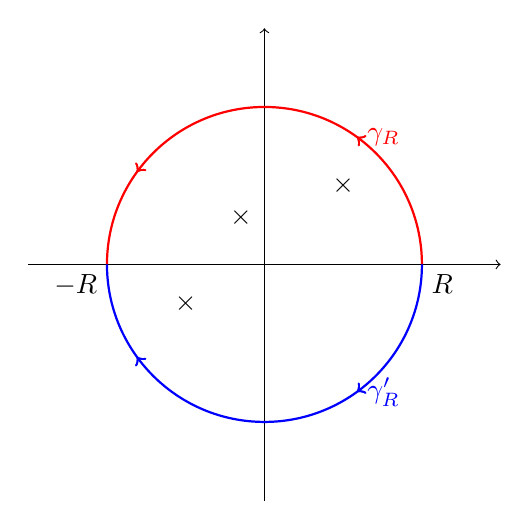
\begin{tikzpicture}
      \draw [->] (-3, 0) -- (3, 0);
      \draw [->] (0, -3) -- (0, 3);

      \draw [red, thick, ->-=0.3, ->-=0.8] (2, 0) arc(0:180:2) node [pos=0.3, right] {$\gamma_R$};
      \draw [blue, thick, ->-=0.3, ->-=0.8] (2, 0) arc(0:-180:2) node [pos=0.3, right] {$\gamma_R'$};

      \node [anchor = north east] at (-2, 0) {$-R$};
      \node [anchor = north west] at (2, 0) {$R$};
      \node [circle] at (-2, 0) {};
      \node [circle] at (2, 0) {};

      \node at (1, 1) {$\times$};
      \node at (-1, -0.5) {$\times$};
      \node at (-0.3, 0.6) {$\times$};
    \end{tikzpicture}
  \end{center}
\end{lemma}
\begin{eg}[Using contour integration to invert Fourier transforms]
Consider $f(x)=e^{-\alpha x}H(x)$, where $a>0$ is a real constant. Then,
$$\tilde{f}(k)=\int_0^\infty e^{-ax-ikx}dx=-\frac{1}{a+ik}[e^{-ax-ikx}]_0^\infty=\frac{1}{a+ik}$$
Verify this result by evaluating $\frac{1}{2\pi}\int_{-\infty}^\infty\tilde{f}(k)e^{ikx}dk$. In complex $k$-plane, let $\gamma_0$ be contour from $-R$ to $R$ on real axis, $\gamma_R$ be semicircle of radius $R$ in the upper half-plane, $\gamma_R'$ be semicircle of radius $R$ in the lower half-plane. Let $\gamma$ be $\gamma_0$ followed by $\gamma_R$, and let $\gamma'$ be $\gamma_0$ followed by $\gamma_R'$.
\begin{center}
    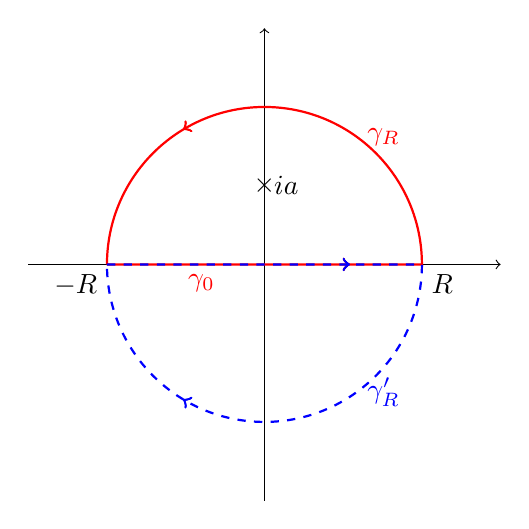
\begin{tikzpicture}
      \draw [->] (-3, 0) -- (3, 0);
      \draw [->] (0, -3) -- (0, 3);

      \draw [red, thick, ->-=0.3, ->-=0.8] (-2, 0) -- (2, 0) node [pos=0.3, below] {$\gamma_0$} arc(0:180:2) node [pos=0.3, right] {$\gamma_R$};
      \draw [dashed, blue, thick, ->-=0.3, ->-=0.8] (-2, 0) -- (2, 0) arc(0:-180:2) node [pos=0.3, right] {$\gamma_R'$};

      \node [anchor = north east] at (-2, 0) {$-R$};
      \node [anchor = north west] at (2, 0) {$R$};

      \node at (0, 1) {$\times$};
      \node [right] at (0, 1) {$ia$};
    \end{tikzpicture}
  \end{center}
Now $\tilde{f}(k)$ has only one pole, $k=ia$. This pole is simple.
$$\oint_\gamma\tilde{f}(k)e^{ikx}dk=2\pi i\res_{k=ia}\frac{e^{ikx}}{i(k-ia)}=2\pi e^{-ax}$$
$$\oint_{\gamma'}\tilde{f}(k)e^{ikx}dk=-0$$
Now if $x>0$, we can apply the Jordan's Lemma with $\lambda =x$, to $\gamma_R$ to show that $\int_{\gamma_R}\tilde{f}(k)e^{ikx}dk\rightarrow 0$ as $R\rightarrow\infty$ since $\tilde{f}(k)=O(1/k)$ as $|k|\rightarrow\infty$. Hence for $x>0$,
$$\frac{1}{2\pi}\int_{-\infty}^\infty\tilde{f}(k)e^{ikx}dk=\frac{1}{2\pi}\lim_{R\rightarrow\infty}\oint_\gamma\tilde{f}(k)e^{ikx}dk=e^{-ax}$$
For $x<0$, close the lower half-plane instead and use $\gamma'$:
$$\frac{1}{2\pi}\int_{-\infty}^\infty\tilde{f}(k)e^{ikx}dk=\frac{1}{2\pi}\lim_{R\rightarrow\infty}\oint_{\gamma'}\tilde{f}(k)e^{ikx}dk=0$$
\end{eg}
\begin{remarks}[Indentation Lemma]
Whenever there is a singular point on the real axis, we will have to consider an indentation contour.
 \begin{center}
    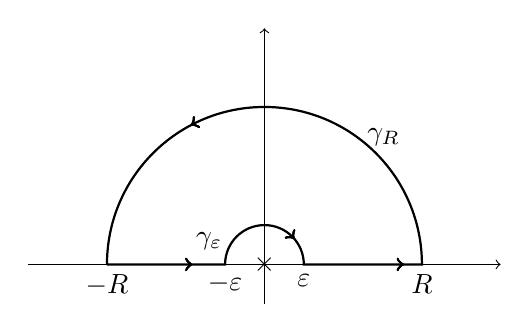
\begin{tikzpicture}
      \draw [->] (-3, 0) -- (3, 0);
      \draw [->] (0, -0.5) -- (0, 3);
      \draw [black, thick, ->-=0.1, ->-=0.25, ->-=0.4, ->-=0.8] (-2, 0) node [below] {$-R$} -- (-0.5, 0) node [below] {$-\varepsilon$} arc(180:0:0.5) node [pos=0.2, left] {$\gamma_\varepsilon$} node [below] {$\varepsilon$} -- (2, 0) node [below] {$R$} arc(0:180:2) node [pos=0.3, right] {$\gamma_R$};

      \node {$\times$};
    \end{tikzpicture}
  \end{center}
In general, if $\gamma_\varepsilon$ is an anti-clockwise arc of radius $\varepsilon$ and angle $\alpha$ centred around a simple pole $z_0$ of function $f(z)$, then 
$$\int_{\gamma_\varepsilon}f(z)dz\rightarrow i\alpha\res_{z=z_0}f(z),\text{ as }\varepsilon\rightarrow0$$
i.e. a fraction $\frac{\alpha}{2\pi}$ of the value of the integral around an entire cycle.
\end{remarks}
\begin{defi}[Cauchy's Principal Value]
If $f(z)$ is "badly" behaved at $x=c$ and $a<c<b$, we define the Cauchy Principal Value (CPV) integral by 
$$\mathcal{P}\int_{a}^{b}dx:=\lim_{\epsilon\rightarrow0}\bigg[\int_{a}^{c-\epsilon}f(x)dx+\int_{c+\epsilon}^{b}f(x)dx\bigg]$$
if the limit exist. For the Cauchy Princial Value at infinity we define
$$\mathcal{P}\int_{-\infty}^{\infty}f(x)dx=\lim _{R\rightarrow\infty}\int_{-R}^{R}f(x)dx$$
if the limit exists.
\end{defi}
\begin{eg}
Define $I=\mathcal{P}\int_{-\infty}^{\infty	}\frac{f(x)}{x}dx$, where $f(z)$ is  analytic in the upper half-plane (include real axis) and $|f(z)|\rightarrow0$ as $|z|\rightarrow \infty$. This only make sense as a Cauchy Principal Value.
\end{eg}
\newpage
\subsection{Physical Examples}
\begin{eg}[Damped harmonic oscillator]
The amplitude of a driven damped harmonic oscillator satisfy
$$\ddot{x}(t)+2\gamma\dot{x}(t)+\omega_0^2x(t)=f(t)$$
where $f(t)$ is the forcing function, $\omega_0>0$ is real and $\gamma>0$ is real and represents the effects of damping. Assume $x(t)\rightarrow0$ as $|t|\rightarrow\infty$ so that we can define the Fourier transform of $x(t)$. After Fourier transforming the PDE we arrive at
$$\tilde{x}(\omega)=-\frac{\tilde{f}(\omega)}{(\omega-\omega_+)(\omega-\omega_-)}:=\tilde{f}(\omega)\tilde{g}(\omega)$$
where $\omega_\pm=i\gamma\pm\sqrt{\omega_0^2-\gamma^2}$. Find $x(t)$ by taking inverse Fourier transform and invoke convolution theorem:
$$x(t)=\int_{-\infty}^\infty f(s)g(t-s)dt,\quad g(\tau)=\frac{1}{2\pi}\int_{-\infty}^\infty\frac{-e^{i\omega\tau}d\omega}{(\omega-\omega_+)(\omega-\omega_-)}$$
This is equivalent to a solution using the Green function $G(t,s)=g(t-s)$ of $\mathcal{L}=\frac{d^2}{dt^2}+2\gamma\frac{d}{dt}+\omega_0^2$. Use contour integration to evaluate. If $\tau<0$, close the lower half-plane (invoke Jordan's Lemma) and if $\tau>0$, close the upper half-plane (invoke Jordan's Lemma). There are two poles enclosed in $\tau>0$, so $g(\tau>0)=\frac{1}{2\pi}\oint_C\tilde{g}(\omega)e^{i\omega\tau}d\omega$ where $C$ is the semi-circle in the upper-half plane. But there are no poles enclosed in $\tau<0$, so $g(\tau<0)=0\implies x(t<0)=0$. This is consistent with causal behaviour. Evaluating the residues, we then use residue theorem to show for the different regimes of damping:
$$g(\tau>0)=
\left\{
        \begin{array}{ll}
      \frac{e^{-\gamma\tau}}{\sqrt{\omega_0^2-\gamma^2}}\sin(\tau\sqrt{\omega_0^2-\gamma^2}) & \gamma<\omega_0\\
      \frac{e^{-\gamma\tau}}{\sqrt{-\omega_0^2+\gamma^2}}\sinh(\tau\sqrt{-\omega_0^2+\gamma^2}) & \gamma>\omega_0\\
      \tau e^{-\gamma\tau} & \gamma=\omega_0
        \end{array}
    \right.$$
\end{eg}
\begin{eg}[Free particle]
Consider the following equation:
$$i\hbar\frac{\partial\psi}{\partial t}+\frac{\hbar^2}{2m}\nabla^2\psi=F(x,t)$$
The corresponding Green's function $G$ satisfies
$$\bigg(i\hbar\frac{\partial}{\partial t}+\frac{\hbar^2}{2m}\nabla^2\bigg)G(x,x';t,t)=\delta(x-x')\delta(t-t')$$
We solve this by performing Fourier transform to reciprocal space and then to frequency space, i.e.
\begin{eqnarray}
\int_{-\infty}^\infty e^{ip(x-x')/\hbar}\delta(x-x')dx'\delta(t-t')&=&\int_{-\infty}^\infty\bigg(i\hbar\frac{\partial}{\partial t}+\frac{\hbar^2}{2m}\nabla^2\bigg)G(x,x';t,t')e^{ip(x-x')/\hbar}dx'\nonumber\\\delta(t-t')&=&\bigg(i\hbar\frac{\partial}{\partial t}-\frac{p^2}{2m}\bigg)G(p;t,t')\nonumber\\\int_{-\infty}^\infty e^{iE(t-t')/\hbar}\delta(t-t')dt'&=&\int_{-\infty}^\infty\bigg(i\hbar\frac{\partial}{\partial t}-\frac{p^2}{2m}\bigg)G(p;t,t')e^{iE(t-t')/\hbar}dt'\nonumber\\1&=&\bigg(E-\frac{p^2}{2m}\bigg)G(p;E)\nonumber
\end{eqnarray}
The Green's function is $G(p;t,t')=\frac{1}{2\pi}\int e^{-iE(t-t')/\hbar}\frac{1}{E-p^2/2m}\frac{dE}{\hbar}$, which we will solve using contour integration. There is a first-order pole on the real axis $E=p^2/2m$. Translate the pole $E\rightarrow E-i\varepsilon$ to the lower half-plane, so as to impose causality. The causality condition is $G(p;t<t')=0$ (no response in the absence of $F$ which is only present after $t>t'$). When $t-t'<0$, $-E(t-t')>0$ only if $E>0$, so by Jordan's Lemma and Cauchy's residue theorem, we must have no poles enclosed when we close the upper half-plane, so $G(p;t<t')=0$. Using Cauchy's residue theorem,
$$G(p;t>t')=\lim_{\varepsilon\rightarrow 0}\frac{1}{2\pi}\int_{-\infty}^\infty\frac{e^{-iE(t-t')/\hbar}}{E-i\varepsilon-p^2/2m}\frac{dE}{\hbar}=-\frac{2\pi i}{2\pi\hbar}e^{-i\frac{p^2}{2m\hbar}(t-t')}$$
where we incur a minus sign since the semi-circular contour traverses clockwise in the lower half-plane. To solve for the wavefunction, we must compute
$$\psi(x,t)=\int_{t>t'}\int G(x,x';t,t')F(x',t')dx'dt'=\int\int\int G(p;t>t')e^{-ip(x-x')/\hbar}dpdx'dt$$
\end{eg}
\begin{remarks}
For relativistic quantum mechanics, the Green's function is instead
$$G(p;E)=\frac{1}{E^2-p^2c^2-m^2c^4-i\varepsilon},\quad\varepsilon>0$$
which has two poles $E=\pm\sqrt{p^2c^2+m^2c^4+i\varepsilon}$ in each half-plane of complex $E$-space. This does not violate causality, as the answer corresponds to particles and anti-particles. Generally, relativistic systems have time-reversal symmetry.
\end{remarks}
\subsection{Kramers-Kronig Relations}
\begin{eg}[Linear response]
A dynamical variable $u(t)$ with zero average, $\langle u\rangle = 0$, always has a conjugate force $f(t)$ defined so that the corresponding perturbation of the potential energy is $−uf$. For a time varying force, its response is
$$\langle u(t)\rangle_f=\int_{-\infty}^\infty\alpha(t-t')f(t')dt'\iff\langle u(\omega)\rangle_f=\alpha(\omega)f(\omega)$$
where $\alpha$ is a generalized susceptibility, called a linear response function.
\end{eg}
\begin{prop}
Causality demands that $\alpha(t-t')$ is finite only for $t>t'$ and is zero for $t<t'$. This imposes constraints on $\text{Re}[\alpha]$ and $\text{Im}[\alpha]$, which becomes dependent on each other via the Kramers-Kronig relations:
$$\text{Re}[\alpha(\omega)]=\mathcal{P}\int\frac{\text{Im}[\alpha(\omega)]}{\omega'-\omega}\frac{d\omega'}{\pi},\quad\text{Im}[\alpha(\omega)]=-\mathcal{P}\int\frac{\text{Re}[\alpha(\omega')]}{\omega'-\omega}\frac{d\omega'}{\pi}$$
\end{prop}
\begin{proof}
Causality condition is $\alpha(t)=\Theta(t)v(t)$. By convolution theorem:
$$\alpha(\omega)=\int_{-\infty}^\infty\Theta(\omega-\omega_1)v(\omega_1)\frac{d\omega_1}{2\pi}$$
But, the Fourier transform of a step function is
$$\Theta(\omega)=\int_{-\infty}^\infty\Theta(t)e^{i\omega t}dt=\bigg[\int_0^\infty e^{i\omega t-\varepsilon t}dt\bigg]\bigg|_{\varepsilon\rightarrow 0}=\frac{1}{\varepsilon-i\omega}\bigg|_{\varepsilon\rightarrow 0}=\lim_{\varepsilon\rightarrow 0}\bigg[\frac{\varepsilon}{\omega^2+\varepsilon^2}+\frac{i\omega}{\omega^2+\varepsilon^2}\bigg]=\pi\delta(\omega)+\mathcal{P}\frac{i}{\omega}$$
We thus have the response function to be
$$\alpha(\omega)=\int_{-\infty}^\infty\bigg[\pi\delta(\omega-\omega_1)+\mathcal{P}\frac{i}{\omega-\omega_1}\bigg]v(\omega_1)\frac{d\omega_1}{2\pi}=\frac{1}{2}v(\omega')+\mathcal{P}\int\frac{i}{\omega}v(\omega-\omega')\frac{d\omega'}{2\pi}$$
To obtain the two relations, consider separately:
\begin{itemize}
    \item Assume $v(t)$ to be anti-symmetric, then $v(\omega)$ is purely imaginary. Then, we have $i\text{Im}[\alpha]=0.5v(\omega)$. Hence,
    $$\alpha(\omega)=i\text{Im}[\alpha(\omega)]-\mathcal{P}\int\frac{2\text{Im}[\alpha(\omega)]}{\omega-\omega'}\frac{d\omega'}{2\pi}\implies\text{Re}[\alpha(\omega)]=\mathcal{P}\int\frac{\text{Im}[\alpha(\omega)]}{\omega'-\omega}\frac{d\omega'}{\pi}$$
    \item Assume $v(t)$ to be symmetric, then $v(\omega)$ is purely real. Then, we have $\text{Re}[\alpha]=0.5v(\omega)$. Hence,
    $$\alpha(\omega)=i\text{Re}[\alpha(\omega)]+\mathcal{P}\int\frac{i2\text{Re}[\alpha(\omega)]}{\omega-\omega'}\frac{d\omega'}{2\pi}\implies\text{Im}[\alpha(\omega)]=-\mathcal{P}\int\frac{\text{Re}[\alpha(\omega)]}{\omega'-\omega}\frac{d\omega'}{\pi}$$
\end{itemize}
\end{proof}
\begin{remarks}
An important identity: Fourier transform of step function:
$$\Theta(\omega)=\pi\delta(\omega)+\mathcal{P}\frac{i}{\omega}$$
\end{remarks}
A more general proof, using Cauchy integration, is as follow:
\begin{thm}[Kramers-Kronig relations]
Let $f=u+iv$ be analytic in $\text{Im}[z]>0$, with $f\rightarrow0$ as $|z|\rightarrow\infty $. Then, 
$$\mathcal{P}\int_{-\infty}^{\infty}\frac{u(x)}{x-x'}dx=-\pi v(x'),\quad\mathcal{P}\int_{-\infty}^{\infty}\frac{v(x)}{x-x'}dx=\pi u(x')$$
\end{thm}
\begin{proof}
Consider $\oint_C\frac{f(z)}{z-z'}dz$. Let $x'=z'\in\mathbb{R}$ (along real axis), and consider an indentation contour around this singularity. Then, by the indentation lemma,
\begin{align*}
\oint_{C}\frac{f(z)}{z-z'}dz=\mathcal{ P}\int_{-\infty}^{\infty}\frac{f(x)}{x-x'}dx-i\pi f(x')=0\tag{*}
\end{align*}
For $z\in\mathbb{R}$, we can write $f(z)=f(x,y)=f(x,0)$, with 
$$f(x,0)=u(x,0)+iv(x,0)\implies\quad f(x)=u(x)+iv(x)$$
The Kramers' Kronig relations follow by taking the real and imaginary parts of (*).
\end{proof}
\begin{eg}
Let $u(x,y)$ be a function that satisfies $\nabla^2u=0$ in the upper half-plane, then $\frac{\partial u}{\partial x}$ and $\frac{\partial u}{\partial y}$ satisfy the Kramers-Kronig relations.
\end{eg}
\begin{eg}[Response function for atomic polarizability]
In electrostatics, the frequency dependence in the permittivity $\varepsilon(\omega)$ induces a non-locality between $\mathbf{D}$ and $\mathbf{E}$. Consider the simple atomic model, where $\varepsilon_r(\omega)-1$ has simple poles at $\omega_\pm=\pm(\omega_0^2-\gamma^2/4)^{1/2}-i\gamma/2$
$$\varepsilon_r(\omega)-1=\frac{nq^2}{m\varepsilon_0(\omega_0^2-\omega^2-i\gamma\omega)}$$
We evaluate the response function by closing the contour in the lower half-plane (where the two poles are at) for $t>0$, and thus obtain
$$G(t)=-\frac{nq^2}{m\varepsilon_0}\int_{-\infty}^\infty\frac{d\omega}{2\pi}\frac{e^{-i\omega t}}{(\omega-\omega_+)(\omega-\omega_-)}=\frac{nq^2}{m\varepsilon_0\sqrt{\omega_0^2-\gamma^2/4}}e^{-\gamma t/2}\sin\bigg(\sqrt{\omega_0^2-\gamma^2/4}t\bigg)\Theta(t)$$
where $\Theta(t)$ is the Heaviside function that ensures $G(t<0)=0$. This must be true since there are no poles in the top half-plane. The non-locality of the response between $\mathbf{D}$ and $\mathbf{E}$ is confined to time differences of the order of $1/\gamma$. Causality is expected since the polarization of the medium at time $t$ cannot depend on the electric field at later times. 
\end{eg}
\begin{remarks}
A necessary condition for the response function to be causal is $\varepsilon_r(\omega)$ must be analytic in the upper half-plane.
\end{remarks}
\begin{remarks}
Kramers-Kronig relations are generally valid, following from causality of the response function alone. The close link between the real and imaginary parts of $\varepsilon_r(\omega)$ allow us to deduce the real part from the imaginary part (associated with absorption of radiation by the material since it describes oscillations of the macroscopic polarization that are in phase quadrature with the applied electric field).
\end{remarks}
\newpage
\subsection{Problems}
\begin{qns}
Using the Cauchy theorem for integration in the complex plane, show that (for $a$, $b$ real and $a > b$):
$$\int_0^{2\pi}\frac{d\theta}{a+b\sin\theta}=\frac{2\pi}{\sqrt{a^2-b^2}}\text{ (use }z=e^{i\theta});\quad\int_0^\infty\frac{dx}{1+x^6}=\frac{\pi}{3}$$
\end{qns}
\begin{ans}
Evaluate
$$I_1=\int_0^{2\pi}\frac{d\theta}{a+b\sin\theta},\quad a>1$$
so that the integrand is always finite. With the suggested hint, $\gamma$ is a circular contour parametrized by $z=e^{i\theta}$:
$$I=\oint_{\gamma}\frac{-(iz)^{-1}dz}{a+(b/2i)(z-z^{-1})}=2\oint_\gamma\frac{dz}{2iaz+b(z^2-1)}=\frac{2}{b}\oint\frac{dz}{(z-z_+)(z-z_-)}$$
where the integrand has poles occurring at $z^2+2i(a/b)z-1=0\implies z_\pm=\frac{-ia}{b}\pm i\frac{\sqrt{a^2-b^2}}{b}$, both on the imaginary axis. Since $a-b<\sqrt{a^2-b}<b$, then $-1<z_+<0$ along the imaginary axis, i.e. $z_+$ is inside the unit circle. 
 \begin{center}
    \begin{tikzpicture}
      \draw [->] (-3, 0) -- (3, 0);
      \draw [->] (0, -3) -- (0, 3);
      \draw [black, thick, ->-=0.2,->-=0.7] circle [radius=1.8];
      \node [right] at (1.2726, 1.2726) {$\gamma$};

      \node (z-) at (0, -2.5) {$\times$};
      \node [below] at (z-) {$z_-$};

      \node (z+) at (0, -1.2) {$\times$};
      \node [below] at (z+) {$z_+$};
    \end{tikzpicture}
  \end{center}
By Cauchy's residue theorem, we have
$$I_1=\frac{2\pi i}{b}\text{res}_{z=z_+}\frac{2}{(z-z_+)(z-z_-)}=\frac{2\pi i (2/b)}{z_+-z_-}=2\pi i\frac{2b/b}{2i\sqrt{a^2-b^2}}=\frac{2\pi}{\sqrt{a^2-b^2}}$$
Let $I_2=\int_0^\infty\frac{1}{1+x^6}dx$ and hence consider $\oint_C\frac{1}{1+z^6}dz$. The integrand has 6 simple poles. We choose the contour to be a sector of a circle with angle $\pi/3$ such that only one pole $e^{i\pi/6}$ is enclosed. The residue at this pole is
$$\res_{z=e^{i\pi/6}}\frac{1}{1+z^6}=\lim_{z\rightarrow e^{i\pi/6}}\frac{(z-e^{i\pi/6})}{1+z^6}=\lim_{z\rightarrow e^{i\pi/6}}\frac{1}{6z^5}=\frac{1}{6}e^{-i5\pi/6}$$
where we used L'Hopital rule.
 \begin{center}
    \begin{tikzpicture}
      \draw [->] (-3, 0) -- (3, 0);
      \draw [-<-=0.5] (1 ,1.73) -- (0,0);
      \draw [->] (0, -3) -- (0, 3);
      \draw [->-=0.5] (0,0) -- (2,0);
      \draw [black,thick,domain=0:60,->-=0.5] plot ({2*cos(\x)}, {2*sin(\x)});
      \node [above] at (0.2, 0.75) {$C_3$};
      \node [below] at (0.35, 0) {$C_1$};
      \node [right] at (1.75, 1.25) {$C_2$};
      \node (z-) at (0.9, 0.5) {$\times$};
      \node [right] at (z-) {$e^{i\pi/6}$};
    \end{tikzpicture}
  \end{center}
Parametrize the curves: 
\begin{itemize}
    \item $C_1$: $z=r$, $r\in[0,R]$
    \item $C_2$: $z=Re^{i\theta}$, $\theta\in[0,\pi/3]$
    \item $C_3$: $z=re^{i\pi/3}$, $r\in[R,0]$.
\end{itemize}
Then, we have the integrals to be
$$\int_{C_1}\frac{1}{1+z^6}dz=\int_0^R\frac{1}{1+r^6}dr\rightarrow I_2\text{ as }R\rightarrow\infty$$
$$\int_{C_2}\frac{1}{1+z^6}dz=\int_0^{\pi/4}\frac{iRe^{i\theta}}{1+R^6e^{i6\theta}}d\theta\sim O(R^{-5})\rightarrow 0\text{ as }R\rightarrow\infty$$
$$\int_{C_3}\frac{1}{1+z^6}dz=\int_R^0\frac{e^{i\pi/3}}{1+r^6e^{i2\pi}}dr\rightarrow -e^{i\pi/3} I_2\text{ as }R\rightarrow\infty$$
Then, by residue theorem:
$$2\pi i\frac{1}{6}e^{-i5\pi/6}=\int_{C_1\cup C_2\cup C_3}\frac{1}{1+z^6}dz=I_2+0-I_2e^{i\pi/3}\implies\frac{\pi}{6}=I_2\sin\frac{\pi}{6}\implies I_2=\frac{\pi}{3}$$
\end{ans}
\newpage
\begin{qns}
In the circuit shown, G represents an ideal current generator, of zero admittance, which is switched on at t = 0. The voltage across AB can be found in the following way: Express the input current as a Fourier integral. Find the steady state response for each frequency, then the total response by expressing the sum of responses for the component frequencies as an inverse Fourier integral (evaluate by contour integration).\\[5pt]
Apply this method to the case when for $t > 0$ the input current is $I_0\cos \omega t$.
\begin{figure}[H]
    \centering
    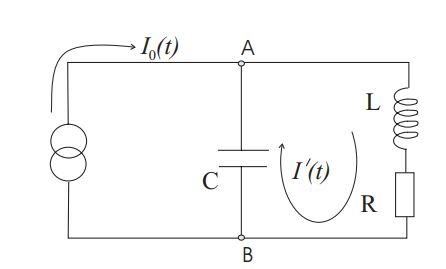
\includegraphics[scale=0.5]{TP1_Q2_G.JPG}
\end{figure}
\end{qns}
\begin{ans}
The impedance of the circuit in the frequency domain is 
$$\frac{1}{Z}=\frac{1}{Z_C}+\frac{1}{Z_L+Z_R}=i\omega C+\frac{1}{i\omega L+R}=\frac{i\omega RC-\omega^2LC+1}{R+i\omega L}$$
In temporal domain,
$$Z(t)=\int Z(\omega)e^{i\omega t}\frac{d\omega}{2\pi}=\int\frac{R+i\omega L}{i\omega RC-\omega^2LC+1}e^{i\omega t}\frac{d\omega}{2\pi}$$
The poles occur at $-\omega^2LC+i\omega RC+1=0$
$$\implies\omega_\pm=\frac{-iRC\pm\sqrt{-R^2C^2-4(-LC)}}{-2LC}=\frac{iR}{2L}\pm\sqrt{\frac{1}{LC}-\frac{R^2}{4L^2}}$$
We require light damping in order to have sinusodial response, i.e. $R^2<4L/C$. Hence, both poles $\omega_\pm$ lie in the upper half-plane. We have to impose causality $Z(t<0)=0$. Now, to invoke Jordan's Lemma, we require $\omega t>0$, so close the lower and upper half-planes for $t<0$ and $t>0$ respectively. No poles are enclosed in the lower half-plane, so by Cauchy's residue theorem, $Z(t<0)=0$ (consistent with causality). For $t>0$,
\begin{align}
    Z(t>0)&=-\frac{2\pi i}{2\pi}\bigg[\res_{\omega=\omega_+}\frac{R+i\omega L}{(\omega-\omega_+)(\omega-\omega_-)}e^{i\omega t}+\res_{\omega=\omega_-}\frac{R+i\omega L}{(\omega-\omega_+)(\omega-\omega_-)}e^{i\omega t}\bigg]\nonumber\\&=-\frac{i}{\omega_+-\omega_-}\bigg[(R+i\omega_+L)e^{i\omega_+t}-(R+i\omega_-L)e^{i\omega_-t}\bigg]\nonumber
\end{align}
The voltage response (due to an input current) is $V(\omega)=Z(\omega)I(\omega)$. By the convolution theorem, $V(t)=\int Z(t')I(t-t')dt'$, where $I(t)=I_0\Theta(t)\text{Re}[e^{i\Omega t}]$. So
\begin{align}
    V(t)&=-\frac{iI_0}{\omega_+-\omega_-}\bigg[\int_0^t(R+i\omega_+L)e^{i(\omega_+-\Omega)t'}e^{i\Omega t}-(R+i\omega_-L)e^{-i(\omega_--\Omega)t'}e^{i\Omega t}dt'\bigg]\nonumber\\&=\frac{-iI_0}{2\sqrt{\frac{1}{LC}-\frac{R^2}{4L^2}}}\text{Re}\bigg[e^{i\Omega t}\int_0^t(R+i\omega_+L)e^{i(\omega_+-\Omega)t'}-(R+i\omega_-L)e^{i(\omega_--\Omega)t'}dt'\bigg]\nonumber\\&=-\frac{I_0}{2\sqrt{\frac{1}{LC}-\frac{R^2}{4L^2}}}\text{Re}\bigg\{e^{i\Omega t}\bigg[\frac{(R+i\omega_+L)e^{i(\omega_+-\Omega)t'}}{\omega_+-\Omega}-\frac{(R+i\omega_-L)e^{i(\omega_--\Omega)t'}}{\omega_--\Omega}\bigg]_0^t\bigg\}\nonumber
\end{align}
The solution is a superposition of the steady state response (at $t'=0$) and the transient response (at $t'=t$). 
\end{ans}
\newpage
\begin{qns}
The Green’s function for a quantum-mechanical particle with Hamiltonian $H$ is defined by
$$\bigg(i\hbar\frac{\partial}{\partial t}-H\bigg)G(\mathbf{r},\mathbf{r'};t,t')=\delta^{(3)}(\mathbf{r}-\mathbf{r'})\delta(t-t')$$
Use Fourier methods to derive the Green’s function
$$G(\mathbf{r},\mathbf{r'};z)=\int e^{iz(t-t')/\hbar}G(\mathbf{r},\mathbf{r'};t,t')dt$$
for a non-relativistic free particle in three dimensions ($H=-\hbar^2\nabla^2/2m$), with $z=E+i\varepsilon$ for the four cases
$$(i)E>0,\varepsilon>0;~(ii)E>0,\varepsilon<0;~(iii)E<0,\varepsilon>0;~(iv)E<0,\varepsilon<0$$
The parameter $\varepsilon$ should be assumed to be real and small. Use your results to show that
$$\Delta G(\mathbf{r},\mathbf{r'};E)=-2\pi i\frac{2m}{\hbar^2}\frac{\sin(\sqrt{2mE}|\mathbf{r}-\mathbf{r'}|/\hbar)}{4\pi^2|\mathbf{r}-\mathbf{r'}|}\Theta(E)$$
where 
$$\Delta G(\mathbf{r},\mathbf{r'};E)=\lim_{\varepsilon\rightarrow 0}[G(\mathbf{r},\mathbf{r'};E+i|\varepsilon|)-G(\mathbf{r},\mathbf{r'};E-i|\varepsilon|)]$$
Calculate the density of states (the number of quantum states per unit energy per unit volume) $\rho(E)$ for a non-relativistic free particle in three dimensions using a simple phase space argument. Hence show that for this case
$$\rho(E)=\lim_{r\rightarrow r'}\frac{\Delta G(\mathbf{r},\mathbf{r'};E)}{-2\pi i}$$
Now consider the general case. For a system with Hamiltonian $H$, energy eigenvalues $E_n$ and corresponding eigenfunctions $\phi_n(r)$, show that
$$G(\mathbf{r},\mathbf{r'};z)=\sum_n\frac{\phi_n(\mathbf{r})\phi_n^*(\mathbf{r'})}{z-E_n}$$
Use this expression and the identity
$$\lim_{y\rightarrow 0^+}\frac{1}{x\pm iy}=\mathbb{P}\frac{1}{x}\mp i\pi\delta(x)$$
to show in general that
$$\rho(\mathbf{r};E)=\lim_{r\rightarrow r'}\frac{\Delta G(\mathbf{r},\mathbf{r'};E)}{-2\pi i}$$
\end{qns}
\begin{ans}
For the given expression, take FT with respect to $t$:
\begin{eqnarray}
\int\bigg(i\hbar\frac{\partial}{\partial t}-H\bigg)e^{iz(t-t')/\hbar}G(\mathbf{r},\mathbf{r'};t,t')dt&=&\delta^{(3)}(\mathbf{r}-\mathbf{r'})\int e^{iz(t-t')/\hbar}\delta(t-t')dt\nonumber\\
\frac{z}{\hbar}\hbar G(\mathbf{r},\mathbf{r'};z)+\frac{\hbar^2}{2m}\nabla^2G(\mathbf{r},\mathbf{r'};z)&=&\delta^{(3)}(\mathbf{r}-\mathbf{r'})\nonumber
\end{eqnarray}
Now, perform FT with respect to $\mathbf{r}$:
\begin{eqnarray}
\int\bigg(z+\frac{\hbar^2}{2m}\nabla^2\bigg)G(\mathbf{r},\mathbf{r'};z)e^{-i\mathbf{k}\cdot(\mathbf{r}-\mathbf{r'})}d^3\mathbf{r}&=&\int\delta^{(3)}(\mathbf{r}-\mathbf{r'})e^{-i\mathbf{k}\cdot(\mathbf{r}-\mathbf{r'})}d^3\mathbf{r}\nonumber\\\bigg(z-\frac{\hbar^2k^2}{2m}\bigg)G(\mathbf{k};z)&=&1\nonumber
\end{eqnarray}
The response function is thus $G(\mathbf{k};z)=\frac{1}{z-\hbar^2k^2/2m}$. Using FT to express it in real space:
\begin{align}
    G(\mathbf{r},\mathbf{r'};z)&=\int G(\mathbf{k};z)e^{i\mathbf{k}\cdot(\mathbf{r}-\mathbf{r'})}\frac{d^3k}{(2\pi)^3}\nonumber\\&=\int\frac{e^{i\mathbf{k}\cdot(\mathbf{r}-\mathbf{r'})}}{z-\frac{\hbar^2k^2}{2m}}\frac{k^2\sin\theta d\theta d\phi dk}{(2\pi)^3}\nonumber\\&=\frac{1}{(2\pi)^2}\int_0^\infty\frac{k^2}{z-\frac{\hbar^2k^2}{2m}}\int_0^\pi\sin\theta e^{ik(r-r')\cos\theta}d\theta dk\nonumber\\&=\frac{1}{(2\pi)^2}\int_0^\infty\frac{k^2}{z-\frac{\hbar^2k^2}{2m}}\bigg[\frac{e^{ik(r-r')}-e^{-ik(r-r')}}{ik(r-r')}\bigg]dk\nonumber\\&=\frac{1}{(2\pi)^2}\int_0^\infty\frac{k^2}{z-\frac{\hbar^2k^2}{2m}}\frac{2i\sin(k(r-r'))}{ik(r-r')}dk\nonumber\\&=\frac{1}{(2\pi)^2}\int_{-\infty}^\infty\frac{k}{z-\frac{\hbar^2k^2}{2m}}\frac{\sin(k(r-r'))}{r-r'}dk\nonumber
\end{align}
The poles are at $\frac{2mz}{\hbar^2}-k^2=0\implies k=\pm\frac{\sqrt{2mz}}{\hbar}$ on the real axis. We will need to translate the poles accordingly, via $z=E+i\varepsilon$ for some $\varepsilon$ for both $E>0$ and $E<0$. When closing either half-plane, we invoke Jordan's Lemma (which requires $k(r-r')>0$. When $r-r'>0$ (physically), close the upper half-plane.
\begin{enumerate}
    \item Consider first, $E>0$. If $z=E+i\varepsilon$, then 
    $$k_\pm=\pm\frac{\sqrt{2m}}{\hbar}E^{1/2}e^{i\varepsilon/2}$$
    since $(E^{1/2}e^{i\varepsilon/2})^2\approx E+i\varepsilon$, with $\varepsilon$ small. Only the pole at $k_+$ is enclosed. By Cauchy's residue theorem:
    \begin{align}
        G(\mathbf{r},\mathbf{r'};z)&=\frac{-i}{2\pi}\frac{2m}{|\mathbf{r}-\mathbf{r'}|\hbar^2}\frac{k_+\sin k_+|\mathbf{r}-\mathbf{r'}|}{k_+-k_-}\nonumber\\&=-\frac{i}{2\pi}\frac{2m}{|\mathbf{r}-\mathbf{r'}|\hbar^2}\frac{\sqrt{2mE}\sin(\sqrt{2mE}|\mathbf{r}-\mathbf{r'}|/\hbar)}{2\sqrt{2mE}}\nonumber\\&=\frac{-im}{2\pi|\mathbf{r}-\mathbf{r'}|\hbar^2}\sin\frac{\sqrt{2mE}}{\hbar}|\mathbf{r}-\mathbf{r'}|\nonumber
    \end{align}
    If $z=E-i\varepsilon$, then $k_\pm=\pm\frac{\sqrt{2m}}{\hbar}E^{1/2}e^{-i\varepsilon/2}$. Only the pole at $k_-$ is enclosed. Again, by Cauchy's residue theorem:
    $$G(\mathbf{r},\mathbf{r'};z)=\frac{im}{2\pi|\mathbf{r}-\mathbf{r'}|\hbar^2}\sin\frac{\sqrt{2mE}}{\hbar}|\mathbf{r}-\mathbf{r'}|$$
    Hence, for $E>0$, $\Delta G$ is
    $$\Delta G(\mathbf{r},\mathbf{r'};E)=\lim_{\varepsilon\rightarrow 0}[G(\mathbf{r},\mathbf{r'};E+i\varepsilon)-G(\mathbf{r},\mathbf{r'};E-i\varepsilon)]=-\frac{im}{\pi\hbar^2|\mathbf{r}-\mathbf{r'}|}\sin\frac{\sqrt{2mE}}{\hbar}|\mathbf{r}-\mathbf{r'}|$$
    \item When $E<0$, the sign of $\varepsilon$ does not matter. There will only be one pole at $k_+$ in the upper half-plane and the other in the lower half-plane. The residue at $k_+$ will give the response to be:
    $$G(\mathbf{r},\mathbf{r'};z)=\frac{-im}{\pi|\mathbf{r}-\mathbf{r'}|\hbar^2}\sin\frac{\sqrt{2mE}}{\hbar}|\mathbf{r}-\mathbf{r'}|$$
    So, the difference $\Delta G$ is zero. 
\end{enumerate}
We thus have $\Delta G$ to be non-zero only in $E>0$. By introducing the heaviside function $\Theta(E)$, the desired answer follows.\\[5pt]
The number of states (per unit volume) in a sphere of radius $k$ in phase space is
$$n=\frac{1}{(2\pi)^3}\frac{4\pi}{3}k^3$$
The density of states is then
$$\rho(E)=\frac{dn}{dE}=\frac{dn}{dk}\frac{dk}{dE}=\frac{1}{(2\pi)^3}4\pi \frac{2mE}{\hbar^2}\frac{\sqrt{2m}}{2\hbar\sqrt{E}}=\frac{1}{2\pi^2}\frac{m\sqrt{2mE}}{\hbar^3}$$
This is indeed equal to $\lim_{r\rightarrow r'}\frac{\Delta G(\mathbf{r},\mathbf{r'};E)}{-2\pi i}$ (using L'Hopital rule). For the generic case, take the expression $G$ satisfies and multiply by $\phi_n^*(\mathbf{r})$ from the left, before taking a Hermitian conjugate (so the operator $H$ acts on $\phi_n(\mathbf{r})$:
\begin{eqnarray}
(z-H)G(\mathbf{r}-\mathbf{r'};z)&=&\delta^{(3)}(\mathbf{r}-\mathbf{r'})\nonumber\\\bigg[\int\phi_n^*(\mathbf{r})(z-H)G(\mathbf{r}-\mathbf{r'};z)d^3\mathbf{r}\bigg]^\dag&=&\bigg[\int\phi_n^*(\mathbf{r})\delta^{(3)}(\mathbf{r}-\mathbf{r'})d^3\mathbf{r}\bigg]^\dag\nonumber\\\int G(\mathbf{r}-\mathbf{r'};z)(z-E_n)\phi_n(\mathbf{r})d^3\mathbf{r}&=&\phi_n(\mathbf{r'})\nonumber
\end{eqnarray}
Next, we multiply by $\phi_n(\mathbf{r'})$ and sum over all states:
$$\int\sum_n\phi_n(\mathbf{r})\phi_n(\mathbf{r''})G(\mathbf{r}-\mathbf{r'};z)d^3\mathbf{r}=\sum_n\frac{\phi_n(\mathbf{r'})\phi_n^*(\mathbf{r''})}{z-E_n}\implies G(\mathbf{r''}-\mathbf{r};z)=\sum_n\frac{\phi_n(\mathbf{r'})\phi_n^*(\mathbf{r''})}{z-E_n}$$
where $\sum_n\phi_n(\mathbf{r}\phi_n(\mathbf{r''})=\delta^{(3)}(\mathbf{r}-\mathbf{r''})$. Given the identity, we can write:
$$\delta(E-E_n)=\frac{1}{2i\pi}\bigg(\frac{1}{E-E_n-i\varepsilon}-\frac{1}{E-E_n+i\varepsilon}\bigg)$$
The density of states is then by definition:
\begin{align}
    \rho(\mathbf{r},\mathbf{r'};E)&=\sum_n\phi_n(\mathbf{r})\phi_n^*(\mathbf{r'})\delta(E-E_n)\nonumber\\&=\sum_n\phi_n(\mathbf{r})\phi_n^*(\mathbf{r'})\frac{1}{2i\pi}\bigg(\frac{1}{E-E_n-i\varepsilon}-\frac{1}{E-E_n+i\varepsilon}\bigg)\nonumber\\&=\frac{1}{2i\pi}\bigg[G_{0^-}(\mathbf{r},\mathbf{r'};E)-G_{0^+}(\mathbf{r},\mathbf{r'};E)\bigg]\nonumber\\&=-\frac{1}{2\pi i}\Delta G(\mathbf{r},\mathbf{r'};E)\nonumber
\end{align}
\end{ans}
\newpage
\begin{qns}
The equation of motion for a damped harmonic oscillator has the form:
$$\ddot{x}+\gamma\dot{x}+\omega_0^2x=f(t)$$
Derive an expression for the Fourier Transform of the Green’s function $G(\omega)$ and write down the Kramers-Kronig relations for its real and imaginary parts.\\[5pt]
Convert the principal-value integrals to contour integrals and find their poles. By evaluating one of these integrals show that the corresponding Kramers-Kronig relation is obeyed by this Green’s function.\\[5pt]
[Hint: $\mathbb{P}\int_{-\infty}^\infty f(x)dx=\lim_{\varepsilon\rightarrow 0}[\int_{-\infty}^{-\varepsilon}+\int_\varepsilon^\infty]f(x)dx$ for a pole at $x=0$.]
\end{qns}
\begin{ans}
The corresponding Green's function satisfies
$$\frac{\partial^2G(t,t')}{\partial t^2}+\gamma\frac{\partial G(t,t')}{\partial t}+\omega_0^2G(t,t')=\delta(t-t')$$
Take Fourier transform of the equation:
$$(-\omega^2-i\gamma\omega+\omega_0^2)G(\omega)=1$$
The poles occur at $-\omega^2-i\gamma\omega+\omega_0^2=0\implies\omega_\pm=-\frac{\gamma i}{2}\pm\sqrt{\omega_0^2-(\gamma/2)^2}:=\pm a-ib$. For oscillatory solutions, we impose $\omega_0>\gamma/2$. The Green's function is then
$$G(\omega)=\frac{-1}{(\omega-\omega_+)(\omega-\omega_-)}=\frac{-1}{(\omega^2-a^2-b^2)+2ib\omega}=\frac{-(\omega^2-a^2-b^2)+2ib\omega}{(\omega-a+ib)(\omega+a+ib)(\omega-a-ib)(\omega+a-ib)}$$
The Kramers-Kronig relation is
$$\mathcal{P}\int_{-\infty}^\infty\text{Im}\bigg[\frac{G(\omega)}{\omega-\xi}\bigg]d\omega=\pi\text{Re}[G(\xi)]=\pi\frac{-(\omega^2-a^2-b^2)}{(\omega-a+ib)(\omega+a+ib)(\omega-a-ib)(\omega+a-ib)}$$
Convert the principal-value integrals to contour integrals. Only the poles $\omega=\pm a+ib$ are in the upper half-plane (necessary for Kramers-Kronig relation) which will be enclosed. The contribution due to $\omega=\xi$ (on real axis) will be half the usual contribution. Using Cauchy's residue theorem, we obtain the LHS, which is indeed equal to the RHS.
\end{ans}
\newpage
\subsection{Tripos Questions}
\subsubsection*{2016 Q3}
\begin{qns}
Consider the Klein-Gordon Lagrangian density for a complex scalar field in Minkowski space, coupled to an external vector potential $A_\mu$ and to a time-dependent driving force $f(t)$:
$$\mathcal{L}=(\partial_\mu\phi^*)(\partial^\mu\phi)-m^2\phi^*\phi+ieA_\mu[\phi\partial^\mu\phi^*-\phi^*\partial^\mu\phi]+f(t)(\phi+\phi^*)$$
where $A_\mu=(V(\mathbf{r}),0,0,0)$ and $V(\mathbf{r})$ is a real function of the space coordinates $\mathbf{r}$ but is independent of time.
\begin{enumerate}[label=(\alph*)]
\item Show that the Euler-Lagrange equations can be written as
$$\partial_\mu\partial^\mu\phi+2ieA^\mu(\mathbf{r})\partial_\mu\phi+m^2\phi=f(t)$$
and equivalently for $\phi^*$. \hfill\textbf{[5]}
\item The Green’s function $\mathcal{G}(\mathbf{r},\mathbf{r'};t,t')$ is a solution of the above equation of motion when the right hand side is replaced by $\delta(t-t')\delta^{(3)}(\mathbf{r}-\mathbf{r'})$. Using the following sign convention for the Fourier transform,
$$\mathcal{G}(\mathbf{r},\mathbf{r'};t,t')=\int\int G(\mathbf{k};\omega)e^{-i\omega(t-t')+i\mathbf{k}\cdot(\mathbf{r}-\mathbf{r'})}\frac{d^3k}{(2\pi)^3}\frac{d\omega}{2\pi}$$
show that $G(\mathbf{k};\omega)$ satisfies the equation
$$[-\omega^2+k^2+m^2]G(\mathbf{k};\omega)+2e\omega\int V(\mathbf{k}-\mathbf{k'})G(\mathbf{k'};\omega)\frac{d^3k'}{(2\pi)^3}=1$$
where $V(\mathbf{k}-\mathbf{k'})=\int V(\mathbf{r})e^{-i(\mathbf{k}-\mathbf{k'})\cdot(\mathbf{r}-\mathbf{r'})}d^3r$.\hfill\textbf{[8]}
\item Consider the case where $V(\mathbf{k}-\mathbf{k'})=-(2\pi)^3i\gamma\delta^{(3)}(\mathbf{k}-\mathbf{k'})$, $\gamma$ real and positive. Show that one can then obtain $G(\mathbf{k};t,t')$ from the integral\hfill\textbf{[3]}
$$G(\mathbf{k};t,t')=\int\frac{e^{-i\omega(t-t')}}{-\omega^2-2e\gamma i\omega+k^2+m^2}\frac{d\omega}{2\pi}$$
Discuss the location of the poles as a function of $\mathbf{k}$, for fixed $m$, $e$, and $\gamma$. Draw schematically where they appear in the complex $\omega$ plane for $k^2+m^2>e^2\gamma^2$ and for $k^2+m^2<e^2\gamma^2$.\hfill\textbf{[6]}
\item Assume that $k^2+m^2>e^2\gamma^2$.  Using contour integration and Cauchy’s theorem, compute $G(\mathbf{k};t,t')$ for $t>t'$ as well as $t<t'$. Justify your choice of contour in each case. \hfill\textbf{[3]}
\end{enumerate}
\end{qns}
\begin{ans}\leavevmode
\begin{enumerate}[label=(\alph*)]
\item We have
$$\frac{\partial\mathcal{L}}{\partial\phi}=-m^2\phi^*+ieA_\mu\partial^\mu\phi^*+f(t),\quad\partial_\mu\bigg(\frac{\partial\mathcal{L}}{\partial(\partial_\mu\phi)}\bigg)=\partial_\mu\partial^\mu\phi^*-ie\phi^*\partial_\mu A^\mu-ieA^\mu\partial_\mu\phi^*$$
$$\frac{\partial\mathcal{L}}{\partial\phi^*}=-m^2\phi-ieA_\mu\partial^\mu\phi+f(t),\quad\partial_\mu\bigg(\frac{\partial\mathcal{L}}{\partial(\partial_\mu\phi^*)}\bigg)=\partial_\mu\partial^\mu\phi+ie\phi\partial_\mu A^\mu-ieA^\mu\partial_\mu\phi$$
The equations of motion follow from the Euler-Lagrange equations:
$$\partial_\mu\partial^\mu\phi+2ieA^\mu(\mathbf{r})\partial_\mu\phi+m^2\phi=f(t),\quad\partial_\mu\partial^\mu\phi^*-2ieA^\mu(\mathbf{r})\partial_\mu\phi^*+m^2\phi^*=f(t)$$
\item The corresponding Green's function satisfies
$$(\partial_0^2-\nabla^2+2ieV(\mathbf{r})\partial_0+m^2)\mathcal{G}(\mathbf{r},\mathbf{r'};t,t')=\delta(t-t')\delta^{(3)}(\mathbf{r}-\mathbf{r'})$$
Firstly, write $\mathcal{G}$ in terms of $G$:
\begin{eqnarray}
\delta(t-t')\delta^{(3)}(\mathbf{r}-\mathbf{r'})&=&\int\int(\partial_0^2-\nabla^2+2ieV(\mathbf{r})\partial_0+m^2)G(\mathbf{k};\omega)e^{-i\omega(t-t')+i\mathbf{k}\cdot(\mathbf{r}-\mathbf{r'})}\frac{d^3k}{(2\pi)^3}\frac{d\omega}{2\pi}\nonumber\\&=&\int\int(-\omega^2+k^2+m^2+2eV(\mathbf{r})\omega)G(\mathbf{k};\omega)e^{-i\omega(t-t')+i\mathbf{k}\cdot(\mathbf{r}-\mathbf{r'})}\frac{d^3k}{(2\pi)^3}\frac{d\omega}{2\pi}\nonumber
\end{eqnarray}
Next, do FT with respect to $t$ and $r$:
\begin{eqnarray}
&&\int\delta(t-t')e^{i\omega_0(t-t')}dt\int\delta(\mathbf{r}-\mathbf{r'})e^{-i\mathbf{k_0}\cdot(\mathbf{r}-\mathbf{r'})}d^3r\nonumber\\&=&\int\int\int\int(-\omega^2+k^2+2eV(\mathbf{r})\omega+m^2)G(\mathbf{k};\omega)e^{-i(\omega-\omega_0)(t-t')+i(\mathbf{k}-\mathbf{k_0})\cdot(\mathbf{r}-\mathbf{r'})}\frac{d^3k}{(2\pi)^3}\frac{d\omega}{2\pi}dtd^3r\nonumber\\1&=&
(-\omega_0^2+k_0^2+m^2)G(\mathbf{k_0};\omega_0)+2e\omega_0\int\int V(\mathbf{r})e^{-i(\mathbf{k_0}-\mathbf{k})\cdot(\mathbf{r}-\mathbf{r'})}V(\mathbf{r})G(\mathbf{k_0};\omega_0)\frac{d^3k}{(2\pi)^3}d^3\mathbf{r'}\nonumber\\&=&(-\omega_0^2+k_0^2+m^2)G(\mathbf{k_0};\omega_0)+2e\omega_0\int V(\mathbf{k_0}-\mathbf{k})G(\mathbf{k};\omega_0)\frac{d^3k}{(2\pi)^3}\nonumber
\end{eqnarray}
Relabel indices to get the desired result.
\item 
$$1=(-\omega^2+k^2+m^2)G(\mathbf{k};\omega)-2e\omega\int i\gamma\delta^{(3)}(\mathbf{k}-\mathbf{k'})G(\mathbf{k'};\omega)d^3k'=(-\omega^2+k^2+m^2-2e\omega i\gamma)G(\mathbf{k};\omega)$$
Hence, by a Fourier transform,
$$G(\mathbf{k};t,t')=\int_{-\infty}^\infty\frac{e^{-i\omega(t-t')}}{-\omega^2+k^2+m^2-2e\omega i\gamma}\frac{d\omega}{2\pi}$$
The poles occur at $0=-\omega^2+k^2+m^2-2e\omega i\gamma$:
$$\omega_\mp=-ei\gamma\mp\sqrt{-e^2\gamma^2+(k^2+m^2)}$$
When $-e^2\gamma^2+k^2+m^2>0$, the two simple poles occur in the lower half-plane. When $-e^2\gamma^2+k^2+m^2<0$, the two simple poles occur along the $\text{Im}[\omega]$ axis.
\item To evaluate the contour integral, we have to invoke Jordan's Lemma such that the contribution by the circular arc vanishes (must have $-\omega(t-t')>0$). For $t<t'$ and $t>t'$, we have to close the upper (anti-clockwise) and lower half-plane (clockwise) respectively. Since no poles are enclosed in the former, $G(\mathbf{k};t<t')=0$, consistent with causality. For the latter, both simple poles are enclosed. By Cauchy's residue theorem,
\begin{align}
    G(\mathbf{k};t>t')&=-(-1)\frac{2\pi i}{2\pi}\bigg[\frac{e^{-i\omega_+(t-t')}}{\omega_+-\omega_-}+\frac{e^{-i\omega_-(t-t')}}{\omega_--\omega_+}\bigg]\nonumber\\&=\frac{-ie^{-e\gamma(t-t')}}{2\sqrt{k^2+m^2-e^2\gamma^2}}2i\sin[\sqrt{k^2+m^2-e^2\gamma^2}(t-t')]\nonumber
\end{align}
where we incurred a minus sign for a clockwise contour.
\end{enumerate}
\end{ans}
\newpage
\subsubsection*{2017 Q4}
\begin{qns}
A charged particle radiates energy at a rate proportional to the square of its
acceleration, $\ddot{x}^2$. For periodic motion, this is equivalent to the action of a force $\dddot{x}$ on the particle. If we consider simple harmonic oscillations in one dimension, the equation of motion can then be written as
$$\ddot{x}+x-\varepsilon\dddot{x}=f(t),\quad\varepsilon\in\mathbb{R}$$
where $f(t)$ is an external driving force.
\begin{enumerate}[label=(\alph*)]
\item Obtain an expression for the Green’s function $G(\omega)$ such that the Fourier transform of the solution of the equation of motion can be written as $x(\omega) = G(\omega)f(\omega)$.\hfill\textbf{[4]}\\[5pt]
Discuss in general what conditions $G(t − t')$ must satisfy in order to respect
causality, and how this relates to the position of the poles of $G(\omega)$ in the complex $\omega$ plane. \hfill\textbf{[4]}

\begin{mdframed}
\textcolor{darkblue}{Use the Fourier transform convention:}
$$G(t-t')=\int G(\omega)e^{-i\omega(t-t')}\frac{d\omega}{2\pi}$$
\end{mdframed}
\item Find the two poles $\omega^{(0)}_{1,2}$ for $\varepsilon=0$ and show how they are affected to leading order in $\varepsilon$ by the addition of the term $-\varepsilon\dddot{x}$ in the equation of motion.\hfill\textbf{[7]}\\[5pt]
Discuss causality in relation to the sign of $\varepsilon$. How does it compare to the case considered in the lecture notes of a damped simple harmonic oscillator $\ddot{x}+x − \varepsilon\dot{x} = f(t)$?\hfill\textbf{[5]}

\begin{mdframed}
\textcolor{darkblue}{You may assume that the poles move, to leading order, by an amount proportional to $\varepsilon$.}
\end{mdframed}
\item Show that, to leading order, a third pole of $G(\omega)$ can be found of the
form $\omega_3\approx\alpha_3/\varepsilon$. Find the value of the constant $\alpha_3$ and discuss whether this solution is compatible with causality.

\hfill\textbf{[5]}
\end{enumerate}
\end{qns}
\begin{ans}\leavevmode
\begin{enumerate}[label=(\alph*)]
\item The corresponding Green's function satisfies
$$\frac{\partial^2G(t,t')}{\partial t^2}+G(t,t')-\varepsilon\frac{\partial^3G(t,t')}{\partial t^3}=\delta(t-t')$$
Write $G(t,t')$ in terms of $G(\omega)$:
\begin{align}
\int(-\omega^2+1-i\varepsilon\omega^3)G(\omega)e^{-i\omega(t-t')}\frac{d\omega}{2\pi}&=\delta(t-t')\nonumber\\\int(-\omega^2+1-i\varepsilon\omega^3)G(\omega)e^{-i(\omega-\omega_0)(t-t')}\frac{d\omega}{2\pi}dt&=\int\delta(t-t')e^{i\omega_0(t-t')}dt\nonumber\\(-\omega_0^2+1-i\varepsilon\omega_0^3)G(\omega_0)=1\nonumber
\end{align}
So, the Green's function is $G(\omega)=\frac{1}{-\omega^2+1-i\varepsilon\omega^3}$. Perform a Fourier transform:
$$G(t-t')=\int G(\omega)e^{-i\omega(t-t')}\frac{d\omega}{2\pi}$$
This is evaluated using the contour integration method. $\gamma$ is a semi-circular contour that closes one of the two half-planes. In order for the contribution due to the semi-circular arc to vanish, we have to invoke Jordan's Lemma (which requires $-\omega(t-t')>0$). So we close the upper (counter-clockwise) and lower (clockwise) half-planes respectively for $t<t'$ and $t>t'$. To respect causality, we must have $G(t<t')=0$. This means there must be no poles enclosed when we close the upper half-plane. So all the poles of $G(\omega)$ must lie in the lower half-plane.
\item When $\varepsilon=0$, we have $\omega^{(0)}_{1,2}=\pm1$. With the hint, let $\omega_{1,2}\approx \pm1+\alpha_{1,2}$ for $\alpha_{1,2}$ small:
$$-(\alpha_{1,2}^2+1\pm2\alpha_{1,2})+1+i\varepsilon(\alpha_{1,2}^3\pm 3\alpha_{1,2}^2+3\alpha_{1,2}\pm1)=0\implies\alpha_{1,2}=-i\varepsilon/2$$
which is indeed proportional to $\varepsilon$. Again, poles must be in the lower half-plane so the poles $\omega_{1,2}^{(0)}$ originally on the real axis must be shifted vertically downwards, hence $\varepsilon>0$.\\[5pt]
Compared ot the damped simple harmonic oscillator, the first order dissipative terms are opposite in sign with respect to the third order dissipative terms considered here.
\item Try $\omega_3\approx\alpha_3/\varepsilon$, then
$$0=-\frac{\alpha_3^2}{\varepsilon^2}+1-i\varepsilon\frac{\alpha_3^3}{\varepsilon^3}=\frac{\alpha_3^2}{\varepsilon^2}(-1-i\alpha_3)+1$$
When $\varepsilon$ is small, $\frac{\alpha_3^3}{\varepsilon^2}(i+1)$ is large, so this dominates over 1, and thus $\alpha_3=i$. We must have $\omega_3\approx i/\varepsilon$. For $\varepsilon>0$, we have $\omega_3$ to be in the upper half-plane. This violates with causality. This is expected from a relativistic system (radiation emitted by an accelerating particle is a relativistic effect).
\begin{center}
    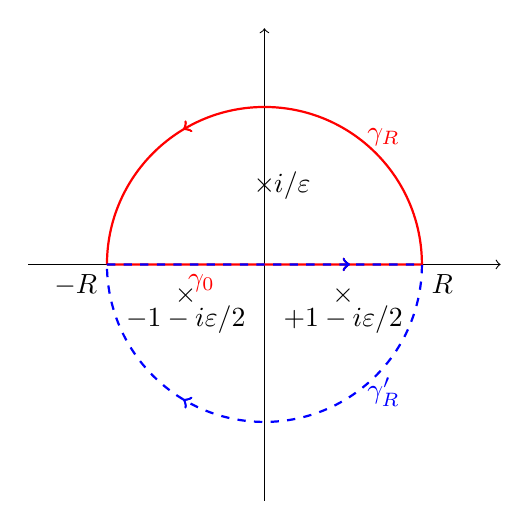
\begin{tikzpicture}
      \draw [->] (-3, 0) -- (3, 0);
      \draw [->] (0, -3) -- (0, 3);

      \draw [red, thick, ->-=0.3, ->-=0.8] (-2, 0) -- (2, 0) node [pos=0.3, below] {$\gamma_0$} arc(0:180:2) node [pos=0.3, right] {$\gamma_R$};
      \draw [dashed, blue, thick, ->-=0.3, ->-=0.8] (-2, 0) -- (2, 0) arc(0:-180:2) node [pos=0.3, right] {$\gamma_R'$};

      \node [anchor = north east] at (-2, 0) {$-R$};
      \node [anchor = north west] at (2, 0) {$R$};

      \node at (0, 1) {$\times$};
      \node at (1, -0.4) {$\times$};
      \node at (-1, -0.4) {$\times$};
      \node [right] at (0, 1) {$i/\varepsilon$};
      \node [below] at (-1, -0.4) {$-1-i\varepsilon/2$};
      
      \node [below] at (1, -0.4) {$+1-i\varepsilon/2$};
    \end{tikzpicture}
  \end{center}
\end{enumerate}
\end{ans}
\newpage
\subsubsection*{2018 Q4}
\begin{qns}
Consider the Lagrangian density of a 1-dimensional elastic rod with density $\rho=1$ and elastic constant $\kappa=1$,
$$\mathcal{L}=\frac{1}{2}\bigg(\frac{\partial\phi}{\partial t}\bigg)^2-\frac{1}{2}\bigg(\frac{\partial\phi}{\partial x}\bigg)^2$$
where $\phi(x, t)$ is the local displacement field.
\begin{enumerate}[label=(\alph*)]
\item Obtain the Euler-Lagrange equations of motion for the field.\hfill\textbf{[3]}
\item Obtain the total angular momentum tensor of the system. Is it conserved? Justify your answer and comment briefly on its significance in relation to the symmetries of the system.

\hfill\textbf{[7]}
\item Consider adding a viscous damping term to the equation of motion of the rod, $\gamma\partial_t\partial_x^2\phi$ where $\gamma$ is a positive constant. Obtain the Fourier transform $\hat{G}(k,\omega)$ of the corresponding Green’s function $G(x, t)$, which solves the equation of motion with a delta function driving in space and time:\hfill\textbf{[5]}
$$\bigg(-\frac{\partial^2}{\partial t^2}+\frac{\partial^2}{\partial x^2}+\gamma\frac{\partial}{\partial t}\frac{\partial^2}{\partial x^2}\bigg)G(x,t)=\delta(x)\delta(t)$$
\begin{mdframed}
\textcolor{darkblue}{Use the Fourier transform conventions:}
$$\tilde{G}(k,t)=\int\hat{G}(k,\omega)e^{-i\omega t}\frac{d\omega}{2\pi},\quad G(x,t)=\int\int\hat{G}(k,\omega)e^{-ikx-i\omega t}\frac{dkd\omega}{(2\pi)^2}$$
\end{mdframed}
\item Assuming that $k^2<4/\gamma^2$, obtain an expression for $\tilde{G}(k,t)$ by Cauchy integration. Then take the limit $\gamma\rightarrow 0$ and compute $G(x, t)$. Is the result consistent with the choice of initial conditions and with $\rho=\kappa$?\hfill\textbf{[10]}

\begin{mdframed}
\textcolor{darkblue}{You may need the integral:}
$$\frac{1}{\pi}\int_{-\infty}^\infty\frac{\sin s}{s}e^{-isx}ds=\text{TH}(x)$$
\textcolor{darkblue}{where $\text{TH}(x)$ is the top hat function, which takes value 1 for $-1<x<1$ and vanishes otherwise.}
\end{mdframed}
\end{enumerate}
\end{qns}
\begin{ans}\leavevmode
\begin{enumerate}[label=(\alph*)]
\item The Euler-Lagrange equation is
$$0=\frac{\partial\mathcal{L}}{\partial\phi}-\frac{d}{dt}\frac{\partial\mathcal{L}}{\partial\dot{\phi}}-\frac{d}{dx}\frac{\partial\mathcal{L}}{\partial(\partial\phi/\partial x)}=-\ddot{\phi}+\phi''$$
\item The total angular momentum tensor of the system is
$$J^{jk}=\int x^jT^{0k}-x^kT^{0j}dx$$
The stress-energy tensor components are
$$T^{01}=\frac{\partial\mathcal{L}}{\partial\dot{\phi}}\bigg(-\frac{\partial\phi}{\partial x}\bigg)=-\dot{\phi}\phi',\quad T^{10}=\frac{\partial\mathcal{L}}{\partial\phi'}\dot{\phi}=-\phi'\dot{\phi},\quad T^{00}=\frac{\partial\mathcal{L}}{\partial\dot{\phi}}\dot{\phi}-\mathcal{L}=\frac{1}{2}\dot{\phi}^2+\frac{1}{2}(\phi')^2$$
The total angular momentum tensor is anti-symmetric, so we just need to compute
$$J^{01}=x^0T^{01}-x^1T^{00}=-t\phi'\dot{\phi}-x\frac{1}{2}\dot{\phi}^2-\frac{1}{2}x(\phi')^2$$
Due to the choice of density and elastic constants of the beam, the stress-energy tensor $T^{\mu\nu}$ is symmetric in $\mu$ and $\nu$. $x^\mu T^{\lambda\nu}-x^\nu T^{\lambda\mu}$ can be shown to be conserved:
$$\partial_\lambda(x^\mu T^{\lambda\nu}-x^\nu T^{\lambda\mu})=\tensor*{\delta}{*_{}^{\nu}_{\lambda}}T^{\lambda\nu}-\tensor*{\delta}{*_{}^{\nu}_{\lambda}}T^{\lambda\mu}=T^{\mu\nu}-T^{\nu\mu}$$
which is zero if $T^{\mu\nu}$ is symmetric. Hence, $J^{\mu\nu}$ is the corresponding conserved charge, i.e. $\partial_tJ^{\mu\nu}=0$.
\item For the given expression, the RHS is
$$\int\int\bigg(-\frac{\partial^2}{\partial t^2}+\frac{\partial^2}{\partial x^2}+\gamma\frac{\partial}{\partial t}\frac{\partial^2}{\partial x^2}\bigg)\hat{G}(k,\omega)e^{-ikx-i\omega t}\frac{dkd\omega}{(2\pi)^2}=\int\int(\omega^2-k^2+i\gamma\omega k^2)\hat{G}(k,\omega)e^{-ikx-i\omega t}\frac{dkd\omega}{(2\pi)^2}$$
Now, performing FT on both sides with respect to $x$ and $t$:
\begin{eqnarray}
\int\delta(x)e^{ik_0x}dx\int\delta(t)e^{i\omega_0t}dt&=&\int\int\int\int(\omega^2-k^2+i\gamma\omega k^2)\hat{G}(k,\omega)e^{-i(k-k_0)x}e^{-i(\omega-\omega_0)t}\frac{dkd\omega}{(2\pi)^2}dxdt\nonumber\\
1&=&\int\int\delta(k-k_0)\delta(\omega-\omega_0)(\omega^2-k^2+i\gamma\omega k^2)\hat{G}(k,\omega)dkd\omega\nonumber\\&=&
(\omega_0^2-k_0^2+i\gamma\omega_0k_0^2)\hat{G}(k_0,\omega_0)\nonumber
\end{eqnarray}
The result is $\hat{G}(k,\omega)=\frac{1}{\omega^2-k^2+i\gamma\omega k^2}$. 
\item The poles occur at $\omega^2-k^2+i\gamma\omega k^2=0$:
$$\omega_\pm=\frac{-i\gamma k^2\pm\sqrt{4k^2-\gamma^2k^4}}{2}$$
We have $k^2<4/\gamma^2\implies\sqrt{4k^2-\gamma^2k^4}>0$. The poles are thus first order poles in the upper half-plane. We thus evaluate $\tilde{G}(k,t)$ by Cauchy integration:
$$\tilde{G}(k,t)=\frac{1}{2\pi}\int\frac{e^{-i\omega t}d\omega}{\omega^2-k^2-i\gamma\omega k^2}=\frac{1}{2\pi}\int\frac{e^{-i\omega t}d\omega}{(\omega-\omega_+)(\omega-\omega_-)}$$
The Cauchy integration is evaluated using Jordan's Lemma (which requires $-i\omega t>0$ in order for the semi-circular contribution to vanish) and Cauchy's residue theorem (where we find the residues of the enclosed poles). For $t>0$ and $t<0$, we close the upper half-plane (anti-clockwise) and lower half-plane (clockwise) respectively. Since no poles are enclosed in the lower half-plane, we have $\tilde{G}(k,t<0)=0$, which is consistent with causality. For $t>0$, we compute the residues of the two enclosed simple poles:
\begin{align}
\tilde{G}(k,t)&=2\pi i\frac{1}{2\pi}\bigg[\frac{e^{-i\omega_+t}}{\omega_+-\omega-}+\frac{e^{-i\omega_-t}}{\omega_--\omega+}\bigg]\nonumber\\&=\frac{ie^{-\gamma k^2t/2}}{\sqrt{4k^2-\gamma^2k^4}}(2i\sin\sqrt{4k^2-\gamma^2k^4}t)\nonumber\\&=-\frac{2e^{-\gamma k^2t/2}}{\sqrt{4k^2-\gamma^2k^4}}\sin(\sqrt{4k^2-\gamma^2k^4}t)\nonumber
\end{align}
where $-i\omega_\pm t=-\frac{\gamma k^2}{2}t\mp it\sqrt{4k^2-\gamma^2k^4}$. In the limit of $\gamma\rightarrow 0$, $\tilde{G}(k,t)\rightarrow-\frac{\sin kt}{k}$. We have
$$G(x,t)=\int\tilde{G}(k,t)e^{-ikx}\frac{dk}{2\pi}=-\int\frac{\sin kt}{k}e^{-ikx}\frac{dk}{2\pi}=-\frac{1}{2}\text{TH}(x/t)$$
This is consistent with our initial conditions since $G(x,t)=0$ only at $x=0$ and $t=0$. Physically, the walls of $G(x,t)$ at $x=\pm t$ move with velocity 1 (for an elastic rod of $\rho=\kappa$).

\end{enumerate}
\end{ans}
\newpage
\subsubsection*{2020 Q4}
\begin{qns}
Consider the following Lagrangian density for a complex relativistic scalar
field
$$\mathcal{L}=(\partial_\mu\phi^*)(\partial^\mu\phi)+\frac{m^2}{2}(\phi^*\phi)^2-\frac{\lambda}{3}(\phi^*\phi)^3$$
where $m$ and $\lambda$ are real positive constants.
\begin{enumerate}[label=(\alph*)]
\item Derive the minimal energy state(s) of the field $\phi$ and obtain the Lagrangian density for small fluctuations $\chi$ about (one of) the minimum energy state(s), $\phi_0$, up to quadratic order in $\chi$. Discuss briefly the behaviour of the real and imaginary components of $\chi$.\hfill\textbf{[8]}
\item Consider coupling the complex scalar field $\phi$ in this question to an electromagnetic field via the covariant derivative. Discuss briefly what happens to the fluctuating complex field $\chi$ as a result.\hfill\textbf{[3]}
\item Write the Lagrangian density of such a coupled electromagnetic field when the complex scalar field is exactly at (one of) its minimum energy state(s). If needed, you may ignore irrelevant constant terms. Find the corresponding Euler-Lagrange equations of motion for the 4-vector potential, and show that (by an appropriate choice of gauge or otherwise) they can be written as\hfill\textbf{[6]}
$$\bigg(\partial_t^2-\partial_x^2+\frac{2e^2m^2}{\lambda}\bigg)A^\nu=0$$
in 1+1 space-time dimensions and natural units. You may use, without deriving it, the result:
$$\frac{\partial}{\partial(\partial_\mu A_\nu)}(F_{\alpha\beta}F^{\alpha\beta})=4F^{\mu\nu}\text{ where } F^{\alpha\beta}=\partial^\alpha A^\beta -\partial^\beta A^\alpha$$
\item  Using the Fourier transform conventions:
$$\tilde{A}^\nu(k,t)=\int\hat{A}^\nu(k,\omega)e^{-i\omega t}\frac{d\omega}{2\pi},\quad A^\nu(x,t)=\int\int\hat{A}^\nu(k,\omega)e^{-ikx-i\omega t}\frac{dkd\omega}{(2\pi)^2}$$
and defining the constant $M^2=2e^2m^2/\lambda$ for convenience, derive the Green’s function $\tilde{A}^\nu(k,t)$ for the equations of motion in (c). (This may require shifting poles or deforming the integration contour, according to the physical expectation in a relativistic system.)\hfill\textbf{[8]}
\end{enumerate}
\end{qns}
\begin{ans}\leavevmode
\begin{enumerate}[label=(\alph*)]
\item We want to minimize the potential $V(x)=-\frac{m^2}{2}(\phi^*\phi)^2+\frac{\lambda}{3}(\phi^*\phi)^3$. This is done by a constant $\phi_0$ (which also minimizes kinetic energy).
$$0=\frac{\partial V}{\partial\phi_0}=-2m^2\phi_0^3+2\lambda\phi_0^5\implies\phi_0^2=0,~\frac{m^2}{\lambda}$$
Check this is indeed the minimum:
$$\frac{\partial^2V}{\partial\phi_0^2}=2\phi_0^2(-3m^2+5\lambda\phi_0^2)\implies V''(\phi_0^2=0)=0,~V''(\phi_0^2=m^2/\lambda)=\frac{4m^4}{\lambda}>0$$
so, $\phi_0^2=m^2/\lambda$ is the minimal energy state. We have an infinite number of degenerate minimal energy state $\phi_0=\frac{m}{\sqrt{\lambda}}e^{i\theta}$, $\theta\in[0,2\pi)$, thus breaking global phase symmetry. Now consider complex fluctuations about $\phi_0=\frac{m}{\sqrt{\lambda}}$ (any choice of $\phi_0$ works).
$$\phi\phi^*=(\phi_0+\chi)(\phi_0+\chi^*)=\phi_0^2\bigg[1+\frac{1}{\phi_0}(\chi+\chi^*)+\frac{\chi^*\chi}{\phi_0^2}\bigg]$$
Using Taylor expansion, we have $(1+\varepsilon)^2\approx 1+2\varepsilon+\varepsilon^2$ and $(1+\varepsilon)^3\approx 1+3\varepsilon+3\varepsilon^2$. The terms will then be
$$(\phi\phi^*)^2=\phi_0^4+2\phi_0^3(\chi+\chi^*)+2\phi_0^2\chi^*\chi+\phi_0^2(\chi^*+\chi)^2+O(\chi^3)$$
$$(\phi\phi^*)^3=\phi_0^6+3\phi_0^5(\chi+\chi^*)+3\phi_0^4\chi^*\chi+3\phi_0^4(\chi^*+\chi)^2+O(\chi^3)$$
The resultant Lagrangian will be
$$\mathcal{L}=(\partial_\mu\chi^*)(\partial^\mu\chi)+(\chi+\chi^*)(m^2\phi_0^3-\lambda\phi_0^5)+\chi^*\chi(m^2\phi_0^2-\lambda\phi_0^4)+(\chi+\chi^*)^2(0.5m^2\phi_0^2-\lambda\phi_0^4)$$
unique up to some irrelevant additive constant. But we have $m^2\phi_0^2-\lambda\phi_0^4=0$ and $0.5m^2\phi_0^2-\lambda\phi_0^4=-\frac{m^4}{2\lambda}$. Hence, the real part of $\chi$ ($\chi+\chi^*$) attains a positive mass $\frac{m^2}{\sqrt{2\lambda}}$ while the imaginary part of $\chi$ ($\chi-\chi^*$) is massless. This is expected. When the system attains a minimal state $\phi_0$, global phase symmetry (which is a continuous symmetry) is broken. By Goldstone's theorem, a massless excitation (or Goldstone mode) is obtained. This is $\text{Im}[\chi]$.
\item The massless Goldstone mode $\chi-\chi^*$ is absorbed by the vector potential $A^\mu$ by a gauge transform, giving the EM field mass. The massive mode of the fluctuating complex field $\chi+\chi^*$ decouples from the EM field. This is called the Higgs mechanism.
\item The Lagrangian describing $\phi_0$ in the presence of couplings with the EM field:
$$\mathcal{L}=(D_\mu\phi_0)^*(D^\mu\phi_0)+\frac{m^2}{2}(\phi_0^*\phi_0)^2-\frac{\lambda}{3}(\phi_0^*\phi_0)^3-\frac{1}{4}F_{\mu\nu}F^{\mu\nu}$$
where $D^\mu=\partial^\mu+ieA^\mu$ is a covariant derivative. We are given $\partial_\mu(\frac{\partial\mathcal{L}}{\partial(\partial_\mu A_\nu)})=-\partial_\mu F^{\mu\nu}$. So, by Euler-Lagrange equations,
$$-\partial_\mu F^{\mu\nu}=\frac{\partial\mathcal{L}}{\partial A^\mu}=2e^2A_\mu\phi_0^2$$
The RHS is obtained by considering $(D_\mu\phi)^*(D^\mu\phi)$. But the LHS is
$$\partial_\mu F^{\mu\nu}=\partial_\mu\partial^\mu A^\nu-\partial^\nu\partial_\mu A^\mu=\partial_\mu\partial^\mu A^\nu$$
where we chose the Lorenz gauge $\boldsymbol{\nabla}\cdot\mathbf{A}=0$. The result follows.
\item The corresponding Green's function satisfies
$$(\partial_t^2-\partial_x^2+M^2)G^\nu(x,t)=\delta(x)\delta(t)$$
Write out $G^\nu(x,t)$ in terms of $\hat{G}^\nu(k,\omega)$:
$$\delta(x)\delta(t)=\int\int(\partial_t^2-\partial_x^2+M^2)\hat{G}^\nu(k,\omega)e^{-ikx-i\omega t}\frac{dkd\omega}{(2\pi)^2}=\int\int(-\omega^2+k^2+M^2)\hat{G}^\nu(k,\omega)e^{-ikx-i\omega t}\frac{dkd\omega}{(2\pi)^2}$$
Now, take FT with respect to $x$ and $t$:
\begin{align}
    \int\delta(x)e^{-ik_0x}dx\int\delta(t)e^{-i\omega_0t}dt&=\int\int\int\int(-\omega^2+k^2+M^2)\hat{G}^\nu(k,\omega)e^{-i(k-k_0)x}e^{-i(\omega-\omega_0)t}\frac{dkd\omega}{(2\pi)^2}dxdt\nonumber\\1&=(-\omega_0^2+k_0^2+M^2)\hat{G}^\nu(k_0,\omega_0)\nonumber
\end{align}
Hence, we have
$$\hat{A}^\nu(k,\omega)=\frac{1}{-\omega^2+k^2+M^2}\implies\tilde{A}^\nu(k,t)=\int\frac{e^{-i\omega t}}{-\omega^2+k^2+M^2}\frac{d\omega}{2\pi}$$
The poles occur at $-\omega^2+k^2+M^2=0$, i.e. $\omega=\pm\sqrt{k^2+M^2}$ on the real axis. We shift the poles away from the real axis by adding $i\varepsilon$ to the denominator and later set $\varepsilon\rightarrow 0$. The new poles are
$$-\omega^2+k^2+M^2+i\varepsilon=0\implies\omega_\pm=\pm\sqrt{k^2+M^2+i\varepsilon}\approx\pm\sqrt{k^2+M^2}+\pm i\varepsilon$$
In evaluating the contour integral, we need to invoke Jordan's Lemma (which require $-i\omega t>0$) and use Cauchy's residue theorem. For $t<0$ and $t>0$, we close the upper (counter-clockwise) and lower half-plane (clockwise) respectively.
$$\hat{A}^\nu(k,t<0)=-\frac{2\pi i}{2\pi}\frac{e^{-i\omega_+t}}{\omega_+-\omega_-}=-\frac{ie^{-i\sqrt{k^2+M^2}t}}{2\sqrt{k^2+M^2}},\quad \hat{A}^\nu(k,t>0)=\frac{2\pi i}{2\pi}\frac{e^{-i\omega_-t}}{\omega_--\omega+}=-\frac{ie^{i\sqrt{k^2+M^2}t}}{2\sqrt{k^2+M^2}}$$
The system is time-reversal symmetric, expected for relativistic systems.
\end{enumerate}
\end{ans}
\end{document}